%%%%%%%%%%%%%%%%%%%%%%%%%%%%%%%%%%%%%%%%%%%%%%%%%%%%%%%%%%%%%%%%%%%%%%%%%%%%%%%%
%%
%%   BornAgain User Manual
%%
%%   homepage:   http://www.bornagainproject.org
%%
%%   copyright:  Forschungszentrum Jülich GmbH 2015
%%
%%   license:    Creative Commons CC-BY-SA
%%   
%%   authors:    Scientific Computing Group at MLZ Garching
%%               C. Durniak, M. Ganeva, G. Pospelov, W. Van Herck, J. Wuttke
%%
%%%%%%%%%%%%%%%%%%%%%%%%%%%%%%%%%%%%%%%%%%%%%%%%%%%%%%%%%%%%%%%%%%%%%%%%%%%%%%%%


\documentclass[a4paper,11pt,twoside,fleqn]{report}

%-------------------------------------------------------------------------------
%	FONT
%-------------------------------------------------------------------------------
\usepackage{fourier} % must be included before fontspec (upstream bug)
\usepackage{fontspec}
\usepackage{placeins}
%\usepackage[scaled=0.8]{beramono} 

%-------------------------------------------------------------------------------
%	PAGE LAYOUT
%-------------------------------------------------------------------------------
\usepackage[toc,page]{appendix}
\setcounter{secnumdepth}{3}
\setcounter{tocdepth}{3}
\usepackage{titlesec}

\textwidth=410pt
\hoffset=210mm % width of A4
\advance\hoffset by -1\textwidth
\hoffset=0.5\hoffset
\advance\hoffset by -1in
% Now a slight assymmetry to leave more blank on the side of the fold
\evensidemargin=0pt
\oddsidemargin=5pt
\advance\evensidemargin by -1\oddsidemargin

\usepackage{fancyhdr}
\pagestyle{fancy}
\fancyhf{}

\renewcommand{\sectionmark}[1]{\markright{#1}}

\fancyhead[LO,RE]{Page \thepage}
\fancyhead[LE]{\nouppercase{\leftmark}}
\fancyhead[RO]{\nouppercase{\rightmark}}


\headwidth=1.1\textwidth
\renewcommand{\headrulewidth}{1pt}%{1.5pt}
\renewcommand{\footrulewidth}{0pt}%{1.5pt}
\fancyhfoffset[L]{24pt}
\fancyhfoffset[R]{24pt}

\fancypagestyle{plain}{%
\fancyhf{} % clear all header and footer fields
\headwidth=1.1\textwidth
\renewcommand{\headrulewidth}{1pt}%{1.5pt}
\renewcommand{\footrulewidth}{0pt}
\fancyhead[LO,RE]{Page \thepage}
\fancyhead[LE]{\nouppercase{\leftmark}}
\fancyhead[RO]{\nouppercase{\rightmark}}

\fancyhfoffset[L]{24pt}
\fancyhfoffset[R]{24pt}
}


\newcommand{\mysection}[2]{%
                         \sectionmark{#1}%
                         \section{#2}%
                         \sectionmark{#1}%
                       }

%-------------------------------------------------------------------------------
%	OTHER PACKAGES 
%-------------------------------------------------------------------------------
\usepackage{makeidx}\makeindex
\usepackage{graphicx}
\usepackage{subfigure}

\usepackage{float}
\usepackage{tikz}
\usepackage{tikz-uml} 
\usetikzlibrary{trees}
\usepackage{amsmath}
\usepackage{mathtools} % has \coloneqq for :=

\usepackage{pifont}
\usepackage{dingbat}

\usepackage{hyperref}

\usepackage{verbatim}

\usepackage{longtable,tabulary,tabularx}
\usepackage{pdflscape}

\usepackage{multirow}

\usepackage{booktabs}
\renewcommand{\arraystretch}{1.3}

\usetikzlibrary{matrix,positioning,decorations.pathreplacing,calc}

\newcommand{\ntikzmark}[2]{#2\thinspace\tikz[overlay,remember picture,baseline=(#1.base)]{\node[inner sep=0pt] (#1) {};}}

\newcommand{\makebrace}[3]{%
    \begin{tikzpicture}[overlay, remember picture]
        \draw [decoration={brace,amplitude=0.6em},decorate]
        let \p1=(#1), \p2=(#2) in
        ({max(\x1,\x2)}, {\y1+1.5em}) -- node[right=0.6em] {#3} ({max(\x1,\x2)}, {\y2});
    \end{tikzpicture}
}


%-------------------------------------------------------------------------------
%	TABULARY AND LONGTABLE http://tex.stackexchange.com/questions/78075/multi-page-with-tabulary
%-------------------------------------------------------------------------------
\makeatletter

\def\ltabulary{%
\def\endfirsthead{\\}%
\def\endhead{\\}%
\def\endfoot{\\}%
\def\endlastfoot{\\}%
\def\tabulary{%
  \def\TY@final{%
\def\endfirsthead{\LT@end@hd@ft\LT@firsthead}%
\def\endhead{\LT@end@hd@ft\LT@head}%
\def\endfoot{\LT@end@hd@ft\LT@foot}%
\def\endlastfoot{\LT@end@hd@ft\LT@lastfoot}%
\longtable}%
  \let\endTY@final\endlongtable
  \TY@tabular}%
\dimen@\columnwidth
\advance\dimen@-\LTleft
\advance\dimen@-\LTright
\tabulary\dimen@}

\def\endltabulary{\endtabulary}

\makeatother

%-------------------------------------------------------------------------------
%	CUSTON LISTING SETTINGS
%-------------------------------------------------------------------------------

\usepackage{listings}
\usepackage{lstcustom}
\usepackage{enumerate}
\renewcommand{\lstfontfamily}{\ttfamily}

%-------------------------------------------------------------------------------
%	COLORS
%-------------------------------------------------------------------------------

\definecolor{Lightgray}{gray}{.80}
\definecolor{lightgrey}{rgb}{0.9,0.9,0.9}

%-------------------------------------------------------------------------------
%       Commands
%-------------------------------------------------------------------------------

\newcommand{\SecLabel}[1]{\label{sec:#1}}%

\newcommand{\reffig}[1]{figure \ref{fig:#1}}
\renewcommand{\refeq}[1]{equation (\ref{eq:#1})}
\newcommand{\SecRef}[1]{Section~\ref{sec:#1}}% 

\newcommand{\myparagraph}[1]{\paragraph{#1}\mbox{}\\}

\newcommand{\Code}[1]{\texttt{#1}}
\newcommand{\BornAgain}{\Code{BornAgain}}%
\newcommand{\Python}{\Code{Python}}%
\newcommand{\IsGISAXS}{\Code{IsGISAXS}}%
\newcommand{\MakeRemark}[2]
{ \noindent \smallpencil \colorbox{Lightgray}{\parbox{\dimexpr\linewidth-8\fboxsep}			{\underline{#1} #2 }}
}
\newcommand{\BareRemark}[1]%
{\noindent\smallpencil\colorbox{Lightgray}%
{\parbox{\dimexpr\linewidth-8\fboxsep}{#1}}}

\newcommand{\ImportantPoint}[2]
{\noindent
  {\huge\danger}\colorbox{Lightgray}{\parbox{\dimexpr\linewidth-8\fboxsep}
 {\underline{#1} #2}}}
\newcommand{\BareWarning}[1]%
{\noindent{\huge\danger}\colorbox{Lightgray}%
{\parbox{\dimexpr\linewidth-8\fboxsep}{#1}}\vspace*{0.7ex}}

\newcommand{\mychapter}[2]{
    \setcounter{chapter}{#1}
    \setcounter{section}{0}
    \chapter*{#2}
    \addcontentsline{toc}{chapter}{#2}
}

\renewcommand\Im{\operatorname{Im}}
\renewcommand\Re{\operatorname{Re}}

\DeclareMathOperator{\sinc}{sinc}

%vector notations
\newcommand{\vect}[1]{\ensuremath{\mathbf{#1}}}
\newcommand{\unitvec}[1]{\ensuremath{\widehat{\vect{#1}}}}
\newcommand{\vectr}{\vect{r}}
\newcommand{\vectk}{\vect{k}}
\newcommand{\vectkt}{\vect{\widetilde{k}}}
\newcommand{\vectq}{\vect{q}}
\newcommand{\Nabla}{\text{\boldmath$\nabla$}}

%curly letters
\newcommand{\curlf}{\ensuremath{\mathcal{F}}}
\newcommand{\curlp}{\ensuremath{\mathcal{P}}}

%basic QM notation (bra, ket, operators, ...)
\newcommand{\oper}[1]{\ensuremath{\mathbf{\hat{#1}}}}
\newcommand{\bra}[1]{\ensuremath{\langle #1 \vert}}
\newcommand{\ket}[1]{\ensuremath{\vert #1 \rangle}}
\newcommand{\braket}[3]{\ensuremath{\left\langle #1 \vert #2 \vert #3 \right\rangle}}
\newcommand{\braketnoop}[2]{\ensuremath{\left\langle #1 \vert #2 \right\rangle}}

%pair correlation functions
\newcommand{\ppcf}[3]{\ensuremath{\mathcal{G}_{#1 ,#2}\left( \vect{#3}_{#1} , \vect{#3}_{#2} \right)}}
\newcommand{\ppcfb}[3]{\ensuremath{\mathcal{G}_{#1 #2}\left( \vect{#3}_{#1 #2} \right)}}

%ensemble average
\newcommand{\ensavg}[2]{\ensuremath{\left\langle #2 \right\rangle_{#1} }}


%-------------------------------------------------------------------------------
%	HYPHENATION
%-------------------------------------------------------------------------------

\hyphenation{ MacOS }

%-------------------------------------------------------------------------------
%	TITLE PAGE
%-------------------------------------------------------------------------------
% User Manual version number
% this file is automatically generated by CMakeLists.txt using cmake/modules/UserManualVersion.tex.in

\newcommand{\UserManualVersionNumber}{0.3.1}

 % defines command UserManualVersionNumber
\title{
{\Huge\bf BornAgain}\\[10mm]
Software for simulating and fitting\\
X-ray and neutron small-angle scattering\\
at grazing incidence\\
\vspace*{10mm} User Manual \\
\vspace*{5mm} \large{Version \UserManualVersionNumber\ (\today)}
\vspace*{5mm}
}

\author{ 
{\Large{Céline Durniak, Marina Ganeva, Gennady Pospelov,} }\\
{\Large{Walter Van Herck, Joachim Wuttke} }\\[10mm]
\large
Scientific Computing Group\\
J\"ulich Centre for Neutron Science\\
at Heinz Maier-Leibnitz Zentrum Garching\\
Forschungszentrum J\"ulich GmbH \\ [40mm]
%\normalsize
%Creative Commons CC-BY-SA
}

\date{{}}
\setlength{\headheight}{15pt}

%------------------------------------------------------------------------------
%	DOCUMENT
%------------------------------------------------------------------------------
\begin{document}

% Title page.
\maketitle

% Back of title page.
\newpage
\thispagestyle{empty}
~\vfill
\noindent
\begin{tabular}{@{}p{7em}@{}l@{}}
Homepage:\index{Homepage}\index{BornAgain@\BornAgain!homepage}
           &http://www.bornagainproject.org\\[2ex]
Copyright:\index{Copyright}\index{BornAgain@\BornAgain!copyright}
            &  Forschungszentrum Jülich GmbH 2013--\the\year\\[2ex]
Licenses:\index{License}\index{BornAgain@\BornAgain!license}
            &Software: GNU General Public License version 3 or higher\\
            &Documentation: Creative Commons CC-BY-SA\\[2ex]
Authors:\index{Authors}\index{BornAgain@\BornAgain!authors}
            &Scientific Computing Group\\
            &at Heinz Maier-Leibnitz Zentrum (MLZ) Garching:\\
            &Céline Durniak, Marina Ganeva, Gennady Pospelov,\\
            &Walter Van Herck, Joachim Wuttke\\[2ex]
Disclaimer:\index{Disclaimer}\index{BornAgain@\BornAgain!disclaimer}
            &Software and documentation are work in progress.\\
            &We cannot guarantee that they are accurate and correct.\\
            &Anyway, it is entirely in the responsibility of users
             to ensure\\
             &that their data interpretation is physically meaningful.\\
\index{Collaboration}
\index{Scientific collaboration}
            &If in doubt, contact us for assistance or scientific collaboration.
\end{tabular}

\tableofcontents

\cleardoublepage

%%%%%%%%%%%%%%%%%%%%%%%%%%%%%%%%%%%%%%%%%%%%%%%%%%%%%%%%%%%%%%%%%%%%%%%%%%%%%%%%
%%
%%   BornAgain User Manual
%%
%%   homepage:   http://www.bornagainproject.org
%%
%%   copyright:  Forschungszentrum Jülich GmbH 2015
%%
%%   license:    Creative Commons CC-BY-SA
%%   
%%   authors:    Scientific Computing Group at MLZ Garching
%%               C. Durniak, M. Ganeva, G. Pospelov, W. Van Herck, J. Wuttke
%%
%%%%%%%%%%%%%%%%%%%%%%%%%%%%%%%%%%%%%%%%%%%%%%%%%%%%%%%%%%%%%%%%%%%%%%%%%%%%%%%%


\cleardoublepage
\mychapter{0}{Introduction}

\BornAgain\
%\marginpar{scope}%
is a free and open-source software package
to simulate and fit small-angle
scattering at grazing incidence (GISAS)
with X-rays (GISAXS) or neutrons (GISANS).
It provides a generic framework
for modeling multilayer samples with smooth or
rough interfaces and with various types of embedded nanoparticles.
%\marginpar{name}%
The name, \BornAgain,
alludes to the central role of the distorted-wave Born
approximation (DWBA) in the physical description of the
scattering process.
\index{Distorted-wave Born approximation}

\BornAgain\
%\marginpar{extends \IsGISAXS}
almost completely reproduces the functionality
of the widely used program \IsGISAXS\
\index{IsGISAXS@\IsGISAXS}
\index{Lazzari, R\'emi}
by R\'emi Lazzari \cite{Laz02,Laz08}.
\BornAgain\ goes beyond \IsGISAXS\ by
supporting an unrestricted number of layers and particles, 
diffuse reflection from rough layer interfaces,
particles with inner structures, neutron polarization and magnetic scattering.
Adhering to a strict object-oriented design,
\BornAgain\ provides a solid base for future extensions
in response to specific user needs.

\BornAgain\
%\marginpar{platforms}%
\index{Platform|see {Operating system}}%
\index{Operating system}%
is operating system independent.
We actively support
Linux,
\index{Linux}%
MacOS
\index{MacOS}%
and  Microsoft Windows.
\index{Windows|see {Microsoft Windows}}%
\index{Microsoft Windows}%
%\marginpar{licence}%
It is a free and open source software under
the GNU General Public License (GPL, version 3 or higher).
This documentation is released under the Creative Commons license CC-BY-SA.
When \BornAgain\ is used in preparing scientific papers,
please cite software and manual as follows:
\index{Citation}%
%\marginpar{citation}%
\begin{quote}
C.~Durniak, M.~Ganeva, G.~Pospelov, W.~Van Herck, J.~Wuttke (2015),\newline
BornAgain --- Software for simulating and fitting
X-ray and neutron small-angle scattering at grazing incidence,
version \UserManualVersionNumber,\newline
\url{http://www.bornagainproject.org}
\end{quote}

This User Manual is complementary to the online documentation
at \url{http://www.bornagainproject.org}.
It does not duplicate information that is more conveniently read online.
Therefore, Sect.~\ref{sec:online} just contains a few pointers to the web site.
The remainder of this User Manual mostly contains background
on the sample models and on the scattering theory implemented in \BornAgain,
and some documentation of the corresponding \Python\ functions.
%Sect.~\ref{sec:Simulation} describes
%the general methodology of a simulation with \BornAgain,
%and gives detailed usage examples.
%Sect.~\ref{sec:ScatteringCrosssection} explains
%which sample structures are supported in \BornAgain,
%and which physical approximations are used.
%Fitting is explained in Sect.~\ref{sec:Fitting}.
%More theoretical background is given in Appendix~\ref{app:theory}.
%Implemented particle formfactors are specified in Appendix~\ref{app:ff}.

\Warn{\indent Software and documentation are work in progress.
We cannot guarantee that they are accurate and correct.
Anyway, it is entirely in the responsibility of users
to ensure that their data interpretation is physically meaningful.
If in doubt, please contact us.}

\index{Bug reports}
We are grateful for all kind of feedback:
criticism, praise, bug reports, feature requests or contributed modules.
If questions go beyond normal user support,
we will be glad to discuss a scientific collaboration.

%%%%%%%%%%%%%%%%%%%%%%%%%%%%%%%%%%%%%%%%%%%%%%%%%%%%%%%%%%%%%%%%%%%%%%%%%%%%%%%%
%%
%%   BornAgain User Manual
%%
%%   homepage:   http://www.bornagainproject.org
%%
%%   copyright:  Forschungszentrum Jülich GmbH 2015
%%
%%   license:    Creative Commons CC-BY-SA
%%   
%%   authors:    Scientific Computing Group at MLZ Garching
%%               C. Durniak, M. Ganeva, G. Pospelov, W. Van Herck, J. Wuttke
%%
%%%%%%%%%%%%%%%%%%%%%%%%%%%%%%%%%%%%%%%%%%%%%%%%%%%%%%%%%%%%%%%%%%%%%%%%%%%%%%%%


\newpage
\chapter{Online documentation}
  \SecLabel{online}
  \index{Online documentation}
  \index{Homepage}

This User Manual is complementary to the online documentation
at the project web site \url{http://www.bornagainproject.org}.
It does not duplicate information that is more conveniently
read online.
This dummy chapter contains no more than a few pointers to the web site.

\begin{figure}[ht]
\begin{center}
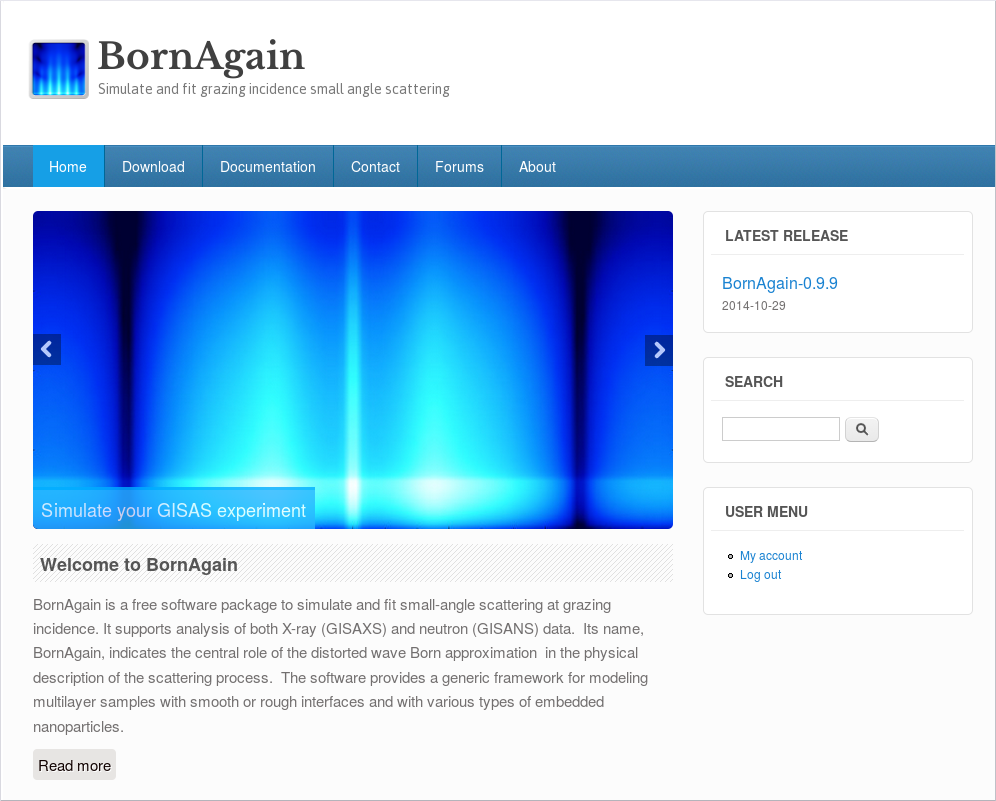
\includegraphics[width=0.83\textwidth]{fig/screenshot/website.png}
\end{center}
\caption{A screenshot of the home page
         \url{http://www.bornagainproject.org}.}
\label{fig:website}
\end{figure}


%%%%%%%%%%%%%%%%%%%%%%%%%%%%%%%%%%%%%%%%%%%%%%%%%%%%%%%%%%%%%%%%%%%%%%%%%%%%%%%%
\section{Download and installation}
%%%%%%%%%%%%%%%%%%%%%%%%%%%%%%%%%%%%%%%%%%%%%%%%%%%%%%%%%%%%%%%%%%%%%%%%%%%%%%%%
  \index{Download}
  \index{Installation}

The \textsc{Download} section on the \BornAgain\ web site
points to the download location for
binary and source packages.
It also provides a link to our \Code{git} server
where the unstable development trunk is available
for contributors or for users who want to live on the edge.

The \textsc{Documentation} section contains
pages with \textit{Installation instructions}.


%%%%%%%%%%%%%%%%%%%%%%%%%%%%%%%%%%%%%%%%%%%%%%%%%%%%%%%%%%%%%%%%%%%%%%%%%%%%%%%%
\section{Further online information}
%%%%%%%%%%%%%%%%%%%%%%%%%%%%%%%%%%%%%%%%%%%%%%%%%%%%%%%%%%%%%%%%%%%%%%%%%%%%%%%%

The \textsc{Documentation} section of the project web site
contains in particular
\begin{itemize}
\item an overview of the software architecture,
\item a list of implemented functionality,
\item tutorials for ``Working with \BornAgain'',
      using either the Graphical User Interface or
      \Python\ scripts,
         \index{Tutorials}
\item a comprehensice collection of examples that demonstrate
   how to use \BornAgain\ for modelling various sample structures
    and different experimental conditions,
\item a link to the API reference for using \BornAgain\ through
   \Python\ scripts or C$++$ programs.
\index{API}%
\index{Application Programming Interface (API)}%
\index{Python}%
\index{C++@C$++$}
\end{itemize}


%%%%%%%%%%%%%%%%%%%%%%%%%%%%%%%%%%%%%%%%%%%%%%%%%%%%%%%%%%%%%%%%%%%%%%%%%%%%%%%%
\section{Registration, contact, discussion forum}
%%%%%%%%%%%%%%%%%%%%%%%%%%%%%%%%%%%%%%%%%%%%%%%%%%%%%%%%%%%%%%%%%%%%%%%%%%%%%%%%

\index{Registration}
\index{Newsletter}
To stay informed about the ongoing development of \BornAgain,
register on the project homepage \url{http://www.bornagainproject.org}
(``Create new account'').
You will then receive our occasional newsletters,
and be authorized to post to the discussion forum

\index{Authors!contact}
\index{Contact}
\index{Discussion forum}
To contact the \BornAgain\ development and maintenance team
in the Scientific Computing Group
of Heinz Maier-Leibnitz Zentrum (MLZ) Garching,
write a mail to \url{contact@bornagainproject.org},
or fill the form in the \textsc{Contact} section of the
project web site.

\index{Forum}
For questions that might be of wider interest,
please consider posting to the discussion forum,
accessible through the \textsc{Forums} tab of the project web site.

%%%%%%%%%%%%%%%%%%%%%%%%%%%%%%%%%%%%%%%%%%%%%%%%%%%%%%%%%%%%%%%%%%%%%%%%%%%%%%%%
%%
%%   BornAgain User Manual
%%
%%   homepage:   http://www.bornagainproject.org
%%
%%   copyright:  Forschungszentrum Jülich GmbH 2015
%%
%%   license:    Creative Commons CC-BY-SA
%%   
%%   authors:    Scientific Computing Group at MLZ Garching
%%               C. Durniak, M. Ganeva, G. Pospelov, W. Van Herck, J. Wuttke
%%
%%%%%%%%%%%%%%%%%%%%%%%%%%%%%%%%%%%%%%%%%%%%%%%%%%%%%%%%%%%%%%%%%%%%%%%%%%%%%%%%


\chapter{Foundations of GISAS}  \SecLabel{ScatTheory}

\newcommand{\nz}{\overline{n}}

%%%%%%%%%%%%%%%%%%%%%%%%%%%%%%%%%%%%%%%%%%%%%%%%%%%%%%%%%%%%%%%%%%%%%%%%%%%%%%%%
\section{Wave propagation}
%%%%%%%%%%%%%%%%%%%%%%%%%%%%%%%%%%%%%%%%%%%%%%%%%%%%%%%%%%%%%%%%%%%%%%%%%%%%%%%%
\index{Wave propagation|(}

%===============================================================================
\subsection{X-ray propagation}
%===============================================================================
\index{Wave propagation!X-rays}
\index{X-rays!wave propagation}

\ldots to come

%===============================================================================
\subsection{Neutron propagation}
%===============================================================================
\index{Wave propagation!neutrons}
\index{Neutrons!wave propagation}

In a GISANS experiment,
we are only interested in small scattering vectors~$\vect{q}$,
and therefore do not register ordinary Bragg scattering
by crystal lattices or other correlations at atomic level;
at most, Bragg scattering must be accounted for as a loss channels.
We therefore describe the neutron-sample interaction
in continuum approximation by a refractive index~$n$ with
\begin{equation}\label{eq:nRefrIndx}
  n^2=1-\frac{4\pi}{K^2}\rho_s
\end{equation}
where $\rho_s$ is an effective scattering length density
\cite{Lax51,Sea89}.
\index{Scattering length density}

%TODO: how is absorption taken into account?

%===============================================================================
\subsection{Helmholtz equation}
%===============================================================================

X-ray and neutron propagation are both governed by
the same stationary wave equation,
the \textit{Helmholtz equation}
\index{Helmholtz equation}
\index{Wave equation}
\begin{equation}\label{eq:Helmholtz}
  \left(\Nabla^2+K^2n(\vect{r})^2\right)\Psi(\vect{r}),
\end{equation}
where $K=2\pi/\lambda_0$ is the vacuum wave number,
and $n$ is the refractive index.
\index{Refractive index}
In this equation,
the time dependence ${\rm e}^{i\omega t}$ of the wave field
does not appear explicitly.
In GISAS, we are only interested in elastic scattering.
Therefore, the wave frequency~$\omega$ is considered constant.

Implicitly, $K$ depends on~$\omega$ through a \textit{dispersion relation}.
\index{dispersion relation}
This relation is fundamentally different for
X-rays (where it is linear, $\omega\propto K$)
and for thermal neutrons (where it is quadratic, $\omega\propto K^2$).
However, for stationary problems
this frequency dependence of~$K$ does not matter.
Therefore we can use $K$ instead of~$\omega$ as a constant
that characterizes the incoming radiation.
In this way, scalar X-ray and neutron scattering can be described by exactly
the same wave equation~(\ref{eq:Helmholtz}).

\index{Wave propagation|)}


%%%%%%%%%%%%%%%%%%%%%%%%%%%%%%%%%%%%%%%%%%%%%%%%%%%%%%%%%%%%%%%%%%%%%%%%%%%%%%%%
\section{Scalar scattering}
%%%%%%%%%%%%%%%%%%%%%%%%%%%%%%%%%%%%%%%%%%%%%%%%%%%%%%%%%%%%%%%%%%%%%%%%%%%%%%%%

For both X-rays and neutrons the refractive index~$n$ is close to~1.
In the following,
we shall use this fact to solve the Helmholtz equation 
in a perturbation expansion
that is known as the Born approximation
though it goes back to Lord Rayleigh
who devised it for the scattering of sound,
and later also applied it to electromagnetic waves.

%===============================================================================
\subsection{Born approximation}
%===============================================================================

We rewrite the scalar Helmholtz equation~(\ref{eq:Helmholtz}) as
\begin{equation}\label{eq:HelmholtzInhomog}
  \left(\Nabla^2+K^2\right)\Psi(\vect{r})
  = \frac{\chi(\vect{r})}{4\pi}\Psi(\vect{r})
\end{equation}
with
\begin{equation}\label{eq:ChiDef}
  \chi(\vect{r}) := \frac{4\pi}{K^2}\left(1-n^2(\vect{r})\right).
\end{equation}
For neutrons, this definition just compensates (\ref{eq:nRefrIndx})
so that $\chi=\rho_s$.
Equation~(\ref{eq:Helmholtz}) looks
like an inhomogenous differential equation ---
provided we neglect for a moment that unknown function~$\Psi$
reappears on the right side.
The homogeneous equation
\begin{equation}\label{eq:HelmholtzHomog}
  \left(\Nabla^2+K^2\right)\Psi_0(\vect{r}) = 0
\end{equation}
is solved by plane waves and superpositions thereof.
For an isolated inhomogeneity,
\begin{equation}\label{eq:HelmholtzForGreen}
  \left(\Nabla^2+K^2\right)G(\vect{r}) = \delta(\vect{r})
\end{equation}
is solved by the Green function\footnote
{Verification under the condition $\vect{r}\ne0$
is a straightforward exercice in vector analysis.
For the special case $\vect{r}=0$,
one encloses the origin in a small sphere
and integrates by means of the Gauß-Ostrogadsky divergence theorem.
This explains the appearance of the factor $4\pi$.}
\begin{equation}\label{eq:Greens1}
  G(\vect{r}) = \frac{{\rm e}^{iKr}}{4\pi r},
\end{equation}
which is an outgoing spherical wave originating from $\vect{r}=0$.
Convoluting this function with the given inhomogeneity $(\chi/4\pi)\Psi$,
we obtain the formal solution
of the full inhomogeneous equation~(\ref{eq:HelmholtzInhomog})
\begin{equation}\label{eq:PsiFormal}
  \Psi(\vect{r})
  = \Psi_0(\vect{r})
  + \int\,{\rm d}^3r' G(\vect{r}-\vect{r'})
                     \frac{\chi(\vect{r'})}{4\pi}\Psi(\vect{r'}).
\end{equation}
However, the integral kernel still contains the full solution~$\Psi$.
If we replace this occurence of $\Psi$
by the full right-hand side of~(\ref{eq:PsiFormal})
we obtain
\begin{equation}
  \Psi(\vect{r})
  = \Psi_0(\vect{r})
  + \int\,{\rm d}^3r' G(\vect{r}-\vect{r'})\frac{\chi(\vect{r'})}{4\pi}
  \left(\Psi_0(\vect{r'})
  + \int\,{\rm d}^3r''
  G(\vect{r'}-\vect{r''})\frac{\chi(\vect{r''})}{4\pi}
  \Psi(\vect{r''})\right).
\end{equation}
This can be iterated to obtain an infinite series representation of $\Psi$.
Successive terms in this series contain rising powers of $\chi$.
Since $\chi$ is assumed to be small, the series is likely to converge.
In first Born approximation,
only the linear order in $\chi$ is retained,
\begin{equation}\label{eq:Born}
  \Psi(\vect{r})
  \simeq \Psi_0(\vect{r})
  + \int\,{\rm d}^3r' G(\vect{r}-\vect{r'})\frac{\chi(\vect{r'})}{4\pi}
   \Psi_0(\vect{r'}).
\end{equation}
This is practically always adequate for
material investigations with X-rays or neutrons,
where the aim is to 
deduce $\chi(\vect{r'})$ from the scattered intensity ${|\Psi(\vect{r})|}^2$.

%===============================================================================
\subsection{Far-field expansion}
%===============================================================================

In a scattering experiment,
the intensity ${|\Psi(\vect{r})|}^2$ is measured
at a detector location~$\vect{r}$
far away from the sample volume.
We choose the coordinate origin at the nominal center of the sample
so that the integral in~(\ref{eq:Born}) runs over $\vect{r'}$ with $r'\ll r$.
This allows us to expand
\begin{equation}
  \left|\vect{r}-\vect{r'}\right|
  \simeq \sqrt{r^2-2\vect{r}\,\vect{r'}}
  \simeq r - \frac{\vect{r}\,\vect{r'}}{r}
  \equiv r - \frac{\vect{k}_f \vect{r'}}{K},
\end{equation}
where we have introduced the outgoing wave vector
\begin{equation}
  \vect{k}_f:=K\frac{\vect{r}}{r}.
\end{equation}
We apply this to the Green function~(\ref{eq:Greens1}),
retaining the first order in $\vect{r'}$ in the exponent,
but not in the denominator:
\begin{equation}
  G(\vect{r}-\vect{r'})
  \simeq\frac{{\rm e}^{iKr - i\vect{k}_f \vect{r'}}}{4\pi r}.
\end{equation}
This is an outgoing spherical wave with respect to $\vect{r}$,
but a plane wave with respect to~$\vect{r'}$.
If the incident radiation is also a plane wave,
\begin{equation}\label{eq:Psi0Plane}
  \Psi_0(\vect{r})={\rm e}^{i \vect{k}_i \vect{r}},
\end{equation}
then the Born approximation~(\ref{eq:Born})
becomes essentially a Fourier transform of $\chi$,
  \index{Fourier transform}
\begin{equation}\label{eq:BornPlane}
  \Psi(\vect{r})
  \simeq \Psi_0(\vect{r})
  + \frac{{\rm e}^{iKr}}{r}
    \int\,{\rm d}^3r' {\rm e}^{i\vect{q}\,\vect{r'}}\chi(\vect{r'})
\end{equation}
with the \textit{scattering vector}
\index{Scattering vector}
\begin{equation}
  \vect{q}:=\vect{k}_i-\vect{k}_f.
\end{equation}

%===============================================================================
\subsection{Differential cross section}
%===============================================================================

Above, we said somewhat sloppily
that a scattering experiment measures intensities~${|\Psi(\vect{r}|}^2$.
We shall now make this more rigorous.
In the case of neutron scattering,
one actually measures the probability flux.
We define it in arbitrary relative units as
\begin{equation}
  \vect{J} := \Psi^*\frac{\Nabla}{2i}\Psi - \Psi\frac{\Nabla}{2i}\Psi^*.
\end{equation}
With (\ref{eq:Psi0Plane}), the incident flux is
\begin{equation}
  \vect{J}_0 = \vect{k}_i.
\end{equation}
The scattered wavefield (\ref{eq:BornPlane}) is observed
at a detector position $\vect{r}$ that is not illuminated by the
incident beam, hence $\Psi_0(\vect{r})=0$.
This leaves us with
\begin{equation}
  \vect{J}(\vect{r})
  = {\left|\frac{1}{r}
    \int\,{\rm d}^3r' {\rm e}^{i\vect{q}\,\vect{r'}}\chi(\vect{r'})
    \right|}^2 K\frac{\vect{r}}{r}.
\end{equation}
The ratio of the scattered current hitting an infinitesimal detector area
$r^2{\rm d}\Omega$ to the incident flux is expressed as a
\textit{differential cross section}
  \index{Cross section}
  \index{Differential cross section}
\begin{equation}
  \frac{{\rm d}\sigma}{{\rm d}\Omega}
  := \frac{r^2 J(\vect{r})}{J_0}.
\end{equation}
Using $k_i=K$ and changing notation $\vect{r'}\to\vect{r}$,
we find
\begin{equation}
  \frac{{\rm d}\sigma}{{\rm d}\Omega}
  = {\left|
    \int\,{\rm d}^3r {\rm e}^{i\vect{q}\,\vect{r}}\chi(\vect{r})
    \right|}^2 =: {\left| \chi(\vect{q}) \right|}^2
\end{equation}
The differential cross section is just the squared modulus
of the Fourier transform $\chi(\vect{q})$
\index{Fourier transform}
of the scattering-length distribution~(\ref{eq:ChiDef}).


%%%%%%%%%%%%%%%%%%%%%%%%%%%%%%%%%%%%%%%%%%%%%%%%%%%%%%%%%%%%%%%%%%%%%%%%%%%%%%%%
\section{Distorted Wave Born Approximation} 
%%%%%%%%%%%%%%%%%%%%%%%%%%%%%%%%%%%%%%%%%%%%%%%%%%%%%%%%%%%%%%%%%%%%%%%%%%%%%%%%
\index{Distorted wave Born approximation}
\index{DWBA|see {Distorted wave Born approximation}}

As we have seen
the Born approximation relies on plane waves,
which basically means that incoming and scattered radiation
are assumed to propagate along straight lines,
with directions expressed by $\vect{k}_i$ and $\vect{k}_f$.
This is adequate for most experiments with weakly interacting radiation,
and especially for most X-ray and neutron scattering techniques,
but not for grazing-incidence small-angle scattering
where radiation is refracted and reflected by interfaces
 \index{Refraction}
 \index{Reflection}
and therefore does not propagate along straight lines.
The Born approximation also fails for collisions of charged particles.
For them, Massey and Mott devised in the early 1930s
the distorted wave Born approximation (DWBA).
% Schiff (^3 1968, p 327) cites
% Mott, Massey, The Theory of Atomic Collisions, p 100, Oxford 1933;
% There are also several papers by Massey and Mott from about 1933.
A particularly simple variant of this approximation
is routinely used to account for refraction and reflection
in grazing-incidence scattering.

In reflectometry or grazing-incidence scattering,
samples are usually modelled as being translationally invariant
in $x$ and $y$ direction,
while being nontrivially modulated in $z$ direction.
The $z$ axis points upwards, hence out of the sample towards the
air or vacuum half space where the incident radiation comes from.
% TODO: add figure

Refraction and reflection are caused by vertical variations
of the average refractive index $\nz(z)$.
We rewrite the Helmholtz equation~(\ref{eq:HelmholtzInhomog} as
\begin{equation}\label{eq:HelmholtzGraded}
  \left(\Nabla^2+K^2\nz^2(z)\right)\Psi(\vect{r})
  = \frac{\chi(\vect{r})}{4\pi}\Psi(\vect{r})
\end{equation}
with (\ref{eq:ChiDef}) replaced by
\begin{equation}\label{eq:ChiGraded}
  \chi(\vect{r}) := \frac{4\pi}{K^2}\left(\nz^2(z)-n^2(\vect{r})\right).
\end{equation}
The homogeneous equation
\begin{equation}\label{eq:HelmholtzGradedHomog}
  \left(\Nabla^2+K^2\nz^2(z)\right)\Psi_0(\vect{r}) = 0
\end{equation}
suggests the ansatz
\begin{equation}\label{eq:wave3}
\psi_0(\vect{r}) = {\rm e}^{i \vect{k}_\parallel\vect{r}_\parallel} \phi(z).
\end{equation}
The in-plane wave vector $\vect{k}_\parallel$ remains constant
as initialized by the incoming beam.
The vertical wave function must fulfill
\begin{equation}\label{eq:wavez}
\left(\partial_z^2 + K^2\nz(z)^2 - k_\parallel^2 \right) \phi(z) = 0.
\end{equation}
Since we are describing scattering in continuum approximation anyway,
we can safely assume that $\nz(z)$ varies only slowly on the length scale
of the radiation wavelength.
Therefore an appropriate ansatz is
\begin{equation}
  \phi(z) = r(z){\rm e}^{ip(z)z} + t(z){\rm e}^{-ip(z)z}
\end{equation}
with
\begin{equation}
  p(z) := \sqrt{K^2\nz(z)^2 - k_\parallel^2}.
\end{equation}
Since the incoming beam has a vertical component in direction $-z$,
we identify $r(z)$ and $t(z)$
as amplitudes of the backward-propagating (reflected)
and forward-propagting (transmitted) beam, respectively.

%===============================================================================
\subsection{Multilayer systems}
%===============================================================================

In multilayer systems, the first term of (\ref{eq:tdwba}) denotes the specular part of the reflection, while the second term is responsible for the off-specular scattering. This off-specular part is caused by deviations from the perfectly smooth layered system, as e.g. interface roughnesses or included nanoparticles. In here only the case of nanoparticles will be treated.

In the conventions where $H=-\Delta + V$, the potential splits into two parts $V_1$ and $V_2$, where only the second part is treated as a perturbation:
\begin{align*}
  V_1 & = K^2\left( 1-n_0^2(\vect{r})\right)  \\
  V_2 & = \sum_i K^2\left( n_0^2(\vect{R}^i) - n_i^2 \right) S^i(\vect{r}) \otimes \delta(\vect{r}-\vect{R}^i),
\end{align*}
where $n_0(\vect{r})$ denotes the refractive index of the unperturbed system (which, in case of a multilayer system, will only depend on its $z$-coordinate) and $n_i$ is the refractive index of the nanoparticle with shape function $S^i$ and position $\vect{R}^i$.

For nanoparticles in a specific layer $j$, i.e. $V_2\neq0$ only in layer $j$, one only needs the unperturbed solutions in layer $j$:
\begin{align*}
  \braketnoop{\vect{r}}{\Psi^+_{1k_i}} &= (2\pi)^{-3/2}\left[ R_j(\vect{k}_i) e^{i \vect{k}_{j,R}(\vect{k}_i)\cdot\vect{r}} + T_j(\vect{k}_i) e^{i \vect{k}_{j,T}(\vect{k}_i)\cdot\vect{r}} \right] \\
  \braketnoop{\Psi^-_{1k_f}}{\vect{r}} &= (2\pi)^{-3/2}\left[ R_j(-\vect{k}_f) e^{i \vect{k}_{j,R}(-\vect{k}_f)\cdot\vect{r}} + T_j(-\vect{k}_f) e^{i \vect{k}_{j,T}(-\vect{k}_f)\cdot\vectr} \right].
\end{align*}

The off-specular contribution to the scattering amplitude then becomes:
\begin{align*}
  f(\theta, \phi) &= -\int d^3\vectr \frac{V_2(\vectr)}{4\pi} \biggl[ T_iT_fe^{i(\vectk_{j,i}-\vectk_{j,f})\cdot\vectr} + R_iT_fe^{i(\vectkt_{j,i}-\vectk_{j,f})\cdot\vectr} \\
   & + T_iR_fe^{i(\vectk_{j,i}-\vectkt_{j,f})\cdot\vectr} + R_iR_fe^{i(\vectkt_{j,i}-\vectkt_{j,f})\cdot\vectr} \biggr],
\end{align*}
where the following shorthand notations were used:
\begin{align*}
  T_i &\equiv  T_j(\vect{k}_i) & R_i &\equiv  R_j(\vect{k}_i)  \\
  T_f &\equiv  T_j(-\vect{k}_f) & R_f &\equiv  R_j(-\vect{k}_f) \\
  \vectk_{j,i} &\equiv \vectk_{j,T}(\vectk_i) & \vectkt_{j,i} &\equiv \vectk_{j,R}(\vectk_i)  \\
  \vectk_{j,f} &\equiv -\vectk_{j,T}(-\vectk_f) & \vectkt_{j,f} &\equiv -\vectk_{j,R}(-\vectk_f).
\end{align*}

From this expression, one sees that the scattering amplitude consists of a weighted sum of Fourier transforms of the potential $V_2$. Using
\begin{equation*}
  V_2(\vectr) = \sum_i 4\pi \rho_{s,rel,i} S^i(\vectr) \otimes \delta(\vectr - \vect{R}^i),
\end{equation*}
with $\rho_{s,rel,i}\equiv  K^2\left( n_0^2(\vect{R}^i) - n_i^2 \right)/4\pi$, the scattering amplitude becomes
\begin{equation*}
  f(\theta, \phi) = -\sum_i  \rho_{s,rel,i} \curlf^i_{\text{DWBA}}(\vectk_{j,i},\vectk_{j,f},\vect{R}^i_z)e^{i(\vectk_{j,i\parallel}-\vectk_{j,f\parallel})\cdot \vect{R}^{i\parallel} },
\end{equation*}
with
\begin{align*}
  \curlf^i_\text{DWBA}(\vectk_i,\vectk_f,R_z) & \equiv T_iT_fF^i(\vectk_i-\vectk_f)e^{i(k_{iz}-k_{fz})R_z} + R_iT_fF^i(\vectkt_i-\vectk_f)e^{i(-k_{iz}-k_{fz})R_z} \\
  & + T_iR_fF^i(\vectk_i-\vectkt_f)e^{i(k_{iz}+k_{fz})R_z} + R_iR_fF^i(\vectkt_i-\vectkt_f)e^{i(-k_{iz}+k_{fz})R_z},
\end{align*}

TO MERGE IN:
In the DWBA, the form factor of a particle in a multilayer system is given by
\begin{align}
F_{\rm{DWBA}} (\vect{k}_i,\vect{k}_f, r_z) & = T_i T_f F_{\rm{BA}} (\vect{k}_i-\vect{k}_f) e^{i (k_{i,z}-k_{f,z}) r_z} + R_i T_f F_{\rm{BA}}(\vect{\widetilde{k}}_i-\vect{k}_f) e^{i(-k_{i,z}-k_{f,z})r_z}
 \nonumber \\
  &+ T_i R_f F_{\rm{BA}}(\vect{k}_i-\vect{\widetilde{k}}_f)e^{i(k_{i,z}+k_{f,z})r_z} + R_iR_fF_{\rm{BA}} (\vect{\widetilde{k}}_i-\vect{\widetilde{k}}_f)e^{i(-k_{i,z}+k_{f,z})r_z}, \label{eq:dwbageneral}
\end{align}
where $F_{\rm{BA}}$ is the expression of the form factor in the Born approximation, $r_z$ is the $z$-coordinate of the particle's position (measured from the bottom of the particle), $\vect{k}_i=(k_{i,x}, k_{i,y}, k_{i,z})$ $\vect{k}_f=(k_{f,x}, k_{f,y}, k_{f,z})$ are the incident and scattered wave vectors in air, respectively \cite{RaSS95}.
With a tilde (\~{}), these wave vectors components are evaluated in the multilayer system (the refractive indices of the different constituting materials have to be taken into account). 
$T_i$, $T_f$, $R_i$, $R_f$ are the transmission and reflection coefficients for the incident wave (index $i$) or the scattered one (index $f$). These coefficients can be calculated using the Parratt formalism \cite{Par54} or the matrix method \cite{BoWo99}. $\vect{k}_i-\vect{k}_f$ is equal to the scattering vector $\vect{q}$ and the $z$-axis is pointing upwards.\\

With this last expression, the same techniques as demonstrated in section \ref{sec:ba} can be applied, leading to the following expression for the expectation value of the scattering cross-section:
\begin{align*}
  & \left\langle \frac{d\sigma}{d\Omega}(\vectk_i,\vectk_f) \right\rangle_{\text{Off-specular}}  \\
  & = \sum_\alpha p_\alpha \left\lvert \curlf_\alpha(\vectk_{j,i},\vectk_{j,f}, R_{\alpha,z})\right\rvert ^2 + \frac{\rho_S}{S}\sum_{\alpha,\beta} p_\alpha p_\beta \curlf_\alpha (\vectk_{j,i},\vectk_{j,f}, R_{\alpha,z})\curlf_\beta^*(\vectk_{j,i},\vectk_{j,f}, R_{\beta,z}) \\
  & \times \iint_S d^2\vect{R}_\alpha^\parallel d^2\vect{R}_\beta^\parallel \ppcf{\alpha}{\beta}{R^\parallel} \exp \left[ i\vect{q}_{j\parallel}\cdot (\vect{R}_\alpha^\parallel - \vect{R}_\beta^\parallel ) \right].
\end{align*}

The main differences with respect to the cross-section in the Born approximation are:
\begin{enumerate}
  \item The particle form factor now consists of a more complex expression and now depends on both incoming and outgoing wavevectors and also on the $z$-coordinate of the particle;
  \item Since the $z$-coordinate of the particles is implicitly included in its formfactor, the position integrals only run over $x$- and $y$-coordinates and the volume and density gets replaced with the surface area and surface density respectively.
\end{enumerate}

%===============================================================================
\section{Polarization}
%===============================================================================

ome GISAS experiments are performed with polarized radiation
or/and involve polarization-dependent interactions.
Therefore we need also to consider
the propagation of polarized X-rays and neutrons.
Electromagnetic field vectors and neutron spinors
are fundamentally different mathematical objects
Nevertheless, for our purpose they can be
mapped onto a uniform .... <to elaborate> ....
so that one and the same formalism can be applied
to polarized GISAXS and GISANS.
This shall be derived in the following.


%===============================================================================
\subsection{Polarized X-rays}
%===============================================================================

%===============================================================================
\subsection{Polarized neutrons}
%===============================================================================




%===============================================================================
\section{TO RECYCLE}
%===============================================================================

Consider a scattering volume $V$, containing $N$ scattering centers with shape functions $S^i(\vect{r})$, positions $\vect{R}^i$ and scattering length density $\rho_s$ (relative to the ambient material).

The differential cross-section (per scattering center) is then given by:
\begin{equation}\label{eq:xsec1}
  \frac{d\sigma}{d\Omega}(\vect{q}) = \frac{1}{N}\left\lvert \int_V \rho_s(\vect{r}) e^{i\vect{q}\cdot\vect{r}} d^3\vect{r} \right\rvert ^2.
\end{equation}


%%%%%%%%%%%%%%%%%%%%%%%%%%%%%%%%%%%%%%%%%%%%%%%%%%%%%%%%%%%%%%%%%%%%%%%%%%%%%%%%
%%
%%   BornAgain User Manual
%%
%%   homepage:   http://www.bornagainproject.org
%%
%%   copyright:  Forschungszentrum Jülich GmbH 2015
%%
%%   license:    Creative Commons CC-BY-SA
%%   
%%   authors:    Scientific Computing Group at MLZ Garching
%%               C. Durniak, M. Ganeva, G. Pospelov, W. Van Herck, J. Wuttke
%%
%%%%%%%%%%%%%%%%%%%%%%%%%%%%%%%%%%%%%%%%%%%%%%%%%%%%%%%%%%%%%%%%%%%%%%%%%%%%%%%%


\chapter{DWBA for multilayer systems}  \label{sec:Multilayers}


\index{Multilayer|(}%
\index{Layer structures|see {Multilayer}}

In Sect.~\ref{Sdwba},
we have discussed wave propagation and scattering in 2$+$1 dimensional systems
that are translationally invariant in the horizontal $xy$ plane,
and have a vertical refractive index profile $\nz(z)$.
Here we specialize to layered systems
where $\nz(z)$ is a step function that is constant within one layer.
First, only scalar interactions are considered.
Later, the theory is extended to account for polarization effects.

\Note{\indent By convention,
layers are numbered from top to bottom.
The top vacuum (or air) layer (which extends to $z\to+\infty$) has number~0,
the substrate (extending to $z\to-\infty$) is layer~$N$.}

All layer interfaces are assumed to be perfectly smooth.
For rough interfaces, see Chapter~\ref{sec:Roughness}.

%%%%%%%%%%%%%%%%%%%%%%%%%%%%%%%%%%%%%%%%%%%%%%%%%%%%%%%%%%%%%%%%%%%%%%%%%%%%%%%%
\section{Scalar case}
%%%%%%%%%%%%%%%%%%%%%%%%%%%%%%%%%%%%%%%%%%%%%%%%%%%%%%%%%%%%%%%%%%%%%%%%%%%%%%%%

%===============================================================================
\subsection{Wave propagation and DWBA matrix element}
%===============================================================================

\index{Multilayer!Indexing convention}%

To compute scattering cross sections in DWBA,
we first need to determine the distorted wave functions~$\psi_w(\r)$
for $\r$ inside the sample.
The following derivation holds for the incoming wave ($w=\ti$)
as well as for the back-traced detected wave ($w=\tf$).

We consider wave propagation in one layer~$j$
\nomenclature[2j020]{$j$}{Index of layer in multilayer sample}%
with constant average refractive index $\nz(z)=\nzj$.
A vacuum plane wave, impinging on a layered structure,
is at each interface partly reflected, partly refracted,
so that the wave function inside a material layer
has an upward and a downward propagating component,
as per~(\ref{Epsipm}).
Each component is a plane wave,
\begin{equation}
  \psi^\pm_{wj}(\r)=\e^{i\k^\pm_{\parallel w}\r_\parallel}\phi^\pm_{wj}(z)
\end{equation}
with
\begin{equation}\label{Ephizwj}
  \phi^\pm_{wj}(\r)=A^\pm_{wj}\e^{\pm i\k_{\perp wj}(z-z_j)}.
\end{equation}
\nomenclature[2a123 2w010 2j010 \pm]{$A^\pm_{wj}$}{Amplitude of the plane wave $\phi^\pm_{wj}(\r)$}%
For later convenience,
the phase factor in (\ref{Ephizwj}) includes an offset
given by~$z_j$, the $z$ coordinate at the bottom of layer~$j$.
The amplitudes $A$ are often written with distinct letters
T and~R to designate the transmitted or reflected beam,
\begin{equation}
  T_{wj} := A^-_{wj},\quad
  R_{wj} := A^+_{wj}.
\end{equation}
\nomenclature[2t126 2w020 2j020 0]{$T_{wj}$}{Partial amplitude of $\psi_w(\r)$
  in layer $j$ in downward (transmission) direction, also denoted $A^-_{wj}$}%
\nomenclature[2r126 2w020 2j020 0]{$R_{wj}$}{Partial amplitude of $\psi_w(\r)$
  in layer $j$ in upward (reflection) direction, also denoted $A^+_{wj}$}%
They need to be computed recursively,
as described in the following subsection~\ref{Sacrolay}.

Each plane wave component $\psi^\pm_{wj}(\r)$ has
a three-dimensional wave vector
\begin{equation}\label{Ekpmwj3}
  \k^\pm_{wj}= \k_{\parallel w} \pm k_{\perp wj}\v{\hat z}.
\end{equation}
\nomenclature[2z060]{$\v{\hat z}$}{Unit vector along the sample normal}%
\nomenclature[2k043 2w010 2j010 \pm]{$\k^\pm_{wj}$}{Wave vector of the plane wave $\Psi^\pm_{wj}(\r)$}%
As explained in connection with~(\ref{Ekpar}),
the in-plane wave vector $\k_{\parallel w}$ remains constant
across layer interfaces.
The vertical wavenumber is obtained from (\ref{Ewavez}),
\begin{equation}\label{Ekperpwj}
  k_{\perp wj} = \sqrt{K^2 \nzj - k_{\parallel w}^2}.
\end{equation}
The glancing angle is
\begin{equation}\label{Edef_alpha}
  \alpha_{wj}:=\arctan(k_{\perp wj}/k_{\parallel w}).  
\end{equation}
Equivalently,
\begin{equation}
  k_{\parallel w}=K n_j \cos\alpha_{wj}. 
\end{equation}
Since $k_{\parallel w}$ is constant across layers,
we have
\begin{equation}\label{ESnell}
  n_j \cos\alpha_{wj} = \text{the same for all }j,
\end{equation}
which is Snell's refraction law.
\index{Refraction!Snell's law}
\index{Snell's law}

Since the $\psi^\pm_{wj}$ are plane waves within layer~$j$,
we can at once write down the DWBA transition matrix~(\ref{EtmDWBAsum})
\index{Distorted-wave Born approximation!multilayer}%
\Emph{
\begin{equation}\label{EtmDWBAft}
  \bra \Psi_\tf|\chi|\Psi_\ti\ket
  = \sum_{j} \sum_{\pm_\tf} \sum_{\pm_\ti}
    A^\pm_{\ti j} A^{\pm *}_{\tf j}
     \chi_j(\k^\pm_{\ti j} - \k^\pm_{\tf j})
\end{equation}\vspace*{-5pt}
}
where
\begin{equation}\label{Echij}
  \chi_j(\v{q})
  := \int_{z_j}^{z_{j-1}}\!\d z \int\!\d^2r_\parallel\, \e^{i\v{q}\,\r}\chi(\r)
\end{equation}
\nomenclature[1χ032 2j010 2q040]{$\chi_j(\v{q})$}{Fourier transform of the perturbation potential $\chi(\r)$, evaluated in one sample layer}%
is the Fourier transform
of the perturbative potential~(\ref{EChiGraded}),
restricted to one layer.

%-------------------------------------------------------------------------------
\subsection{Wave propagation across layers}\label{Sacrolay}
%-------------------------------------------------------------------------------

\index{Fresnel coefficients}%
\index{Transmission|see {Fresnel coefficients}}%
\index{Reflection|seealso {Fresnel coefficients}}%

The plane-wave amplitudes $A^\pm_{wj}$ need to be computed recursively
from layer to layer.
Since these computations are identical for incident and final waves,
we omit the subscript~$w$ in the remainder of this section.
At layer interfaces, the optical potential changes discontinuously.
From elementary quantum mechanics we know that
piecewise solutions of the Schrödinger equations must be connected
such that the wave function $\phi(\r)$ and its first derivative
$\Nabla\phi(\r)$ evolve continuously.
This means for the interface
at the \textit{bottom} of layer~$j=0,\ldots,N-1$:%
\begin{equation}\label{Econtcond}
  \begin{array}{lcl}
            \phi_j(z_j)&=&\phi_{j+1}(z_{j+1}+d_{j+1}),\\
            \partial_z\phi_j(z_j)&=&\partial_z\phi_{j+1}(z_{j+1}+d_{j+1}),
  \end{array}
\end{equation}
  where
\begin{equation}
  d_j:=z_{j-1}-z_{j}
\end{equation}
is the thickness of layer~$j$.

We abbreviate
\begin{equation}
  f_j := k_{\perp j}/K = \sqrt{\overline{n_j^2}-(k_\parallel/K)^2}
\end{equation}
and
\begin{equation}
   \delta_j := \e^{iKf_jd_j}.
\end{equation}
For the plane waves (\ref{Ephizwj}),
the continuity conditions~(\ref{Econtcond}) take the form
\begin{equation}\label{Econt2}
  \begin{array}{lclclcl}
  A^+_j &+& A^-_j,
  &=&
  a_{j+1}\delta_{j+1} &+& A^-_{j+1}\delta_{j+1}^*,
  \\
  A^+_j f_j  &-& A^-_j f_j,
  &=&
 a_{j+1}\delta_{j+1} f_{j+1} &-& A^-_{j+1}\delta_{j+1}^* f_{j+1}.
  \end{array}
\end{equation}
After some lines of linear algebra,
we can rewrite this equation system as
\begin{equation}\label{EcMc}
  \left( \begin{array}{c}A^+_j\\A^-_j\end{array} \right)
  = M_{j+1} \left( \begin{array}{c}A^+_{j+1}\\A^-_{j+1}\end{array} \right)
\end{equation}
with the transfer matrix
\begin{equation}
  M_j
   = \frac{1}{2f_{j-1}}
   \left(\begin{array}{cc}
       \delta_j(f_{j-1}+f_j)&\delta_j^*(f_{j-1}-f_j)\\
       \delta_j(f_{j-1}-f_j)&\delta_j^*(f_{j-1}+f_j)
   \end{array}\right).
\end{equation}
To study wave propagation across the entire stack of layers,
we use the combined transfer matrix
\begin{equation}
   M = M_1 \cdots M_N.
\end{equation}
In our scattering setup,
plane-wave amplitudes are subject to two boundary conditions:
In the top layer, $A^-_{w0}=1$ is given by the
incident or back-traced final plane wave.
In the substrate, $A^+_{wN}=0$ because there is no radiation
coming from $z\to-\infty$.
This leaves us with two unkown amplitudes connected by
\begin{equation}
  \left( \begin{array}{c}A^+_0\\1\end{array} \right)
  = M \left( \begin{array}{c}0\\A^-_N\end{array} \right),
\end{equation}
which is solved by
\begin{equation}
  \begin{array}{lcl}
    A^-_N &=& 1/M_{22},\\[.2ex]
    A^+_0 &=& M_{12}/M_{22}.
  \end{array}
\end{equation}
It is a straightforward exercice to verify
that for a single interface between two semi-infinite media,
the reflection and transmission probabilities
agree with Fresnel's result for $s$-polarized light,\footnote
{See any optics textbook, e.~g. Born~\&~Wolf \cite[ch.~1.5.2]{BoWo99}
  or Hecht \cite[ch.~4.6.2]{Hec02}.}
\begin{equation}
  \left| A^+_0\right|^2
  = \left|\frac{f_0-f_1}{f_0+f_1}\right|^2,
  \quad
  \left| A^-_N\right|^2
  = \left| \frac{2f_0}{f_0+f_1}\right|^2.
\end{equation}

\Work{How does the above relate to what is actually computed in BornAgain?
And how to Abeles matrices, Parrat's formalism, Deak's papers?}

%-------------------------------------------------------------------------------
\subsection{Damped waves in absorbing media
  or under total reflection}\label{s:complex}
%-------------------------------------------------------------------------------

In Sect.~\ref{Sabsorption},
we have chosen the horizontal wave vector $\k_{\parallel}$
to be always real and constant.
In contrast, the vertical wave number $k_{\perp j}$,
given by (\ref{Ekperpwj}),
can become imaginary or complex.
If $\overline{n_j^2}$ is real and smaller than~$n_0^2\cos^2\alpha_0$,
then Snell's law of refraction (\ref{ESnell}) cannot be fulfilled,
and the radicand in (\ref{Ekperpwj}) becomes negative
so that $k_{\perp j}$ becomes pure imaginary.
\index{Wave vector!complex}%
If the layer is absorbing,
described by an positive imaginary part of $\overline{n_j^2}$,
then the radicand in (\ref{Ekperpwj}) becomes complex,
and the wave number $k_{\perp j}$ as well.
For complex $k_{\perp j}$,
the theory developed above remains applicable,
except that the geometric interpretation of the wave vectors $\k_\pm$
in Eqs.~(\ref{Edef_alpha}--\ref{ESnell}) is untenable.

Writing
\begin{equation}
  k_\perp = k_\perp' + i k_\perp''
\end{equation}
for a decomposition into a real and an imaginary part,
we find an exponential decay of the plane wave amplitudes
\begin{equation}\label{Ephidamp}
  \left|\phi^\pm_j(z)\right|
  = \e{\mp k_{\perp j}'' z}
\end{equation}
along their propagation direction~$\pm z$.
With an analogous decomposition
of the three-dimensional wave vector (\ref{Ekpmwj3}),
we obtain for the flux, defined as in~(\ref{EdefJ}),
\begin{equation}
  \v{J}_j(\r) = \k' \e^{-2k_{\perp j}z}.
\end{equation}
In the special case of a pure imaginary~$k_{\perp j}$,
the flux direction is $\k'=\k_\parallel$:
$\psi_j(\r)$ is an \textit{evanescent wave},
\index{Evanescent wave}%
travelling horizontally,
and therefore transmitting no radiation intensity to lower layers.
In the stationary state,
all incoming radiation undergoes \textit{total reflection}.
\index{Total reflection}%

In the generic case of a complex~$k_{\perp j}$,
the flux has a vertical component.
Accordingly, the total reflection is not perfect.
Some intensity is dissipated in layer $j$.
\index{Dissipation}%
And if layer $j>N$ is not too thick,
then some radiation intensity also tunnels into the adjecent layer $j+1$.
\index{Tunneling}%


%%%%%%%%%%%%%%%%%%%%%%%%%%%%%%%%%%%%%%%%%%%%%%%%%%%%%%%%%%%%%%%%%%%%%%%%%%%%%%%%
% \newpage % TEMPORARY
\section{Reflection with polarization-dependent interactions}\label{s:pol}
%%%%%%%%%%%%%%%%%%%%%%%%%%%%%%%%%%%%%%%%%%%%%%%%%%%%%%%%%%%%%%%%%%%%%%%%%%%%%%%%

\Work{\indent The following draft must be reworked once
  the chapter on polarized waves propagation is written.}

%\cite{Deak_ppt, PhysRevB.76.224420, Deak2001113, PhysRevB.53.6158}.
%\cite{RevModPhys.23.287}

%-------------------------------------------------------------------------------
\subsection{Wave equation and propagation within one layer}
%-------------------------------------------------------------------------------

To allow for polarization-dependent interactions,
we replace the squared index of refraction $n^2$
by $1+\uu\chi$, where $\uu\chi$ is a $2\times 2$ susceptibility matrix.
The wave equation (\ref{Escalar_wave}) for layer~$j$ becomes
\begin{equation}\label{Ewaveqp}  
(\Delta +K^2 +K^2 \uu\chi_j) \u\psi(\r)= 0,
\end{equation}
where $\u\psi(\r)$ is a two-component spinor wave function,
with components $\psi_\UP(\r)$ and~$\psi_\DN(\r)$.
At interfaces between layers,
both spinor components of $\u\psi(\r)$ and $\Nabla\u\psi(\r)$
must evolve continuously.

The reasons for the factorization (\ref{Ewave3}) still apply,
and so we can write
\begin{equation}\label{Ewave3p}
\u\psi(\r) = \u\psi(z) \e^{i \k_\parallel\r_\parallel}.
\end{equation}
As before, $\k_\parallel$ is constant across layers.
The wave equation~(\ref{Ewaveqp}) reduces to 
\begin{equation}\label{Ewavezp}
\left(\partial_z^2 + K^2 + K^2\uu\chi_j - k_\parallel^2 \right) \u\psi(z) = 0.
\end{equation}
We abbreviate
\begin{equation}
  \uu H_j := K^2(1+\uu\chi_j)-k_\parallel^2
\end{equation}
so that the wave equation becomes simply
\begin{equation}\label{Ewaveqp2}
  \left(\partial_z^2 + \uu H_j\right) \u\psi(z) = 0.
\end{equation}
The solution is
\begin{equation}\label{Epsizp}
  \u\psi_j(z)
  = \sum_{k=1}^2 \u x_{jk}\left(\alpha_{jk}\e^{i p_{jk}(z-z_k)}
                            + \beta_{jk}\e^{-i p_{jk}(z-z_k)}\right),
\end{equation}
where the $\u x_{jk}$ are eigenvectors of $\uu H_j$
with eigenvalues $p_{jk}^2$:
\begin{equation}
  \left( -p_{jk}^2 + \uu H_j \right) \u x_{jk} = 0
   \;\text{ for }\;j=1,2.
\end{equation}
In a reproducible algorithm,
the eigenvectors $\u x_{jk}$ must be chosen according to some arbitrary
normalization rule,
for instance
\begin{equation}
  |\u x_{jk}|=1,\quad x_{ij\UP} \text{ real and nonnegative}.
\end{equation}
Similarly,
a rule is needed how to handle the case of one degenerate eigenvalue,
which includes in particular the case of scalar interactions.


%-------------------------------------------------------------------------------
\subsection{Wave propagation across layers}
%-------------------------------------------------------------------------------

Generalizing (\ref{Evecc}),
we introduce the coefficient vector
\begin{equation}
  c_j := {(\alpha_{j1}, \alpha_{j2}, \beta_{j1}, \beta_{j2})}^\text{T}.
\end{equation}
To match solutions for neighboring layers,
continuity is requested for both spinorial components
of $\u\psi$ and $\Nabla\u\psi$.
As before (\ref{EFcFDc}), we have at the bottom of layer~$j$
\begin{equation}\label{EFcFDcp}
  F_j c_j = F_{j+1} D_{j+1} c_{j+1},
\end{equation}
where the matrices are now
\begin{equation}
  F_j := \left(\begin{array}{cccc}
    x_{i1\UP}      &x_{i2\UP}     &x_{i1\UP}       &x_{i2\UP}       \\
    x_{i1\DN}      &x_{i2\DN}     &x_{i1\DN}       &x_{i2\DN}       \\
    x_{i1\UP}p_{j1}&x_{i2\UP}p_{j2}&-x_{i1\UP}p_{j1}&-x_{i2\UP}p_{j2}\\
    x_{i1\DN}p_{j1}&x_{i2\DN}p_{j2}&-x_{i1\DN}p_{j1}&-x_{i2\DN}p_{j2}
  \end{array}\right)
\end{equation}
and
\begin{equation}
  D_j := \text{diag}(\delta_{j1}, \delta_{j2}, \delta_{j1}^*, \delta_{j2}^*)
\end{equation}
with the phase factor
\begin{equation}
   \delta_{jk} := \e^{ip_{jk}d_k}.
\end{equation}
Note that matrix $F_j$ has the block form
\begin{equation}
  F_j
  =\left(\begin{array}{ll}\uu x_j&\hphantom{-}\uu x_j\\[1ex]
    \uu x_j\; \uu P_j&-\uu x_j\; \uu P_j\end{array}\right)
    = \uu x_j \cdot
    \left(\begin{array}{cc}\uu 1&\uu 1\\[1ex]
    \uu P_j&-\uu P_j\end{array}\right),
\end{equation}
with
\begin{equation}
  \uu x_j :=
  \left(\u x_{j1}, \u x_{j2}\right),
  \quad
  \uu P_j :=
  \text{diag}\left(p_{j1},p_{j2}\right).
\end{equation}
This facilitates the computation of the inverse
\begin{equation}
  F_j^{-1}
    = \frac{1}{2}
    \left(\begin{array}{cc}\uu 1&\hphantom{-}\uu P_j^{-1}\\[1.2ex]
      \uu 1 &-\uu P_j^{-1}\end{array}\right)
      \cdot\uu x_j^{-1},
\end{equation}
which is needed for the transfer matrix $M_j$,
defined as in (\ref{Edef_M}).
With the new meaning of $c_j$ and $M_j$,
the recursion (\ref{EcMc}) and the explicit solution~(\ref{Eci})
hold as derived above.
To resolve~(\ref{Eci}) for the reflected amplitudes $\alpha_{0j}$
as function of the incident amplitudes $\beta_{0j}$,
we choose the notations
\begin{equation}
  \u\alpha_j
  :=\left(\begin{array}{c}\alpha_{j1}\\\alpha_{j2}\end{array}\right),\quad
  \u\beta_j
  :=\left(\begin{array}{c}\beta_{j1}\\\beta_{j2}\end{array}\right),\quad
  M:=M_1 ... M_N % TODO restore \cdots
  =:\left(\begin{array}{cc}\uu m_{11}&\uu m_{12}\\
                           \uu m_{21}&\uu m_{22}\end{array}\right),
\end{equation}
where the $\uu m_{jk}$ are $2\times2$ matrices.
Eq.~(\ref{Eci}) then takes the form
\begin{equation}
  \left(\begin{array}{c}\u\alpha_{0}\\\u\beta_{0}\end{array}\right)
  = 
  \left(\begin{array}{cc}\uu m_{11}&\uu m_{12}\\
    \uu m_{21}&\uu m_{22}\end{array}\right)
  \left(\begin{array}{c}\u{0}\\\u\beta_{N}\end{array}\right),
\end{equation}
which immediately yields
\begin{equation}
  \u\alpha_0 = \uu m_{12}\,\uu m_{22}^{-1}\,\u\beta_0.
\end{equation}

\index{Multilayer|)}%

%%%%%%%%%%%%%%%%%%%%%%%%%%%%%%%%%%%%%%%%%%%%%%%%%%%%%%%%%%%%%%%%%%%%%%%%%%%%%%%%
%%
%%   BornAgain User Manual
%%
%%   homepage:   http://www.bornagainproject.org
%%
%%   copyright:  Forschungszentrum Jülich GmbH 2015
%%
%%   license:    Creative Commons CC-BY-SA
%%   
%%   authors:    Scientific Computing Group at MLZ Garching
%%               C. Durniak, M. Ganeva, G. Pospelov, W. Van Herck, J. Wuttke
%%
%%%%%%%%%%%%%%%%%%%%%%%%%%%%%%%%%%%%%%%%%%%%%%%%%%%%%%%%%%%%%%%%%%%%%%%%%%%%%%%%


\chapter{Horizontal structures}  \SecLabel{HorizStruc}


%%%%%%%%%%%%%%%%%%%%%%%%%%%%%%%%%%%%%%%%%%%%%%%%%%%%%%%%%%%%%%%%%%%%%%%%%%%%%%%%
\section{Roughness}
%%%%%%%%%%%%%%%%%%%%%%%%%%%%%%%%%%%%%%%%%%%%%%%%%%%%%%%%%%%%%%%%%%%%%%%%%%%%%%%%

\ldots to come

%%%%%%%%%%%%%%%%%%%%%%%%%%%%%%%%%%%%%%%%%%%%%%%%%%%%%%%%%%%%%%%%%%%%%%%%%%%%%%%%
\section{Domains}
%%%%%%%%%%%%%%%%%%%%%%%%%%%%%%%%%%%%%%%%%%%%%%%%%%%%%%%%%%%%%%%%%%%%%%%%%%%%%%%%

\ldots to come

%%%%%%%%%%%%%%%%%%%%%%%%%%%%%%%%%%%%%%%%%%%%%%%%%%%%%%%%%%%%%%%%%%%%%%%%%%%%%%%%
\section{Particle distributions}
%%%%%%%%%%%%%%%%%%%%%%%%%%%%%%%%%%%%%%%%%%%%%%%%%%%%%%%%%%%%%%%%%%%%%%%%%%%%%%%%

%===============================================================================
\subsection{Position of the problem} 
%===============================================================================


This section describes how assemblies of particles and layers of materials contribute to the scattering cross-section \textit{i.e.} the way their spatial distributions, the distribution of shapes and their correlations or the layers' roughness can influence the output intensity. 

The samples generated with \BornAgain\ are made of different layers of materials characterized by their thicknesses, refractive indices, and possible surface roughnesses. Except for the thickness, the other dimensions of the layers are infinite.\\ Particles can be embedded in or deposited on the top of any layers. Those particles are characterized by their shapes, refractive indices, their spatial distribution and concentration in the sample. The influence of the particles' shapes is described by the form factors. When the particles are densely packed, the distance relative to each other becomes of the same order as the particles' sizes. The radiation scattered from these various particles are going to interfere together. \\ We are first going to give a short overview of the theory involved, mostly in order to define the terminology. For a more complete theoretical description, the user is referred to, for example, reference~\cite{ReLL09} and appendix \ref{app:theory} of this manual. Then we are going to describe how the interference features, the form factors and the characteristics of the material layers have been implemented in \BornAgain\ and  give some examples.


%===============================================================================
\subsection{Collection of particles} \SecLabel{sect:interf}
%===============================================================================

Let us consider the general geometry of a scattering experiment. An incident neutron with a wave vector $\mathbf{k}_i$ is scattered in a new direction $\mathbf{k}_f$ after interacting with a particle. This scattering occurs in a cone of solid angle $d\Omega$ around the direction of the scattered wave vector $\mathbf{k}_f$.
Considering a set of $N$ particles labeled with index $i$, located at $\mathbf{R}_i$ and having shapes $S_i(\mathbf{r})$ ($S_i=0$ outside the particle and 1 inside), occupying a total volume $V$, the differential cross-section per particle is given by:
\begin{equation*}
  \frac{d\sigma}{d\Omega}(\vect{q}) = \frac{1}{N}\left\lbrace \sum_i \left\lvert F_i(\vect{q}) \right\rvert ^2 + \sum_{i\neq j} F_i(\vect{q}) F_{j}^*(\vect{q}) \exp \left[i\vect{q}\cdot (\vect{R}_i-\vect{R}_j)\right] \right\rbrace \; .
\end{equation*}
where  $\mathbf{q}=\mathbf{k}_i - \mathbf{k}_f$ is the wave vector transfer and $F_i$ is the form factor of particle $i$ (see \SecRef{sect:ff} for a description).

Since in most experimental conditions only the statistical properties of the particles are known, one can consider the probabilistic value of this cross-section \textit{i.e.} its expectation value. Assuming that the particles' shapes are determined by their class $\alpha$, with the abundance ratio $p_\alpha \equiv N_\alpha / N$, and defining the particle density as $\rho_V \equiv N/V$, the expectation value becomes:
\begin{align*}
  \left\langle \frac{d\sigma}{d\Omega}(\vect{q}) \right\rangle  & = \sum_\alpha p_\alpha \left\lvert F_\alpha(\vect{q})\right\rvert ^2 + \frac{\rho_V}{V}\sum_{\alpha,\beta} p_\alpha p_\beta F_\alpha (\vect{q})F_\beta^*(\vect{q})  \\
  & \times \iint_V d^3\vect{R}_\alpha d^3\vect{R}_\beta \ppcf{\alpha}{\beta}{R} \exp \left[ i\vect{q}\cdot (\vect{R}_\alpha - \vect{R}_\beta ) \right] \; ,
\end{align*}

where $\ppcf{\alpha}{\beta}{R}$ is called the \emph{partial pair correlation function}. It represents the normalized probability of finding particles of type $\alpha$ and $\beta$ in positions $\vect{R}_\alpha$ and $\vect{R}_\beta$ respectively. 

%===============================================================================
\subsection{Size-distribution models}
%===============================================================================

To proceed further, when the morphology and topology are not exactly known, some hypotheses need to be made since the correlation between the kinds of scatterers and their relative positions included in the pair correlation functions are difficult to estimate. Several options are available:

\paragraph{Decoupling approximation (DA)}
\index{Decoupling approximation}
neglects all correlations. It supposes that the particles are positioned in a way that is completely independent on their kinds (shapes, sizes). An example is given in figure~\ref{fig:da}. Thus the kind of scattering objects and their positions are not correlated and the partial pair correlation function is independent of the particle class $\alpha$. We can therefore replace $ \ppcfb{\alpha}{\beta}{R}$ by  $g(\vect{R}_{\alpha\beta})$.

This leads to the following expression of the scattering cross-section:
\begin{equation*}
\left\langle \frac{d\sigma}{d\Omega}(\vect{q}) \right\rangle  = I_d(\vect{q}) + \left\lvert \left\langle F_\alpha(\vect{q}) \right\rangle_\alpha \right\rvert ^2 \times S(\vect{q}) \; ,
\end{equation*}
where $I_d$ is the diffuse part of the scattering. It is the signature of the fluctuations of shapes, sizes or orientations of the particles; its maximum is located in $q_{\parallel}=0$. In the second term of the expression of the scattering cross-section, $S(\vect{q})$ is the interference function and is given by
\begin{equation*} 
  S(\vect{q}) = 1+ \rho_V \int_V d^3\vect{R} \; g(\vect{R}) \exp \left[ i\vect{q}\cdot \vect{R} \right] \; .
\end{equation*}


\begin{figure}[ht]
\begin{center}
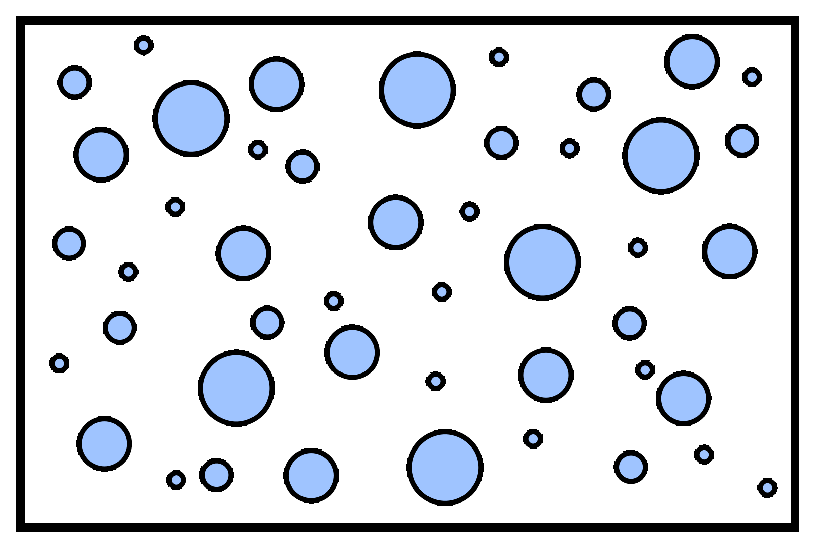
\includegraphics[width=0.5\textwidth]{fig/drawing/drawingDA.eps}
\end{center}
\caption{Sketch of a collection of particles deposited on a substrate whose scattering  could be described by the decoupling approximation.}
\label{fig:da}
\end{figure}


In concentrated systems, DA breaks down because of correlations. One solution is to reintroduce some correlations between particles sizes and distributions using, for example, the size spacing correlation approximation described below. 

\paragraph{Local monodisperse approximation (LMA)}
\index{Local monodisperse approximation}
partially accounts for some coupling between the positions and the kinds of the particles \cite{Ped94}. 
 It requires a subdivision of the layers of particles into monodisperse domains. The contributions of these subdomains are then  incoherently summed up and weighted by the size-shape probabilities.\\ In this approximation, a particle is supposed to be surrounded by particles of the same size and shape, within the coherence length of the input beam (see fig.~\ref{fig:lma}). The scattering cross-section is expressed as
\begin{equation*}
  \left\langle \frac{d\sigma}{d\Omega}(\vect{q}) \right\rangle \simeq \left\langle \left\lvert F_\alpha(\vect{q})\right\rvert ^2 S_\alpha(\vect{q}) \right\rangle_\alpha \; .
\end{equation*}

Contrary to the Decoupling Approximation, the Local Monodisperse Approximation can account for particle class/size/shape-dependent pair correlation functions by having distinct interference functions $S_\alpha(\vect{q})$.

One has to remember that in most cases, this approximation corresponds to an unphysical description of the investigated systems. \\ 

DA and LMA separate the contributions of the form factors and of the interference function. For disordered systems DA and LMA give the same result as the scattering vector gets larger \textit{i.e.} the scattered intensity is dominated by the contribution of the form factor.

\begin{figure}[ht]
\begin{center}
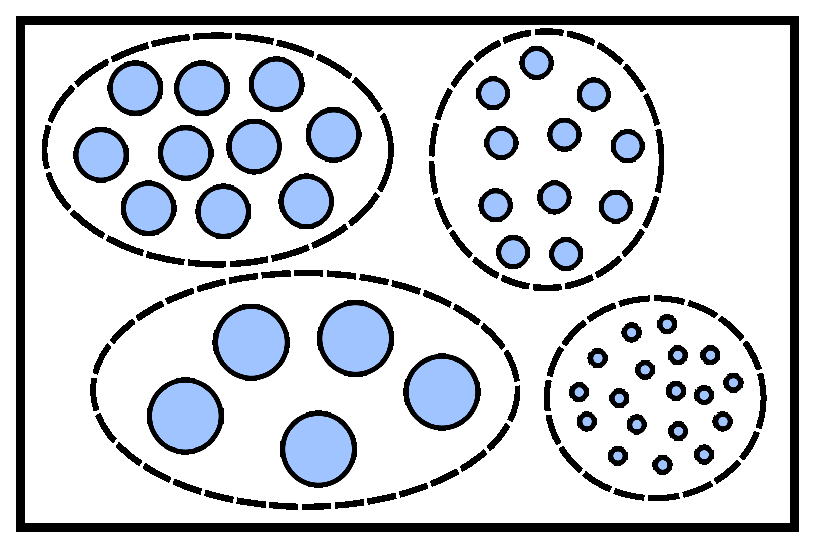
\includegraphics[width=0.5\textwidth]{fig/drawing/drawingLMA.eps}
\end{center}
\caption{Sketch of a collection of particles deposited on a substrate whose scattering could be described by the local monodisperse correlation approximation. The dashed areas mark the coherent domains. In this case, the total scattering intensity is the incoherent sum from all these domains.}
\label{fig:lma}
\end{figure}

\paragraph{Size spacing correlation approximation (SSCA)}
\index{Size-spacing correlation approximation}
introduces correlations between polydisperse particles, more precisely between the size of the particles and their mutual spacing. A classical example would consist in particles whose closest-neighbor spacing depends linearly on the sum of their respective sizes \cite{LaLR07}, as illustrated in fig.~\ref{fig:ssca}.

%For a sample where only the statistical properties of particle positions and size are known, the scattered intensity per scattering particle is expressed as the average over an ensemble of the Fourier transform of the Patterson function, which is the autocorrelation of the scattering length density $\curlp (\vectr ) \equiv \sum_{ij} S_i(-\vectr )\otimes S_j(\vectr )\otimes \delta (\vectr + \vectr_i - \vectr_j )$:
%\begin{equation*}
%  I(\vectq ) = \frac{1}{N}\ensavg{}{\curlf (\curlp (\vectr ))} \; ,
%\end{equation*}
%where $\curlf$ denotes the Fourier transform and $\curlp$ the Patterson function

\begin{figure}[ht]
\begin{center}
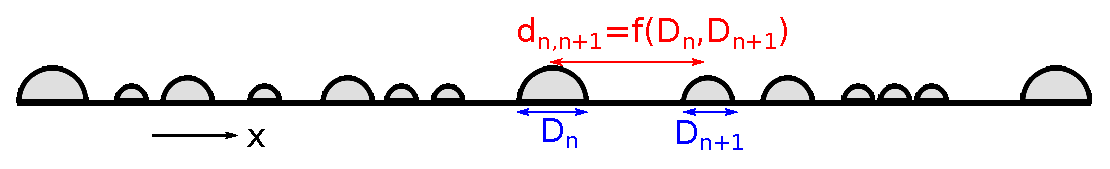
\includegraphics[width=0.9\textwidth]{fig/drawing/drawingSSCA.eps}
\end{center}
\caption{Sketch of a 1D distributed collection of particles, whose scattering could be described by the size-spacing correlation approximation: the distance between two particles depends on their sizes.}
\label{fig:ssca}
\end{figure}



\MakeRemark{Terminology}{
\\
For collections of particles, the scattered intensity contains contributions from neighboring particles. This additional pattern can be called the structure factor, the interference function or even in crystallography, the lattice factor. In this manual, we use the term "interference function" or interferences.
}


%===============================================================================
\subsection{Layout of particles}\label{sec:partlayout}
%===============================================================================

\subsubsection{The uncorrelated or disordered lattice}
For very diluted distributions of particles, the particles are too far apart from each other to lead to any interference between the waves scattered by each of them. In this case the interference function is equal to 1. The scattered intensity is then entirely determined by the form factors of the particles distributed in the sample.

\subsubsection{The regular  lattice}\mbox{}\\
The particles are positioned at regular intervals generating a layout characterized by its base vectors $\mathbf{a}$ and $\mathbf{b}$ (in direct space) and the angle between these two vectors.
This lattice can be two or one-dimensional depending on the characteristics of the particles. For example when they are infinitely long, the implementation can be simplified and reduced to a "pseudo" 1D system.

\paragraph{The ideal paracrystal} \mbox{}\\
\index{Paracrystal}
A paracrystal, whose notion was developed by Hosemann\cite{Hos51}, allows fluctuations of the lengths and orientations of lattice vectors. Paracrystals can be defined as distorted crystals in which the crystalline order has not disappeared and for which the behavior of the interference functions  at small angles is coherent.
It is a transition between the regular lattice and the disordered state.\\

For example, in one dimension, a paracrystal is generated using the following method. First we place a particle at the origin. The second particle is put at a distance $x$ with a density probability $p(x)$ that is peaked at a mean value $D$: $\int_{-\infty} ^{\infty}p(x)dx=1$ and $\int_{-\infty}^{\infty}xp(x)dx=D$. The third one is added at a distance $y$ from the second site using the same rule with a density probability $p_2(y)= \int_{-\infty}^{\infty}p(x)p(y-x)dx=p\otimes p(y)$.\\ With such a method, the pair correlation function $g(x)$ is built step by step. Its expression and the one of its Fourier transform, which is the interference function are 
\begin{equation*}
g(x)=\delta(x)+ p(x)+ p(x)\otimes p(x)+\ldots + p(-x)+\ldots \: \mathrm{and}\:\, S(q)=\Re\left(\dfrac{1+P(q)}{1-P(q)}\right),
\end{equation*}
 where $P(q)$ is the Fourier transform of the density probability $p(x)$.\\

\paragraph{Example} For a probability distribution function is Gaussian:
\begin{equation*}
p(x)=\frac{1}{\omega \sqrt{2\pi}} \exp\left(-\dfrac{(x-D)^2}{\omega^2}\right),\qquad P(q)=\exp\left(-\frac{q^2 \omega^2}{2}\right)\exp(iqD).
\end{equation*}
 The interference function of a one-dimensional paracrystal is given by

\begin{align*}
S(q) =\Re \left(\frac{1+\Phi(q) }{1 - \Phi(q)} \right), \quad \mathrm{where}\quad \Phi(q) = P(q)\exp\left(-\frac{D}{\Lambda}\right),
\end{align*}
where $\Lambda$ is a damping length used in order to introduce some finite-size effects.

Figure~\ref{fig:1dparas_q} shows the evolution of $S(q)$ for different values of $\omega /D$. 

\begin{figure}[ht]
\begin{center}
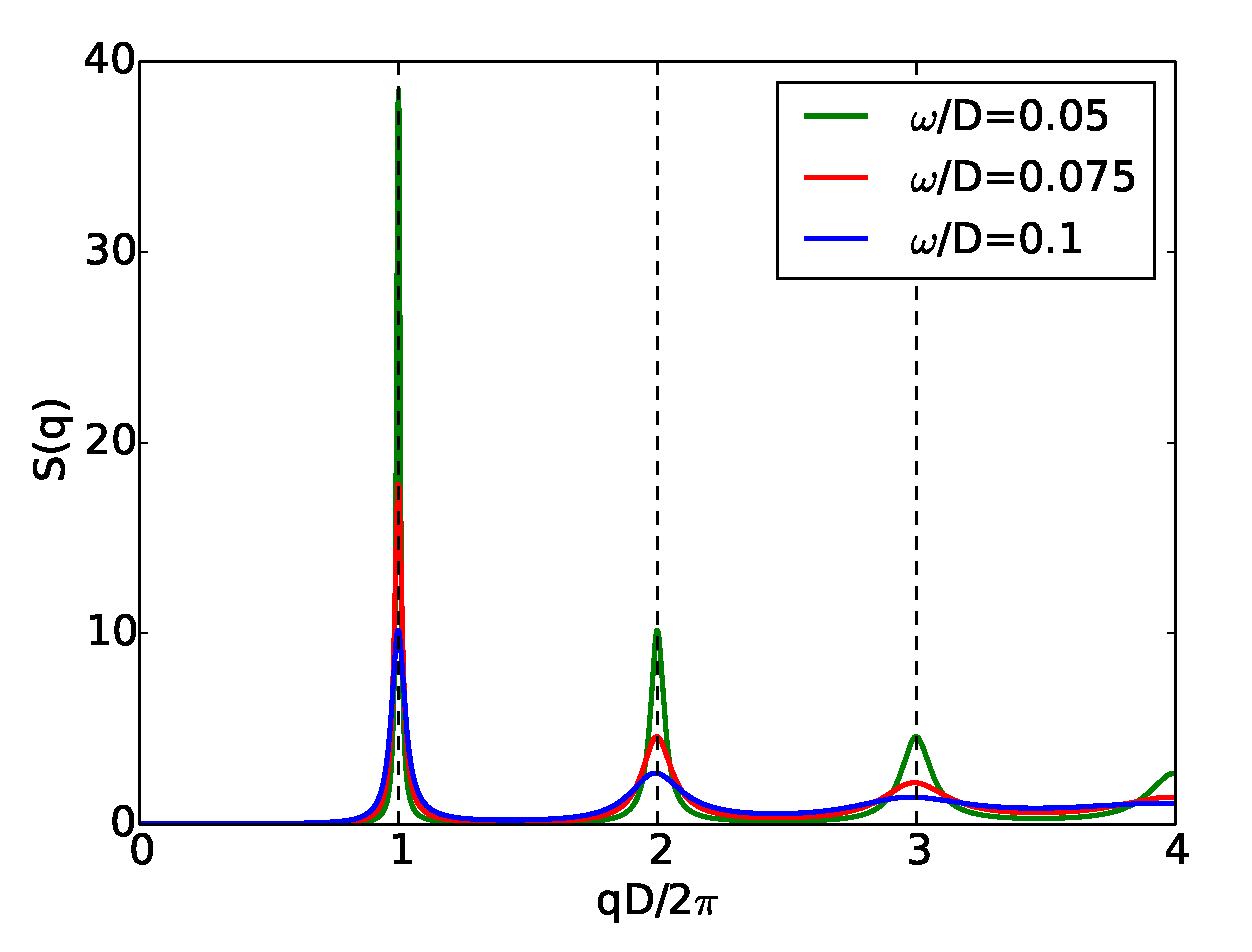
\includegraphics[width=0.6\textwidth]{fig/funcplot/S_q_1Dparacrystal.eps}
\end{center}
\caption{Interference function of a 1D Gaussian paracrystal plotted for different values of $\omega /D$. The peaks broaden with a decreasing amplitude as $\omega/D$ increases. This shows the transition between an ordered and a disordered states. }
\label{fig:1dparas_q}
\end{figure}

In two dimensions, the paracrystal is constructed on a pseudo-regular lattice with base vectors $\mathbf{a}$ and $\mathbf{b}$ using the following conditions for the densities of probabilities:\\ $\int p_{\mathbf{a}}(\mathbf{r})d^2\mathbf{r}=\int p_{\mathbf{b}}(\mathbf{r})d^2\mathbf{r}=1$, $\int \mathbf{r} p_{\mathbf{a}}(\mathbf{r})d^2\mathbf{r}=\mathbf{a}$, $\int \mathbf{r} p_{\mathbf{b}}(\mathbf{r})d^2\mathbf{r}=\mathbf{b}$.\\
In the ideal case the deformations along the two axes are decoupled and each unit cell should retain a parallelogram shape. The interference function is given by\\ $S(q_{\parallel})=\prod_{k=a,b}\Re\left(\dfrac{1+P_k(q_{\parallel})}{1-P_k(q_{\parallel})} \right)$ with $P_k$ the Fourier transform of $p_k$, $k=a, b$.

\paragraph{Probability distributions} \mbox{}\\
The scattering by an ordered lattice gives rise to a series of Bragg peaks situated at the nodes of the reciprocal lattice. Any divergence from the ideal crystalline case modifies the output spectrum by, for example, widening or attenuating the Bragg peaks. The influence of these "defects" can be accounted for 
 in direct space by using correlation functions or by truncating the lattice or, in reciprocal space with structure factors or interference functions by convoluting the scattered peaks with a function which could reproduce the experimental shapes.


%===============================================================================
\subsubsection{General formulas}
%===============================================================================

Even in the most general case, the partial pair correlation function will only depend on the difference $\vect{R}_{\alpha\beta}\equiv(\vect{R}_\alpha - \vect{R}_\beta )$ of the particles' positions. One of the volume integrals can then be dropped, together with the volume factor, giving:
\begin{align*}
  \left\langle \frac{d\sigma}{d\Omega}(\vect{q}) \right\rangle  & = \sum_\alpha p_\alpha \left\lvert F_\alpha(\vect{q})\right\rvert ^2 + \rho_V\sum_{\alpha,\beta} p_\alpha p_\beta F_\alpha (\vect{q})F_\beta^*(\vect{q}) \\
  & \times \int_V d^3\vect{R}_{\alpha\beta} \ppcfb{\alpha}{\beta}{R} \exp \left[ i\vect{q}\cdot \vect{R}_{\alpha\beta} \right] \; .
\end{align*}

This expression can be split into a diffuse part, which by definition should be zero for the case of only one particle type, and a coherent part, resulting from the coherent superposition of scattering amplitudes for particles at different positions:
\begin{equation*}
  \left\langle \frac{d\sigma}{d\Omega}(\vect{q}) \right\rangle = I_d(\vect{q}) + \ensavg{\alpha\beta}{F_\alpha (\vect{q} ) S_{\alpha\beta} (\vect{q}) F_\beta^* (\vect{q})} \; ,
\end{equation*}
where
\begin{align*}
  I_d(\vect{q}) &\equiv \ensavg{\alpha}{\left\rvert F_\alpha (\vect{q}) \right\rvert^2} - \left\lvert \ensavg{\alpha}{ F_\alpha (\vect{q})} \right\rvert^2 \; , \\
  S_{\alpha\beta} (\vect{q}) &\equiv 1 + \rho_V \int_V d^3\vect{R}_{\alpha\beta}\ppcfb{\alpha}{\beta}{R} \exp \left[ i\vect{q}\cdot \vect{R}_{\alpha\beta} \right] \; .
\end{align*}
$S_{\alpha\beta} (\vect{q})$ is called the \emph{interference function} and $\langle\dotso\rangle_\alpha$ is the expectation value over the classes $\lbrace \alpha\rbrace$.


%===============================================================================
\subsubsection{Decoupling approximation}
%===============================================================================
\index{Decoupling approximation}

When the partial pair correlation function is independent of the particle class $\alpha$ ($ \ppcfb{\alpha}{\beta}{R} \equiv g(\vect{R}_{\alpha\beta})$ ), the scattering cross-section becomes:
\begin{equation*}
\left\langle \frac{d\sigma}{d\Omega}(\vect{q}) \right\rangle  = I_d(\vect{q}) + \left\lvert \left\langle F_\alpha(\vect{q}) \right\rangle_\alpha \right\rvert ^2 \times S(\vect{q}) \; ,
\end{equation*}
where
\begin{equation*} 
  S(\vect{q}) = 1+ \rho_V \int_V d^3\vect{R} \; g(\vect{R}) \exp \left[ i\vect{q}\cdot \vect{R} \right] \; .
\end{equation*}


%===============================================================================
\subsubsection{Local Monodisperse Approximation}
%===============================================================================
\index{LMA|see {Local monodisperse approximation}}
\index{Local monodisperse approximation}
  
By assuming that inside every coherence region of the beam, the particle class (or size/shape) is fixed, the cross-section will consist of an incoherent superposition of these different coherence regions and can be written as:
\begin{equation*}
  \left\langle \frac{d\sigma}{d\Omega}(\vect{q}) \right\rangle \simeq \left\langle \left\lvert F_\alpha(\vect{q})\right\rvert ^2 S_\alpha(\vect{q}) \right\rangle_\alpha \; .
\end{equation*}

Contrary to the Decoupling Approximation, the Local Monodisperse Approximation can account for particle class/size/shape-dependent pair correlation functions by having distinct interference functions $S_\alpha(\vect{q})$.


%===============================================================================
\subsubsection{Size-Spacing Correlation Approximation}
%===============================================================================
\index{Size-spacing correlation approximation}
\index{SSCA|see {Size-spacing correlation approximation}}

In the Size-Spacing Correlation Approximation, a correlation is assumed between the shape/size of the particles and their mutual spacing. A classical example would consist of particles whose closest-neighbor spacing depends linearly on the sum of their respective sizes. The following discussion of this type of correlation is inspired by \cite{LaLR07}

The scattered intensity can also be calculated as the Fourier transform of the Patterson function, which is the autocorrelation of the scattering length density:
\begin{equation*}
  \curlp (\vectr ) \equiv \sum_{ij} S_i(-\vectr )\otimes S_j(\vectr )\otimes \delta (\vectr + \vectr_i - \vectr_j ) \; .
\end{equation*}
For a sample where only the statistical properties of particle positions and shape/size are known, the scattered intensity per scattering particle becomes average over an ensemble of the Fourier transform of the Patterson function:
\begin{equation*}
  I(\vectq ) = \frac{1}{N}\ensavg{}{\curlf (\curlp (\vectr ))} \; ,
\end{equation*}
where $\curlf$ denotes the Fourier transform.

The ensemble averaged Patterson function will be denoted as:
\begin{equation*}
  Z(r) \equiv \frac{1}{N}\ensavg{}{\curlp (\vectr )} \; .
\end{equation*}
In the case of systems where the particles are aligned in one dimension, this autocorrelation function can be further split into nearest neighbor probabilities. First, it is split into terms for negative, zero or positive distance:
\begin{equation*}
  Z(\vectr ) \equiv z_0(\vectr ) + z_+(\vectr ) + z_-(\vectr ) \; .
\end{equation*}
Taking $x$ as the coordinate in the direction in which the particles are arranged and $s$ as an orthogonal coordinate ($\vectr \equiv (x,s)$), one obtains:
\begin{align*}
  z_0(\vectr ) &= \sum_{\alpha_0} p(\alpha_0) S_{\alpha_0}(-x,-s) \otimes S_{\alpha_0}(x,s)  \\
  z_+(\vectr ) &= \sum_{\alpha_0\alpha_1} p(\alpha_0,\alpha_1) S_{\alpha_0}(-x,-s) \otimes S_{\alpha_1}(x,s) \otimes P_1(x|\alpha_0\alpha_1)  \\
               &+ \sum_{\alpha_0\alpha_1\alpha_2} p(\alpha_0,\alpha_1,\alpha_2) S_{\alpha_0}(-x,-s) \otimes S_{\alpha_2}(x,s) \otimes P_1(x|\alpha_0\alpha_1) \otimes P_2(x|\alpha_0\alpha_1\alpha_2)  \\
               &+ \dotsb \\
  z_-(\vectr ) &= z_+(-\vectr ) \; ,
\end{align*}
where $p(\alpha_0,\dotsc ,\alpha_n)$ denotes the probability of having a sequence of particles of the indicated sizes/shapes and $P_n(x|\alpha_0\dotsc\alpha_n)$ is the probability density of having a particle of type $\alpha_n$ at a (positive) distance $x$ of its nearest neighbor of type $\alpha_{n-1}$ in a sequence of the given order.

In the Size-Spacing Correlation Approximation, one assumes that the particle sequence probabilities are just a product of their individual fractions:
\begin{equation*}
  p(\alpha_0,\dotsc ,\alpha_n) = \prod_i p(\alpha_i) \; ,
\end{equation*}
and the nearest neighbor distance distribution is dependent only on the two particles involved:
\begin{equation*}
  P_n(x|\alpha_0\dotsc\alpha_n) = P_1(x|\alpha_{n-1}\alpha_n) \; .
\end{equation*}
Furthermore, the distance distribution $P_1(x|\alpha_0\alpha_1)$ depends on the particle sizes/shapes only through its mean value $D$:
\begin{equation*}
  P_1(x|\alpha_0\alpha_1) = P_0(x - D(\alpha_0,\alpha_1) ) \; ,
\end{equation*}
where $D(\alpha_0,\alpha_1) = D_0 + \kappa \left[ \Delta R(\alpha_0) + \Delta R(\alpha_1) \right]$, with $\Delta R(\alpha_i)$ the deviation of a size parameter of particle $i$ with respect to the mean over all particles sizes/shapes and $\kappa$ the coupling parameter.

In momentum space, the sum of convolutions can be written as a geometric series, which can be exactly calculated to be:
\begin{equation}
\label{eq:sscainf}
  I(\vectq ) = \ensavg{\alpha}{\left| F_\alpha(\vectq ) \right| ^2} + 2 \Re \left\lbrace \widetilde{\curlf_\kappa}(\vectq )\widetilde{\curlf_\kappa^*}(\vectq ) \cdot \frac{\Omega_\kappa(\vectq )}{\tilde{p}_{2\kappa}(\vectq )\left[ 1 - \Omega_\kappa(\vectq )\right] } \right\rbrace \; ,
\end{equation}
with
\begin{align*}
  \tilde{p}_\kappa(\vectq ) &= \int d\alpha\; p(\alpha) e^{i\kappa q_x \Delta R(\alpha)}  \\
  \Omega_\kappa(\vectq ) &= \tilde{p}_{2\kappa}(\vectq ) \phi(\vectq) e^{i q_x D_0}  \\
  \widetilde{\curlf_\kappa}(\vectq ) &= \int d\alpha\; p(\alpha)F_\alpha (\vectq ) e^{i\kappa q_x \Delta R(\alpha)} \; ,
\end{align*}
and the Fourier transform of $P_1(x|\alpha_0\alpha_1)$ is
\begin{equation*}
  \curlp (\vectq ) = \phi (\vectq )e^{i q_x D_0} e^{i \kappa q_x \left[ \Delta R(\alpha_0) + \Delta R(\alpha_1) \right] } \; .
\end{equation*}

Using the result from the one-dimensional analysis, one can apply this formula ad hoc for distributions of particles in a plane, where the coordinate $x$ will now be replaced with $(x,y)$, while the $s$ coordinate encodes a position in the remaining orthogonal direction. One must be aware however that this constitutes a further approximation, since this type of correlation does not have a general solution in more than one dimension.

The intensity in \refeq{sscainf} will contain a Dirac delta function contribution, caused by taking an infinite sum of terms that are perfectly correlated at $\vectq = 0$. One can leverage this behaviour by multiplying the nearest neighbor distribution by a constant factor $e^{-D/\Lambda}$, which removes the division by zero in \refeq{sscainf}.
Another way of dealing with this infinity at $\vectq =0$ consists of taking only a finite number of terms, in which case the geometric series still has an analytic solution, but becomes a bit more cumbersome:
\begin{equation*}
\begin{split}
  I(\vectq ) &= \ensavg{\alpha}{\left| F_\alpha(\vectq ) \right| ^2} + 2 \Re \Biggl\lbrace \frac{1}{\tilde{p}_{2\kappa}(\vectq )}\widetilde{\curlf_\kappa}(\vectq )\widetilde{\curlf_\kappa^*}(\vectq ) \\
  & \times \left[ \left( 1 - \frac{1}{N}\right) \frac{\Omega_\kappa(\vectq )}{1 - \Omega_\kappa(\vectq ) } - \frac{1}{N}\frac{\Omega_\kappa^2(\vectq )\left( 1- \Omega_\kappa^{N-1}(\vectq )\right) }{\left( 1 - \Omega_\kappa(\vectq ) \right) ^2 } \right] \Biggr\rbrace \; .
\end{split}
\end{equation*}
This expression has a well-defined limit for $\Omega_\kappa(\vectq ) \rightarrow 1$ (when $\vectq \rightarrow 0$), namely:
\begin{equation*}
  \lim_{\vectq \rightarrow 0} I(\vectq ) = \ensavg{\alpha}{\left| F_\alpha(0 ) \right| ^2} + \left( N-1 \right) \left| \ensavg{\alpha}{F_\alpha(0 )} \right|^2 \; .
\end{equation*}


%===============================================================================
\subsection{Vertical location of particles}
%===============================================================================

 \ImportantPoint{Remark:}{The particles cannot sit in between layers. At most they can be sitting on any inner interfaces.}

%-------------------------------------------------------------------------------
\subsubsection{Particles deposited on a substrate}
%-------------------------------------------------------------------------------
%Substrate modified Born approximation
In this configuration, the particles are sitting on top of a substrate layer, in the air as shown in fig.~\ref{fig:SchemDWBA}. In the DWBA the expression of a form factor becomes 
\begin{align}
F_{\rm{DWBA}}(q_{\parallel}, k_{i,z}, k_{f,z}) &= F_{\rm{BA}}(q_{\parallel}, k_{i,z}-k_{f,z})+ R_i F_{\rm{BA}}(q_{\parallel}, -k_{i,z}-k_{f,z}) \nonumber \\
&+ R_f F_{\rm{BA}}(q_{\parallel}, k_{i,z}+k_{f,z}) + R_i R_f F_{\rm{BA}}(q_{\parallel},-k_{i,z}+k_{f,z}), \label{eq:dwbaair}
\end{align}
where $q_{\parallel}$ is the component of the scattering beam in the plane of the interface ($\vect{q}=\vect{k}_i-\vect{k}_f$), $k_{i,z}$ and $k_{f,z}$ are the z-component of the incident and scattered beam, respectively. $R_i$, $R_f$ are the reflection coefficients in incidence and reflection. They are defined as\\ $R=\dfrac{k_z+\sqrt{n_s^2k_0^2-|k_{\parallel}|^2}}{k_z-\sqrt{n_s^2 k_0^2-|k_{\parallel}|^2}}$, where $n_s=1-\delta_s +i \beta_s$ is the refractive index of the substrate, $k_0$ is the wavelength in vacuum ($2\pi /\lambda$), $k_z$ and $k_{\parallel}$ are the $z$-component and the in-plane component of $\vect{k}_i$ or $\vect{k}_f$. \\

\ImportantPoint{Remark:}{If the particles are sitting on a multilayered system, the expression of the form factor in the DWBA is obtained by replacing the Fresnel coefficient by the corresponding coefficients of the underlying layers \cite{Par54,BoWo99}.}

\vspace{18pt}

Figure~\ref{fig:SchemDWBA} illustrates the four scattering processes for a supported particle, taken into account in the DWBA. The first term of eq.~\ref{eq:dwbaair}  corresponds to the Born approximation. Each term of $F_{\rm{DWBA}}$ is weighted by a Fresnel coefficient. 

\begin{figure}[ht]
\begin{center}
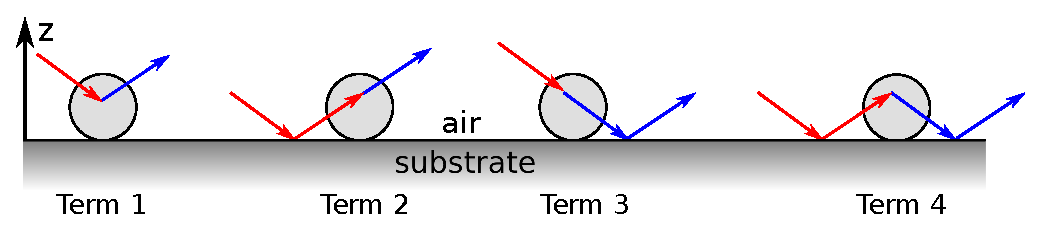
\includegraphics[width=\textwidth]{fig/drawing/drawingDWBA.eps}
\end{center}
\caption{Schematic views of the different terms appearing in the expression of the form factor under DWBA for particles sitting on a substrate layer.}
\label{fig:SchemDWBA}
\end{figure}


Script~\ref{lst:badwba} illustrates the difference between BA and DWBA in \BornAgain\ when generating the sample.  We consider the simple case of:
\begin{itemize}
\item one kind of particles' shape,
\item no interference between the particles,
\item in the DWBA, a sample made of a layer of substrate on which are deposited the particles,
\item in the BA, a sample composed of the particles in air.
\end{itemize} 

Figure~\ref{fig:spheroidbadwba} shows the intensity contour plot generated using this script with truncated spheroids as particles.

\newpage

\begin{lstlisting}[language=python, style=eclipseboxed,numbers=none,nolol,caption={\Code{Python} script to generate a sample using Born (BA) or Distorted Wave Born Approximation (DWBA). The difference between BA and DWBA in this simple case is the absence or presence of a substrate layer in the sample.},label={lst:badwba}]
def get_sample():
    """
    Build and return the sample to calculate form factor of 
    truncated spheroid in Born or Distorted Wave Born Approximation.
    """
    # defining materials
    m_ambience = HomogeneousMaterial("Air", 0.0, 0.0)
    m_substrate = HomogeneousMaterial("Substrate", 6e-6, 2e-8)
    m_particle = HomogeneousMaterial("Particle", 6e-4, 2e-8)

    # collection of particles
    ff= FormFactorTruncatedSpheroid(7.5*nanometer, 9.0*nanometer, 1.2)
    particleshape = Particle(m_particle, ff)
    particle_layout = ParticleLayout()
    particle_layout.addParticle(particleshape, 0.0, 1.0)

    # interferences
    interference = InterferenceFunctionNone()
    particle_layout.addInterferenceFunction(interference)

    # assembling the sample
    air_layer = Layer(m_ambience)
    air_layer.addLayout(particle_layout)
    substrate_layer = Layer(m_substrate, 0)

    multi_layer = MultiLayer()
    multi_layer.addLayer(air_layer)
    # Comment the following line out for Born Approximation
    multi_layer.addLayer(substrate_layer)
    return multi_layer
\end{lstlisting}


\begin{figure}[ht]
\hfill
\subfigure[Born Approximation]{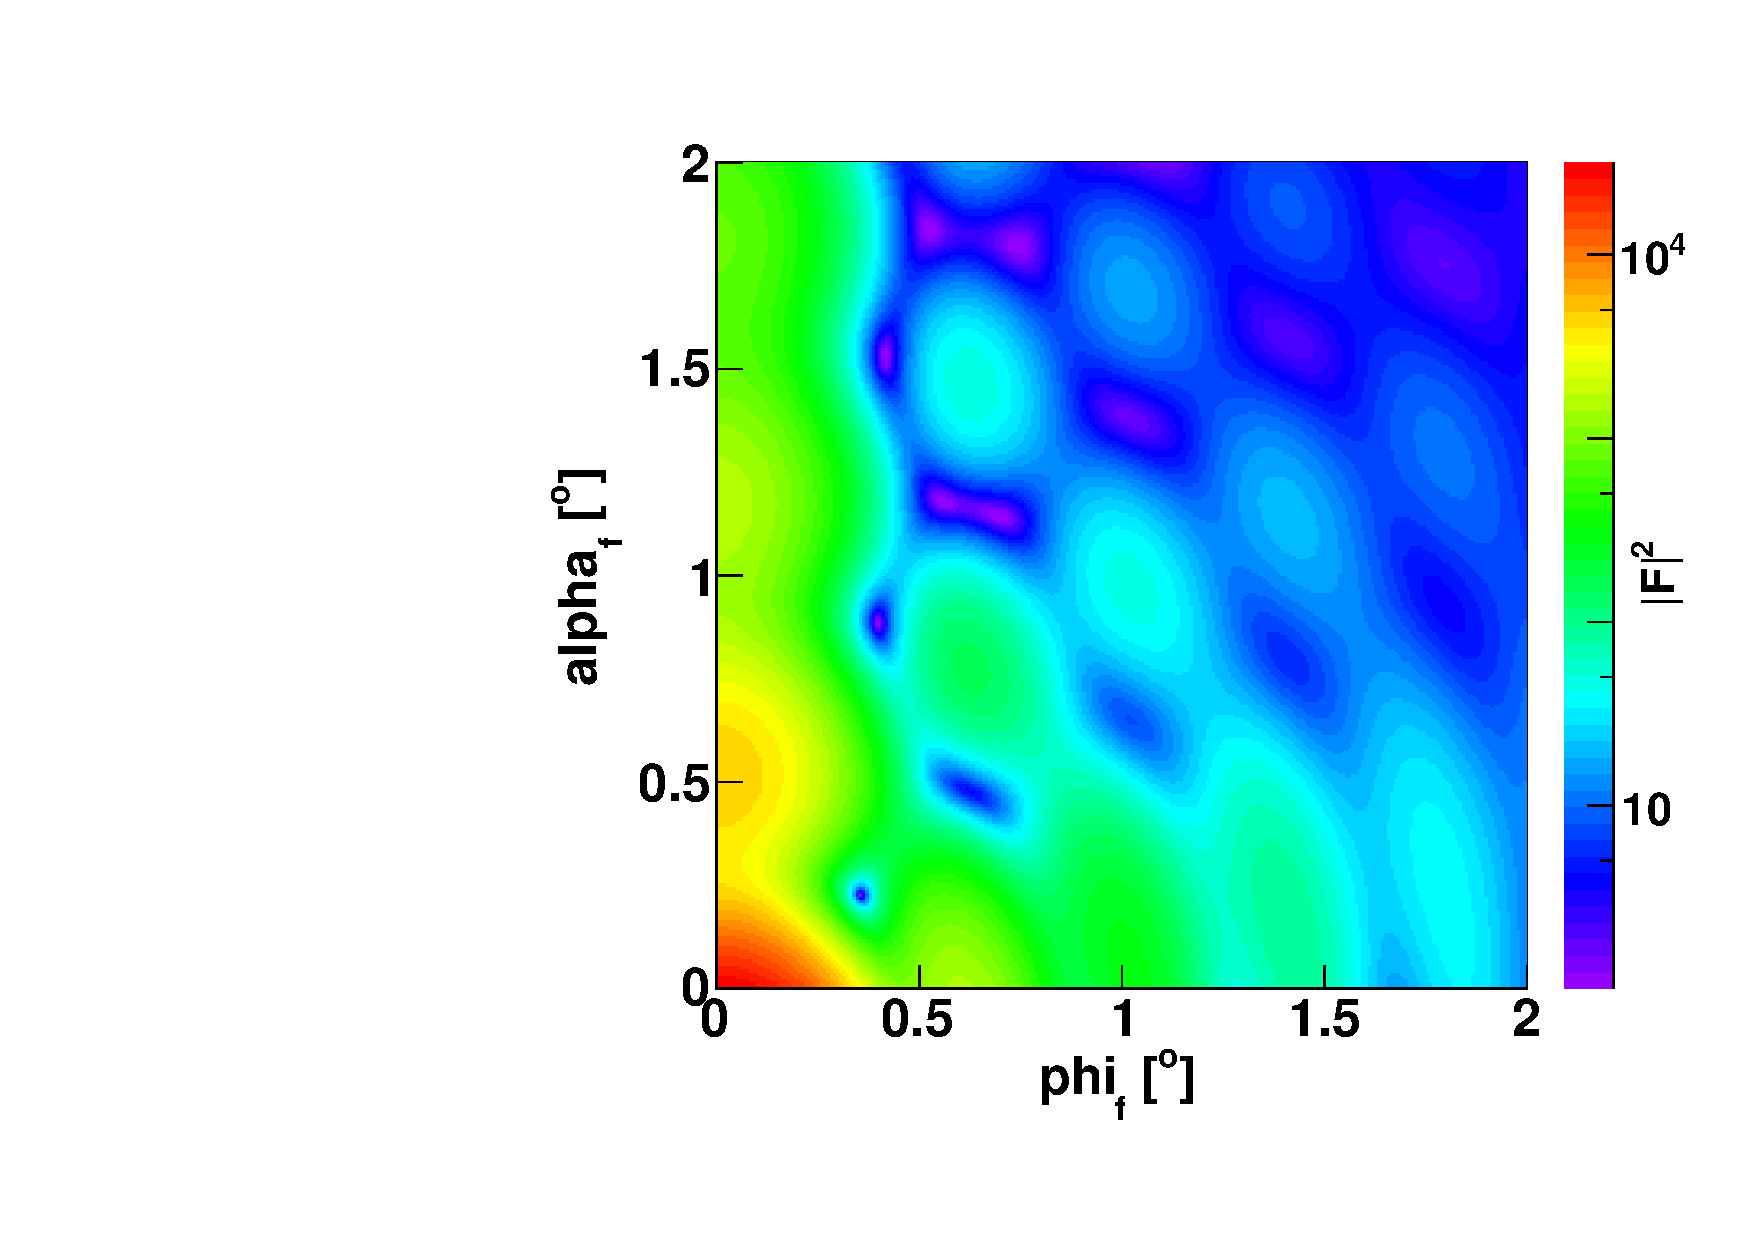
\includegraphics[angle=-90,width=6cm]{fig/gisasmap/ffspheroidBA.pdf}}
\hfill
\subfigure[DWB Approximation]{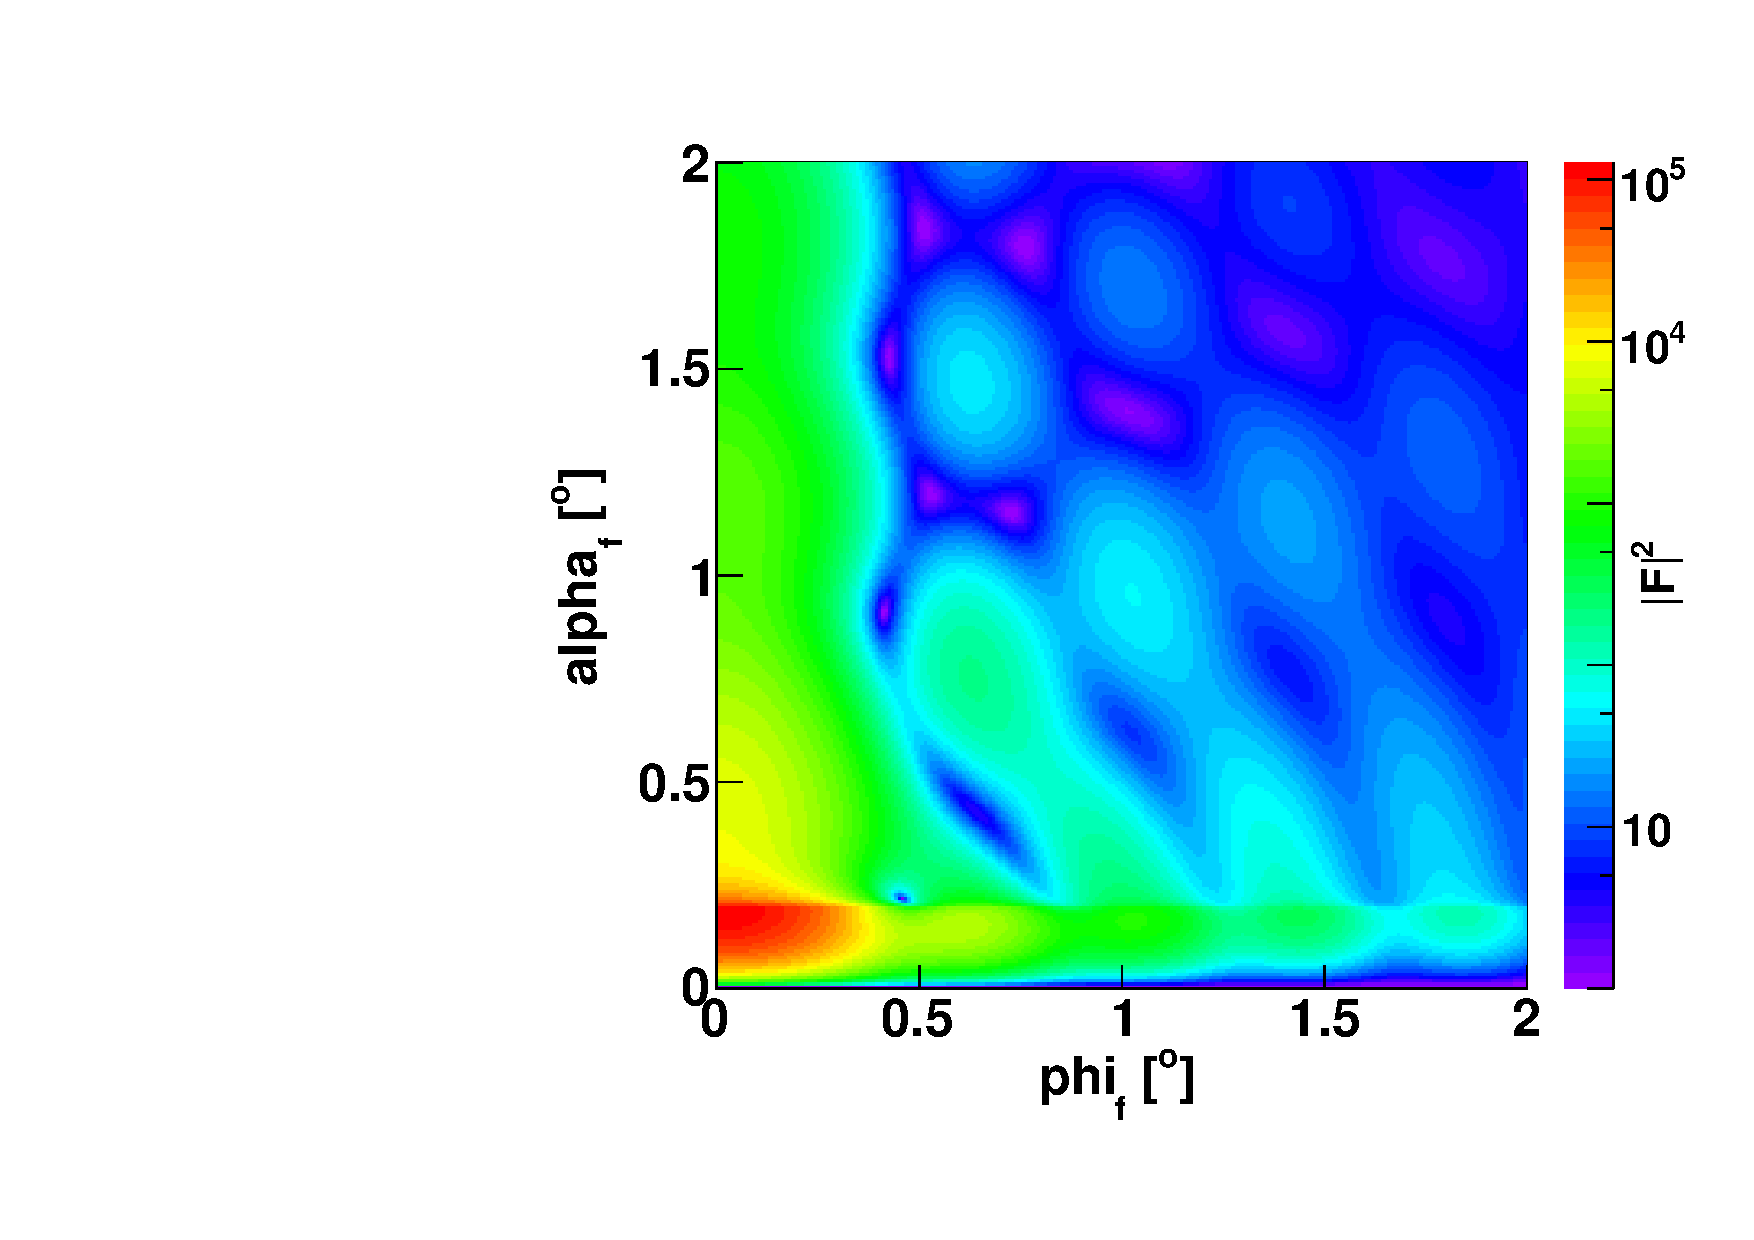
\includegraphics[angle=-90,width=6cm]{fig/gisasmap/ffspheroidDWBA.pdf}}
\hfill
\caption{Intensity map of TruncatedSpheroid form factor in BA and DWBA computing using script~\ref{lst:badwba} for the sample.}
\label{fig:spheroidbadwba}
\end{figure}

\FloatBarrier 

\ImportantPoint{Remark:}{In \BornAgain, the DWBA is implemented automatically when assembling the sample with more layers than only the air layer (for example, for particles are sitting on a substrate).}

%-------------------------------------------------------------------------------
\subsubsection{Buried particles} 
%-------------------------------------------------------------------------------

The system considered in this section consists of particles encapsulated in a layer, which is sitting on a substrate (see fig.~\ref{fig:SchemDWBAburied}). In this case the form factor in the DWBA is given by

\begin{align}
  F_{\rm{DWBA}}(q_{\parallel}, k_{i,z}, k_{f,z})
  &= T_i T_f F_{\rm{BA}}(q_{\parallel}, k_{i,z}-k_{f,z})e^{i(k_{i,z}-k_{f,z})d}\nonumber \\
  &+ R_i T_f F_{\rm{BA}}(q_{\parallel}, -k_{i,z}-k_{f,z})e^{i(-k_{i,z}-k_{f,z})d} \nonumber \\
  &+ R_f T_i F_{\rm{BA}}(q_{\parallel}, k_{i,z}+k_{f,z}) e^{i(k_{i,z}+k_{f,z})d}\nonumber \\
  &+ R_f R_iF_{\rm{BA}}(q_{\parallel},-k_{i,z}+k_{f,z})e^{i(-k_{i,z}+k_{f,z})d}, \label{eq:dwbaburied}
\end{align}

\begin{equation*}
R_j =\frac{t^{j}_{0,1}r^{j}_{1,2}\exp(2ik_{j,z}t)}{1+r^{j}_{0,1}r^{j}_{1,2}\exp(2ik_{j,z}t)}, \quad T_j=\frac{t^{j}_{0,1}}{1+r^{j}_{0,1}r^{j}_{1,2}\exp(2ik_{j,z}t)}, j=i,f 
\end{equation*}
where $q_{\parallel}$ is the component of the scattering beam in the plane of the interface, $k_{i,z}$ and $k_{f,z}$ are the z-component of the incident and scattered beams, respectively.  $d$ is the depth at which the particles are sitting in the layer. Note that this value is given relative to the top of this layer and it is not the coordinate in the absolute referential (linked with the full sample) and it is measured up to the bottom of the particle. $t$ is the thickness of the intermediate layer containing the particles. $R_{i,f}$ and $T_{i,f}$  are the reflection  and transmission coefficients in incidence and reflection (they can be calculated using Parratt or matrix formalism). $r^j_{0,1}$, $r^j_{1,2}$ $t^j_{0,1}$ are the reflection and transmission coefficients between layers; the indices are related to different boundaries with 0: air, 1: intermediate layer and 2: substrate layer and the superscript $j$ is associated with the incident or scattered beams:
\begin{equation*}
r^j_{n,n+1}=\frac{k_{j,z,n}-k_{j,z,n+1}}{k_{j,z,n}-k_{j,z,n+1}}, \qquad t^j_{n,n+1}= \frac{2k_{j,z,n}}{k_{j,z,n}-k_{j,z,n+1}}, \quad n=0,1, \quad j=i,f,
\end{equation*}
where index $n$ is related to the layers, $z$ to the vertical component, and $j$ to the beams (incident and outgoing).

\begin{figure}[ht]
\begin{center}
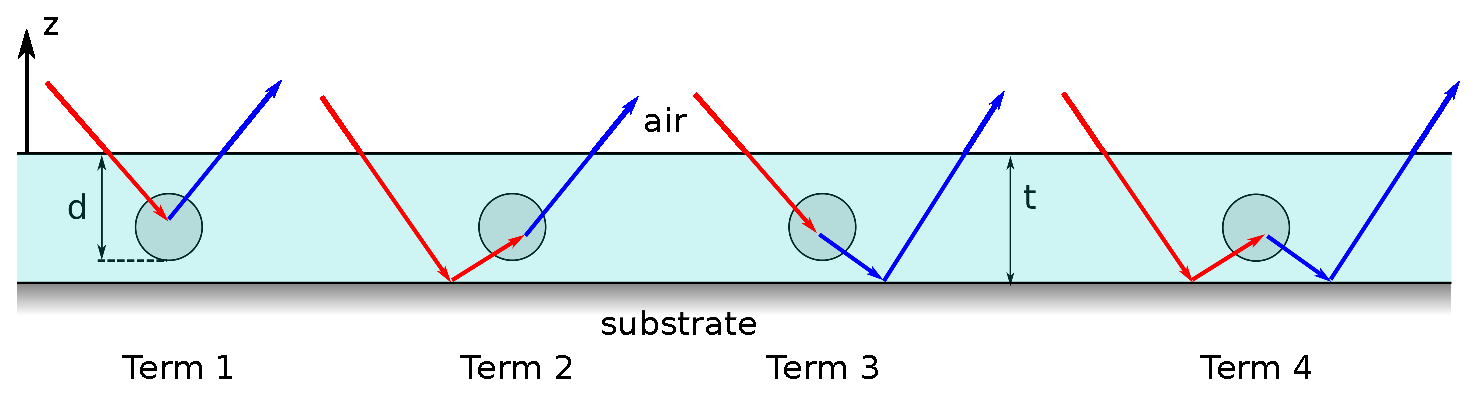
\includegraphics[width=\textwidth]{fig/drawing/drawingDWBAburied.eps}
\end{center}
\caption{Schematic views of the different terms appearing in the expression of the form factor under the DWBA for buried particles.}
\label{fig:SchemDWBAburied}
\end{figure}


Figure~\ref{fig:dwbaburied} shows a typical example of the output intensity scattered from a sample made of 3 layers: air, substrate, and in between, spherical particles embedded in the middle of a 30~nm-thick layer. This figure had been generated using listing~\ref{lst:dwbaburied}.

\begin{lstlisting}[language=python, style=eclipseboxed,numbers=none,nolol,caption={\Code{Python} script to generate a sample where spherical particles are embedded in the middle of a layer on a substrate.},label={lst:dwbaburied}]
def get_sample():
    """
    Build and return the sample with buried spheres in DWBA.
    """
    # defining materials
    m_ambience = HomogeneousMaterial("Air", 0.0, 0.0)
    m_interm_layer = HomogeneousMaterial("IntermLayer",3.45e-6, 5.24e-9)
    m_substrate = HomogeneousMaterial("Substrate", 7.43e-6, 1.72e-7)
    m_particle = HomogeneousMaterial("Particle", 0.0, 0.0)

    # collection of particles 
    ff = FormFactorFullSphere(10.2*nanometer)
    particleshape = Particle(m_particle, ff)
    particle_layout = ParticleLayout()
    particle_layout.addParticle(particleshape,25.2,1.0)

    # interferences 
    interference = InterferenceFunctionNone()
    particle_layout.addInterferenceFunction(interference)

    # assembling the sample 
    air_layer = Layer(m_ambience)
    intermediate_layer = Layer(m_interm_layer, 30.*nanometer)
    intermediate_layer.addLayout(particle_layout)
    substrate_layer = Layer(m_substrate, 0)
   
    multi_layer = MultiLayer()
    multi_layer.addLayer(air_layer)
    multi_layer.addLayer(intermediate_layer)
    multi_layer.addLayer(substrate_layer)
    return multi_layer
\end{lstlisting}


\begin{figure}[ht]
\centering
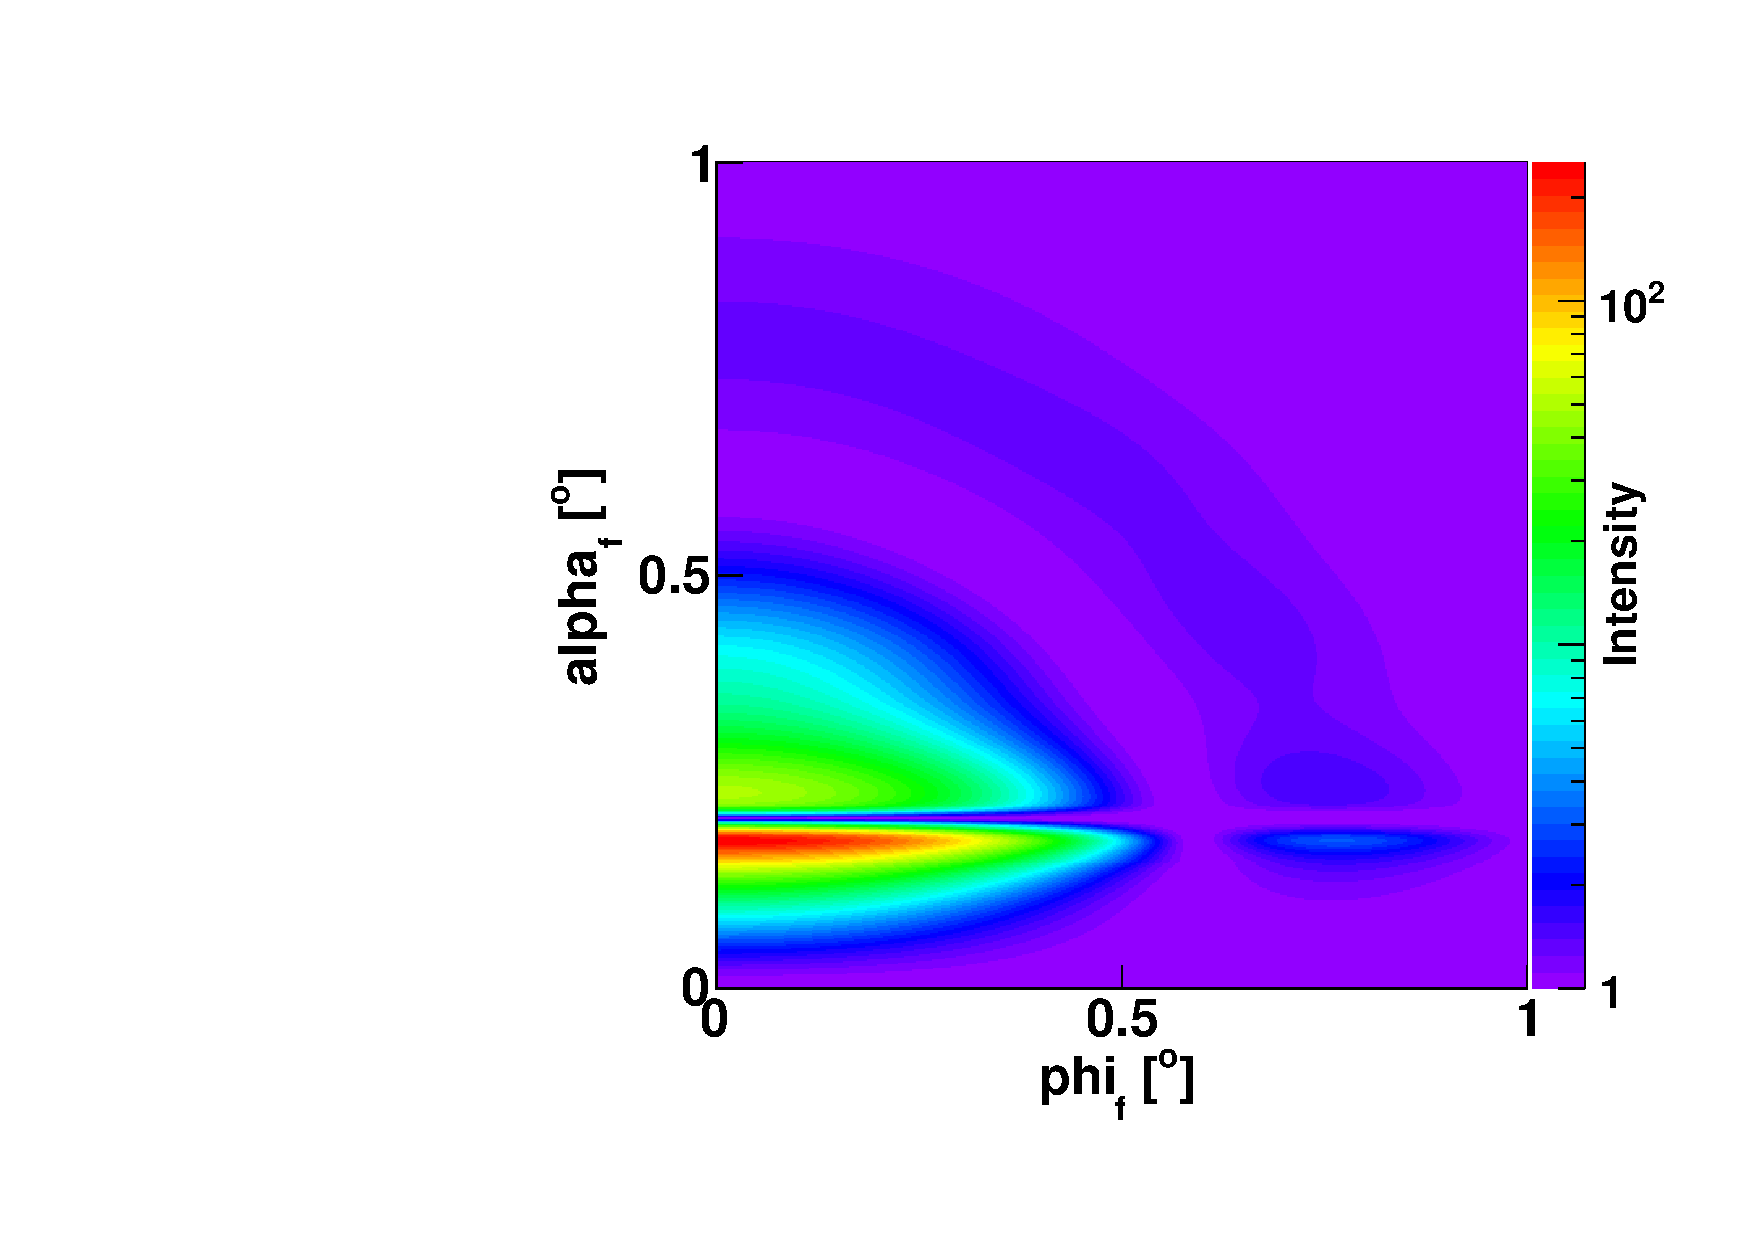
\includegraphics[angle=-90,width=0.6\textwidth]{fig/gisasmap/figIntBuriedPart.pdf}
\caption{Map of intensity scattered from a sample made of spherical particles embedded in the middle of a 30~nm-thick layer on a substrate (see Script~\ref{lst:dwbaburied} for details about the sample).}
\label{fig:dwbaburied}
\end{figure}

\newpage

\ImportantPoint{Remark:}{For layers different from the air layer, the top interface is considered as the reference level to position the encapsulated particles. For example, spheres positioned at depth $d$ (positive) are located at a distance $d$ from the top of the layer up to the bottom of these particles. This convention is different for the top air layer, where particles sitting at the interface with an underlying layer (\textit{i.e.} the bottom of the air layer) are located at depth 0 (see fig.~\ref{fig:depthpartBA}).}


\begin{figure}[ht]
\centering
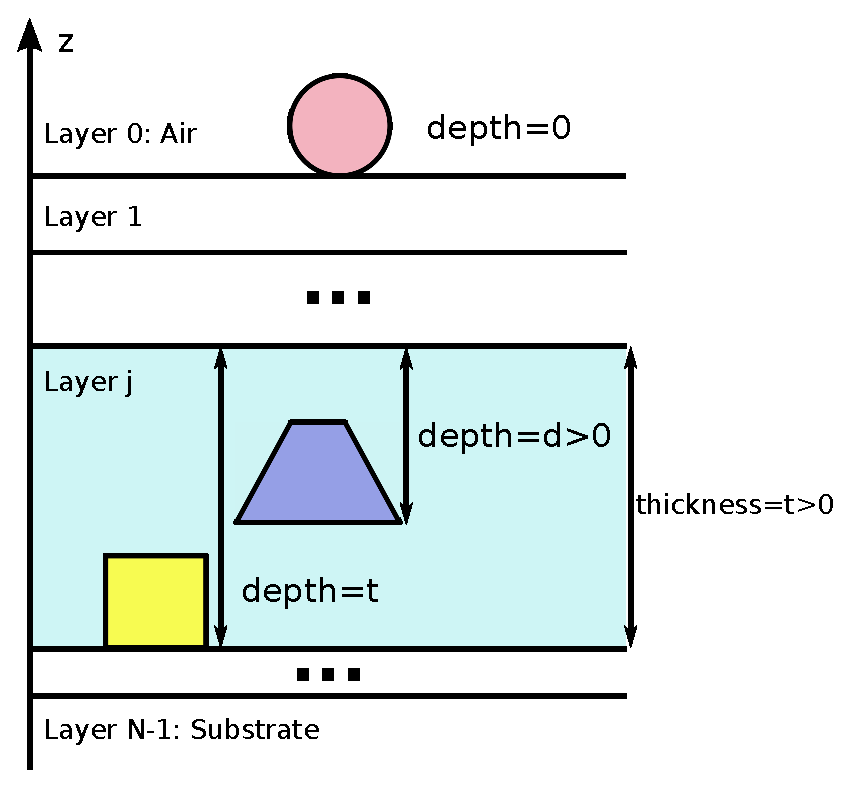
\includegraphics[width=0.5\textwidth]{fig/drawing/drawingDepthParticle.eps}
\caption{Illustration of the convention about \Code{depth} used in \BornAgain\ to encapsulate particles in layers.}
\label{fig:depthpartBA}
\end{figure}



%===============================================================================
\subsection{Implementation in \BornAgain}
%===============================================================================

This section describes the implementation of the interference functions in \BornAgain. For an implementation of all the components of a simulation, the use is referred, for example, to \SecRef{Example1Python}.\\


\ImportantPoint{Remark:}{In \BornAgain\ the particles are positioned in the same vertical layer.}

\subsubsection{Size-distribution models}
\index{Size-distribution models}
The decoupling approximation (DA), local monodisperse approximation (LMA) and size spacing correlation approximation (SSCA) can be used in \BornAgain.
The selection between DA and SSCA is made using\\ 
\Code{ILayout.setApproximation(EInterferenceFunction approximation)} when defining the characteristics of the way particles and interference functions are embedded in a layer.  For example,
\begin{lstlisting}[language=python, style=eclipseboxed,numbers=none,nolol]
    particle_layout = ParticleLayout()
   ....
# interference approx chosen between: DA (default) and SSCA
    particle_layout.setApproximation(ILayout.DA)
\end{lstlisting}

Note that with the SSCA, the users have to specify the coupling parameter $\kappa$ (with the function \Code{setKappa}), which should be a positive dimensionless value. $\kappa$ characterizes the influence of the neighboring particles' sizes on their distance. If $\kappa=0$, the SSCA reduces to the DA with a radial paracrystal for the interference function.\\

For the LMA, its implementation is automatically done when using more than one layout of particles:
\begin{lstlisting}[language=python, style=eclipseboxed,numbers=none,nolol]
    particle_layout0 = ParticleLayout()
    particle_layout1 = ParticleLayout()
   ....
# association of each particles' layout with materials, form factors
#... and with a material layer
    layer_a = Layer(m_material_a)
    layer_a.addLayout(particle_layout0)
    layer_a.addLayout(particle_layout1)
\end{lstlisting}

%%ADD EXPLANATION ABOUT LMA

%-------------------------------------------------------------------------------
\subsubsection{Probability distribution functions}\label{baftd}
%-------------------------------------------------------------------------------

The probability distribution functions have been implemented in the reciprocal space in \BornAgain. Their expressions are given in Table~\ref{table:pdf}.

\begin{table}[H]
\centering
\begin{tabular}{ccc}
\hline 
Function & One dimension & Two dimensions\\
\hline 
Cauchy & $(1+q^2\omega^2)^{-3/2}$ & $(1 + q_x^2 cl_x^2 + q_y^2 cl_y^2)^{-3/2}$ \\
Gauss & $\dfrac{1}{2}\exp(-\dfrac{q^2\omega^2}{4})$ & $\frac{1}{2}\exp\left(-\dfrac{q_x^2 cl_x^2+ q_y^2cl_y^2}{4}\right)$ \\
Voigt & $\dfrac{\eta}{2} \exp\left(-\dfrac{q^2\omega^2}{4}\right) + \dfrac{1 - \eta}{(1 + q^2\omega^2)^{3/2}}$ & $\dfrac{\eta}{2} \exp\left(-\dfrac{q_x^2 cl_x^2+ q_y^2cl_y^2}{4}\right)+ \dfrac{1 - \eta}{(1 + q_x^2 cl_x^2+ q_y^2cl_y^2)^{3/2}}$ \\
\hline
\end{tabular}
\caption{List of probability distribution functions in reciprocal space. $\omega$, $cl$ stand for coherence lengths (the index refers to the axis) and  $\eta$ is a weighting coefficient.}
\label{table:pdf}
\end{table}

The Cauchy distribution corresponds to $\exp(-r)$ in real space and the Voigt one  is a linear combination of the Gaussian and Cauchy probability distribution functions.\\

\noindent \underline{One dimension}
\begin{itemize}
\item \Code{FTDistribution1DCauchy($\omega$)},
\item \Code{FTDistribution1DGauss($\omega$)},
\item \Code{FTDistribution1DVoigt($\omega, \eta$)}.
\end{itemize}
where $\omega$ is the coherence length and $\eta$ is a weighting factor.\\

\noindent \underline{Two dimensions}
\begin{itemize}
\item \Code{FTDistribution2DCauchy($cl_x$, $cl_y$)},
\item \Code{FTDistribution2DGauss($cl_x$, $cl_y$)},
\item \Code{FTDistribution2DVoigt($cl_x$, $cl_y$)}
\end{itemize}
where $cl_{x,y}$ are the coherence lengths in the $x$ or $y$ direction, respectively.

These functions can be used with all interference functions, except the case without any interference.

%-------------------------------------------------------------------------------
\subsubsection{Interferences}
%-------------------------------------------------------------------------------
\index{Interference function}

The interference function is specified when building the sample. It is linked with the particles (shape, material). Examples of implementation are given at the end of each description.

\paragraph{Syntax:}
 \Code{particle\_layout.addInterferenceFunction(interference\_function)},\\ where \Code{particle\_layout} holds the information about the different shapes and their proportions for a given layer of particles, and \Code{interference\_function}  is one of the following expressions:
\begin{itemize}
\item \Code{InterferenceFunctionNone()}
\item \Code{InterferenceFunction1DLattice(lattice\_parameters)}
\item \Code{InterferenceFunctionRadialParaCrystal(peak\_distance, damping\_length)}
\item \Code{InterferenceFunction2DLattice(lattice\_parameters)}
\item \Code{InterferenceFunction2DParaCrystal(length\_1, length\_2, $\alpha$\_lattice, $\xi$, \\ damping\_length)}
\end{itemize}

\ImportantPoint{Remark:}{\Code{InterferenceFunction1DLattice} can only be used for particles which are infinitely long in one direction of the sample's surface like for example a rectangular grating.}

\newpage
%-------------------------------------------------------------------------------
\subsubsection{\ding{253} \Code{InterferenceFunctionNone()}} 
%-------------------------------------------------------------------------------

The particles are placed randomly in the dilute limit and are considered as individual, non-interacting scatterers. The scattered intensity is function of the form factors only. 

\paragraph{Example} The sample is made of a substrate on which are deposited half-spheres. Script~\ref{lst:nointerf} details the commands necessary to generate such a sample. Figure~\ref{fig:nointerf} shows an example of output intensity: Script~\ref{lst:nointerf}  + detector's + input beam's characterizations.


\begin{figure}[ht]
\begin{center}
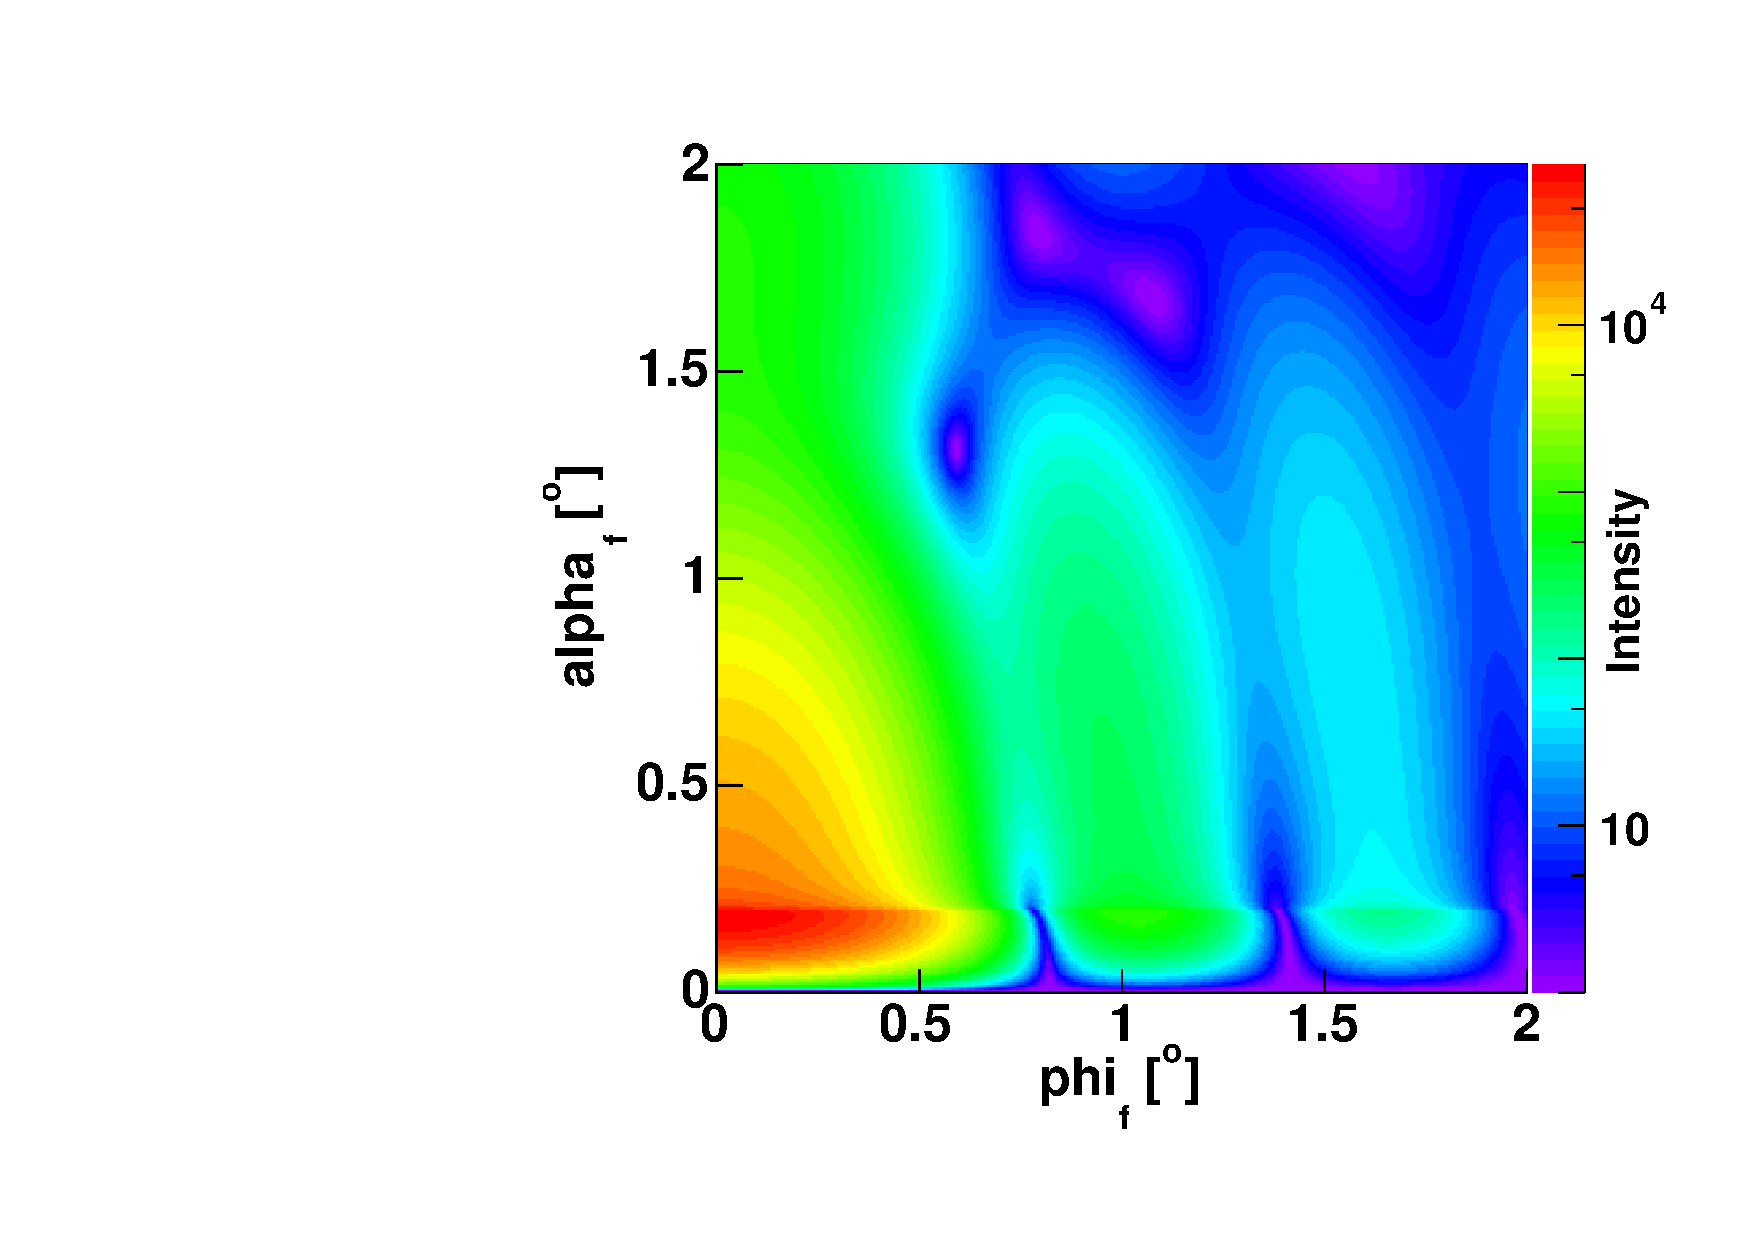
\includegraphics[angle=-90,width=0.5\textwidth]{fig/gisasmap/HSphere_NoInterf.pdf}
\end{center}
\caption{Output intensity scattered from a sample made of half-spheres with no interference between them.}
\label{fig:nointerf}
\end{figure}

\FloatBarrier
\newpage

\begin{lstlisting}[language=python, style=eclipseboxed,numbers=none,nolol,caption={\Code{Python} script to simulate a sample made of half-spheres deposited on a substrate layer without any interference. The part specific to the interferences is marked in a red italic font.},label={lst:nointerf}]
def get_sample():
    """
    Build and return the sample representing particles with no interference
    """
    # defining materials
    m_ambience = HomogeneousMaterial("Air", 0.0, 0.0)
    m_substrate = HomogeneousMaterial("Substrate", 6e-6, 2e-8)
    m_particle = HomogeneousMaterial("Particle", 6e-4, 2e-8)
    # collection of particles
    sphere_ff = FormFactorTruncatedSphere(5*nanometer, 5*nanometer)
    sphere = Particle(m_particle, sphere_ff)
    particle_layout = ParticleLayout()
    particle_layout.addParticle(sphere, 0.0, 1.0)
    |interference = InterferenceFunctionNone()| 
    |particle_layout.addInterferenceFunction(interference)|
    # assembling the sample
    air_layer = Layer(m_ambience)
    air_layer.addLayout(particle_layout)
    substrate_layer = Layer(m_substrate, 0)

    multi_layer = MultiLayer()
    multi_layer.addLayer(air_layer)
    multi_layer.addLayer(substrate_layer)
    return multi_layer
\end{lstlisting}

\newpage
%-------------------------------------------------------------------------------
\subsubsection{\ding{253}  \Code{InterferenceFunction1DLattice(lattice\_length, xi)}} 
%-------------------------------------------------------------------------------
where lattice\_length is the lattice constant and $\xi$ the angle in radian between the lattice unit vector and the $\mathbf{x}$-axis of the reference Cartesian frame as shown in fig.~\ref{fig:1dgrating}.

\begin{figure}[ht]
\begin{center}
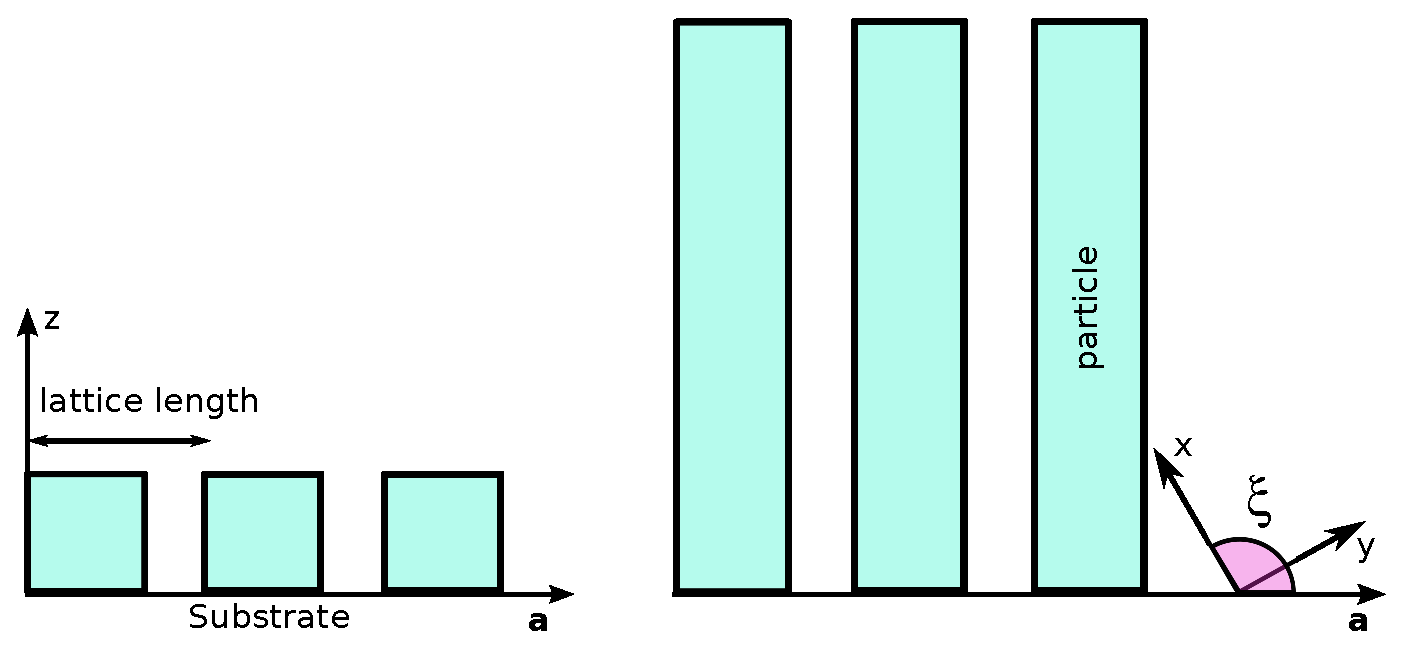
\includegraphics[width=0.75\textwidth]{fig/drawing/1DGrating.eps}
\end{center}
\caption{Schematic representation of a 1D lattice (side and top views). Such a lattice is characterized by a lattice length and the angle $\xi$.}
\label{fig:1dgrating}
\end{figure}

\ImportantPoint{Remark:}{By default the long axis of the particles in this 1D lattice is along the beam axis. That is the reason why in the example below the particles are rotated by  $90^{\circ}$ in the $(x,y)$ plane: the main axis of the lattice is therefore parallel to the y-axis, perpendicular to the long axis of the particles.}

\vspace{12pt}
A probability distribution function \Code{pdf} has to be chosen from the list in section~\ref{baftd} in order to apply some modifications to the scattering peaks. This function is implemented using \Code{setProbabilityDistribution(pdf)}. 

\paragraph{Example:} Script~\ref{lst:1dlattinterf} details how to build in  \BornAgain\ a sample using\\ \Code{InterferenceFunction1DLattice} as the interference function. As mentioned previously, this interference function can only be used with infinitely wide or long particles.\\ Here the sample is made of infinitely long boxes deposited on a substrate (these particles are characterized by their widths and heights). They are also rotated by $90^{\circ}$  in the sample surface in order to have their long axis perpendicular to the input beam, which is along the $x$-axis.\\
 The lattice parameters (the lattice length and angle between the lattice main axis and the $x$-axis) are passed into the constructor of the interference function.

\newpage
\begin{lstlisting}[language=python, style=eclipseboxed,numbers=none,nolol,caption={\Code{Python} script to generate a sample made of infinitely long boxes deposited on a substrate layer with the 1DLatticeInterference function. The part specific to the interferences is marked in a red italic font.},label={lst:1dlattinterf}]
def get_sample():
    """
    Build and return the sample with 1DLatticeInterference function
    """
    # defining materials
    m_air = HomogeneousMaterial("Air", 0.0, 0.0)
    m_substrate = HomogeneousMaterial("Substrate", 6e-6, 2e-8)
    m_particle = HomogeneousMaterial("Particle", 6e-4, 2e-8)

    # collection of particles
    ff = FormFactorInfLongBox(10.*nanometer, 15.0*nanometer)
    box = Particle(m_particle, ff)
    particle_layout = ParticleLayout()
    transform = Transform3D.createRotateZ(90.0*degree)
    particle_layout.addParticle(box, transform)

    # interference function
    |interference = InterferenceFunction1DLattice(30.0*nanometer, 0.0*degree)|
    |pdf = FTDistribution1DCauchy(200./2./M_PI*nanometer)|
    |interference.setProbabilityDistribution(pdf)|
    |particle_layout.addInterferenceFunction(interference)|

    # air layer with particles and substrate form multi layer
    air_layer = Layer(m_air)
    air_layer.addLayout(particle_layout)
    substrate_layer = Layer(m_substrate, 0)

    multi_layer = MultiLayer()
    multi_layer.addLayer(air_layer)
    multi_layer.addLayer(substrate_layer)
    return multi_layer
\end{lstlisting} 

\newpage
%-------------------------------------------------------------------------------
\subsubsection{\ding{253} \Code{InterferenceFunctionRadialParaCrystal(peak\_distance, damping\_length)}}  
%-------------------------------------------------------------------------------
\begin{itemize}
\item[where] \Code{peak\_distance} is the average distance to the first neighbor peak, 
\item[]\Code{width} is the width parameter of the probability distribution,
\item[] \Code{damping\_length} is used to introduce finite size effects by applying a multiplicative coefficient equal to  $\exp$(-\Code{peak\_distance/damping\_length}) to the Fourier transform of the probability densities. \Code{damping\_length} is equal to 0 by default and, in this case, no correction is applied.
\end{itemize}

A probability distribution function \Code{pdf} has to be chosen from the list in section~\ref{baftd} in order to apply some modifications to the scattering peaks. This function is implemented using \Code{setProbabilityDistribution(pdf)}. 


\MakeRemark{Remark}{
This interference function is not one-dimensional.  It takes into account the radial component of the scattering vector.
}

\paragraph{Example}
To illustrate the radial paracrystal interference function, we use the same sample as in the case without interference: half-spheres deposited on a substrate.

\begin{lstlisting}[language=python, style=eclipseboxed,numbers=none,nolol,caption={\Code{Python} script to define the radial paracrystal interference function between half-spheres, where \Code{trsphere} is of type \Code{Particle}.},label={lst:1dpara}]
    particle_layout = ParticleLayout()
    particle_layout.addParticle(trsphere, 0.0, 1.0)
    interference = InterferenceFunctionRadialParaCrystal(25.0*nanometer, 1e3*nanometer)
    pdf = FTDistribution1DGauss(7 * nanometer)
    interference.setProbabilityDistribution(pdf)
    particle_layout.addInterferenceFunction(interference)
\end{lstlisting}



\begin{figure}[ht]
\begin{center}
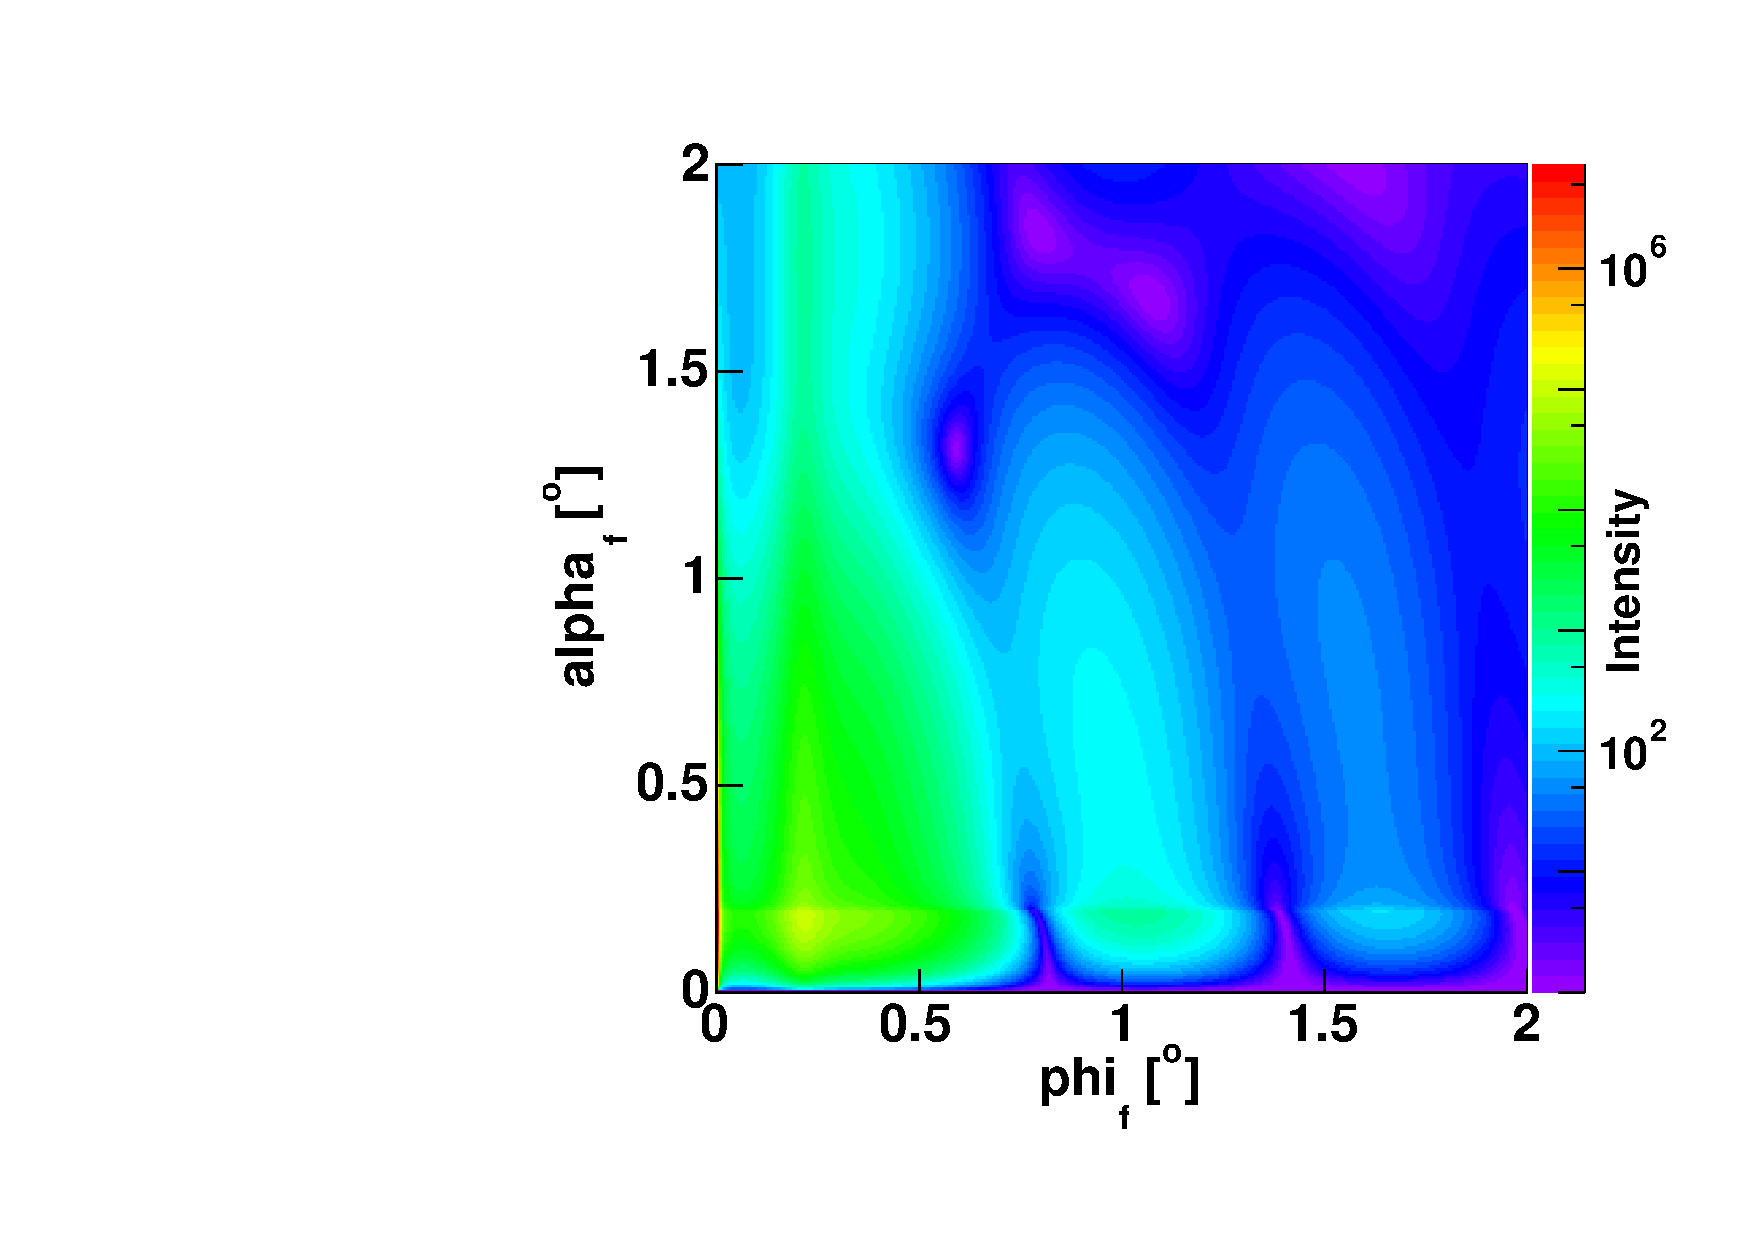
\includegraphics[angle=-90,width=0.5\textwidth]{fig/gisasmap/HSphere_1DDL.pdf}
\end{center}
\caption{Output intensity scattered from a sample made of half-spheres with the radial paracrystal interference between them. This figure has been generated using Script~\ref{lst:1dpara} for the interference function.}
\label{fig:1ddl}
\end{figure}

\FloatBarrier

\newpage
%-------------------------------------------------------------------------------
\subsubsection{\ding{253}  \Code{InterferenceFunction2DLattice(L\_1, L\_2, alpha, xi)}} 
%-------------------------------------------------------------------------------
where ($L_1$, $L_2$, $\alpha$, $\xi$) are shown in figure~\ref{fig:2dlattice} with 
\begin{itemize}
\item[]$L_1$, $L_2$ the lengths of the lattice cell, 
\item[]$\alpha$ the angle between the lattice basis vectors $\mathbf{a}, \mathbf{b}$ in direct space,
\item[] $\xi$ is the angle defining the lattice orientation (set to $0$ by default); it is taken as the angle between the $\mathbf{a}$ vector of the lattice basis and the $\mathbf{x}$ axis of the reference Cartesian frame (as shown in figure~\ref{fig:multil3d}).
\end{itemize}

\begin{figure}[ht]
\begin{center}
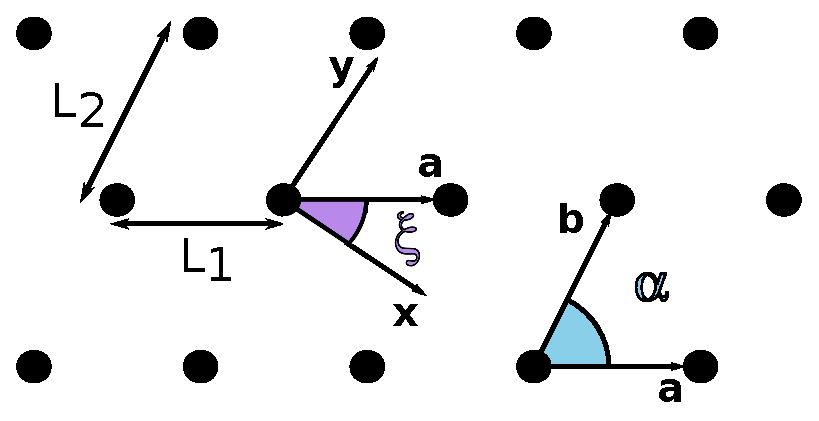
\includegraphics[width=0.5\textwidth]{fig/drawing/2Dlattice.eps}
\end{center}
\caption{Schematic representation of a 2D lattice (top view). Such a lattice is characterized by lattice lengths $L_1$, $L_2$ and angles $\alpha$ and $\xi$.}
\label{fig:2dlattice}
\end{figure}

Like for the one-dimensional case, a probability distribution function \Code{pdf} has to be defined. One can choose between those listed in Section~\ref{baftd} and implements it using \Code{setProbabilityDistribution(pdf)}.

\paragraph{Example} The sample used to run the simulation is made of half-spheres deposited on a substrate. The interference function is "2Dlattice" and the particles are located at the nodes of a square lattice with $L_1=L_2=20$~nm, $\mathbf{a}\equiv \mathbf{b}$ and the probability distribution function is Gaussian. We also use the Decoupling Approximation. 

\begin{lstlisting}[language=python, style=eclipseboxed,numbers=none,nolol,caption={\Code{Python} script to define a 2DLattice interference function between hemi-spherical particles as well as the Decoupling Approximation in \Code{getSimulation()}.  The part specific to the interferences is marked in a red italic font.},label={lst:2dlatticeinterf}]
    #collection of particles
    sphere_ff = FormFactorTruncatedSphere(5*nanometer, 5*nanometer)
    sphere = Particle(m_particle, sphere_ff)
    |interference = InterferenceFunction2DLattice(20.0*nanometer, 20.0*nanometer, 90.0*degree, 0.0*degree)|
    |pdf = FTDistribution2DGauss(200.0*nanometer/2.0/M_PI, 75.0*nanometer/2.0/M_PI)|
    |interference.setProbabilityDistribution(pdf)|
    particle_layout = ParticleLayout()
    particle_layout.addParticle(sphere, 0.0, 1.0)
    |particle_layout.addInterferenceFunction(interference)|

    # interference approx chosen between: DA (default) and SSCA
    |particle_layout.setApproximation(ILayout.DA)|
\end{lstlisting}
 
%\begin{lstlisting}[language=python, style=eclipseboxed,numbers=none,nolol]
%def get_simulation():
%    """
%    Create and return GISAXS simulation with beam and detector
%    """
%    simulation = Simulation()
%    simulation.setDetectorParameters(100, 0.0*degree, 2.0*degree, 100, 0.0*degree, 2.0*degree, True)
%    simulation.setBeamParameters(1.0*angstrom, 0.2*degree, 0.0*degree)
%    return simulation
%\end{lstlisting}


\begin{figure}[ht]
\begin{center}
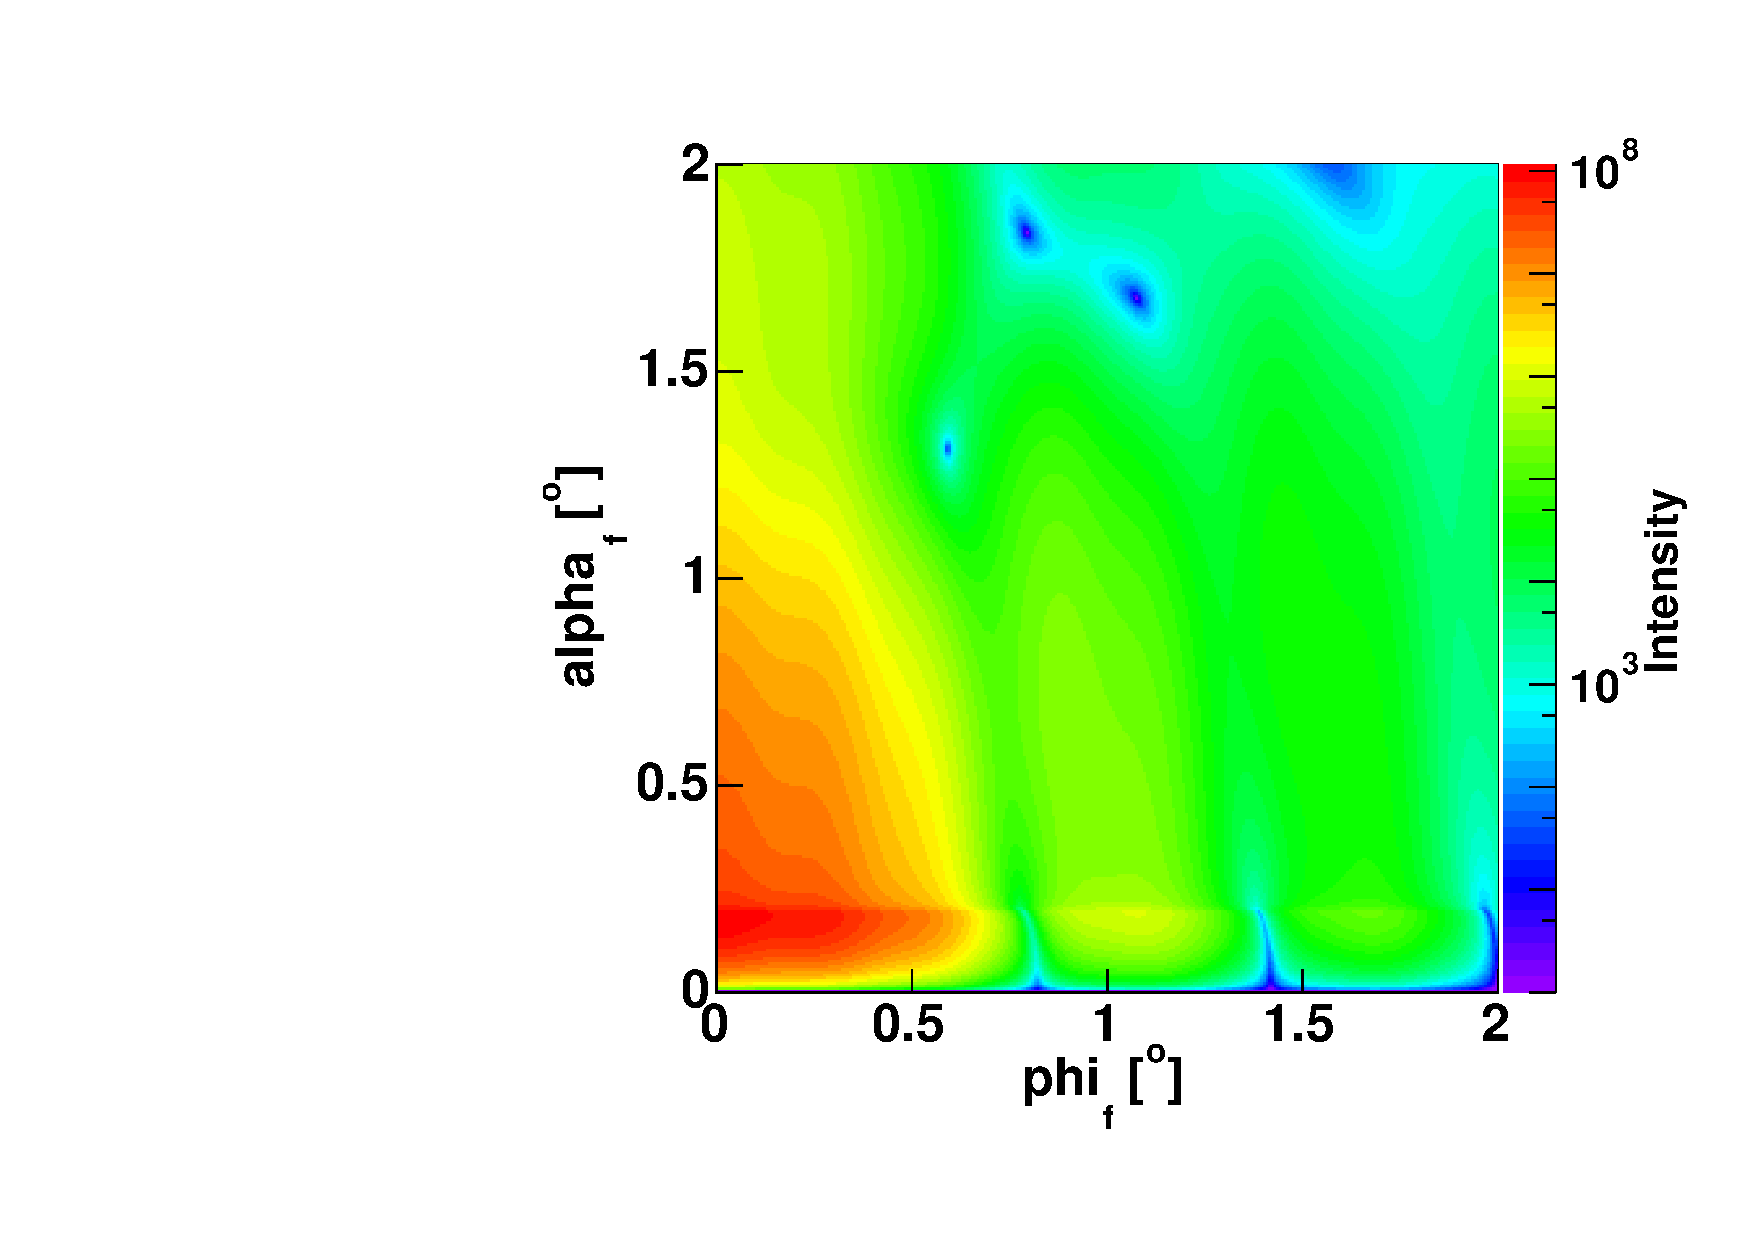
\includegraphics[angle=-90,width=0.5\textwidth]{fig/gisasmap/HSphere_2Dlattice.pdf}
\end{center}
\caption{Output intensity scattered from a sample made of half-spheres with 2DLattice interference function in the Decoupling Approximation.}
\label{fig:2dlatticeintensity}
\end{figure}

\FloatBarrier

\newpage%{\cleardoublepage}
%-------------------------------------------------------------------------------
\subsubsection{\ding{253} \Code{InterferenceFunction2DParaCrystal(L\_1, L\_2, lattice\_angle, $\xi$, damping\_length)}} 
%-------------------------------------------------------------------------------
\begin{itemize}
\item[where] $L_1$, $L_2$ are the lengths of the lattice cell,
\item[] lattice\_angle the angle between the lattice basis vectors $\mathbf{a}, \mathbf{b}$ in direct space,
\item[] $\xi$ is the angle defining the lattice orientation (set to $0$ by default).
\item[] \Code{damping\_length} is used to introduce finite size effects by applying a multiplicative coefficient equal to  $\exp$(-\Code{peak\_distance/damping\_length}) to the Fourier transform of the probability densities. \Code{damping\_length} is equal to 0 by default and, in this case, no correction is applied.
\end{itemize}
Two predefined interference functions can also be used:
\begin{itemize}
\item  \Code{createSquare(peak\_distance, damping\_length, domain\_size\_1, domain\_size\_2)}\\
where the angle between the base vectors of the lattice is set to $\pi/2$,
it creates a squared lattice,
\item \Code{createHexagonal(peak\_distance, damping\_length, domain\_size\_1, domain\_size\_2)}\\
where the angle between the base vectors of the lattice is set to $2\pi/3$ ,
\end{itemize}
where
\Code{domain\_size1, 2} are the dimensions of coherent domains of the paracrystal along the main axes,\\ \Code{peak\_distance} is the same in both directions and $\mathbf{a}\equiv \mathbf{x}$.\\

Probability distribution functions have to be defined. As the two-dimensional paracrystal is defined from two independent one-dimensional paracrystals, we need two of these functions, using\\ \Code{setProbabilityDistributions(pdf\_1, pdf\_2)}, with \Code{pdf\_{1,2}} related to each main axis of the paracrystal (see figure~\ref{fig:2dparaschematic}).


\begin{figure}[ht]
\begin{center}
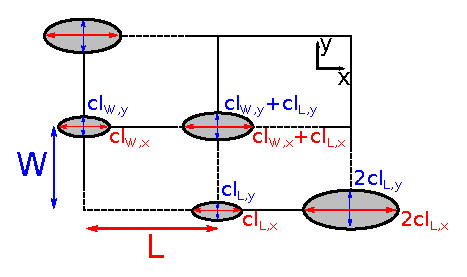
\includegraphics[width=0.75\textwidth]{fig/drawing/drawing2Dparacrystal.eps}
\end{center}
\caption{Schematics of the ideal 2D paracrystal. The gray-shaded areas mark the regions where the probability to find a node is larger that the width at half-maximum of the distribution. $L$ and  $W$ are the mean inter-node distances along the two crystallographic axes. cl$_{(L,W),(x,y)}$ are the widths of the distribution of distance. The disorder is propagated as we add more nodes. Such a structure would be generated using \Code{InterferenceFunction2DParacrystal(L,W,90.*degrees,0,damp\_length)}, with \Code{pdf$_1$ = FTDistribution2DGauss(cl$_{L,x}$,cl$_{L,y}$)} and  \Code{pdf$_2$ = FTDistribution2DGauss(cl$_{W,x}$,cl$_{W,y}$)}.}
\label{fig:2dparaschematic}
\end{figure}


\paragraph{Example} The particles deposited on a substrate are half-spheres. The scattered beams interference via the 2DParacrystal distribution function. The paracrystal is based on a 2D hexagonal lattice with a Gaussian probability distribution function in reciprocal space.  Script~\ref{lst:2dparainterf} shows the implementation of the interference function and fig.~\ref{fig:2ddl} an example of output intensity using hemi-spherical particles.

\begin{lstlisting}[language=python, style=eclipseboxed,numbers=none,nolol,caption={\Code{Python} script to define a "2DParacrystal" interference function between particles forming an hexagonal monolayer. },label={lst:2dparainterf}]
    interference = InterferenceFunction2DParaCrystal.createHexagonal(30.0*nanometer,0.0, 40.0*micrometer, 40.0*micrometer)|
    pdf = FTDistribution2DCauchy(1.0*nanometer, 1.0*nanometer)
    interference.setProbabilityDistributions(pdf, pdf)
    particle_layout.addInterferenceFunction(interference)
\end{lstlisting}

\begin{figure}[ht]
\begin{center}
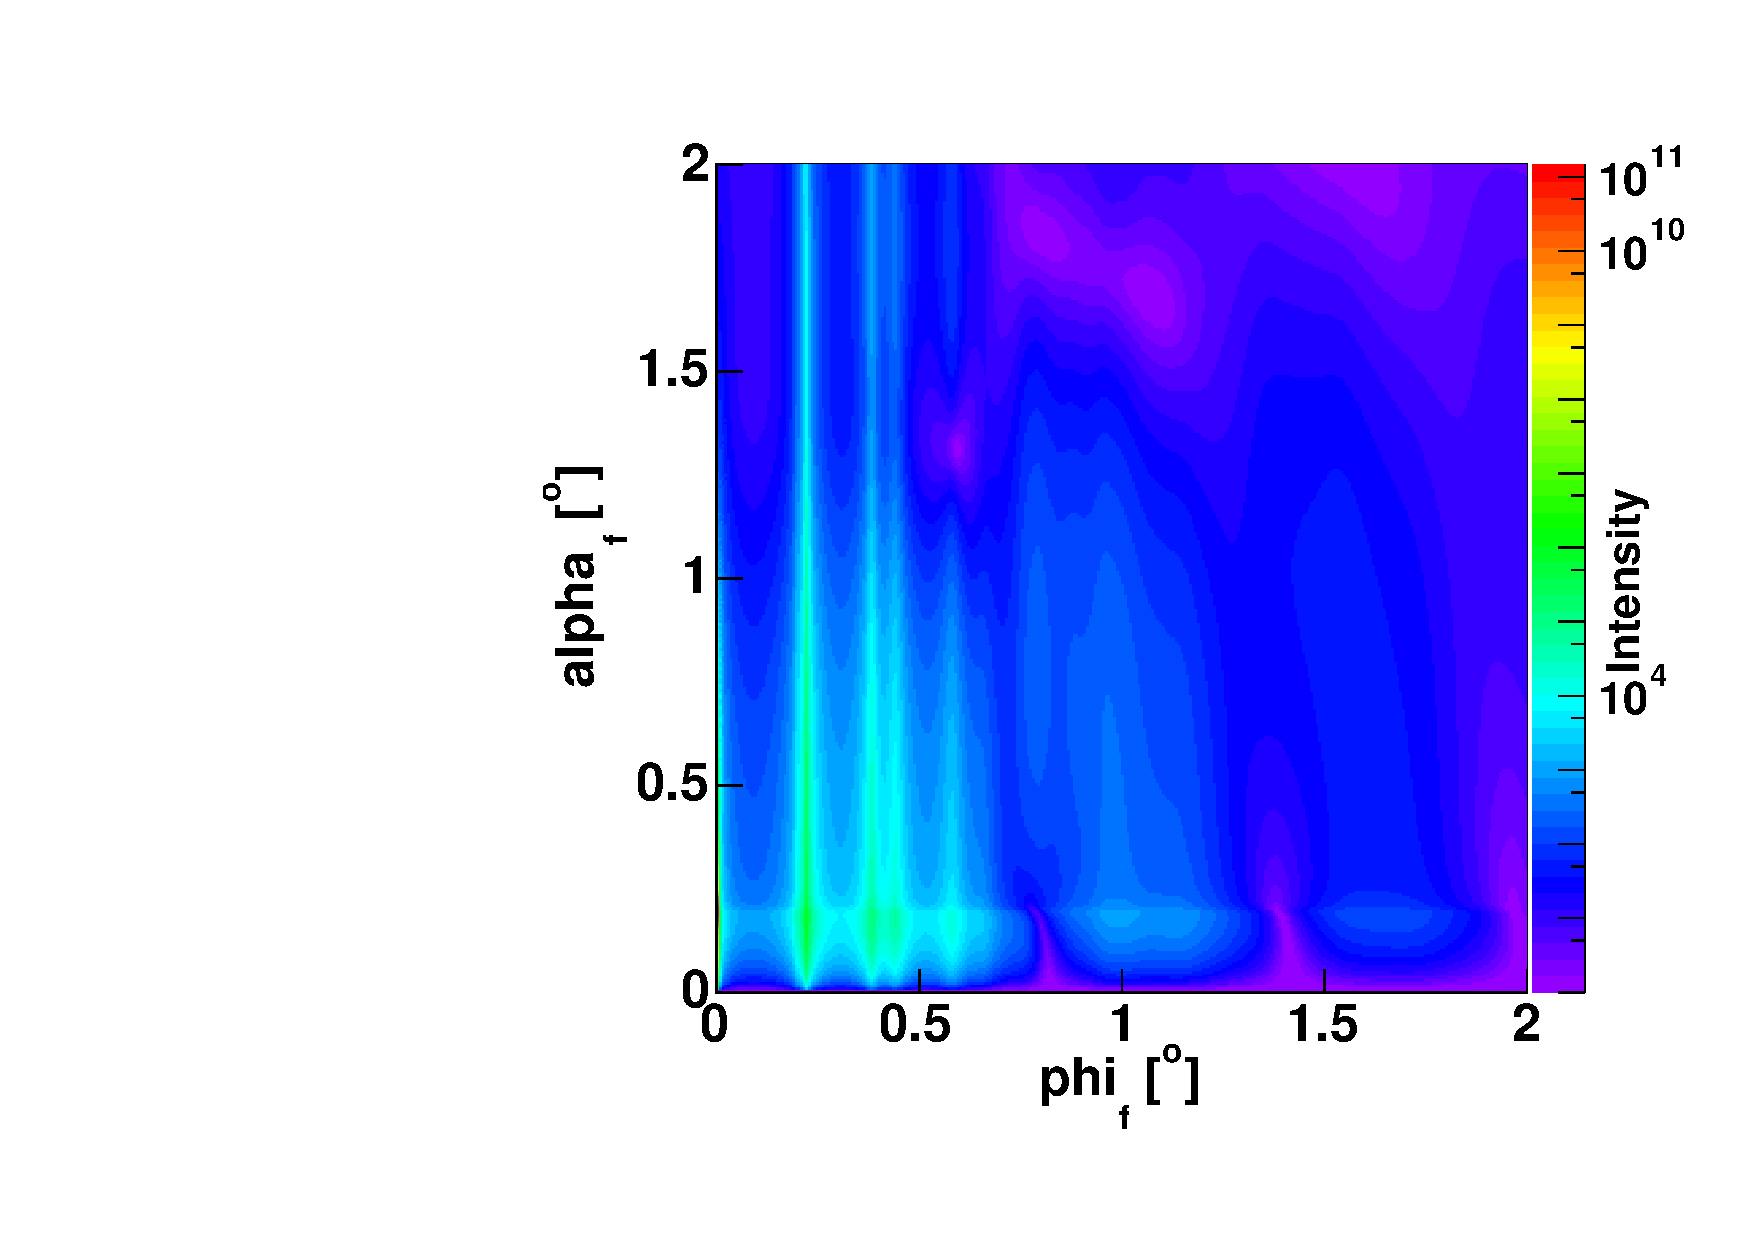
\includegraphics[angle=-90,width=0.5\textwidth]{fig/gisasmap/HSphere_2DDL.pdf}
\end{center}
\caption{Output intensity scattered from a sample made of half-spheres with 2DParacrystal interference function.}
\label{fig:2ddl}
\end{figure}

\FloatBarrier


%===============================================================================
\subsection{Summary}
%===============================================================================

\begin{table}[h]
\begin{tabular}{lll}
\hline
Name & Characteristics &  Comments \\
\hline
DA & no correlations& implemented with \Code{setApproximation} \\
     & & default option \\
\hline
LMA & sample = groups of particles & automatic implementation if several \\ 
 & of identical sizes and shapes & \Code{ParticleLayout}s are defined \\
\hline
SSCA & distance between particles =  &  - implemented with \Code{setApproximation} \\
 &function of their sizes&  - dimensionless coupling coefficient $\kappa$ is \\
 & & required using \Code{setKappa}.\\
\hline
\hline
\end{tabular}
\caption{List of size-distribution models implemented in \BornAgain.}
\end{table}

\FloatBarrier

\begin{landscape}
\begin{table}
\begin{tabular}{lll}
\hline
Function  & Parameters & Comments\\
\hline
\Code{InterferenceFunctionNone}  & None & disordered distribution \\
\hline
\Code{InterferenceFunction1DLattice} & \Code{lattice\_length} & use only with infinitely long/wide particles \\
  & $\xi=\widehat{(\mathbf{x},\mathbf{a})}$ & pdf=(Cauchy, Gauss or Voigt)  to be defined\\
\hline
 \Code{InterferenceFunctionRadialParaCrystal}  & peak\_distance of pdf & pdf=(Cauchy, Gauss or Voigt) to be defined \\
& damping\_length (optional) & \\
\hline
 \Code{InterferenceFunction2DLattice}  & L\_1, L\_2: lattice lengths & pdf=(Cauchy, Gauss or Voigt) to be defined\\
                        & lattice\_angle=$\widehat{(\mathbf{a},\mathbf{b})}$ & \\
                                                            & $\xi =\widehat{(\mathbf{x},\mathbf{a})}$ & \\                                                  
\hline
\Code{InterferenceFunction2DParaCrystal}  & L\_1, L\_2: lattice lengths & 2D pdf=(Cauchy, Gauss or Voigt) to be defined \\
                          & lattice\_angle=$\widehat{(\mathbf{a},\mathbf{b})}$ & (1 pdf per axis) \\
& $\xi=\widehat{(\mathbf{x},\mathbf{a})}$ & \\
& damping\_length (optional)  &  same for both axes\\
\hline
\hline
\end{tabular}
\caption{List of interference functions implemented in \BornAgain. pdf : probability distribution function, $\mathbf{a}, \mathbf{b}$ are the lattice base vectors, and $\mathbf{x}$ is the axis vector perpendicular to the detector plane.}
\end{table}
\end{landscape}


%%%%%%%%%%%%%%%%%%%%%%%%%%%%%%%%%%%%%%%%%%%%%%%%%%%%%%%%%%%%%%%%%%%%%%%%%%%%%%%%
\section{Particle shapes}
%%%%%%%%%%%%%%%%%%%%%%%%%%%%%%%%%%%%%%%%%%%%%%%%%%%%%%%%%%%%%%%%%%%%%%%%%%%%%%%%

\index{Form factors|(}
\index{Shape transform}
The form factor of a hard-shell particle is its \textit{shape transform}
\begin{equation}
F(\mathbf{q})=\int_V \exp (i\mathbf{q}.\mathbf{r}) d^3 \mathbf{r},
\label{ffformulaBA}
\end{equation}
where $V$ is the volume of the particle,
$\mathbf{q}=\mathbf{k}_i - \mathbf{k}_f$ is the scattering vector with
$\mathbf{k}_f$ and $\mathbf{k}_i$ the scattered and incident wave
vector, respectively.\\

The particle's shape is parametrized in a Cartesian frame, with its
$z$-axis pointing upwards and its origin at the center of the bottom
of the particle: $\mathbf{r}=(x,y,z)$. 

All form factors have been implemented with complex scattering vectors
in order to take any material absorption into account.

In \BornAgain\ the expression of the form factor has been implemented in the Born approximation. Each of them is defined as
\begin{equation*}
F(\mathbf{q})=\int_V \exp (i\mathbf{q}.\mathbf{r}) d^3 \mathbf{r},
\end{equation*}
where $V$ is the volume of the particle's shape,
$\mathbf{q}=\mathbf{k}_i - \mathbf{k}_f$ is the scattering vector with
$\mathbf{k}_f$ and $\mathbf{k}_i$ the scattered and incident wave
vector, respectively. The Distorted Wave Born Approximation can be taken into account as it has been explained in \SecRef{sect:dwba}.\\

The particle's shape is parametrized in a Cartesian frame, with its
$z$-axis pointing upwards and its origin at the center of the bottom
of the particle: $\mathbf{r}=(x,y,z)$. In the followings, a schematic view will depict this layout for each
form factor.\\

All form factors have been implemented with complex scattering vectors
in order to take any material absorption into account.\\

%===============================================================================
\subsection{Implemented form factors}
%===============================================================================

Table~\ref{tab:formfactors} lists the shapes whose form
factors have been implemented in \BornAgain.
The following pages document each implemented form factor in detail.


\begin{table}[H] 
\caption{Table of form factors implemented in \BornAgain.} \label{tab:formfactors}
  \begin{tabulary} {\textwidth}{Lc Lc L c L} 
\hline 
Box,\phantom{-} \SecRef{Box} & & Prism3,  \SecRef{Prism3} & & Tetrahedron, \SecRef{Tetrahedron} & & Prism6,  \SecRef{Prism6}\\
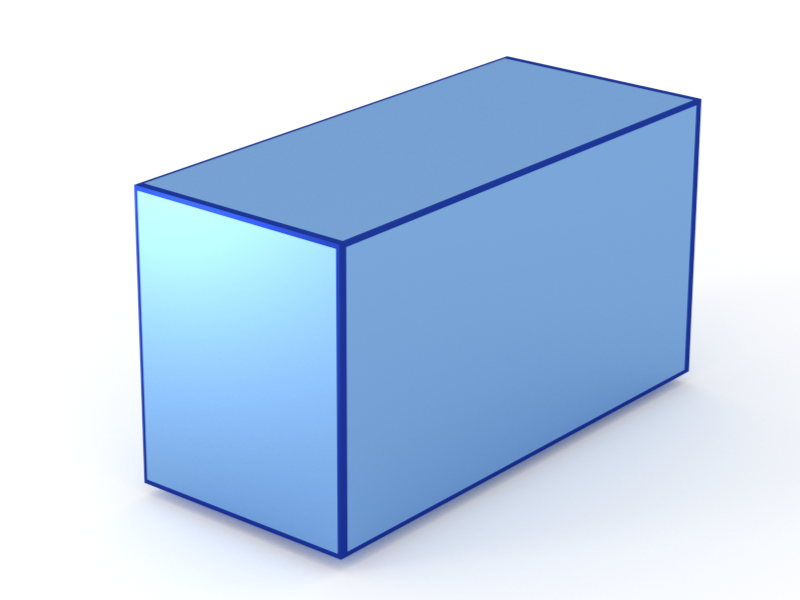
\includegraphics[width=1in]{fig/blue/Box3d.png} & & 
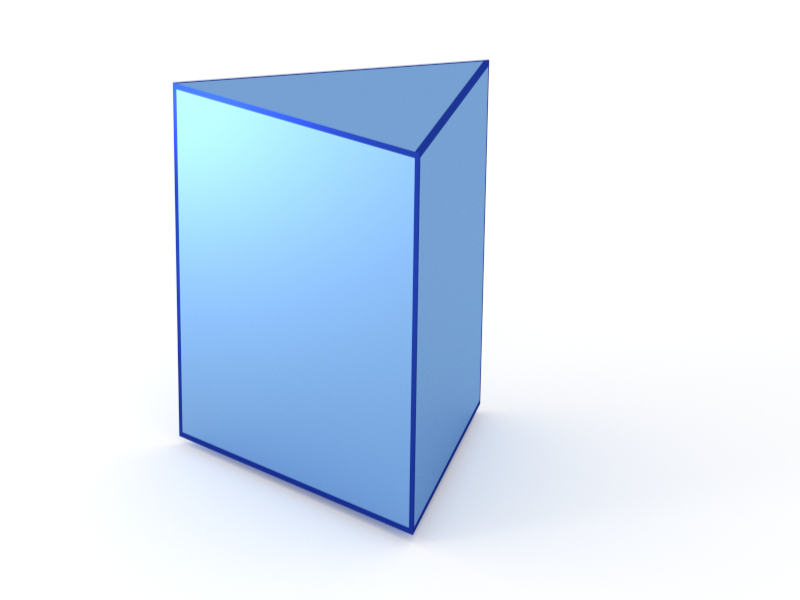
\includegraphics[width=1in]{fig/blue/Prism33d.png} & & 
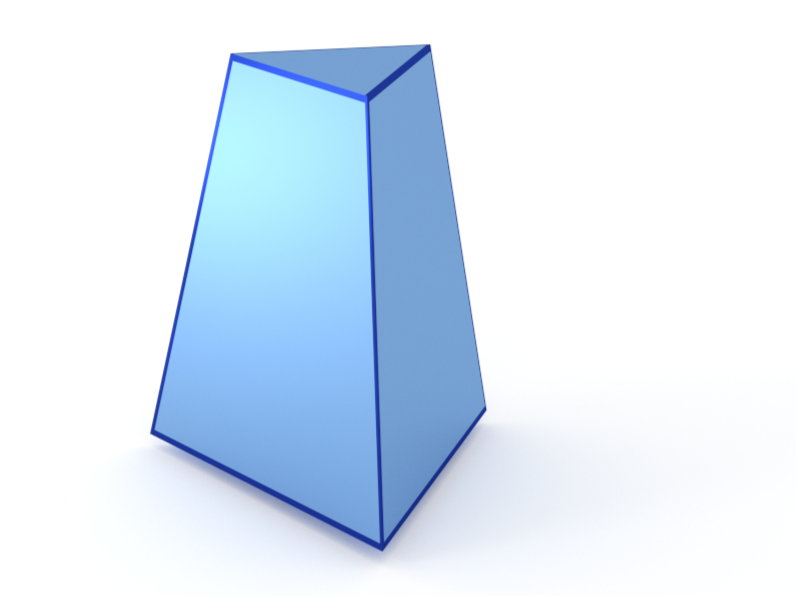
\includegraphics[width=1in]{fig/blue/Tetrahedron3d.png} & & 
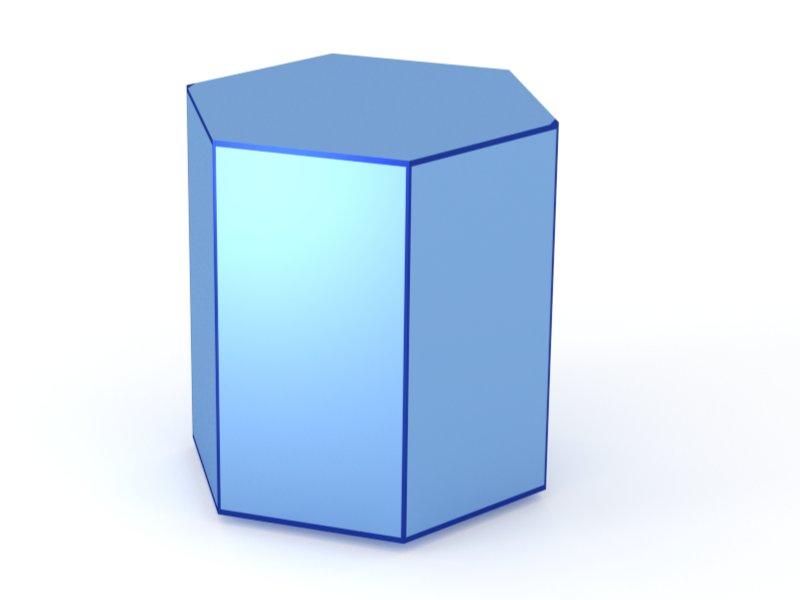
\includegraphics[width=1in]{fig/blue/Prism63d.png} 
\\
\hline 
Cone6,  \SecRef{Cone6} & &  Pyramid, \SecRef{Pyramid} & & Anisotropic pyramid,  \SecRef{AnisoPyramid} & &  {Cuboctahedron}, \SecRef{Cuboctahedron}\\
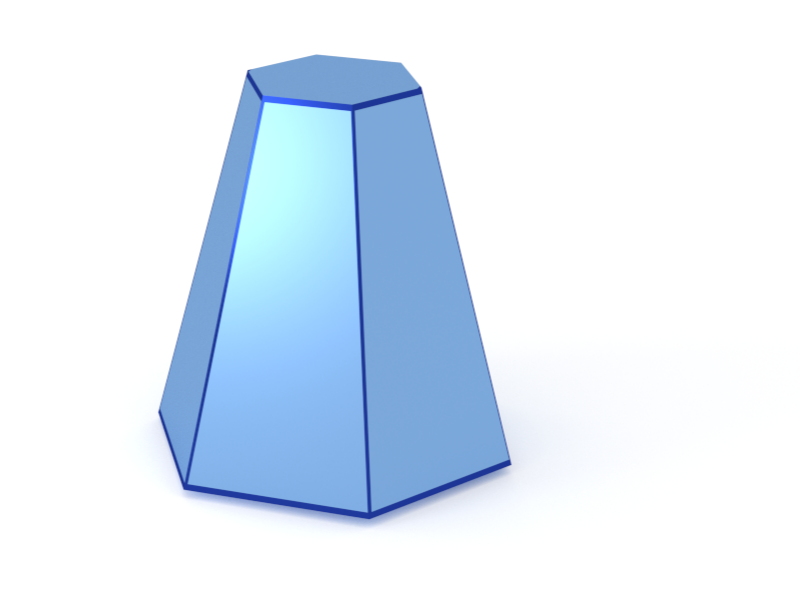
\includegraphics[width=1in]{fig/blue/Cone63d.png}  & & 
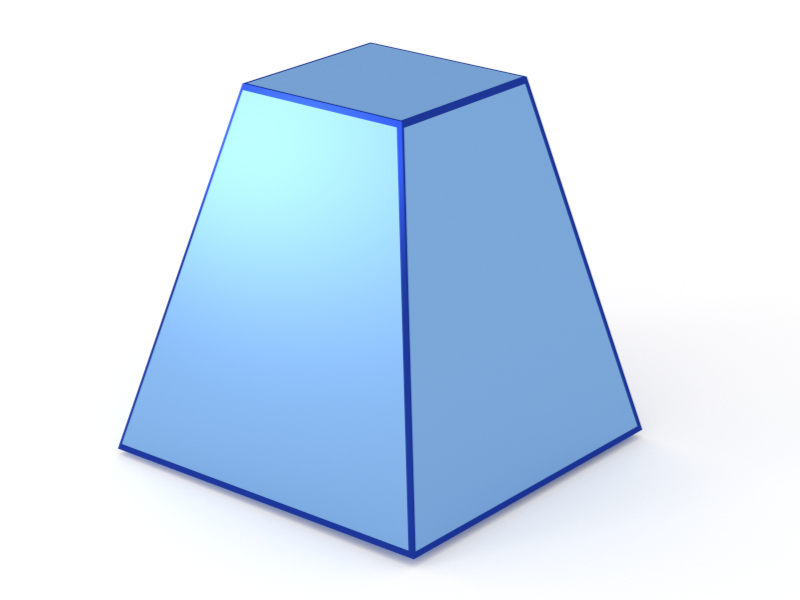
\includegraphics[width=1in]{fig/blue/Pyramid3d.png} & &
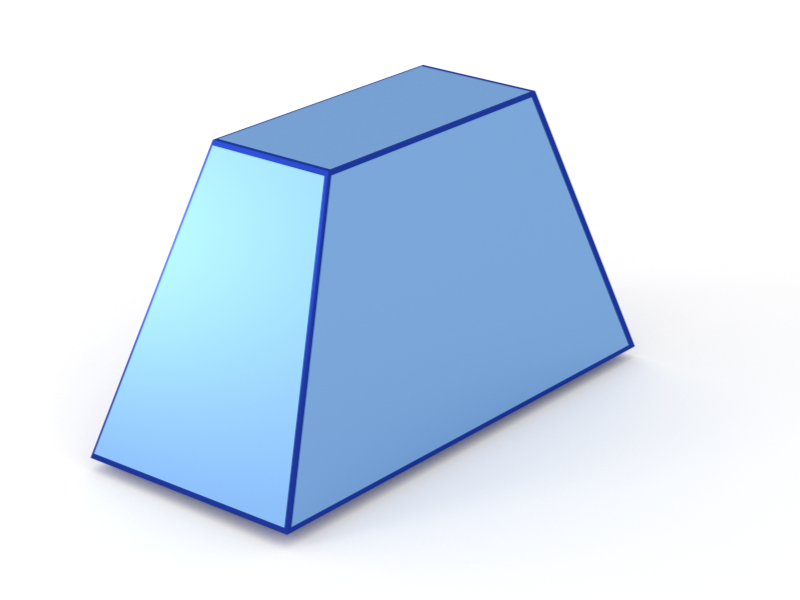
\includegraphics[width=1in]{fig/blue/AnistropicPyramid3d.png} & & 
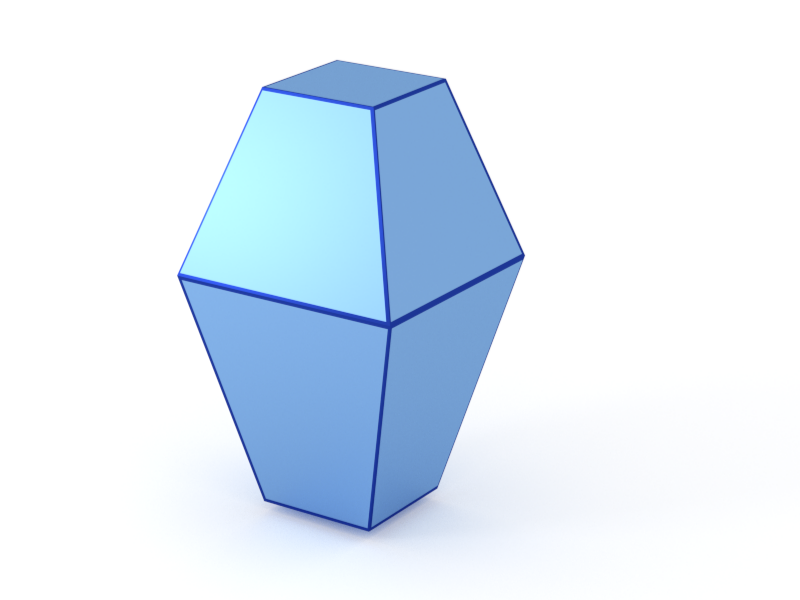
\includegraphics[width=1in]{fig/blue/Cuboctahedron3d.png}
\\
\hline
Cylinder, \SecRef{Cylinder}  & & Ellipsoidal cylinder, \SecRef{EllipsoidalCylinder} & &  Cone,\phantom{--} \SecRef{Cone} & & Full Sphere, \SecRef{FullSphere} \\
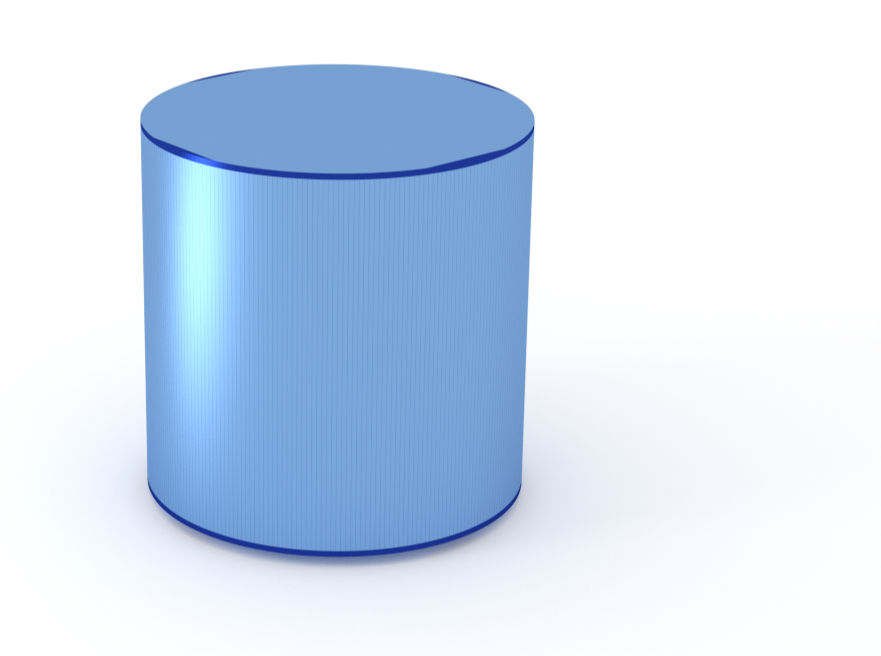
\includegraphics[width=1in]{fig/blue/Cylinder3d.png} & & 
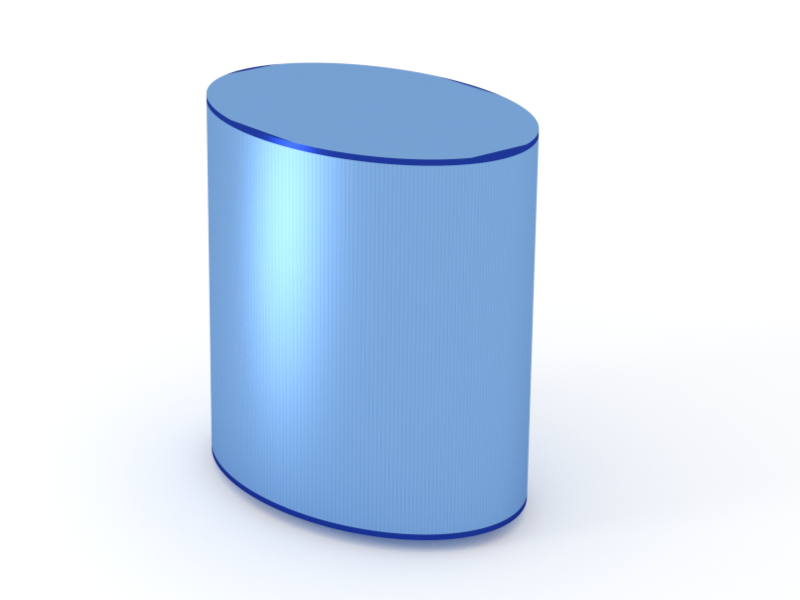
\includegraphics[width=1in]{fig/blue/EllipsoidalCylinder3d.png} & & 
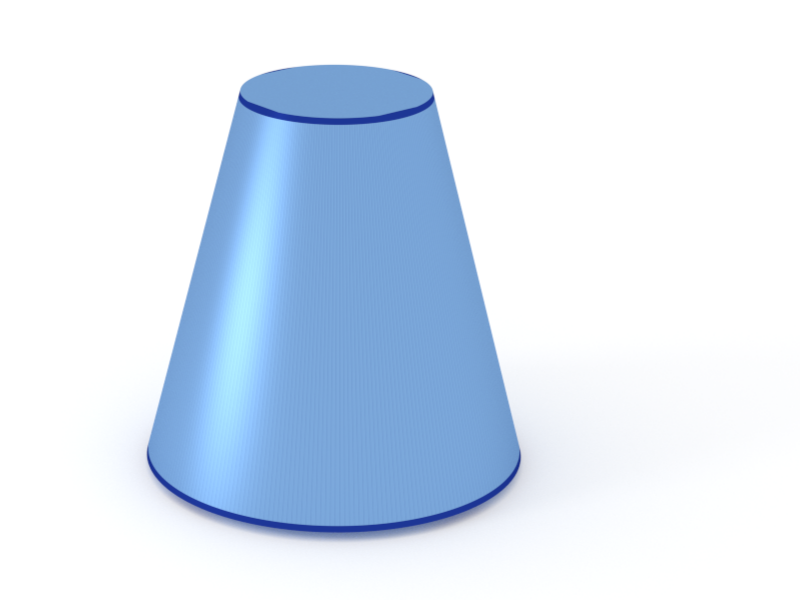
\includegraphics[width=1in]{fig/blue/Cone3d.png} & & 
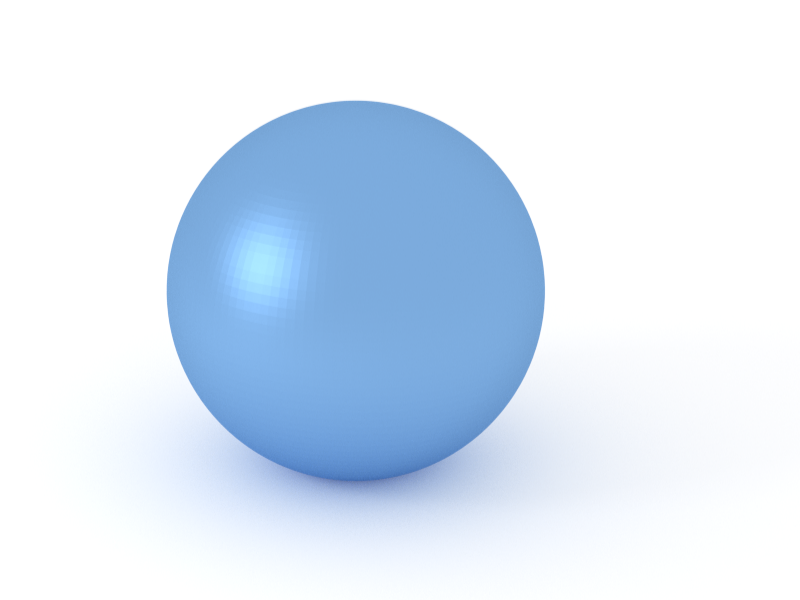
\includegraphics[width=1in]{fig/blue/FullSphere3d.png} \\
\hline
Truncated Sphere, \SecRef{Sphere}  & & Full Spheroid, \SecRef{FullSpheroid} & & Truncated Spheroid,  \SecRef{Spheroid} & & Hemi Ellipsoid, \SecRef{HemiEllipsoid}\\
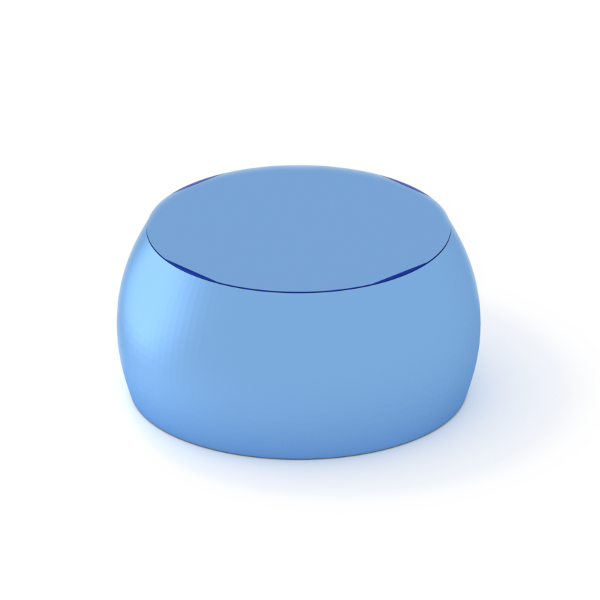
\includegraphics[width=1in]{fig/blue/Sphere3d.png}  & & 
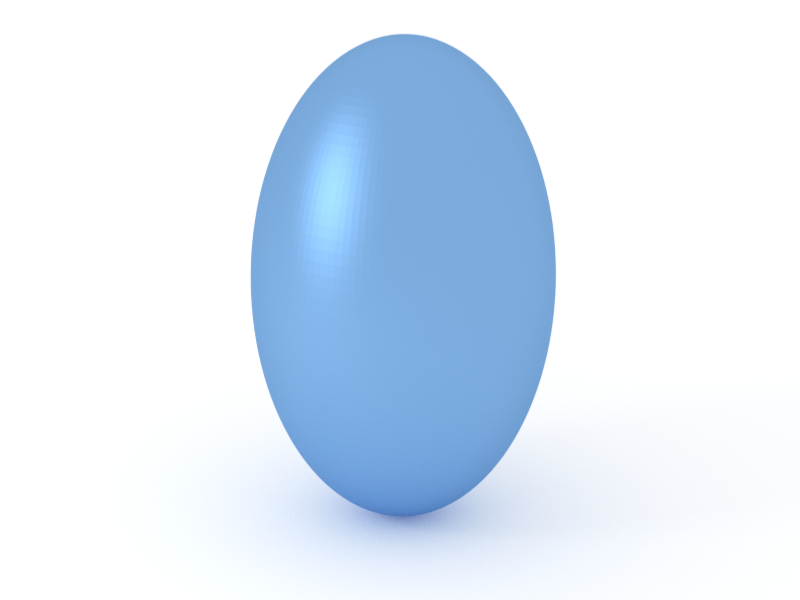
\includegraphics[width=1in]{fig/blue/FullSpheroid3d.png} & & 
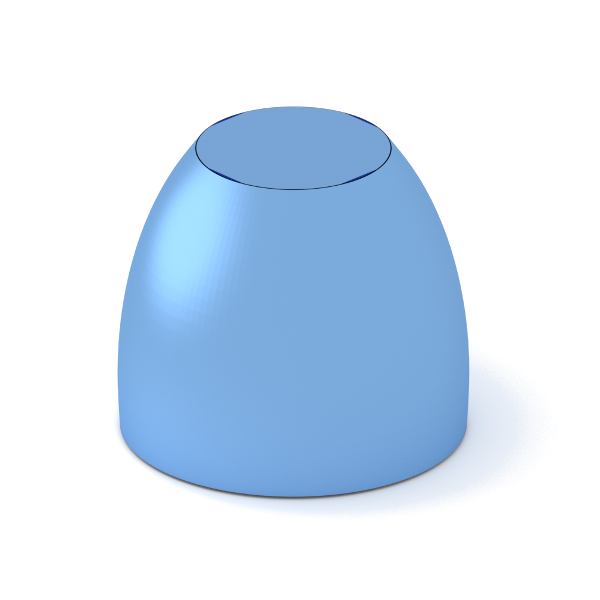
\includegraphics[width=1in]{fig/blue/Spheroid3d.png} & & 
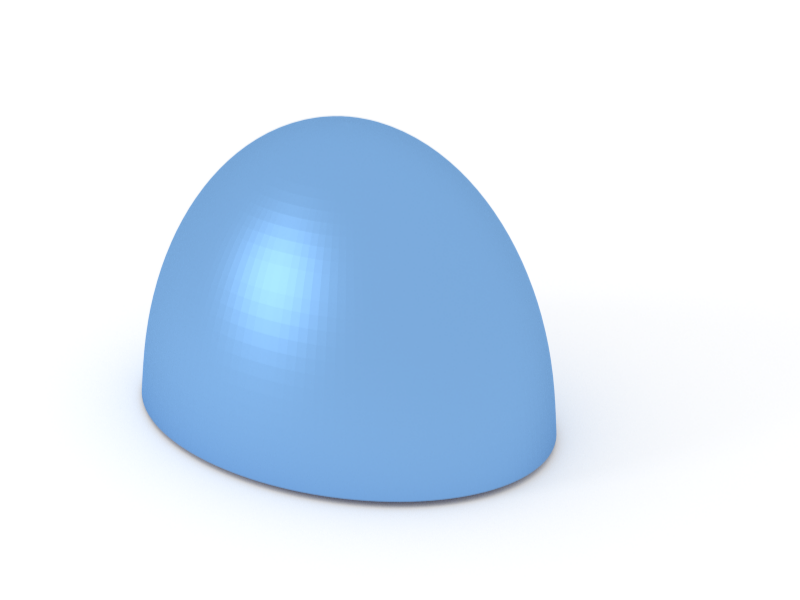
\includegraphics[width=1in]{fig/blue/HemiEllipsoid3d.png}\\
\hline
Ripple1, \SecRef{Ripple1} &  & Ripple2, \SecRef{Ripple2}& &   & &  \\
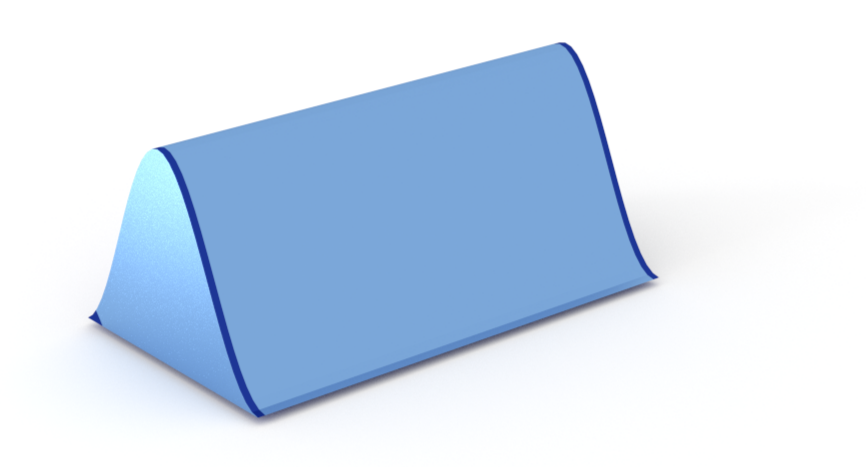
\includegraphics[width=1in]{fig/blue/Ripple13d.png} & & 
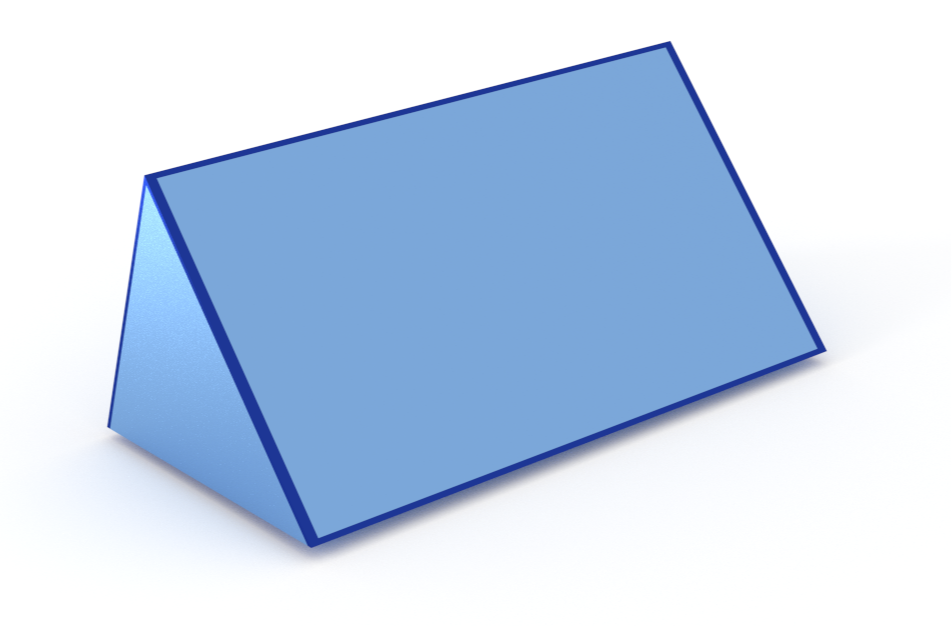
\includegraphics[width=1in]{fig/blue/Ripple23d.png} & &  & & \\
\hline 
\end{tabulary}
\index{Form factors!table of implemented}
\end{table}


%-------------------------------------------------------------------------------
\newpage
\subsubsection{Box (cuboid)} \SecLabel{Box}
  \index{Box (form factor)}
  \index{Cuboid (form factor)}
  \index{Prism (form factor)!reactangular (Box)}
  \index{FormFactorBox@\Code{FormFactorBox}}
%-------------------------------------------------------------------------------

\paragraph{Real-space geometry}\mbox{}\\
This shape is a rectangular cuboid as
shown in fig.~\ref{fig:box}. 

\begin{figure}[ht]
\hfill
\subfigure[Side view]{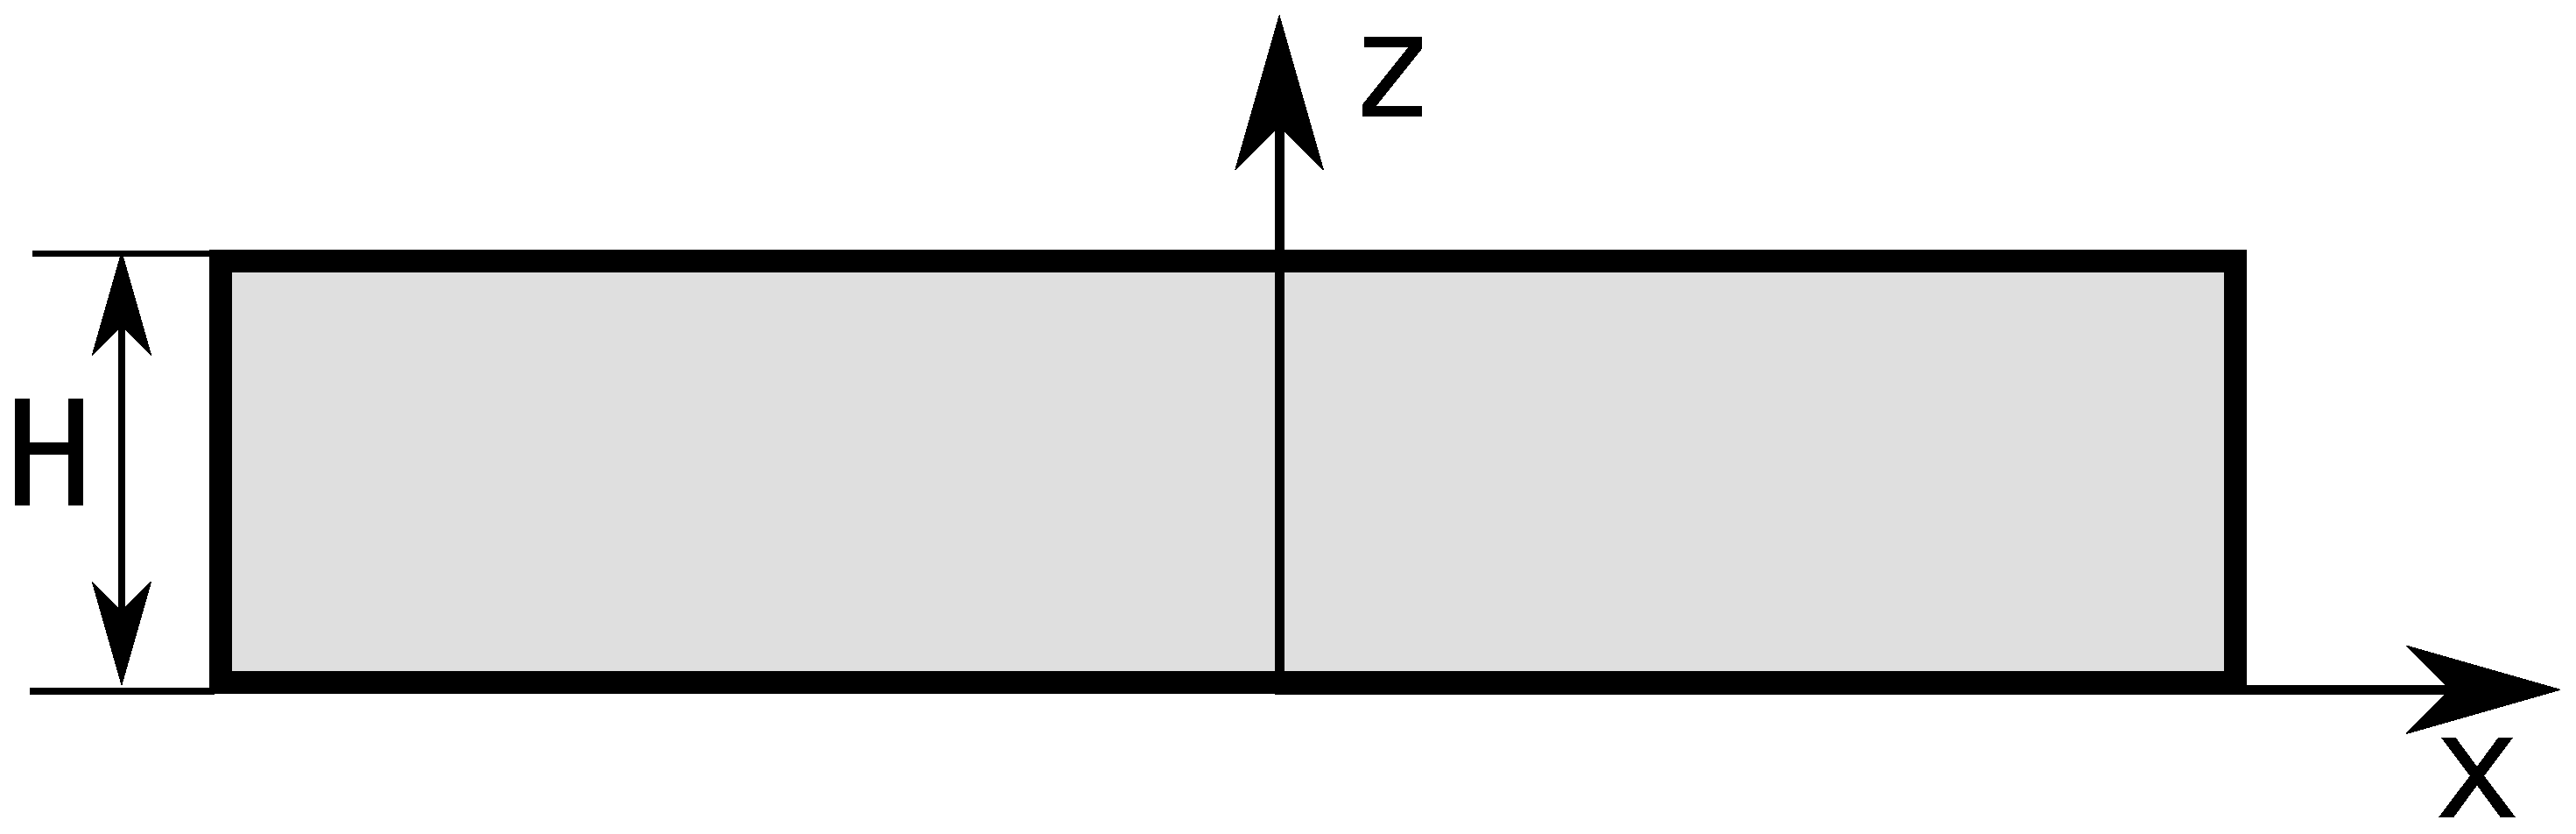
\includegraphics[width=5cm]{fig/cuts/Box2dxz.eps}}
\hfill
\subfigure[Top view]{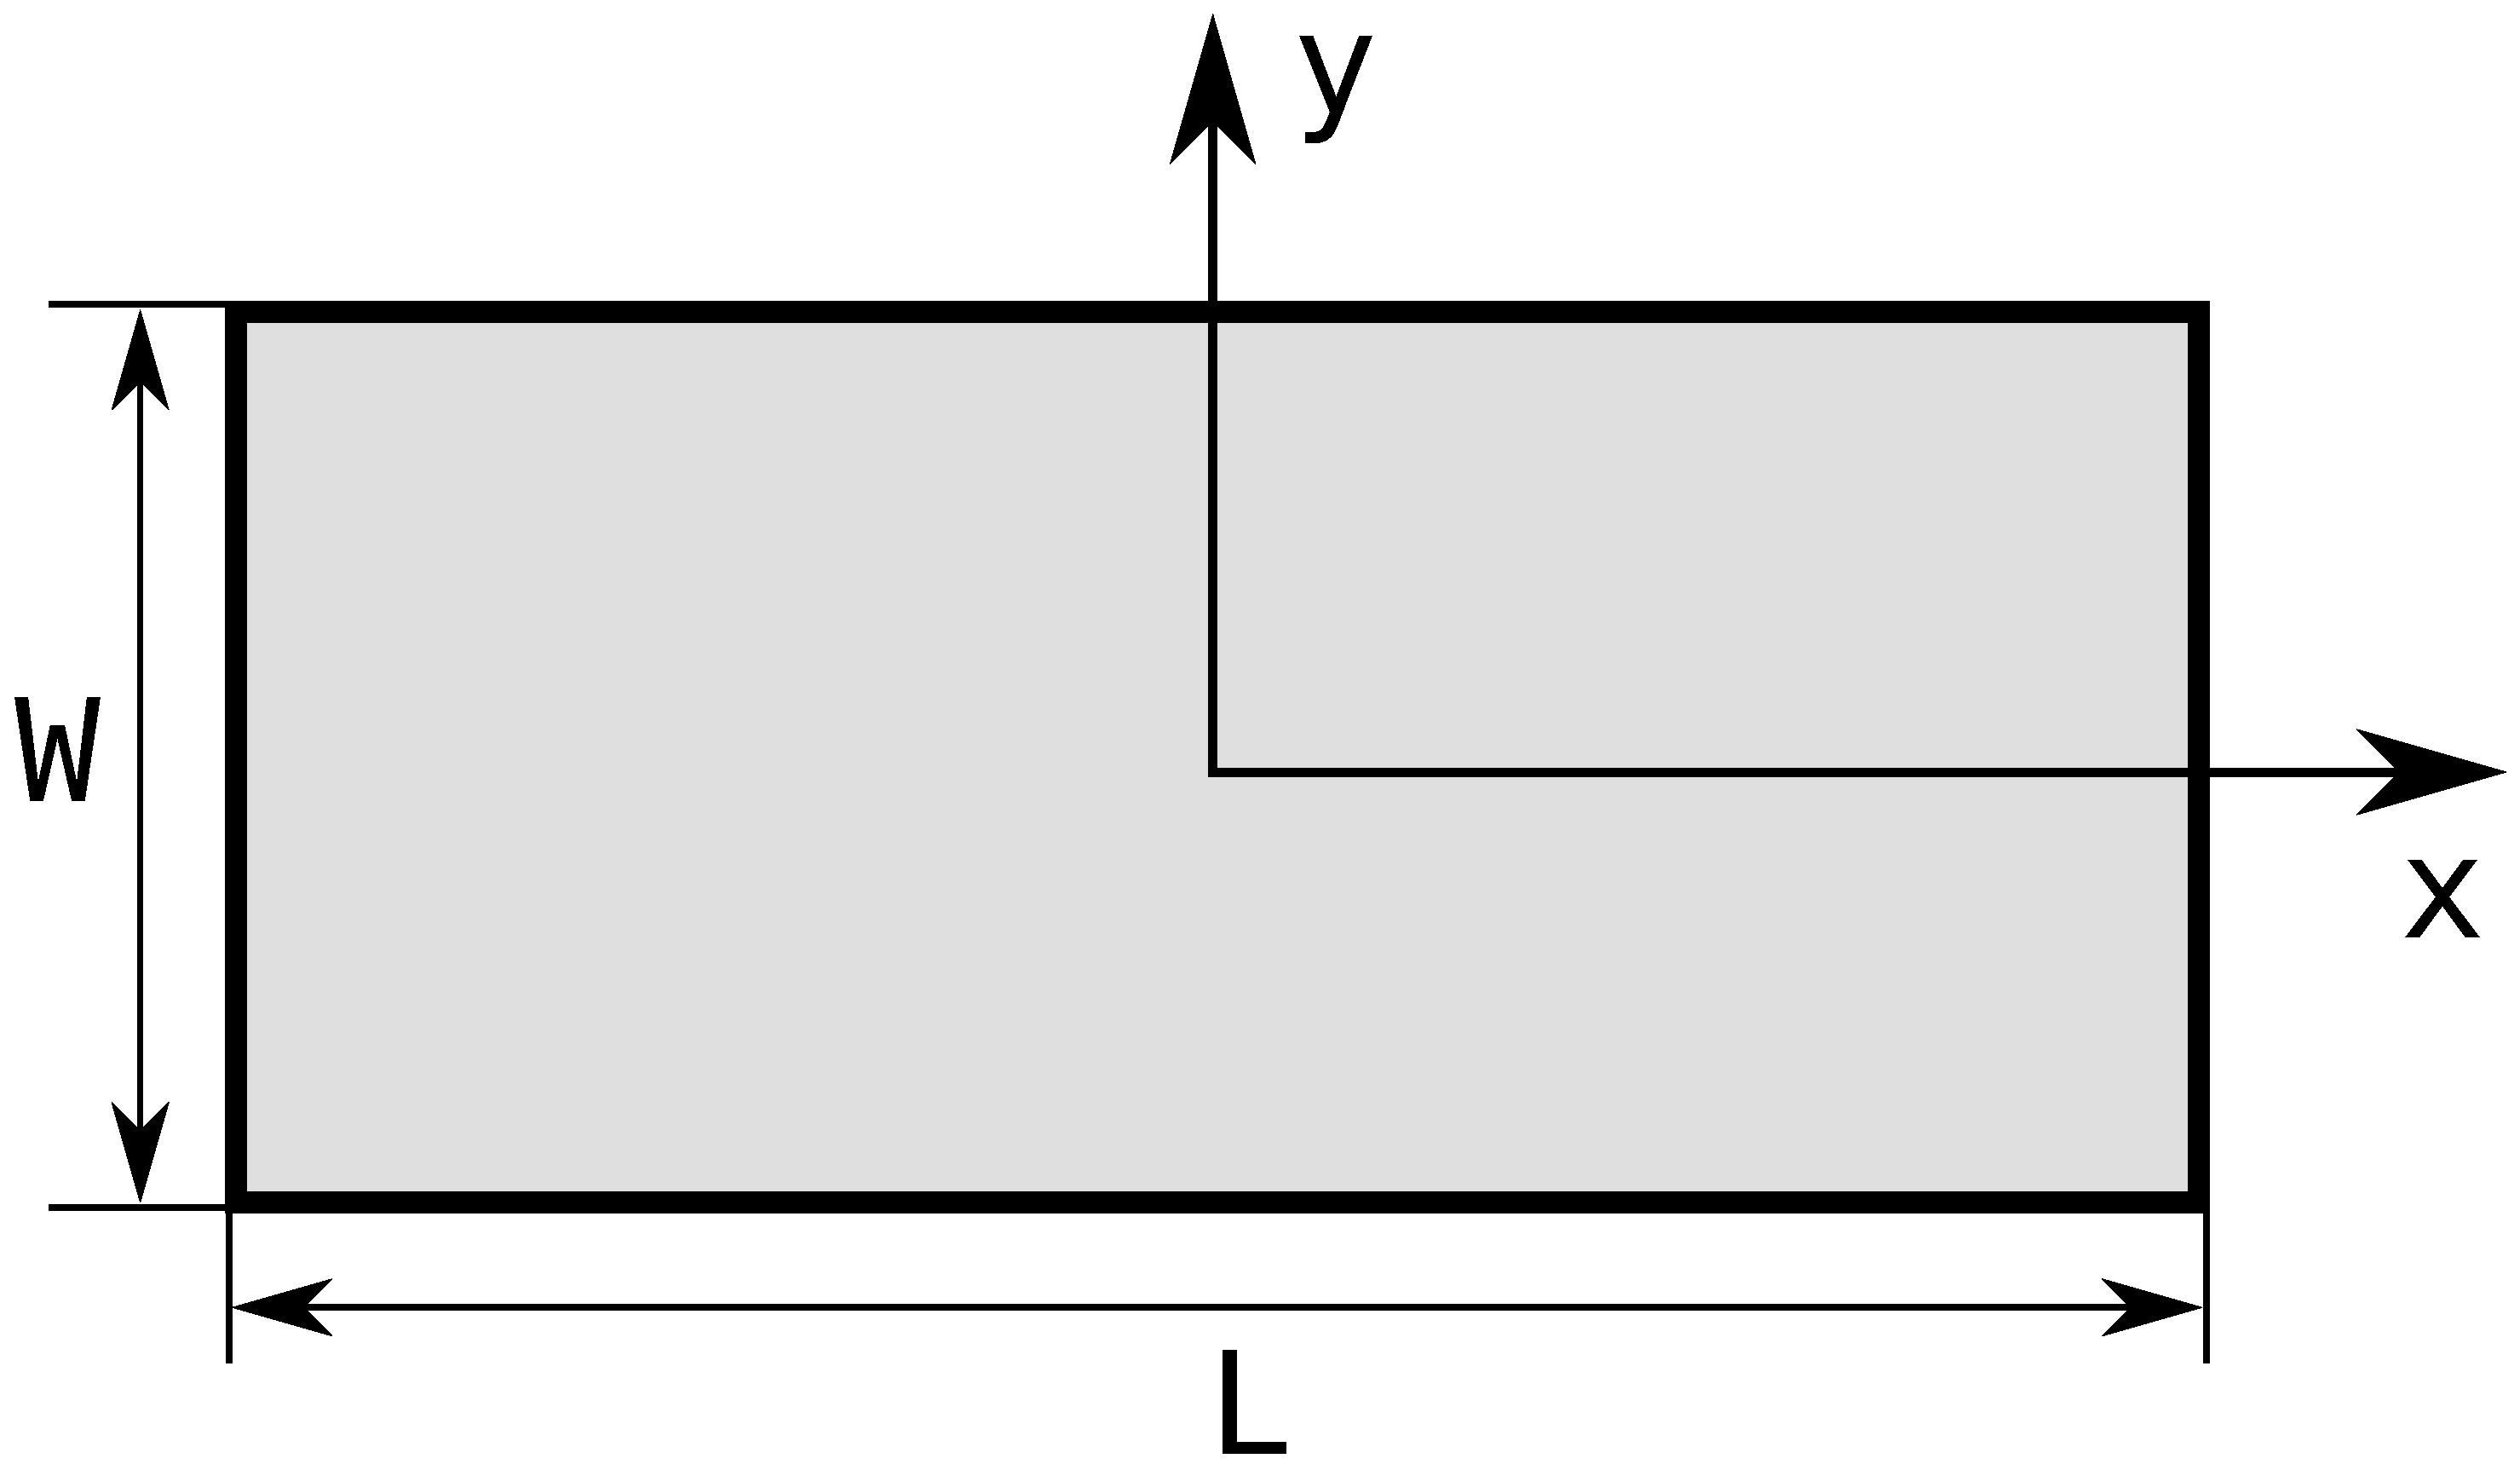
\includegraphics[width=5cm]{fig/cuts/Box2dxy.eps}}
\hfill
\caption{Sketch of a Box.}
\label{fig:box}
\end{figure}

\FloatBarrier

\paragraph{Parameters}
\begin{itemize}
\item length of the base $L$,
\item width of the base $W$,
\item height  $H$.
\end{itemize}

\paragraph{Properties}
\begin{itemize}
\item volume $V= LWH$,
\item particle surface seen from above $S = LW$.
%\item radius of gyration
\end{itemize}

\paragraph{Expression of the form factor}
\begin{equation*}
F(\mathbf{q},L,W,H)= L W H\exp\left(i q_z \frac{H}{2}\right) \sinc\left(q_x \frac{L}{2}\right)
\sinc\left(q_y \frac{W}{2}\right) \sinc\left(q_z \frac{H}{2}\right),
\end{equation*}
   
where $\sinc(x)=\sin(x)/x$ is the cardinal sine.

\paragraph{Syntax} \Code{FormFactorBox(length, width, height)}

\newpage

\paragraph{Example}\mbox{}\\
Figure~\ref{fig:FFBoxEx} shows the normalized intensity
$|F|^2/V^2$, computed with $L=20$~nm, $W=16$~nm, and $H=13$~nm:

\begin{figure}[ht]
\begin{center}
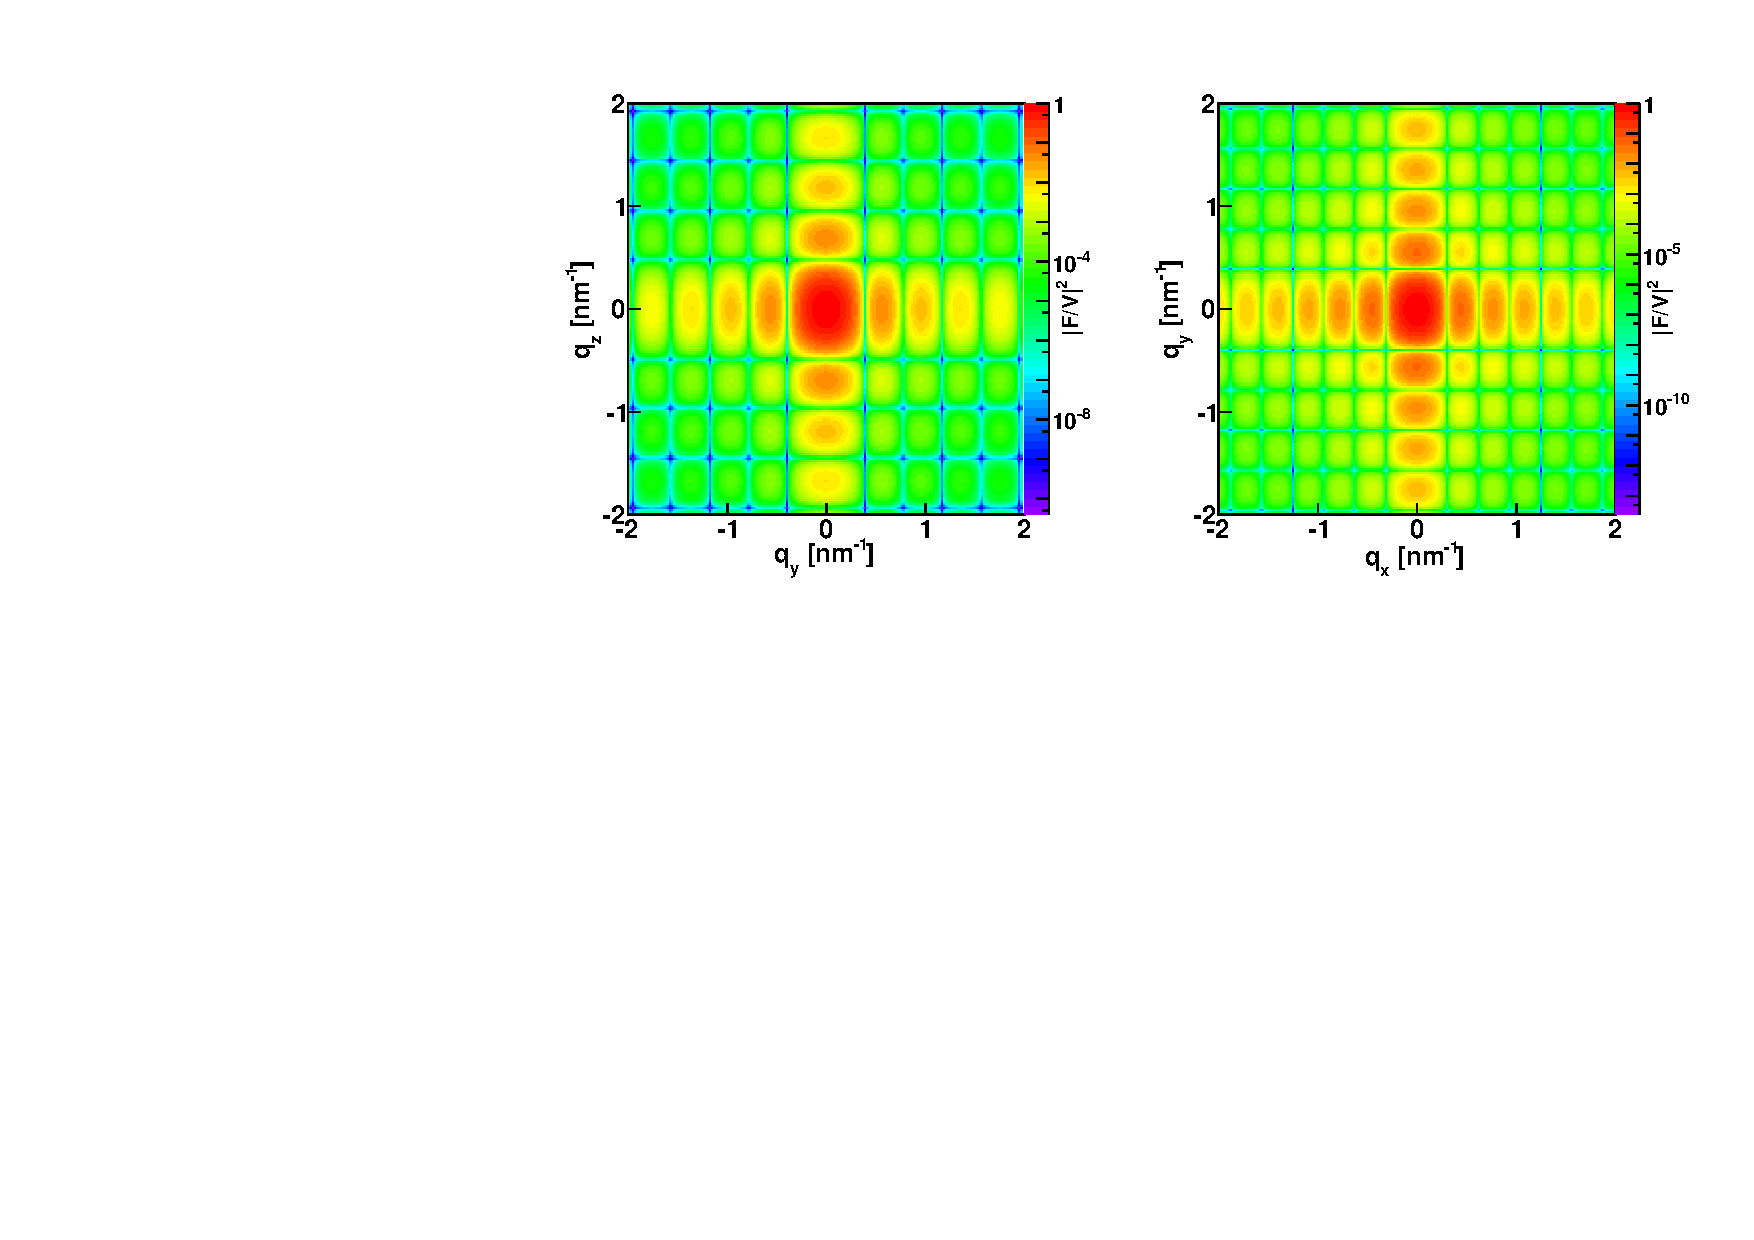
\includegraphics[angle=-90,width=\textwidth]{fig/ff/figffbox.pdf}
\end{center}
\caption{Normalized intensity for the form factor of a Box plotted against ($q_y$, $q_z$) and  ($q_x$, $q_y$) and computed with \Code{FormFactorBox(20.*nanometer, 16.*nanometer, 13.*nanometer)}.}
\label{fig:FFBoxEx}
\end{figure}

\paragraph{References}
Agrees with \lq\lq Box\rq\rq ~form factor of \IsGISAXS~\cite{Laz02},
except for factors $1/2$ in the definitions of parameters $L$, $W$, $H$.

%-------------------------------------------------------------------------------
\newpage
\subsubsection{Prism3 (triangular)} \SecLabel{Prism3}
  \index{Prism (form factor)!triangular (Prism3)}
  \index{FormFactorPrism3@\Code{FormFactorPrism3}}
%-------------------------------------------------------------------------------

\paragraph{Real-space geometry}\mbox{}\\
This shape is a triangular prism, whose base is an equilateral
triangle as shown in fig.~\ref{fig:prism3}.

\begin{figure}[ht]
\hfill
\subfigure[Side view]{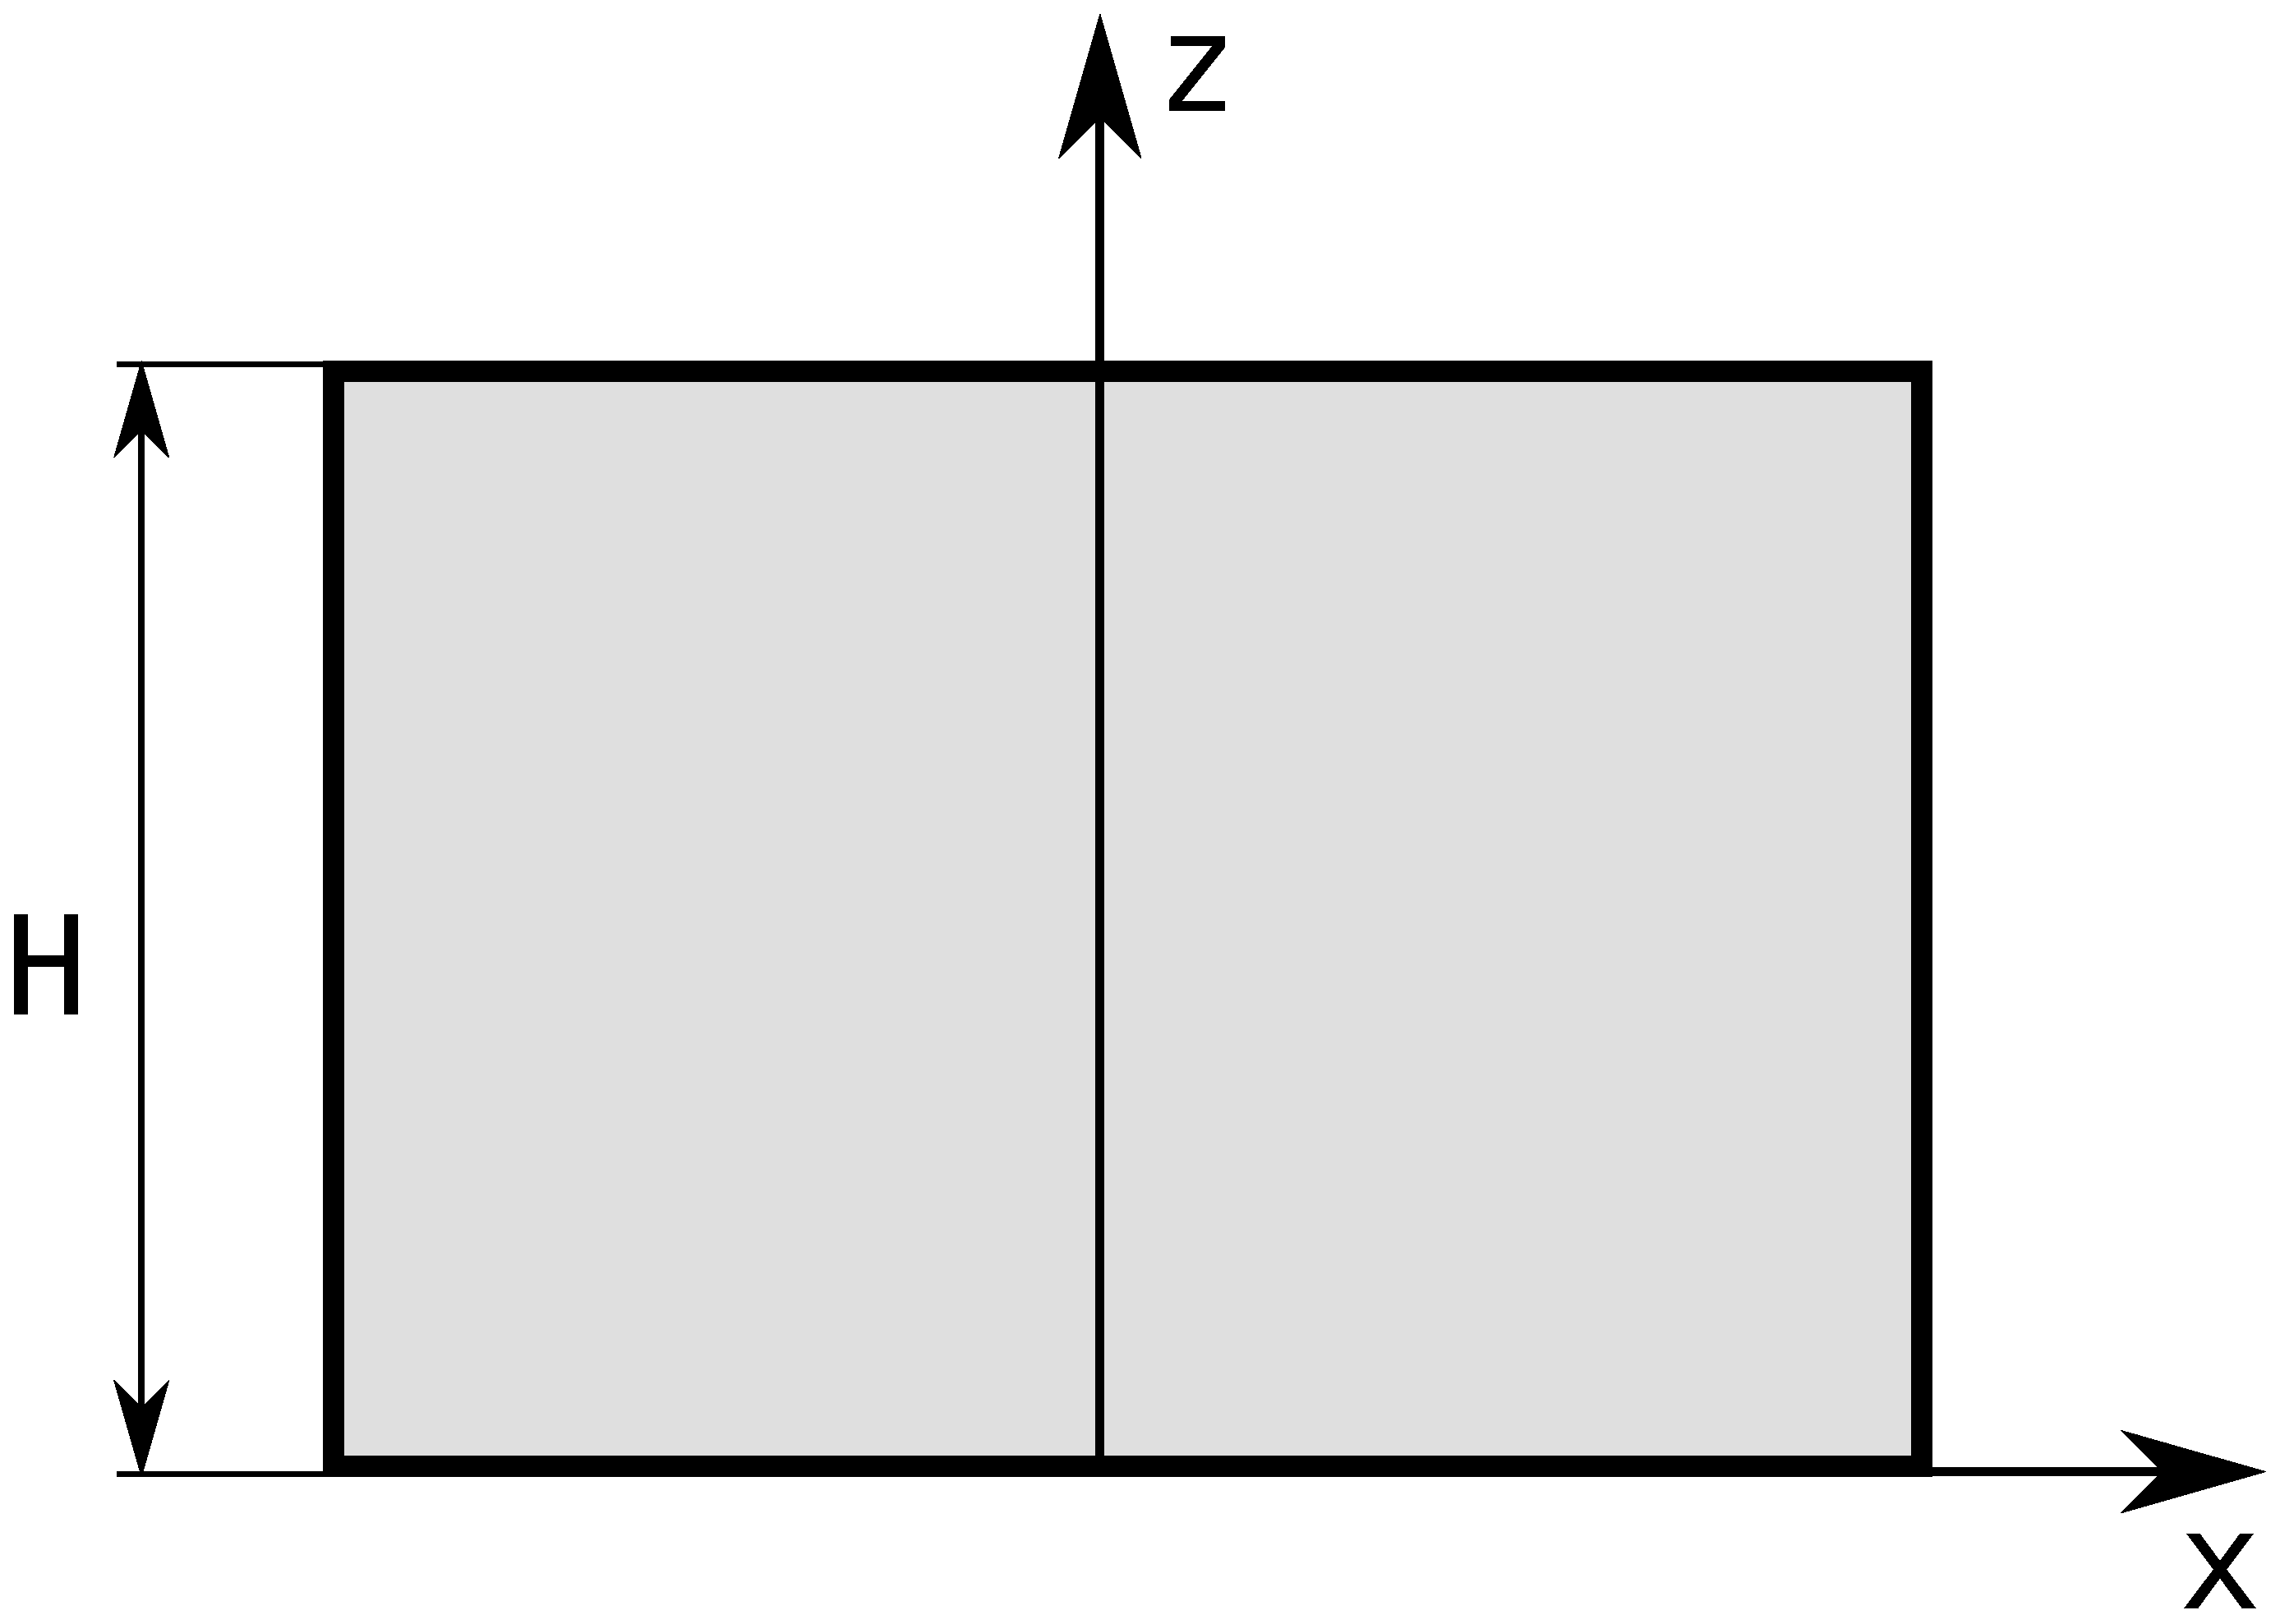
\includegraphics[width=5cm]{fig/cuts/Prism32dxz.eps}}
\hfill
\subfigure[Top view]{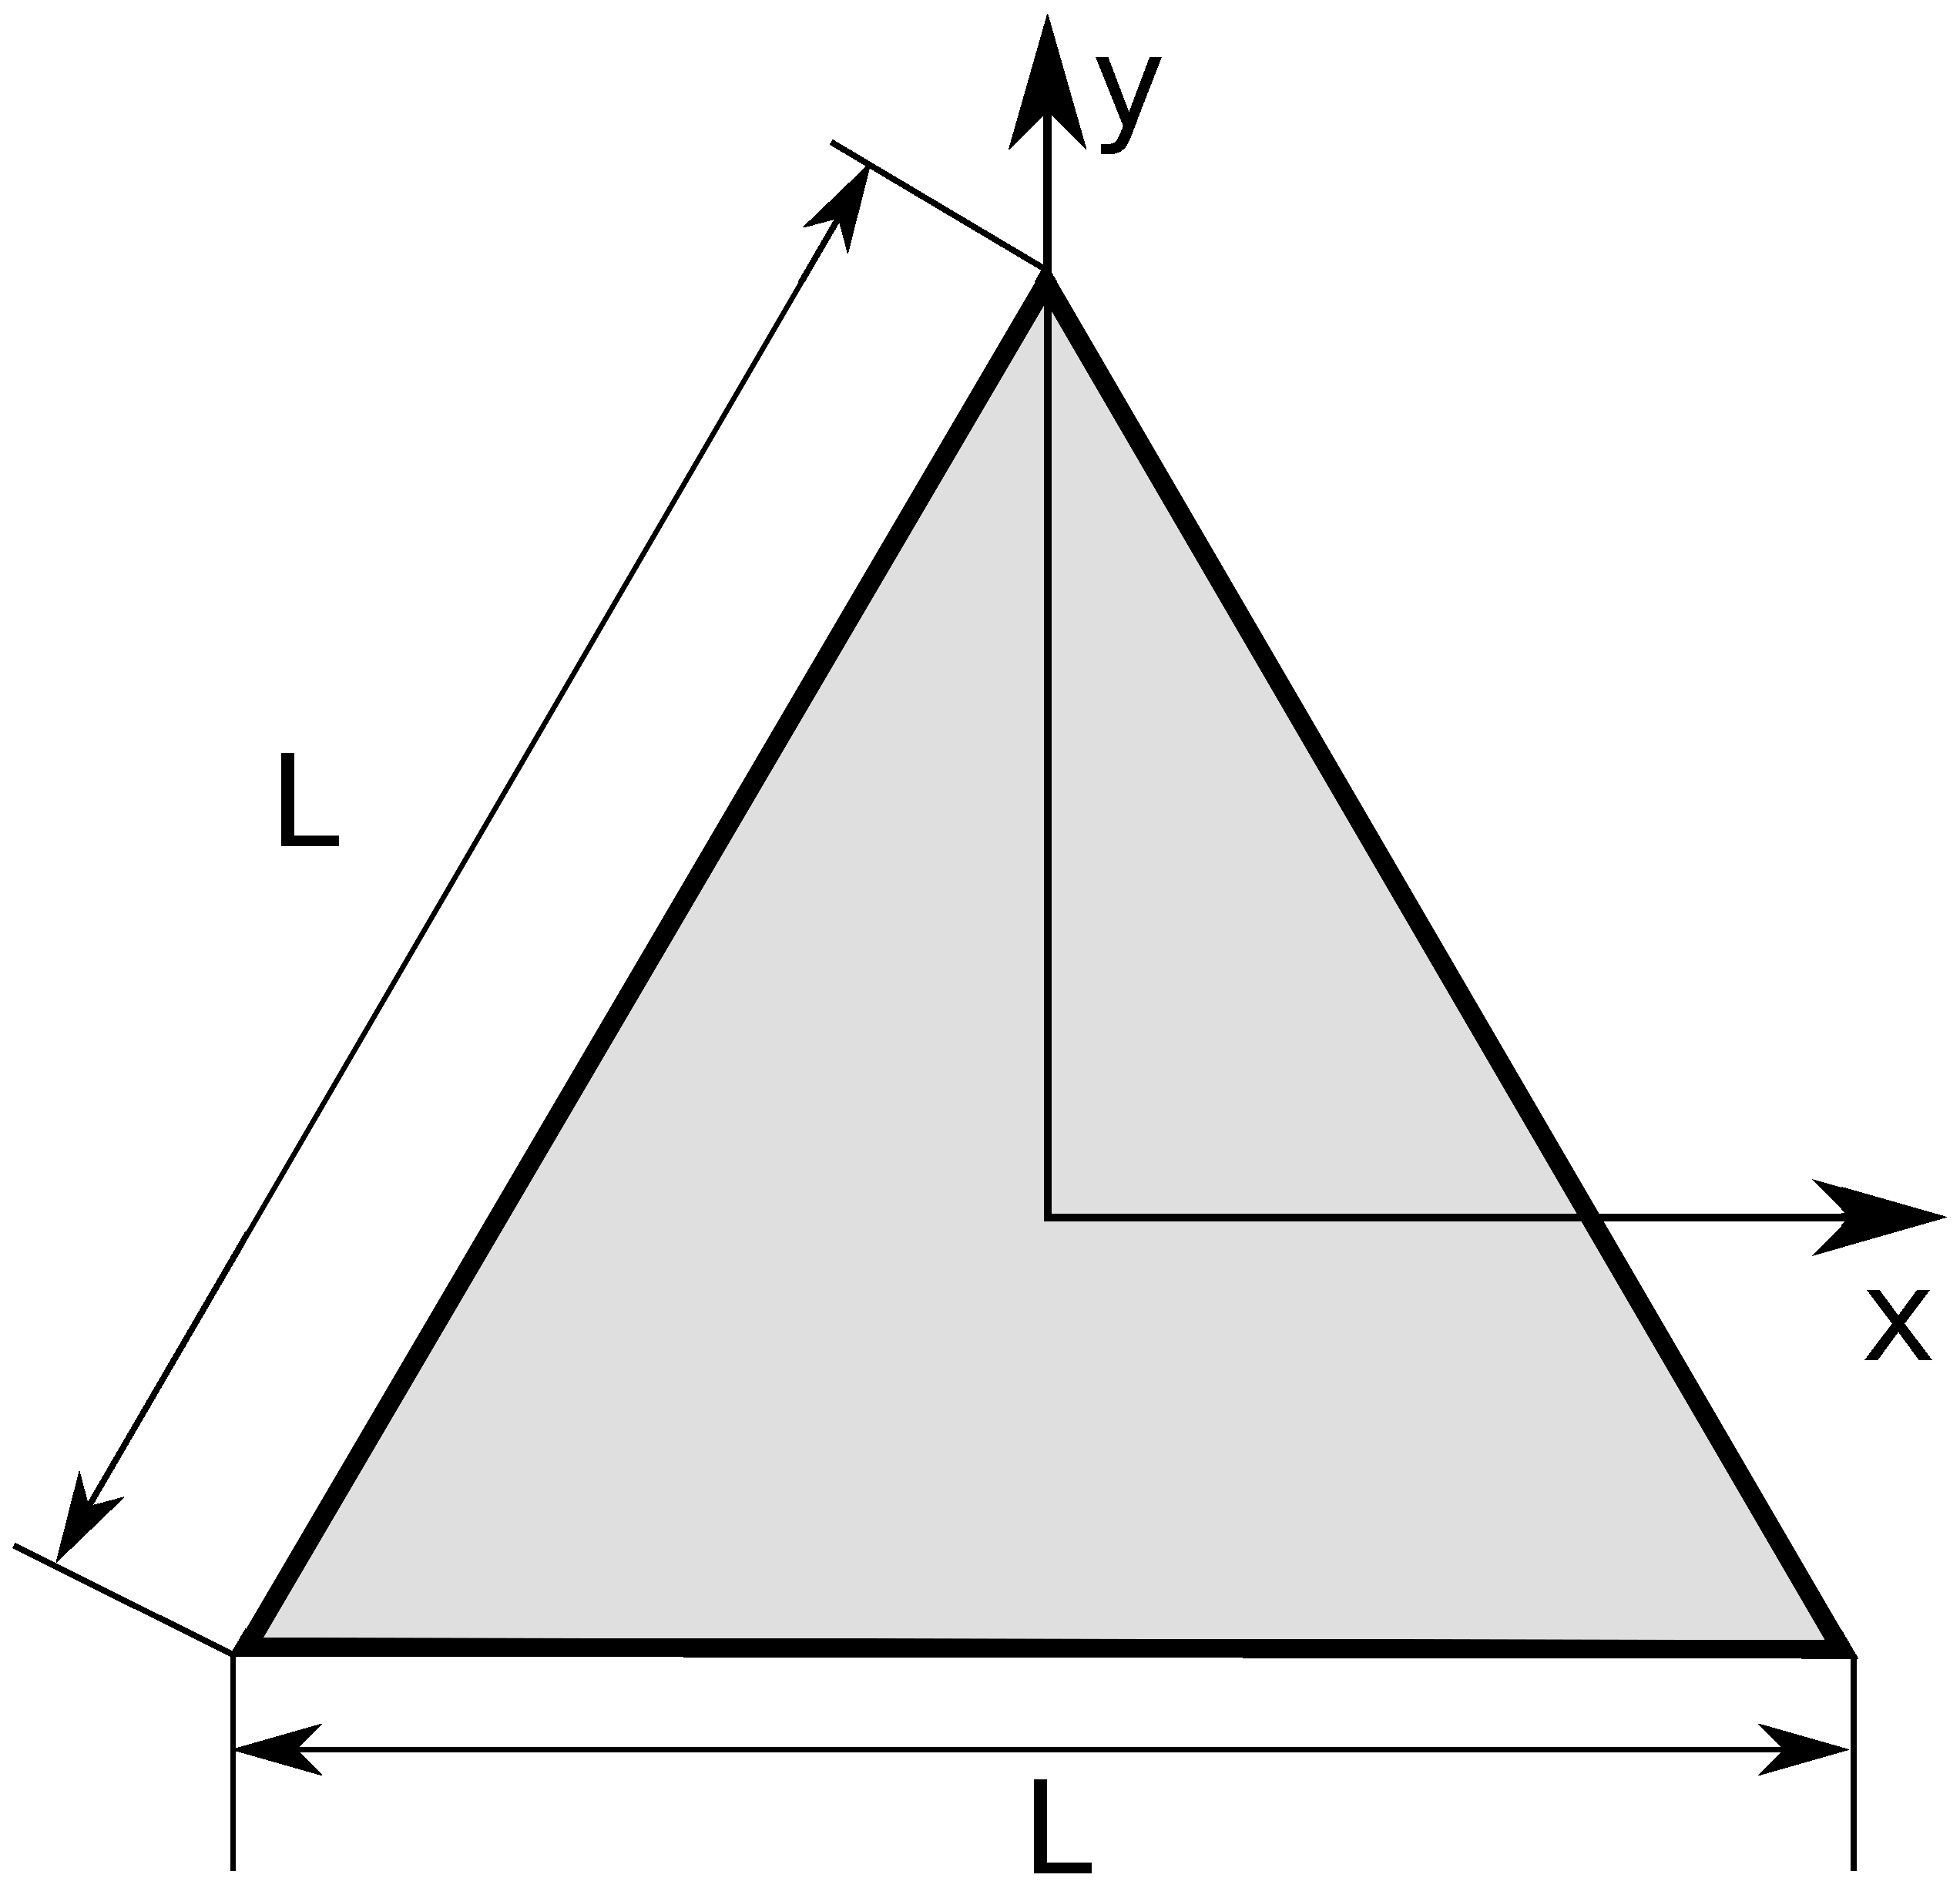
\includegraphics[width=5cm]{fig/cuts/Prism32dxy.eps}}
\hfill
\caption{Sketch of a Prism3.}
\label{fig:prism3}
\end{figure}

\FloatBarrier

\paragraph{Parameters}
\begin{itemize}
\item length $L$ of one side of the base, 
\item height $H$.
\end{itemize}

\paragraph{Properties}
\begin{itemize}
\item volume $V= \dfrac{\sqrt{3}}{4} H L^2$,
\item particle surface seen from above $S =\dfrac{\sqrt{3}}{4}L^2$.

\end{itemize}

\paragraph{Expression of the form factor}
\begin{align*}
F(\mathbf{q},L, H) &= \frac{2 \sqrt{3}}{q_x^2-3q_y^2}  \exp\left(-i q_y\frac{L}{2\sqrt{3}}\right)\left[\exp\left(i \sqrt{3} q_y \frac{L}{2} \right)-\cos\left(q_x \frac{L}{2}\right)-i \sqrt{3} q_y \frac{L}{2} \sinc\left(q_x \frac{L}{2}\right) \right] \\
  &
\times  H \sinc\left(q_z \frac{H}{2} \right) \exp\left(i q_z \frac{H}{2}\right),
\end{align*}
where $\sinc(x)=\sin(x)/x$ is the cardinal sine.

\paragraph{Syntax} \Code{FormFactorPrism3(length, height)}

\paragraph{Example}\mbox{}\\
Figure~\ref{fig:FFprism3Ex} shows the normalized intensity
$|F|^2/V^2$, computed with $L=10$~nm and \mbox{$H=13$~nm.}
\begin{figure}[ht]
\begin{center}
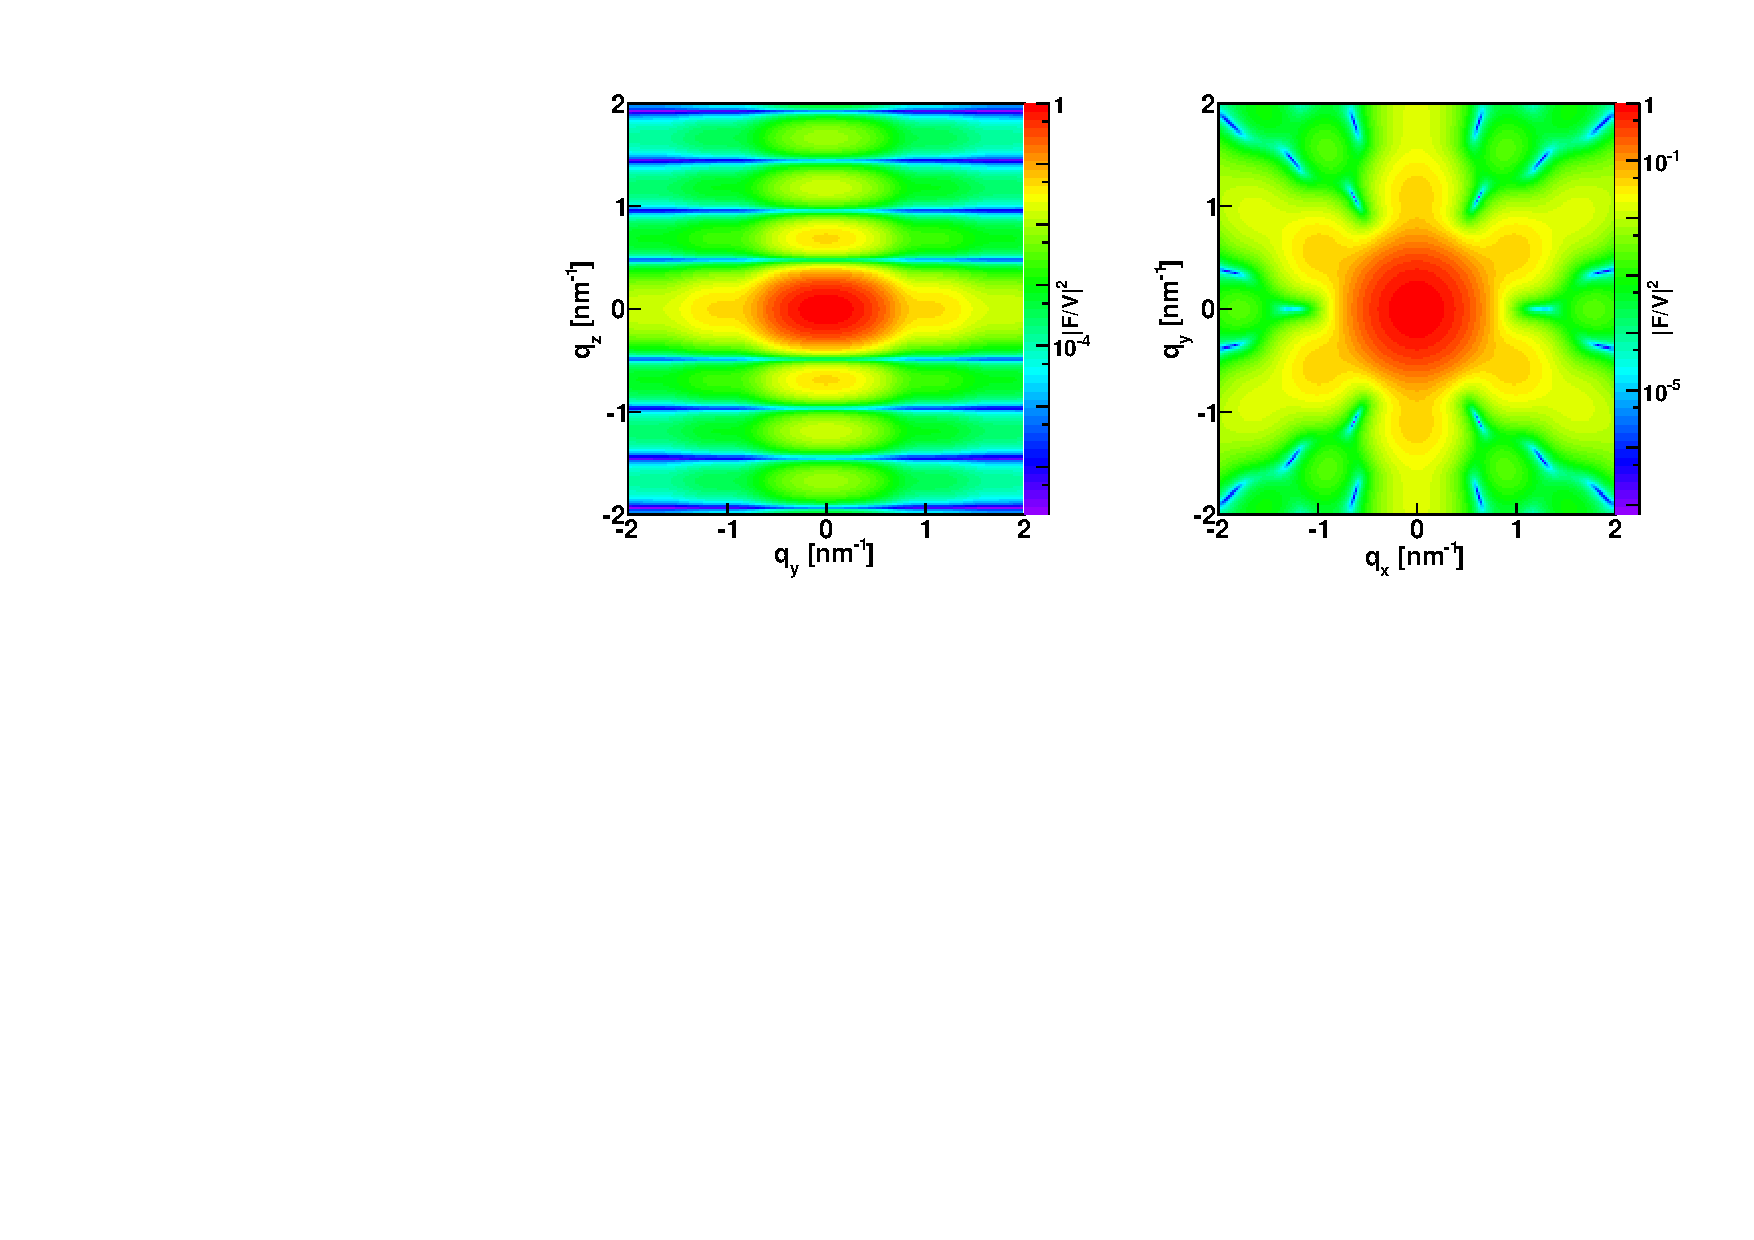
\includegraphics[angle=-90,width=\textwidth]{fig/ff/figffprism3.pdf}
\end{center}
\caption{Normalized intensity for the form factor of a Prism3
 plotted against ($q_y$, $q_z$) and  ($q_x$, $q_y$) and
  computed with \Code{FormFactorPrism3(10.*nanometer, 13.*nanometer)}.}
\label{fig:FFprism3Ex}
\end{figure}

\paragraph{References}
Agrees with \lq\lq Prism3\rq\rq ~form factor of \IsGISAXS~\cite{Laz02},
except for the definition of parameter $L= 2 R_{\rm{\Code{IsGISAXS}}}$.

%-------------------------------------------------------------------------------
\newpage
\subsubsection{Tetrahedron} \SecLabel{Tetrahedron}
  \index{Tetrahedron (form factor)}
  \index{Truncated tetrahedron (form factor)}
  \index{FormFactorTetrahedron@\Code{FormFactorTetrahedron}}
%-------------------------------------------------------------------------------
 
\paragraph{Real-space geometry}\mbox{}\\
This shape is a truncated tetrahedron as shown in fig.~\ref{fig:tetrahedron}.

\begin{figure}[ht]
\hfill
\subfigure[Side view]{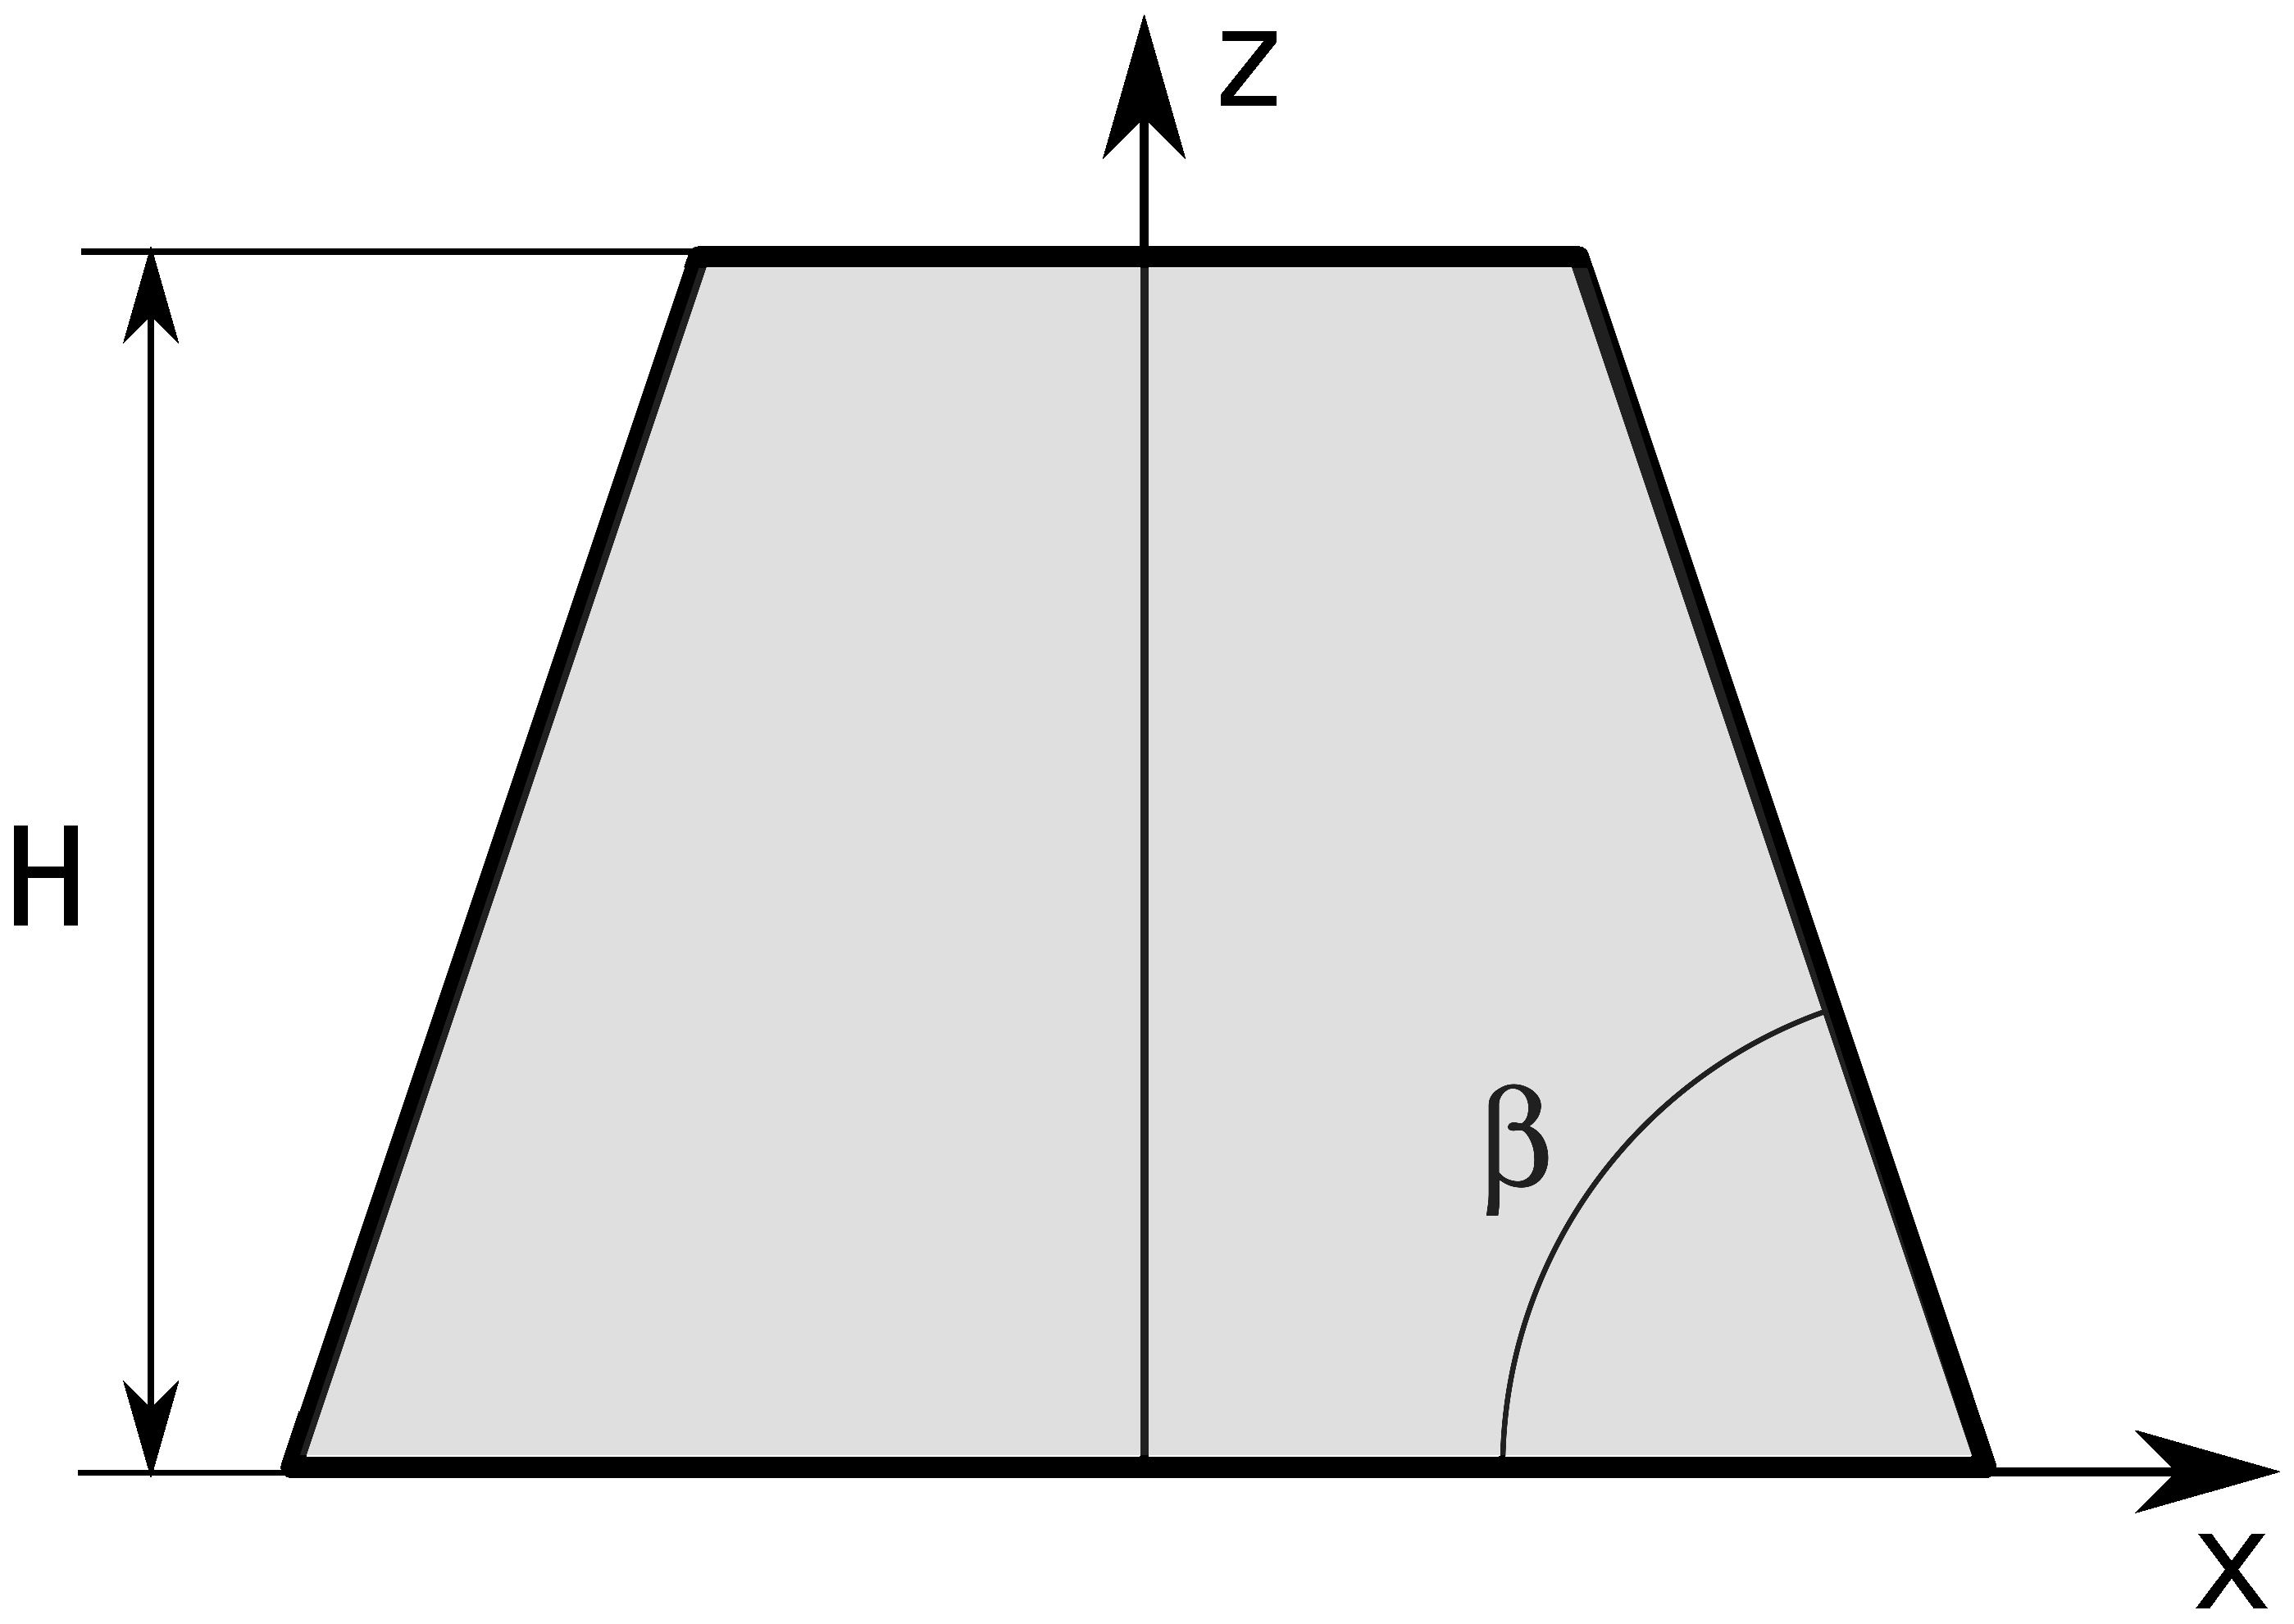
\includegraphics[width=5cm]{fig/cuts/Tetrahedron2dxz.eps}}
\hfill
\subfigure[Top view]{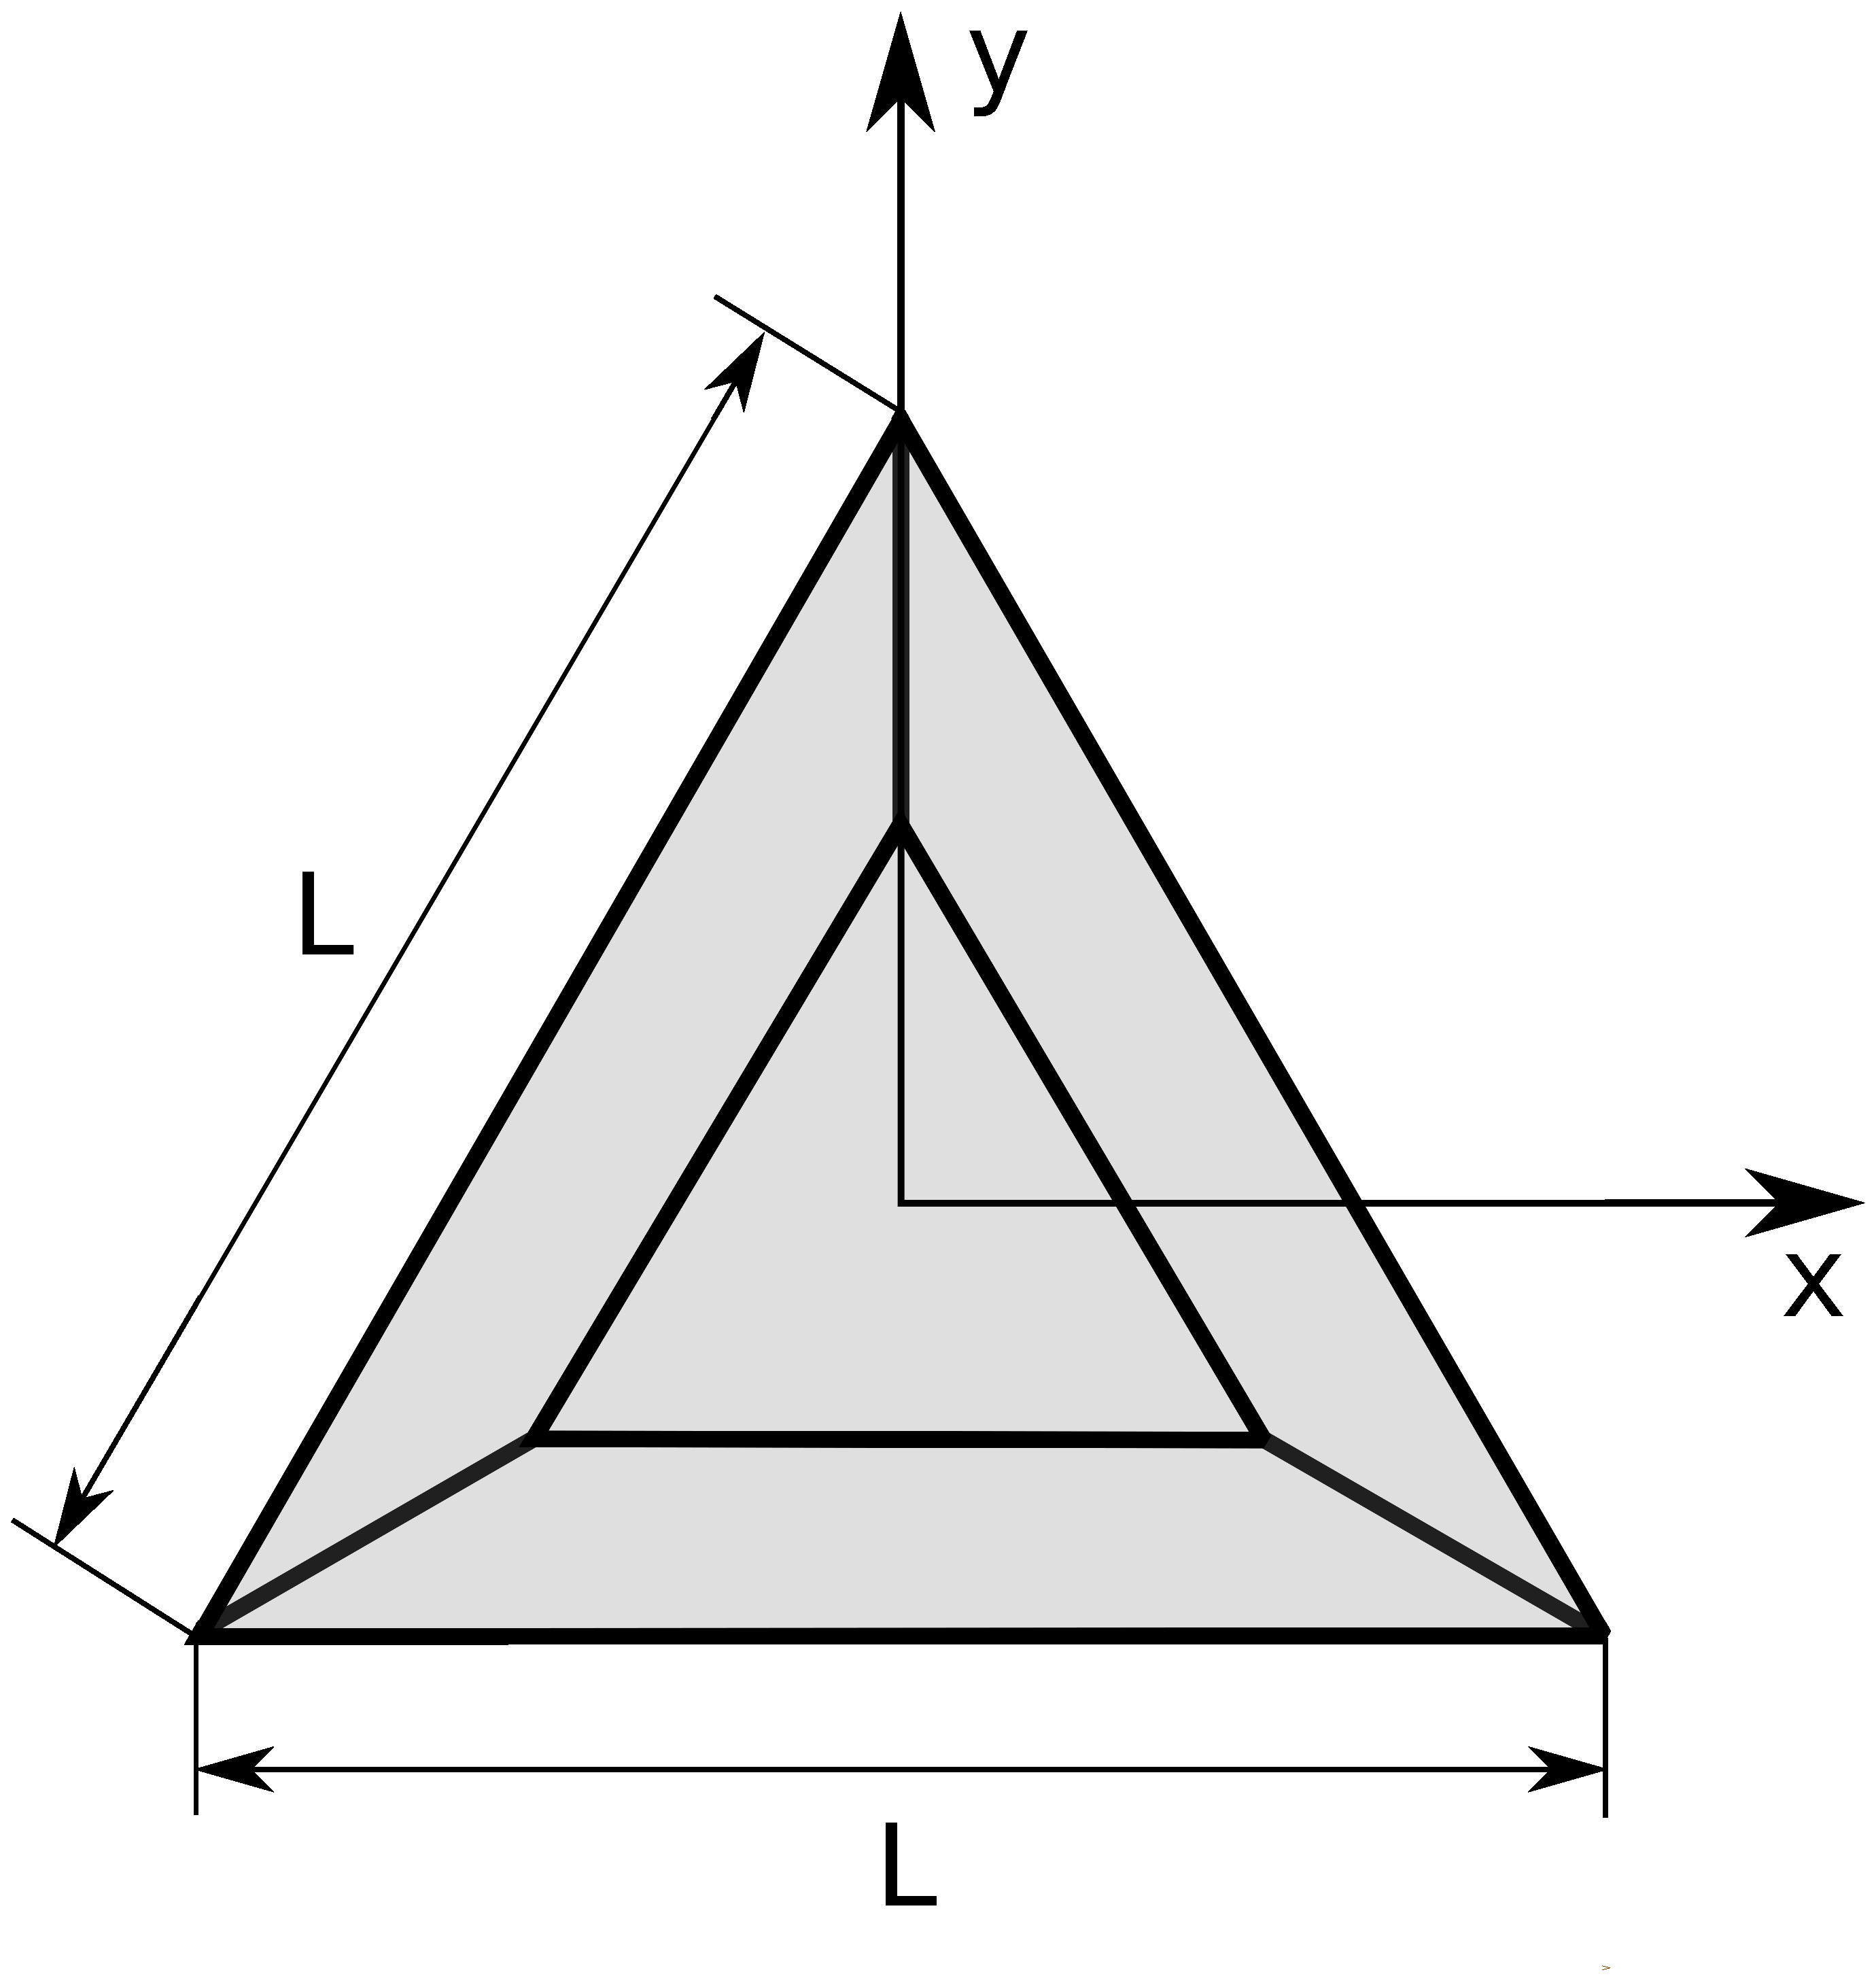
\includegraphics[width=5cm]{fig/cuts/Tetrahedron2dxy.eps}}
\hfill
\caption{Sketch of a Tetrahedron. The implementation of this shape uses angle
  $\alpha$, which is linked to $\beta$ via $\tan \alpha = 2 \tan 
  \beta$. $\alpha$ is the angle between the base and a side face and $\beta$
  the angle between the base and a side edge.}
\label{fig:tetrahedron}
\end{figure}

\FloatBarrier

\paragraph{Parameters}
\begin{itemize}
\item length of one side of the equilateral triangular base $L$,
\item height $H$,
\item angle $\alpha$ is the angle between the base and the
  side faces.
\end{itemize}

\paragraph{Restrictions on the parameters:} 
$\dfrac{H}{L}< \dfrac{\tan{\alpha}}{2\sqrt{3}}$.

\paragraph{Properties}
\begin{itemize}
\item volume $V= \dfrac{\tan(\alpha) L^3}{24} \left[1- \left(1 -
  \dfrac{2\sqrt{3} H}{L \tan(\alpha)} \right)^3\right]$,
\item particle surface seen from above $S =\dfrac{\sqrt{3}}{4}L^2$.
\end{itemize}

\paragraph{Expression of the form factor}

\begin{align*}
&F(\mathbf{q}, L, H, \alpha)=\frac{\sqrt{3}H}{q_x (q_x^2-3q_y^2)}
\exp\left(i\frac{q_z L\tan (\alpha)}{2\sqrt{3}}\right) \times \\
&\Big\{2q_x \exp(iq_3 D)\sinc(q_3 H) - (q_x +\sqrt{3}q_y)
\exp(iq_1 D)\sinc(q_1 H) -(q_x-\sqrt{3}q_y)\exp(-iq_2
D)\sinc(q_2 H) \Big\}, 
\end{align*}
with $\sinc(x)=\sin(x)/x$,
\begin{equation*}
q_1  =\frac{1}{2}\left[\frac{q_x\sqrt{3} -q_y}{\tan \alpha}-q_z \right],
\quad q_2 = \frac{1}{2}\left[\frac{q_x\sqrt{3} +q_y}{\tan \alpha}+q_z
\right], \quad 
q_3 = \frac{q_y}{\tan \alpha} -\frac{q_z}{2}, \quad D = \frac{L \tan \alpha}{\sqrt{3}} -H.
\end{equation*}

\paragraph{Syntax} \Code{FormFactorTetrahedron(length, height, alpha)}

\paragraph{Example}\mbox{}\\
Figure~\ref{fig:FFtetrahEx} shows the normalized intensity
$|F|^2/V^2$, computed with $L=15$~nm, $H=6$~nm and $\alpha =60
^{\circ}$.

\begin{figure}[ht]
\begin{center}
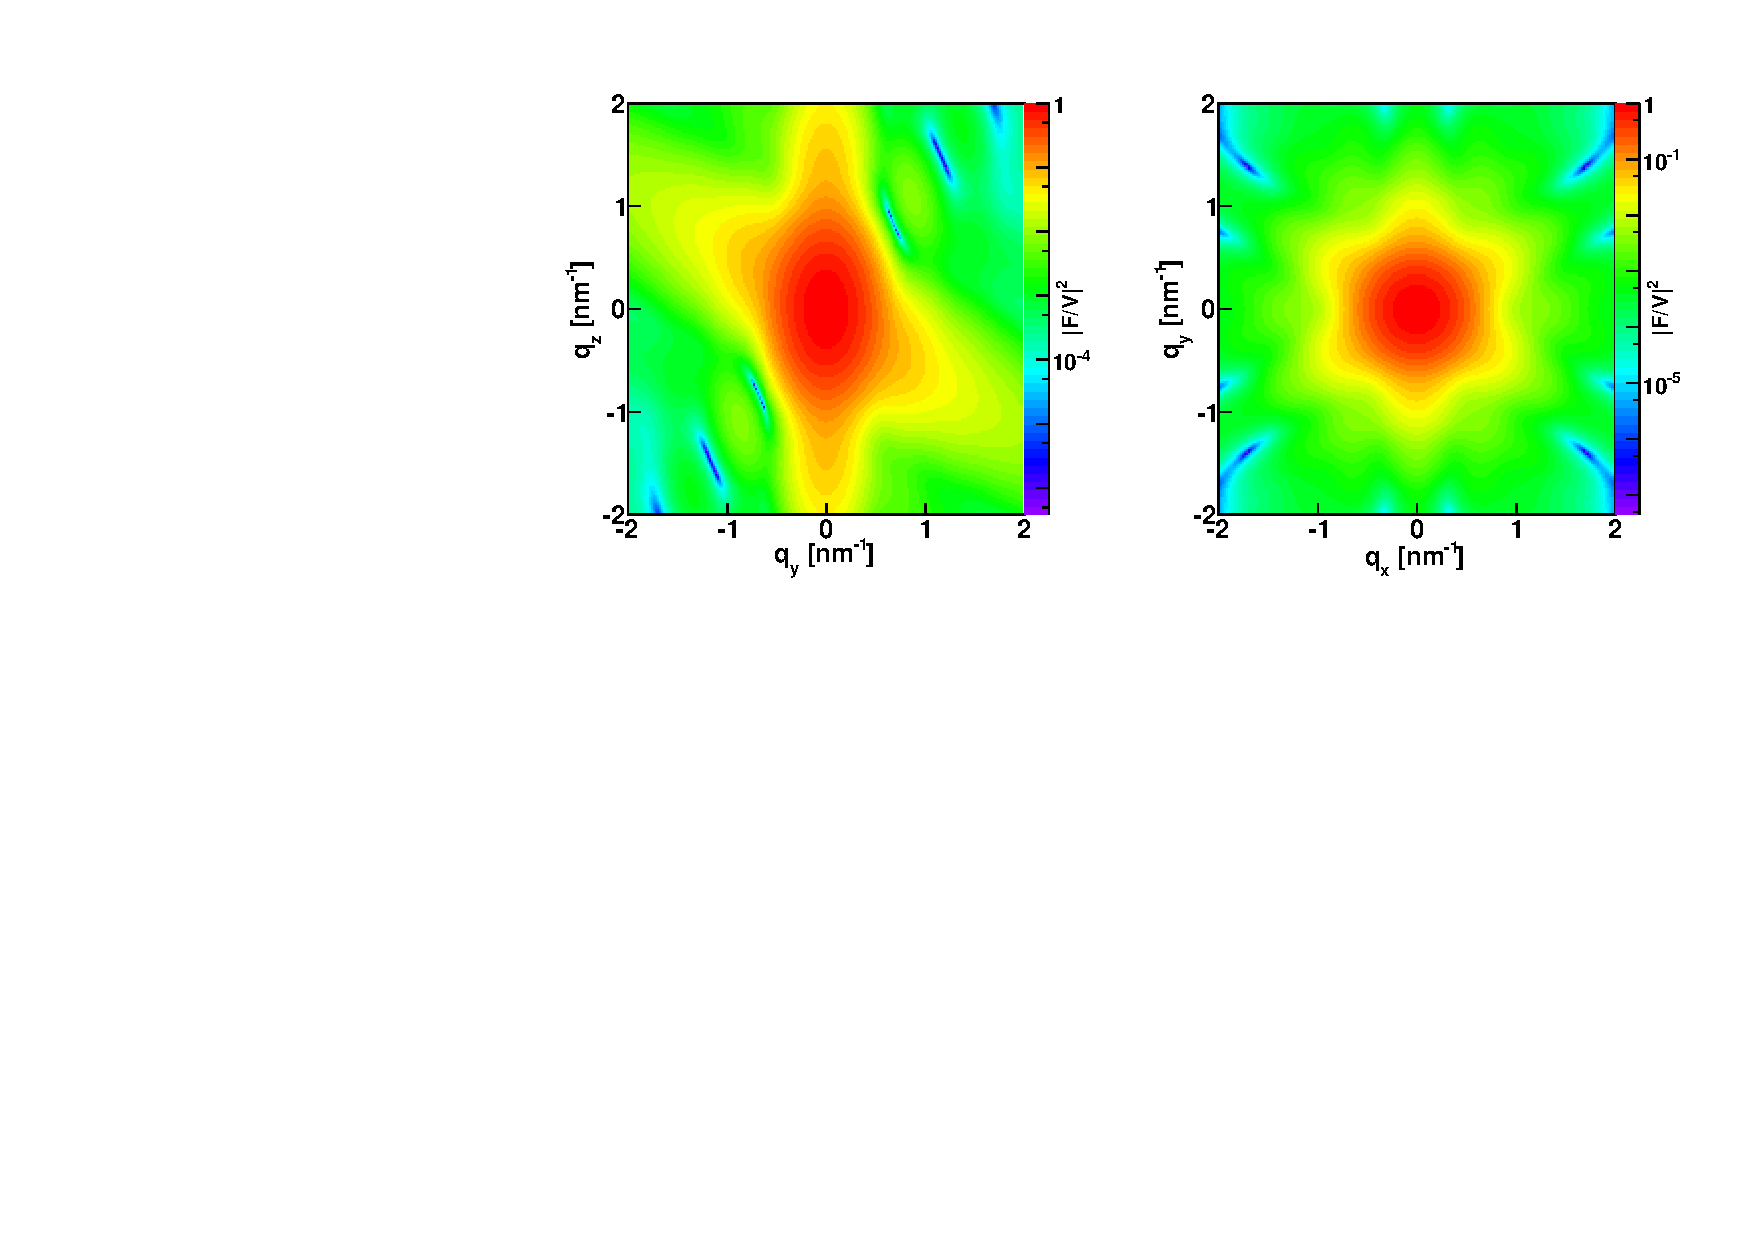
\includegraphics[angle=-90,width=\textwidth]{fig/ff/figfftetrahedron.pdf}
\end{center}
\caption{Normalized intensity for the form factor of a Tetrahedron
  plotted against ($q_y$, $q_z$) and  ($q_x$, $q_y$) and
  computed with \Code{FormFactorTetrahedron(15.*nanometer, 6.*nanometer, 60.*degree)}.}
\label{fig:FFtetrahEx}
\end{figure}

\paragraph{References}
??

%-------------------------------------------------------------------------------
\newpage
\subsubsection{Prism6 (hexagonal)} \SecLabel{Prism6}
  \index{Prism (form factor)!hexagonal (Prism6)}
  \index{FormFactorPrism6@\Code{FormFactorPrism6}}
%-------------------------------------------------------------------------------

\paragraph{Real-space geometry}\mbox{}\\
This shape is an hexagonal prism (see fig.~\ref{fig:prism6}).

\begin{figure}[ht]
\hfill
\subfigure[Side view]{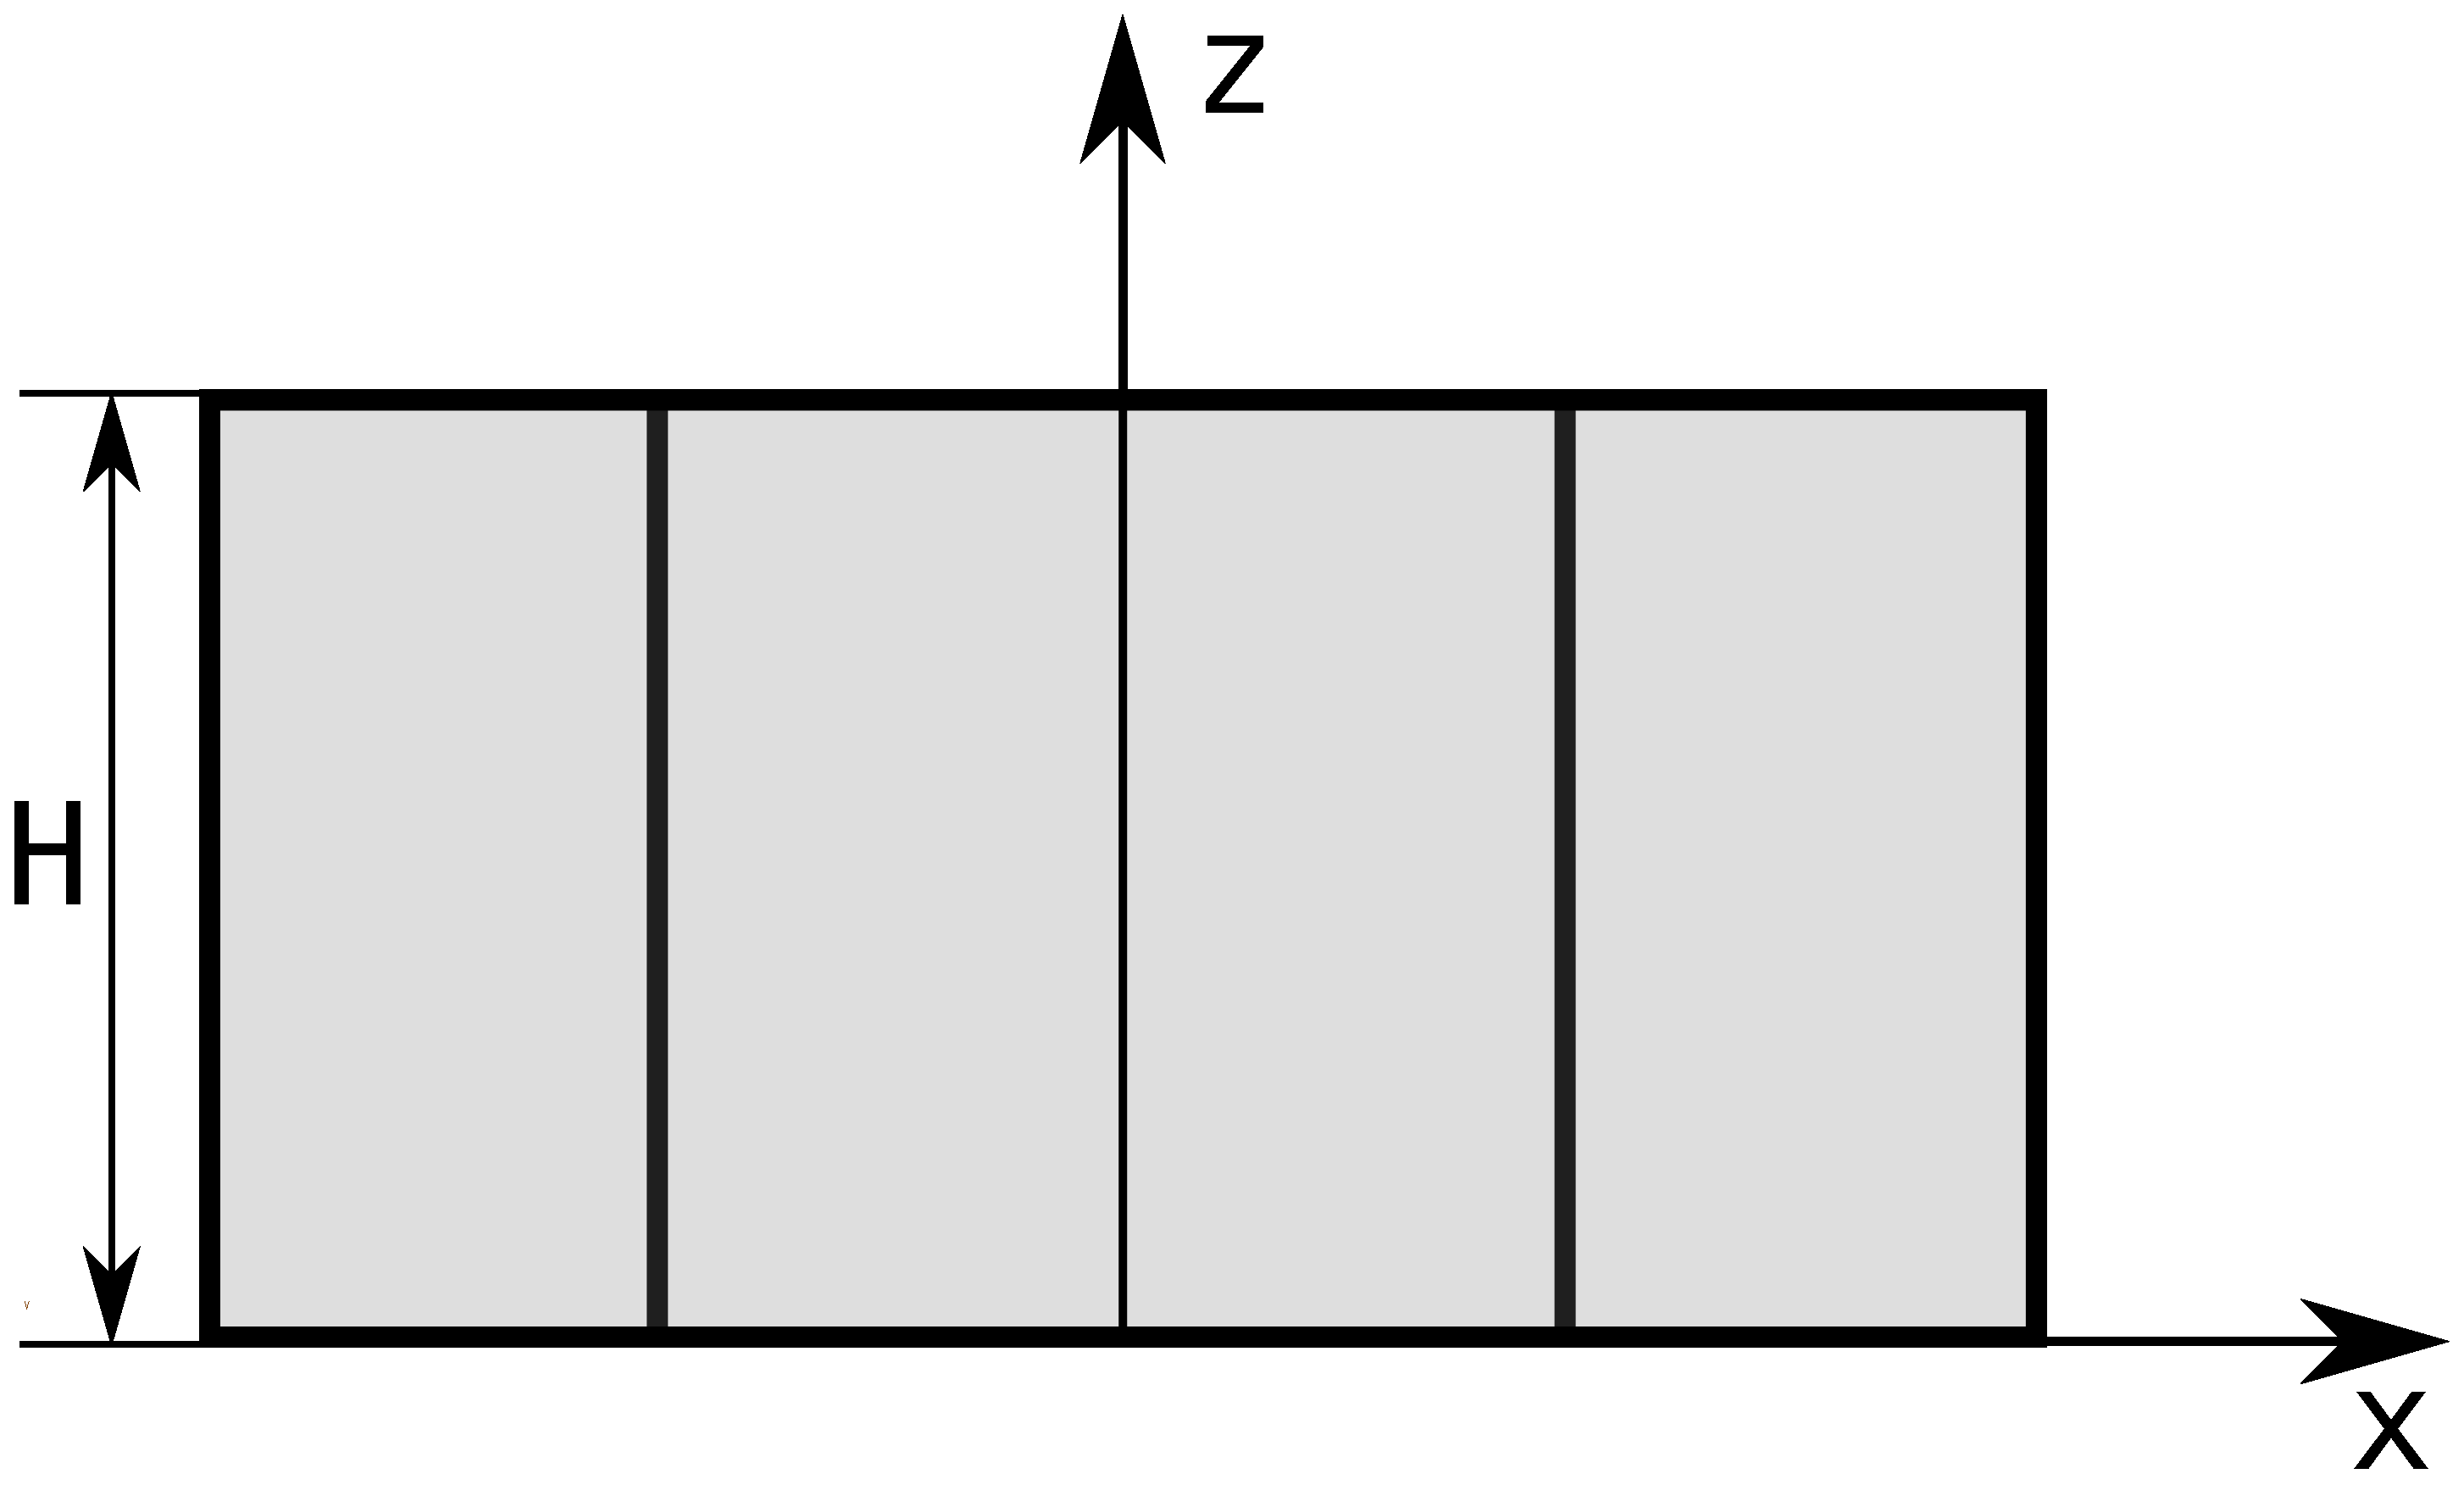
\includegraphics[width=5cm]{fig/cuts/Prism62dxz.eps}}
\hfill
\subfigure[Top view]{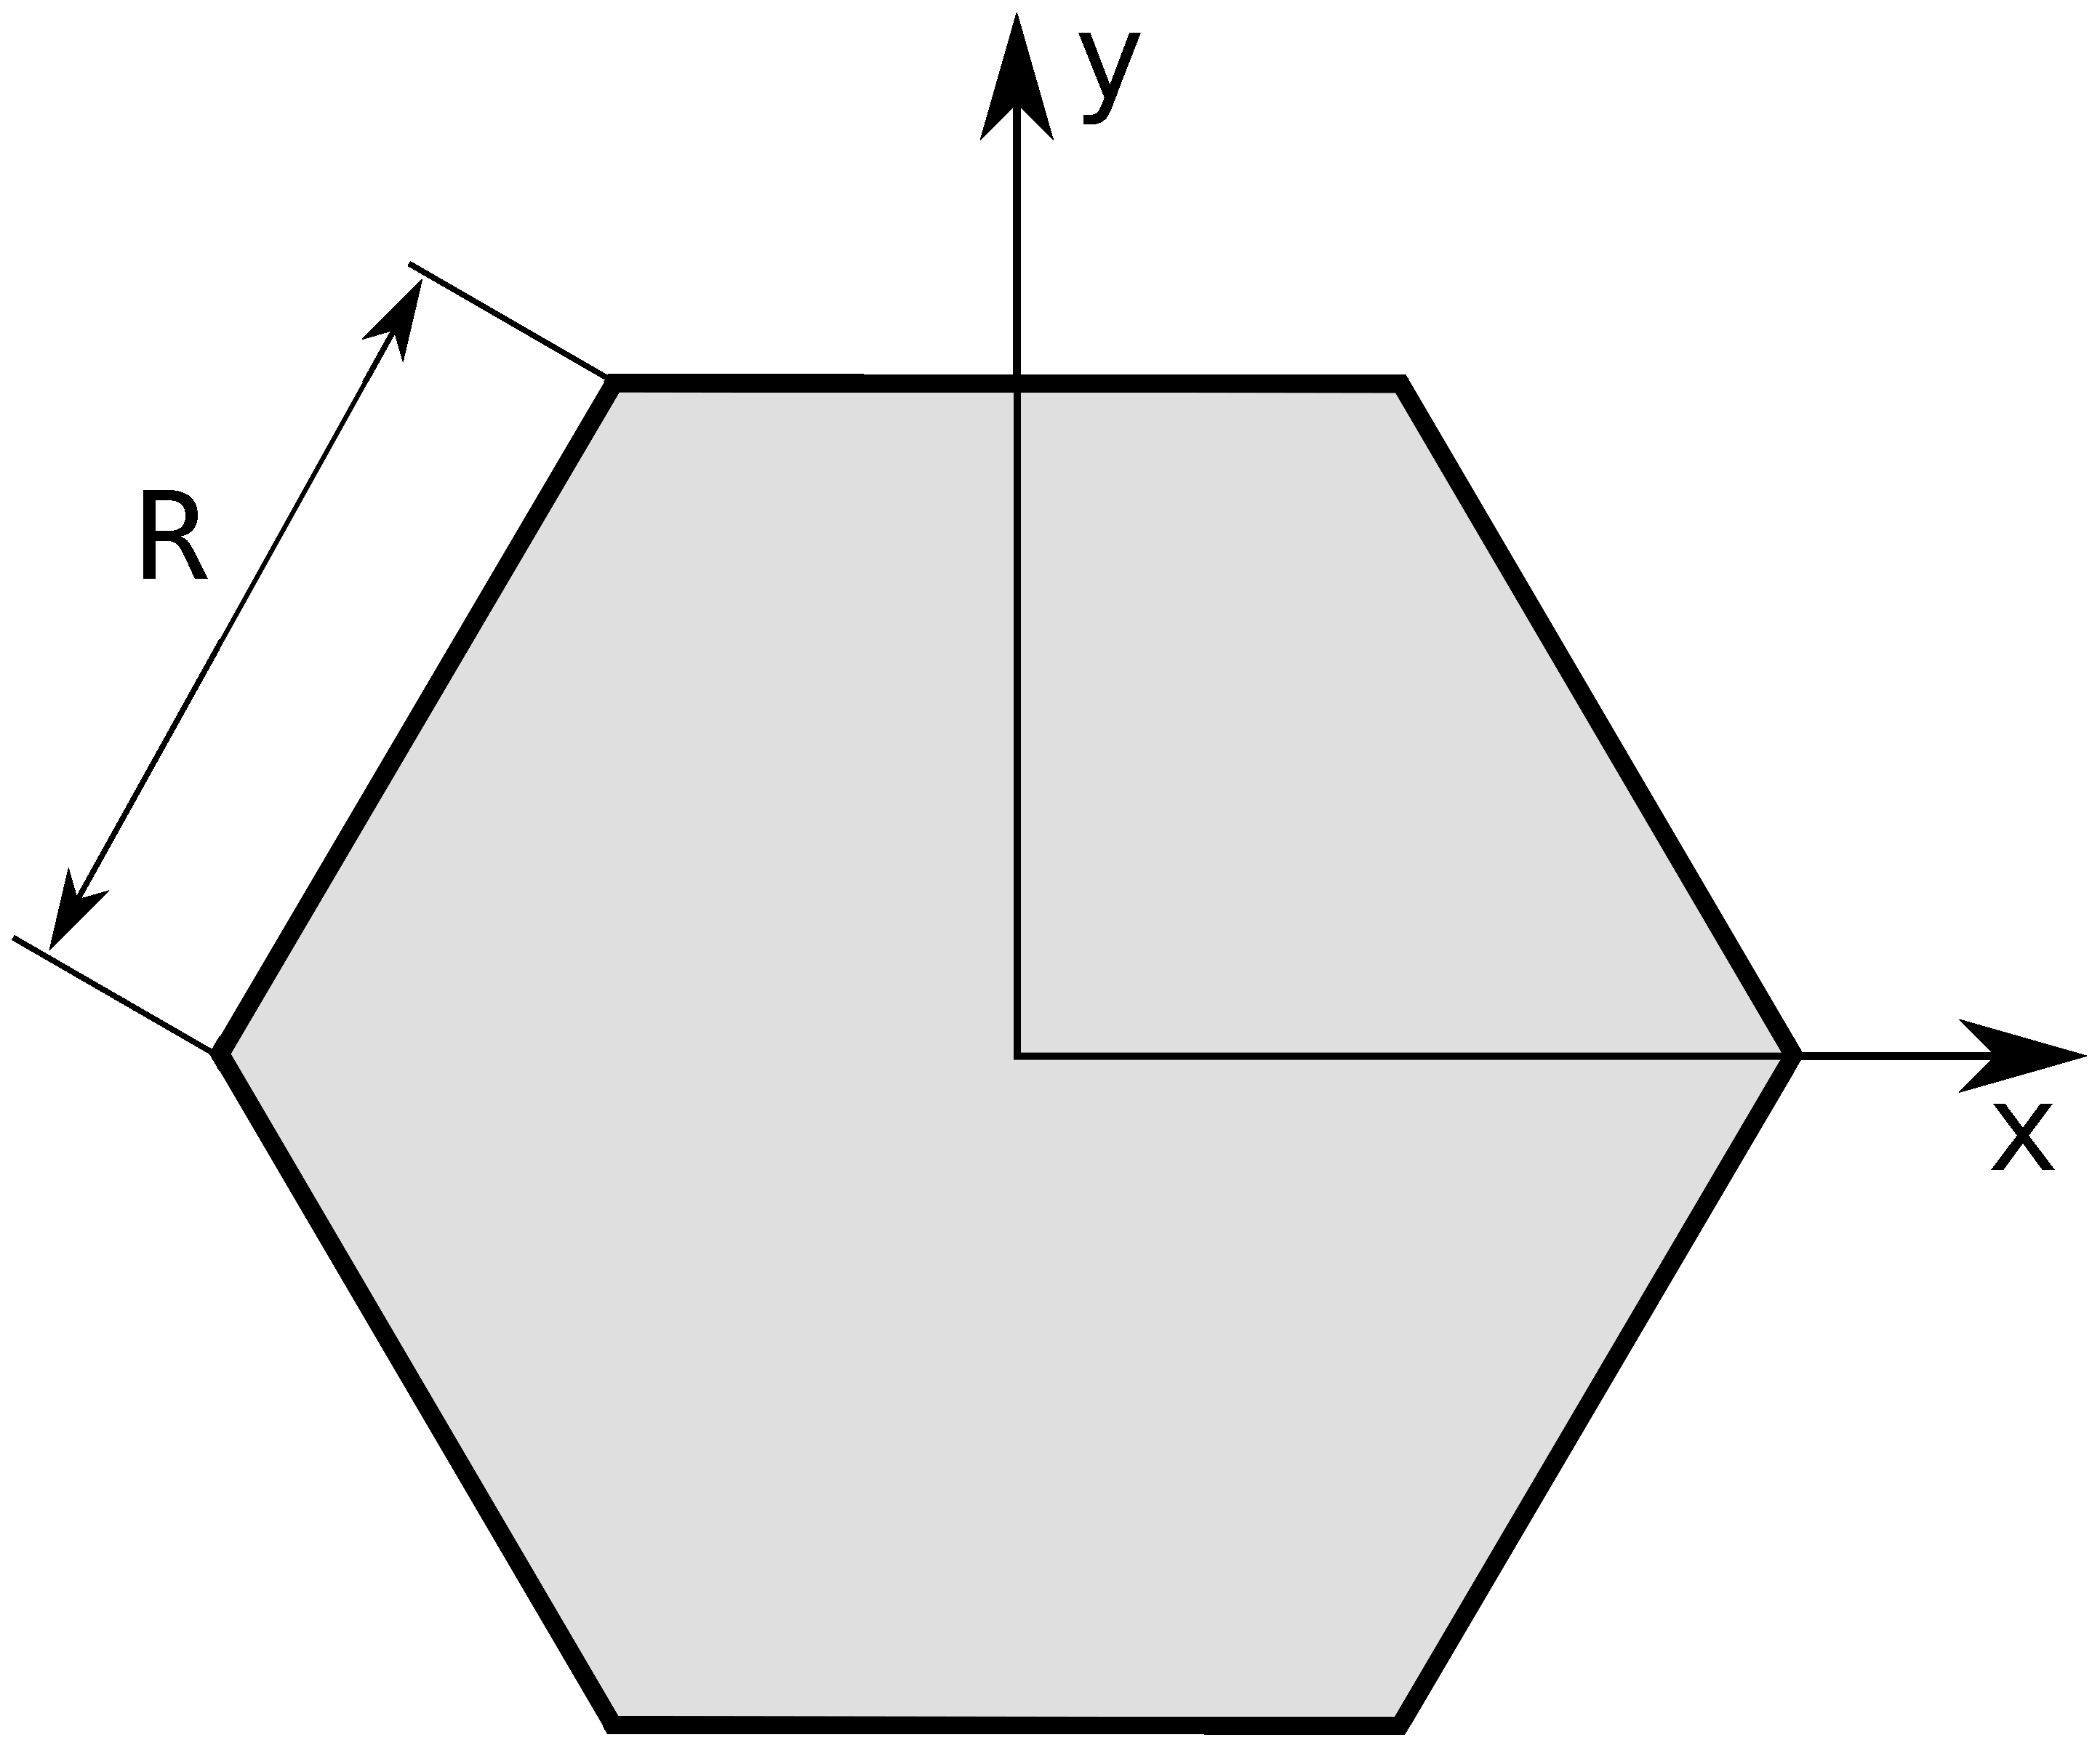
\includegraphics[width=5cm]{fig/cuts/Prism62dxy.eps}}
\hfill
\caption{Sketch of a Prism6.}
\label{fig:prism6}
\end{figure}

\FloatBarrier

\paragraph{Parameters}
\begin{itemize}
\item radius of the hexagonal base $R$,
\item height $H$.
\end{itemize}

\paragraph{Properties}
\begin{itemize}
\item volume $V = \dfrac{3\sqrt{3}}{2}H R^2$,
\item particle surface seen from above $S =\dfrac{3\sqrt{3}R^2}{2}$.
\end{itemize}

\paragraph{Expression of the form factor}
\begin{align*}
F(\mathbf{q}, R, H) &= \frac{4H\sqrt{3}}{3q_y^2 - q_x^2}
\sinc\left(q_z\frac{H}{2}\right) \exp\left(-i q_z\frac{ H}{2}\right)\times\\
&\left\{\frac{3q_y^2R^2}{4} \sinc\left(\frac{q_x
  R}{2}\right)\sinc\left(\frac{\sqrt{3}q_yR }{2}\right)+ \cos(q_x R)-\cos\left(q_y
\frac{\sqrt{3}R}{2}\right) \cos\left(\frac{q_x R}{2}\right)\right\},
\end{align*}
with $\sinc(x)=\sin(x)/x$.

\paragraph{Syntax} \Code{FormFactorPrism6(radius, height)} 

\newpage

\paragraph{Example}\mbox{}\\
Figure~\ref{fig:FFprism6Ex} shows the normalized intensity
$|F|^2/V^2$, computed with $R=5$~nm and \mbox{$H=11$~nm.}

\begin{figure}[ht]
\begin{center}
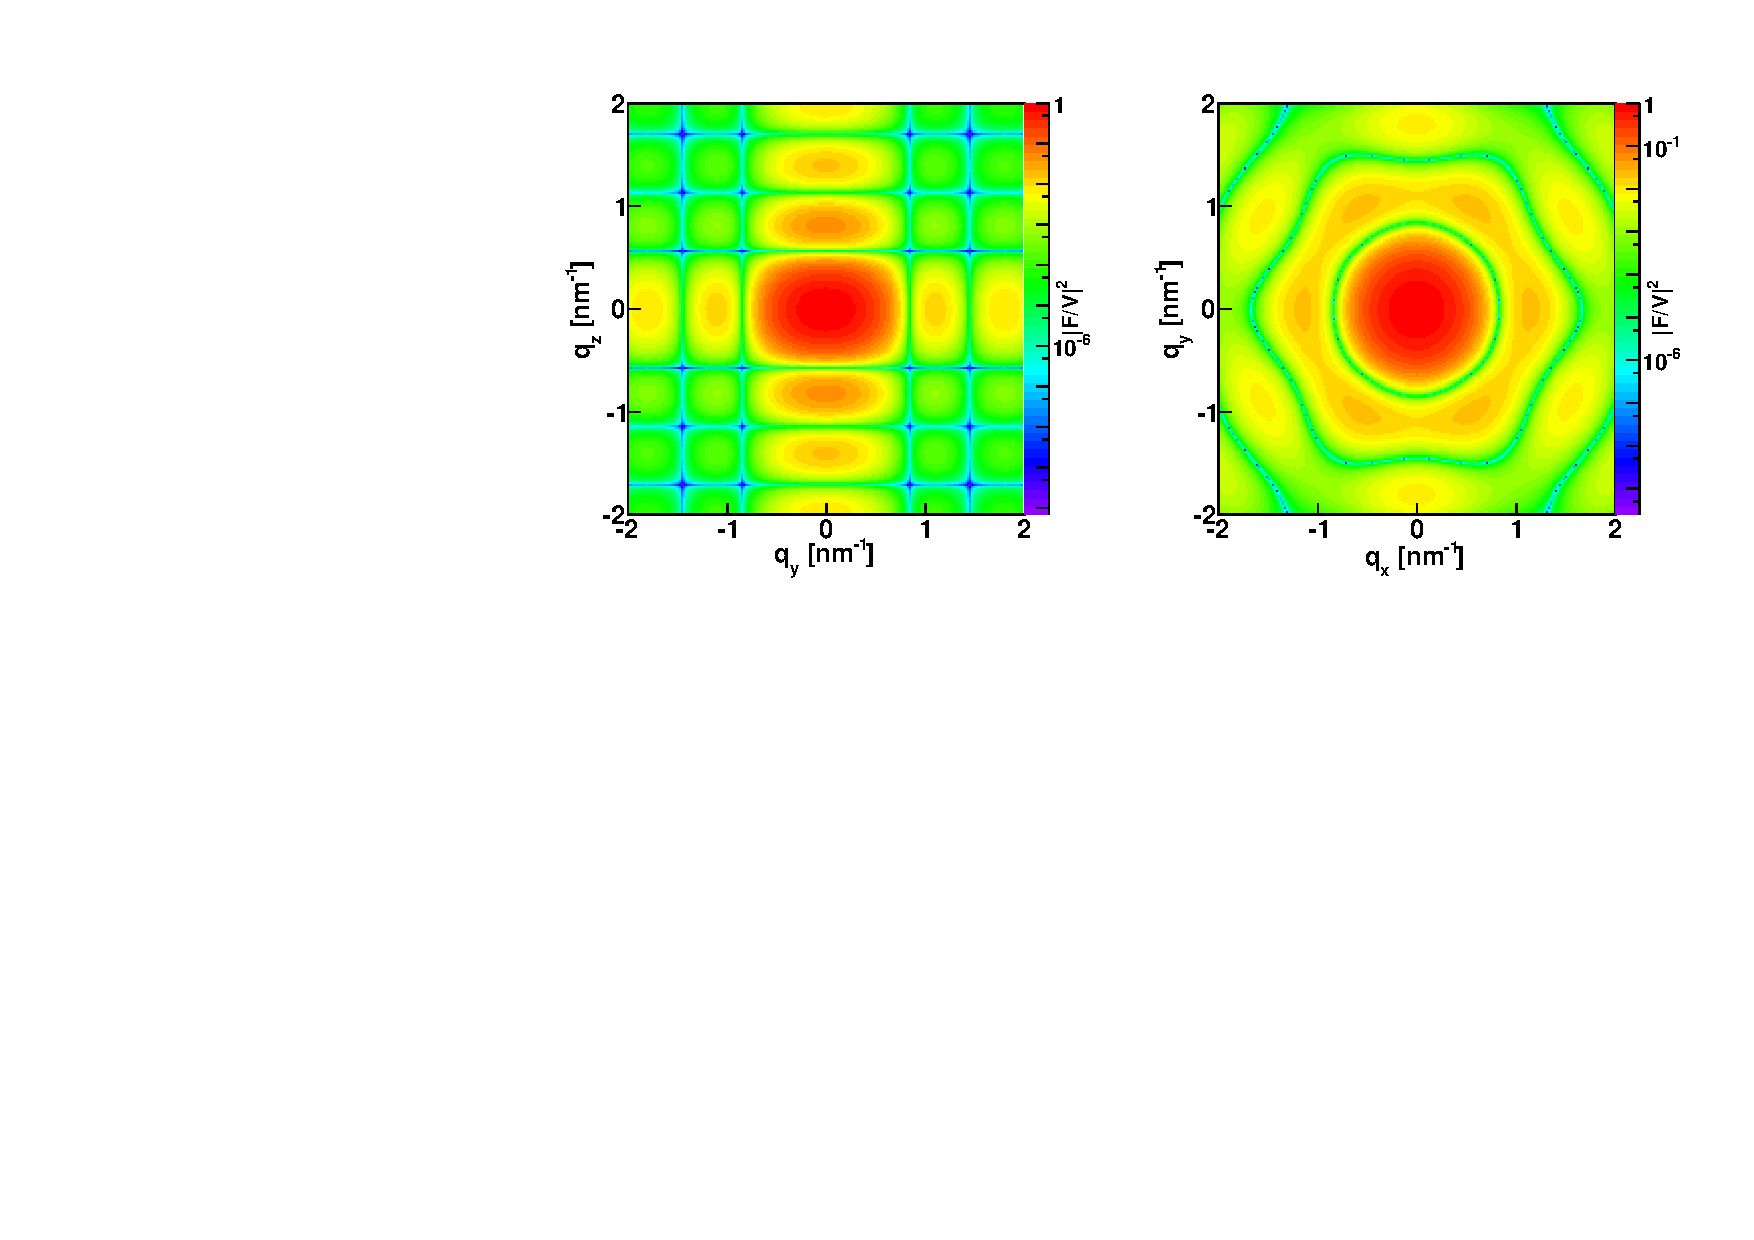
\includegraphics[angle=-90,width=\textwidth]{fig/ff/figffprism6.pdf}
\end{center}
\caption{Normalized intensity for the form factor of a Prism6 plotted against ($q_y$, $q_z$) and ($q_x$, $q_y$) and computed with \Code{FormFactorPrism6(5.*nanometer, 11.*nanometer)}.}
\label{fig:FFprism6Ex}
\end{figure}

\paragraph{References}
Agrees with \lq\lq Prism6\rq\rq ~form factor of \IsGISAXS~\cite{Laz02},
except for different parametrization,
and for a factor $H$ missing in the \Code{IsGISAXS} manual. 

%-------------------------------------------------------------------------------
\newpage
\subsubsection{Cone6 (hexagonal)} \SecLabel{Cone6}
  \index{Cone (form factor)!hexagonal (Cone6)}
  \index{Pyramid (form factor)!hexagonal (Cone6)}
  \index{Truncated pyramid (form factor)!hexagonal (Cone6)}
  \index{FormFactorCone6@\Code{FormFactorCone6}}
%-------------------------------------------------------------------------------

\paragraph{Real-space geometry}\mbox{}\\
It is a truncated hexagonal pyramid (see fig.~\ref{fig:cone6}). 

\begin{figure}[ht]
\hfill
\subfigure[Side view]{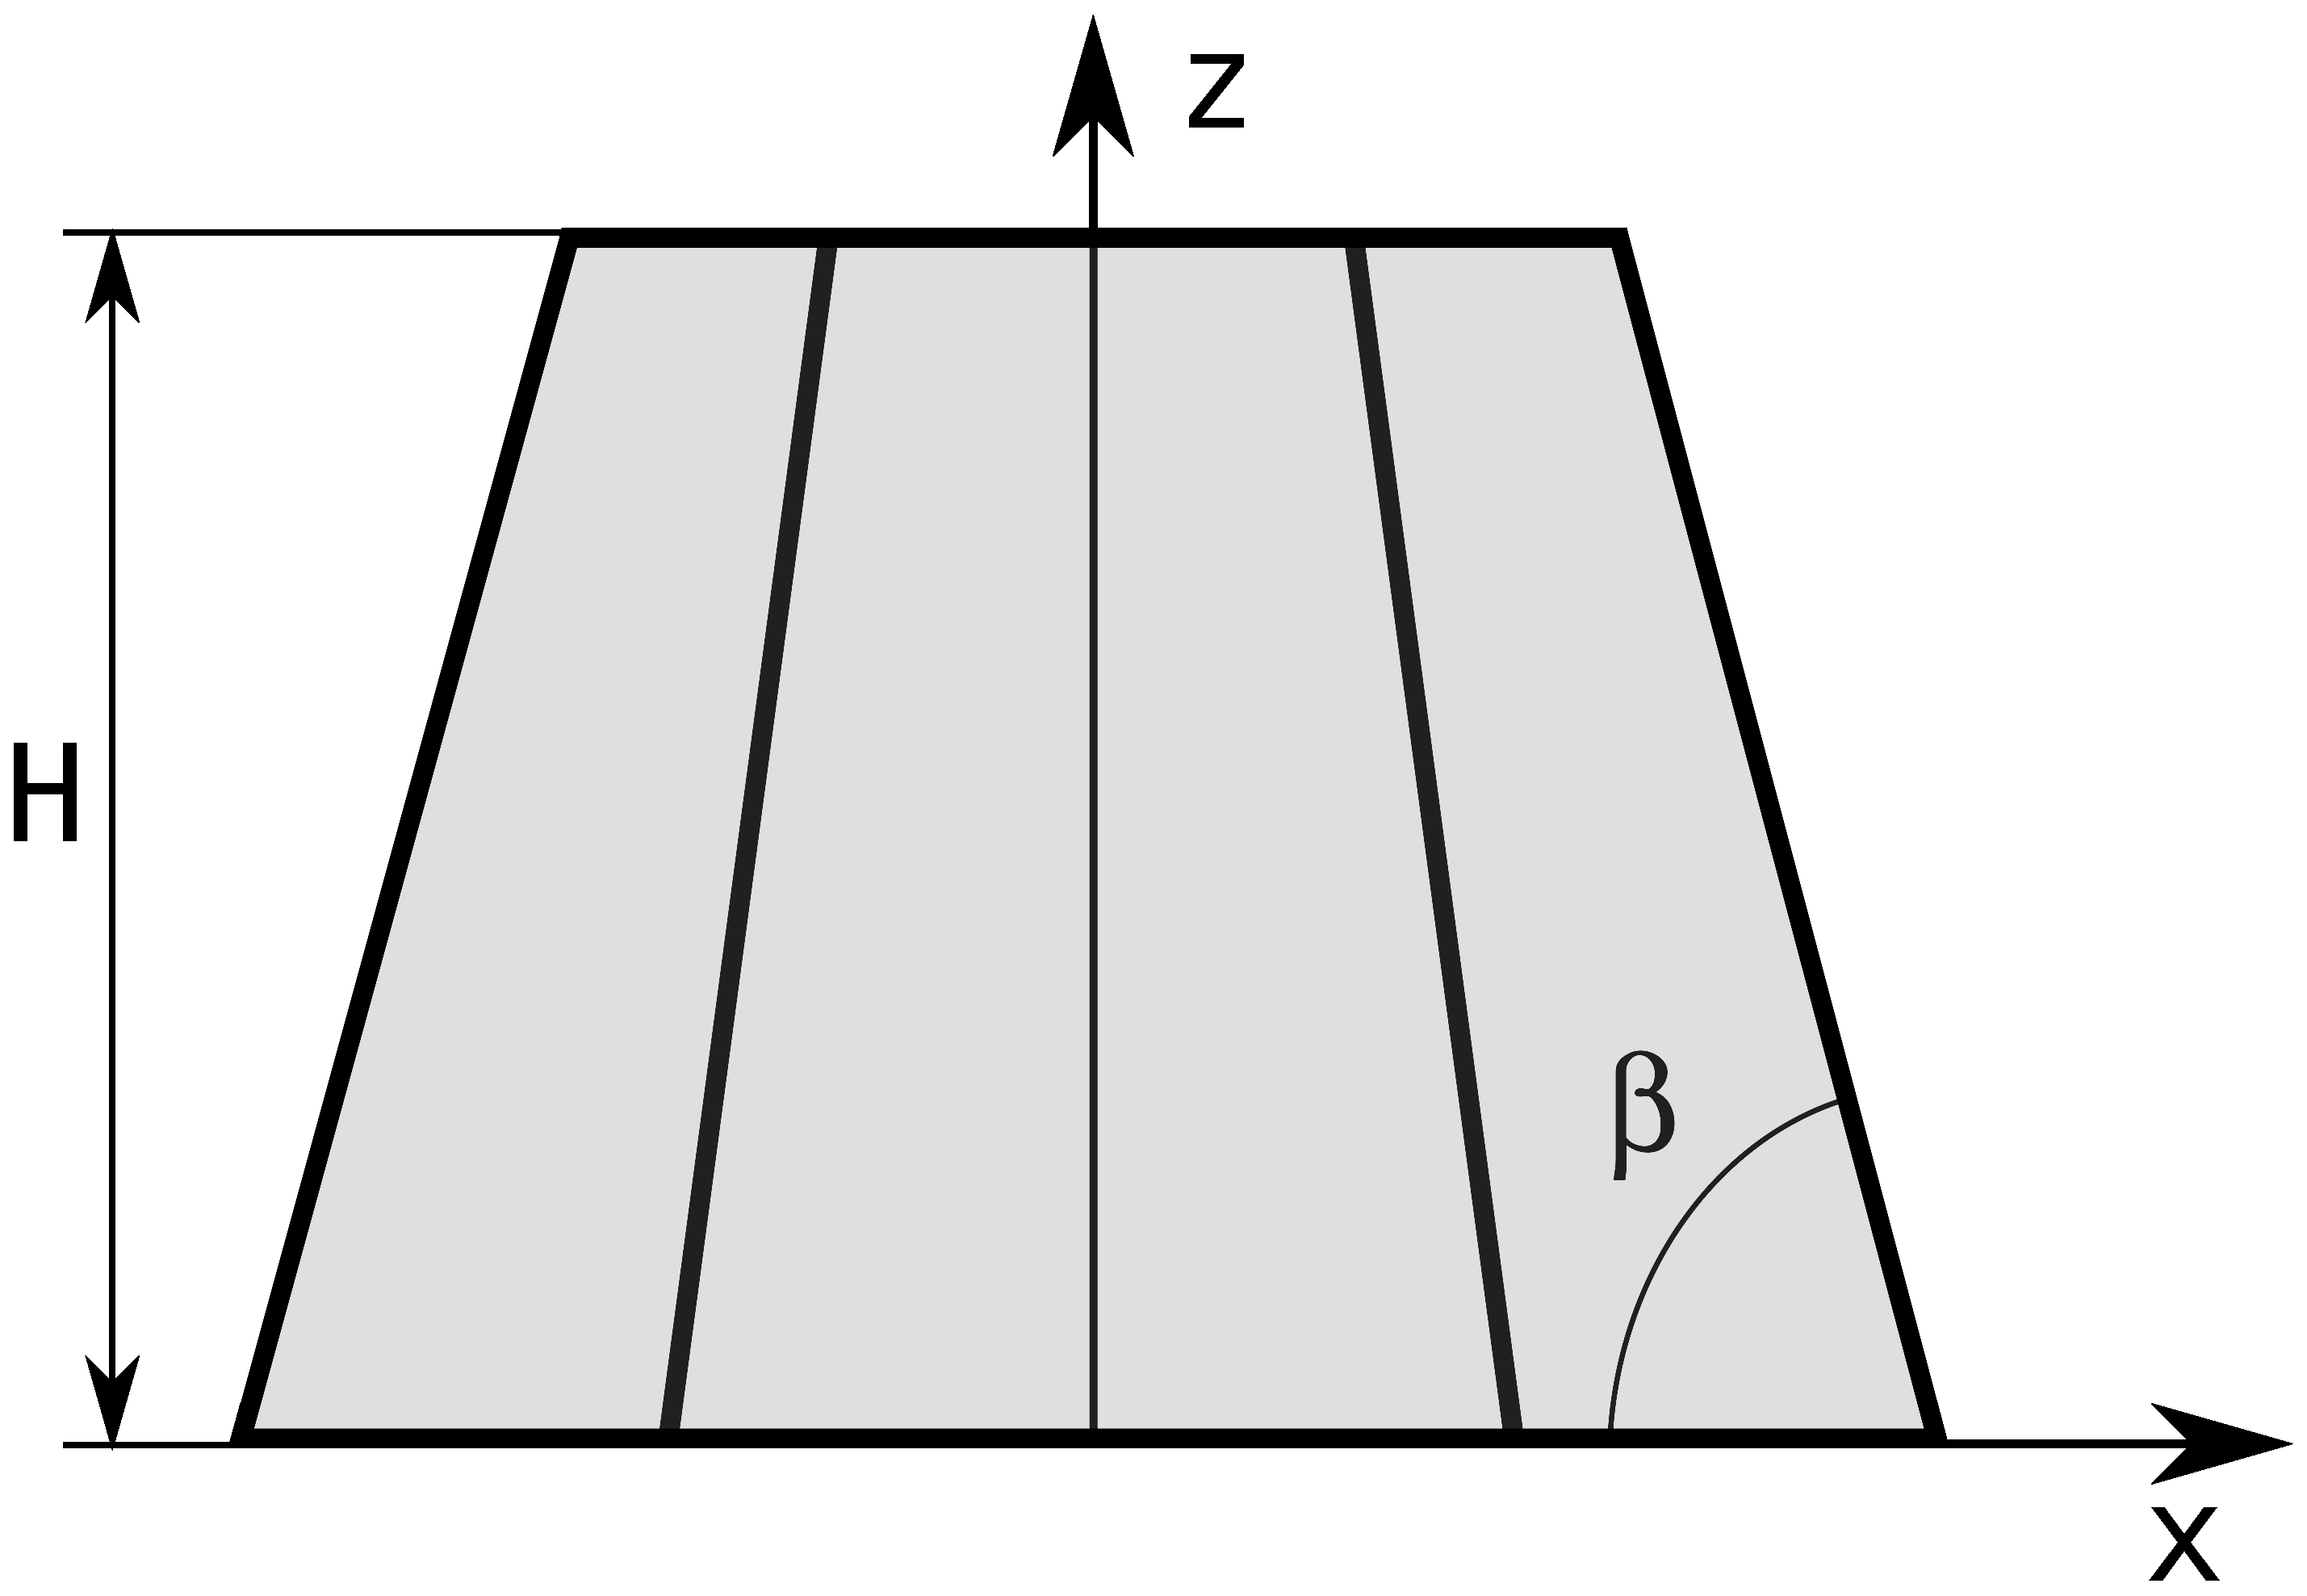
\includegraphics[width=5cm]{fig/cuts/Cone62dxz.eps}}
\hfill
\subfigure[Top view]{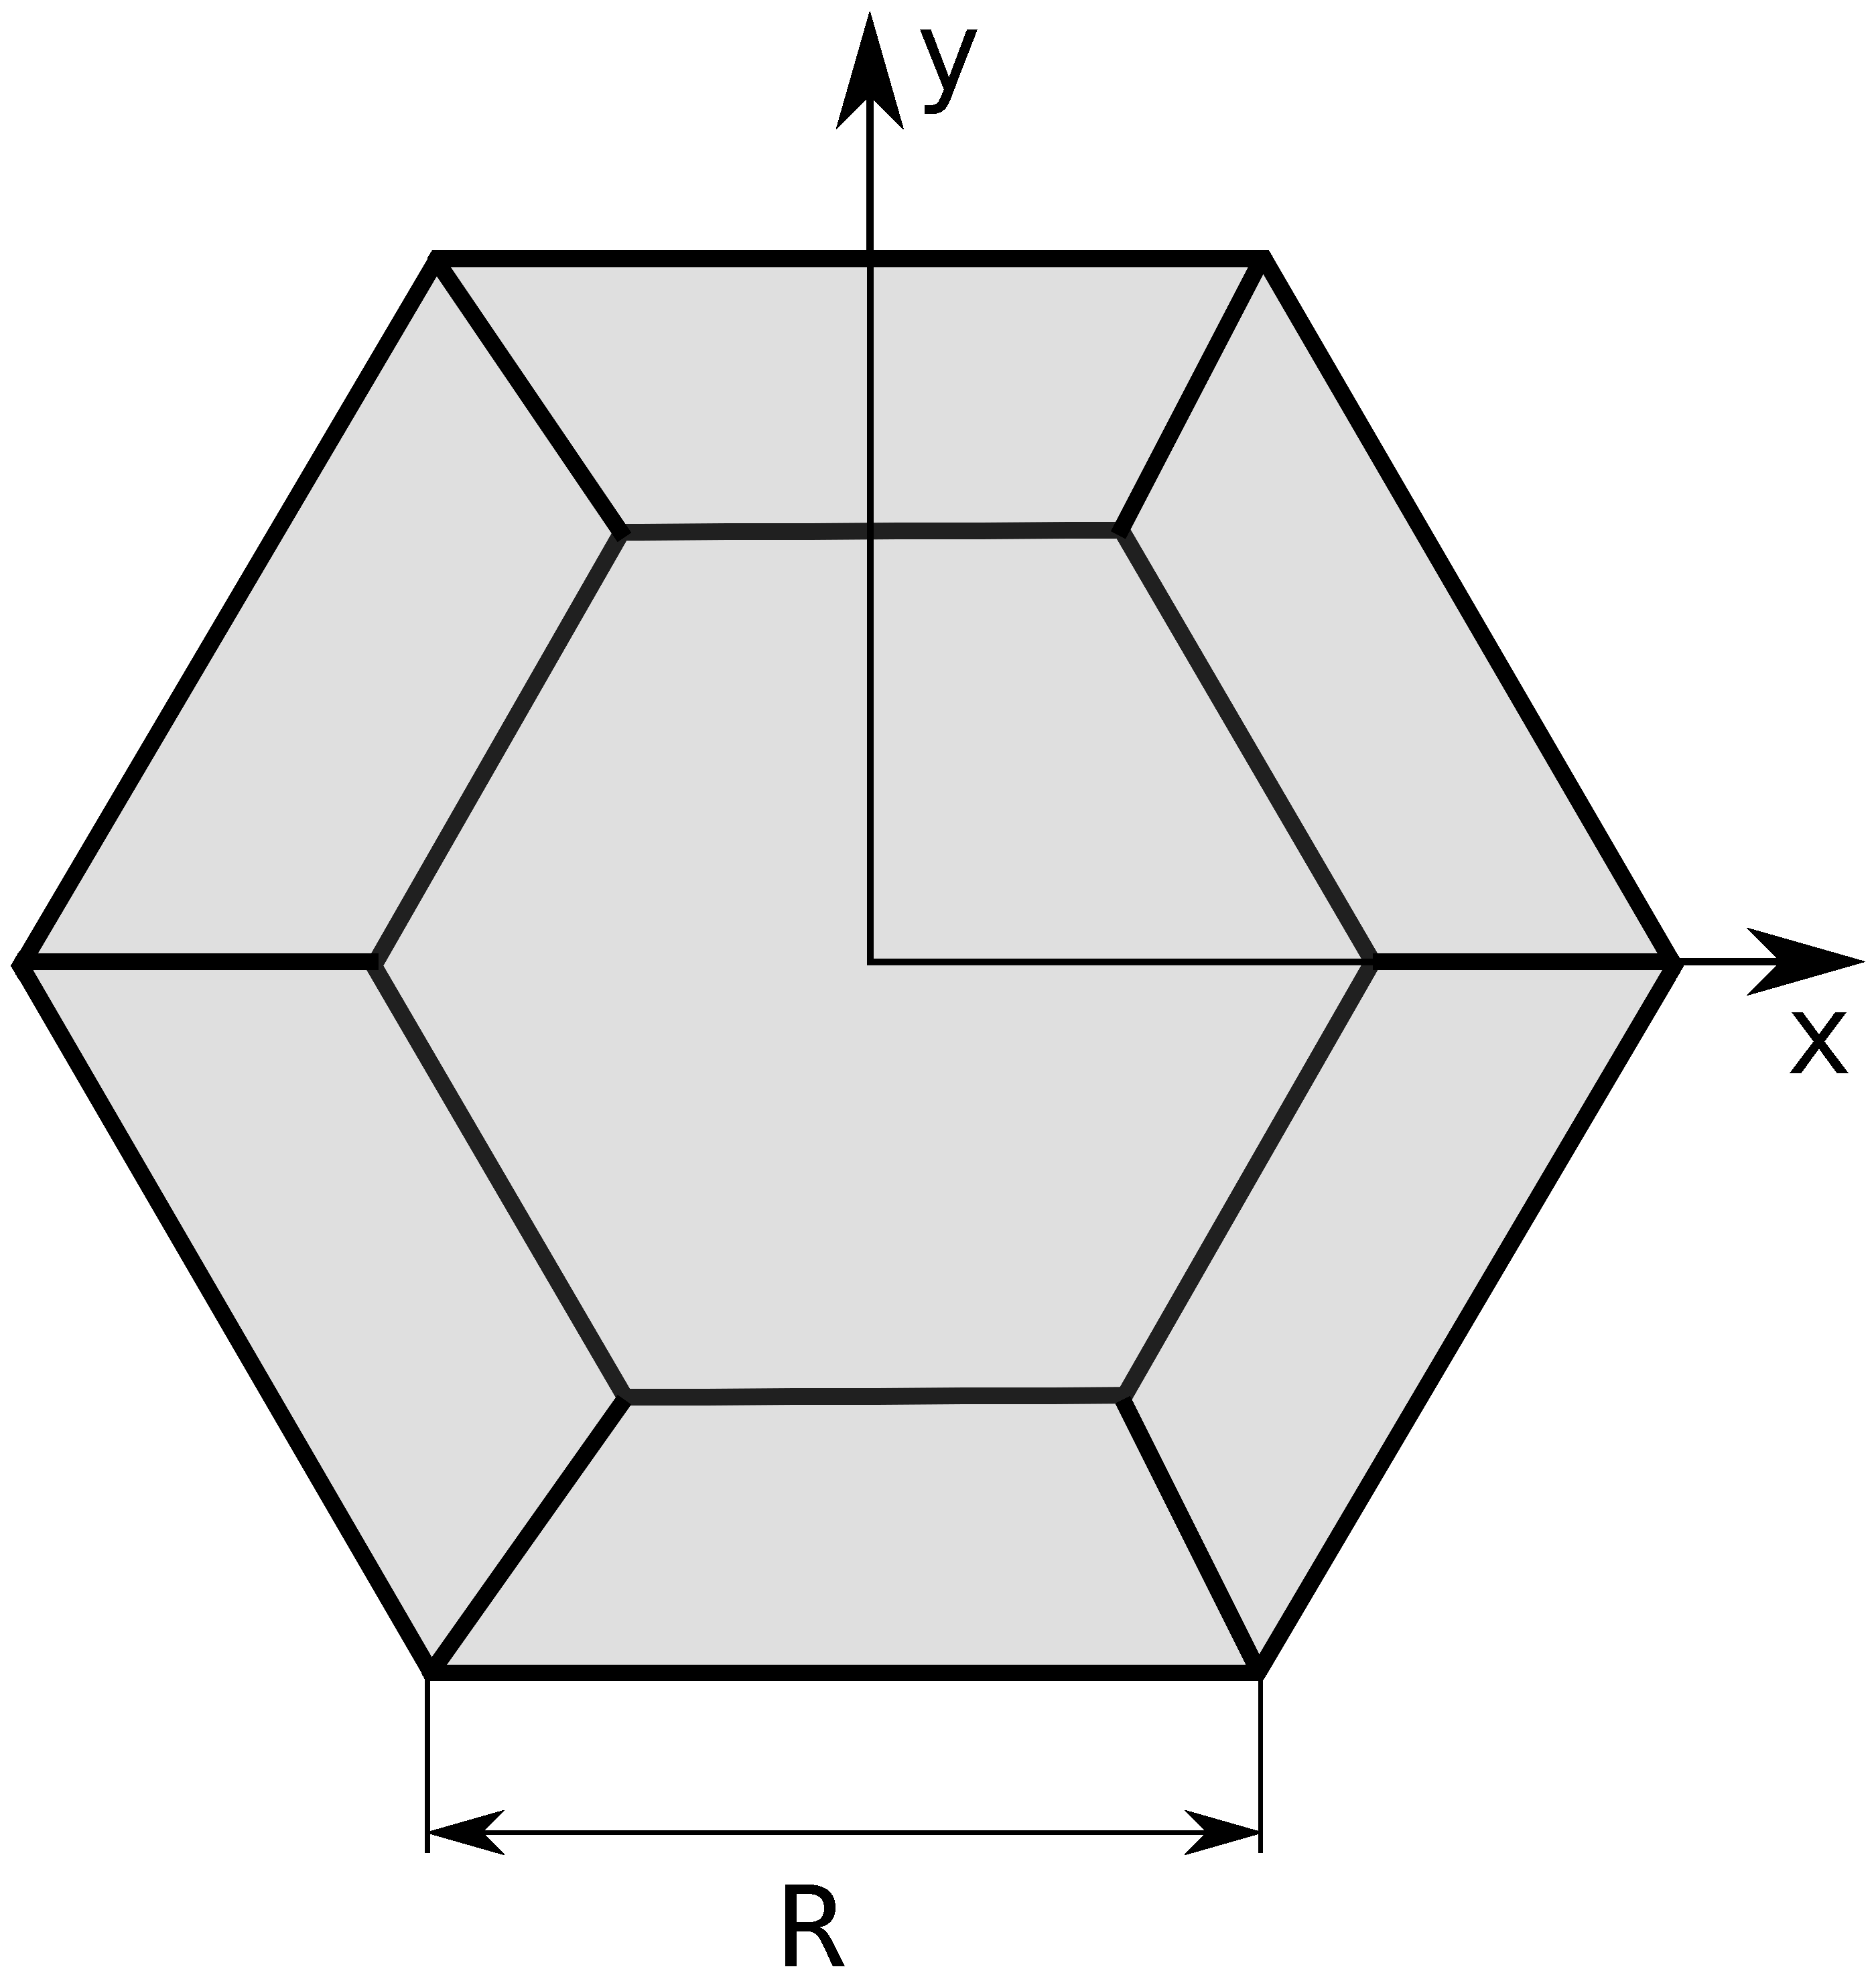
\includegraphics[width=5cm]{fig/cuts/Cone62dxy.eps}}
\hfill
\caption{Sketch of a Cone6.  The implementation of this shape uses angle
  $\alpha$, which is linked to $\beta$ via $\tan \alpha = \dfrac{2}{\sqrt{3}} \tan 
  \beta$. $\alpha$ is measured along one of the base lines and $\beta$
  at one of the base vertices.}
\label{fig:cone6}
\end{figure}

\FloatBarrier

\paragraph{Parameters}
\begin{itemize}
\item radius of the regular hexagonal base $R$,
\item height $H$,
\item angle $\alpha$ is considered between one of the side faces and
  the middle of a base length. 
\end{itemize}

\paragraph{Restrictions on the parameters:} 
$\dfrac{2H}{\sqrt{3}R}< \tan{\alpha}$.

\paragraph{Properties}
\begin{itemize}
\item volume $V = \dfrac{3}{4} \tan(\alpha) R^3 \left[
            1 - \left(1- \dfrac{2H}{ \tan(\alpha) R\sqrt{3}}\right)^3
            \right]$,
\item  particle surface seen from above $S =\dfrac{3\sqrt{3}R^2}{2}$.
\end{itemize}

\paragraph{Expression of the form factor}\mbox{}\\
The
calculation can be derived from ``Prism6'' (\SecRef{Prism6}) by
considering a side length varying with the vertical position:

\begin{align*}
F(\mathbf{q}, R, H, \alpha) = \frac{4\sqrt{3}}{3q_y ^2 - q_x^2}\int_0 ^H &\exp(iq_z z)
\Big[\frac{3}{4}R_z^2q_y^2 \sinc\left(\frac{q_xR_z}{2}\right)\sinc\left(\frac{\sqrt{3}q_y
R_z}{2}\right)\\
&+\cos(q_xR_z)-\cos\left(\frac{\sqrt{3}q_y R_z}{2}\right)\cos\left(\frac{q_xR_z}{2}\right) \Big]dz
\end{align*}
with $R_z=R-\dfrac{2z}{\sqrt{3}\tan(\alpha)}$ and $\sinc(x)=\sin(x)/x$.

\paragraph{Syntax} \Code{FormFactorCone6(radius,height, alpha)} 

\paragraph{Example}\mbox{}\\
Figure~\ref{fig:FFCone6Ex} shows the normalized intensity
$|F|^2/V^2$, computed with $R=10$~nm, $H=13$~nm, and
$\alpha=60^{\circ}$.

\begin{figure}[ht]
\begin{center}
\includegraphics[angle=-90,width=\textwidth]{fig/ff/figffcone6.pdf}
\end{center}
\caption{Normalized intensity for the form factor of a Cone6 plotted against ($q_y$, $q_z$) and ($q_x$, $q_y$) and computed with \Code{FormFactorCone6(10.*nanometer,13.*nanometer, 60.*degree)}.}
\label{fig:FFCone6Ex}
\end{figure}

\paragraph{References}
Agrees with \lq\lq Cone6\rq\rq ~form factor of \IsGISAXS~\cite{Laz02} ???

%-------------------------------------------------------------------------------
\newpage
\subsubsection{Pyramid (square-based)}\SecLabel{Pyramid}
  \index{Pyramid (form factor)!square base}
  \index{Truncated pyramid (form factor)!square base}
  \index{FormFactorPyramid@\Code{FormFactorPyramid}}
%-------------------------------------------------------------------------------

\paragraph{Real-space geometry}\mbox{}\\
This shape is a  truncated pyramid with a square base as shown in fig.~\ref{fig:pyramid}.

\begin{figure}[ht]
\hfill
\subfigure[Side view]{\includegraphics[width=5cm]{fig/cuts/Pyramid2dxz.eps}}
\hfill
\subfigure[Top view]{\includegraphics[width=5cm]{fig/cuts/Pyramid2dxy.eps}}
\hfill
\caption{Sketch of a Pyramid}
\label{fig:pyramid}
\end{figure}

\FloatBarrier

\paragraph{Parameters}
\begin{itemize}
\item length of one side of the square base $L$,  
\item height $H$,
\item  $\alpha$ is the angle between the base and the
  side faces, taken in the middle of the base lines.
\end{itemize}

\paragraph{Restrictions on the parameters:}  $\dfrac{2H}{L} < \tan(\alpha)$.

\paragraph{Properties}
\begin{itemize}
\item  volume $V = \dfrac{1}{6} \tan(\alpha) L^3\left[ 1
             - \left(1 - \dfrac{2H}{\tan(\alpha)L}\right)^3 \right],$
\item particle surface seen from above $S = L^2$.
\end{itemize}

\paragraph{Expression of the form factor}
\begin{align*}
&F(\mathbf{q},L, H, \alpha) =
\frac{H}{q_x q_y} \times \nonumber \\ &\left\{ K_1 \cos\left[
  (q_x-q_y)\frac{L}{2} \right] + K_2 \sin\left[ (q_x-q_y)\frac{L}{2} \right]
- K_3 \cos\left[ (q_x+q_y) \frac{L}{2} \right] - K_4 \sin\left[ (q_x+q_y)\frac{L}{2} \right]\right\},
\end{align*}
with $\sinc(x)=\sin(x)/x$,
\begin{align*}
       q_1 &=\frac{1}{2}\Big[\frac{q_x-q_y}{\tan(\alpha)} + q_z\Big],\quad       q_2 =\frac{1}{2}\Big[\frac{q_x-q_y}{\tan(\alpha)} - q_z\Big]\\
        q_3 &=\frac{1}{2}\Big[\frac{q_x+q_y}{\tan(\alpha)} + q_z\Big],\quad       q_4 =\frac{1}{2}\Big[\frac{q_x+q_y}{\tan(\alpha)} - q_z\Big]\\
        K_1 &= \sinc(q_1 H)\exp(i q_1 H)  + \sinc(q_2 H) \exp(-i q_2 H)\\
        K_2 &= -i \sinc(q_1 H) \exp(i q_1 H) +i \sinc(q_2 H) \exp(-i q_2 H)\\
        K_3 &= \sinc(q_3 H) \exp(i q_3 H)    + \sinc(q_4 H) \exp(-i q_4 H)\\
        K_4 &= -i \sinc(q_3 H) \exp(i q_3 H) + i \sinc(q_4 H) \exp(-i q_4 H) 
   \end{align*}

\paragraph{Syntax}  \Code{FormFactorPyramid(length, height, alpha)}

\paragraph{Examples}
Figure~\ref{fig:FFPyramidEx} shows the normalized intensity
$|F|^2/V^2$, computed with $L=18$~nm, $H=13$~nm and
$\alpha=60^{\circ}$.

\begin{figure}[ht]
\begin{center}
\includegraphics[angle=-90,width=\textwidth]{fig/ff/figffpyramid.pdf}
\end{center}
\caption{Normalized intensity for the form factor of a
  pyramid plotted against ($q_y$, $q_z$) and  
  ($q_x$, $q_y$) and computed with  \Code{FormFactorPyramid(18.*nanometer, 13.*nanometer, 60.*degree)}.}
\label{fig:FFPyramidEx}
\end{figure}

\paragraph{References}
Agrees with \lq\lq Pyramid\rq\rq ~form factor of \IsGISAXS~\cite{Laz02},
except for different parametrization $L=2R_{\rm{\Code{IsGISXAXS}}}$.
[and sign problem??]

%-------------------------------------------------------------------------------
\newpage
\subsubsection{AnisoPyramid (rectangle-based)} \SecLabel{AnisoPyramid} 
  \index{Anisotropic pyramid (form factor)}
  \index{Pyramid (form factor)!rectangular base (AnisoPyramid)}
  \index{Truncated pyramid (form factor)!rectangular base (AnisoPyramid)}
  \index{FormFactorAnisoPyramid@\Code{FormFactorAnisoPyramid}}
%-------------------------------------------------------------------------------

\paragraph{Real-space geometry}\mbox{}\\
This shape is a truncated right pyramid with a rectangular base as
shown in fig.~\ref{fig:anisopyramid}.

\begin{figure}[ht]
\hfill
\subfigure[Side view]{\includegraphics[width=5cm]{fig/cuts/AnisoPyramid2dxz.eps}}
\hfill
\subfigure[Top view]{\includegraphics[width=5cm]{fig/cuts/AnisoPyramid2dxy.eps}}
\hfill
\caption{Sketch of an Anisotropic Pyramid.}
\label{fig:anisopyramid}
\end{figure}

\FloatBarrier

\paragraph{Parameters}
\begin{itemize}
\item full length of the base $L$,
\item full width of the base $W$,
\item height $H$,
\item $\alpha$ is the angle between the base and the
  side faces, taken in the middle of the base lines.
\end{itemize}

\paragraph{Restrictions on the parameters:} $\dfrac{2H}{L}< \tan(\alpha)$ and $\dfrac{2H}{W}< \tan(\alpha)$.

\paragraph{Properties}
\begin{itemize}
\item volume $V= H \Big[LW - \dfrac{(L + W)H}{\tan(\alpha)}
   + \dfrac{4}{3} \dfrac{H^2}{\tan^2(\alpha)}\Big]$,
\item particle surface seen from above $S = LW$.
\end{itemize}

\paragraph{Expression of the form factor}
\begin{align*}
&F(\mathbf{q}, L, W, H, \alpha)=
\frac{H}{q_xq_y} \times \\
&\Big\{
K_1\cos\Big(q_x \frac{L}{2} -q_y \frac{W}{2}\Big)+  K_2 \sin \Big (q_x
\frac{L}{2}- q_y \frac{W}{2}\Big) - K_3 \cos \Big (q_x \frac{L}{2} +q_y \frac{W}{2}\Big)-
K_4 \sin \Big (q_x \frac{L}{2} + q_y \frac{W}{2}\Big)
\Big\},
\end{align*}
with $\sinc(x)=\sin(x)/x$,
\begin{align*}
K_1 &= \exp(-i q_2 H) \sinc(q_2 H) + \exp(iq_1 H) \sinc(q_1 H) \\
K_2 &= i \exp(-iq_2 H) \sinc(q_2 H) -i \exp(iq_1 H) \sinc(q_1 H) \\
K_3 &= \exp(-iq_4 H) \sinc(q_4 H) + \exp(iq_3 H) \sinc(q_3 H) \\
K_4 &= i \exp(i q_4 H) \sinc(q_4 H) -i \exp(iq_3 H) \sinc(q_3 H)\\
q_1 &= \frac{1}{2}\left[\frac{q_x -q_y}{\tan \alpha} +q_z \right],\quad q_2 = \frac{1}{2}\left[\frac{q_x -q_y}{\tan \alpha} -q_z \right]\\
q_3 &= \frac{1}{2}\left[\frac{q_x +q_y}{\tan \alpha} +q_z \right] , \quad q_4 = \frac{1}{2}\left[\frac{q_x +q_y}{\tan \alpha} -q_z \right]
\end{align*}

\paragraph{Syntax} \Code{FormFactorAnisoPyramid(length, width, height, alpha)}

\paragraph{Example}\mbox{}\\
Figure~\ref{fig:FFAnisoPyramidEx} shows the normalized intensity
$|F|^2/V^2$, computed with $L=20$~nm, $W=16$~nm, $H=13$~nm, and
$\alpha=60^{\circ}$.

\begin{figure}[ht]
\begin{center}
\includegraphics[angle=-90,width=\textwidth]{fig/ff/figffanisopyramid.pdf}
\end{center}
\caption{Normalized intensity for the form factor of an anisotropic
  pyramid $|F|^2/V^2$, plotted against ($q_y$, $q_z$) and  ($q_x$, $q_y$) and computed with \Code{FormFactorAnisoPyramid(20.*nanometer, 16.*nanometer, 60.*degree)}.}
\label{fig:FFAnisoPyramidEx}
\end{figure}

\paragraph{References}
Agrees with \lq\lq AnisoPyramid\rq\rq ~form factor of \IsGISAXS~\cite{Laz02},
except for different parametrization. ???

%\subsubsection{References}
%Like in \Code{IsGISAXS}, the base angle $\alpha$ is the same for both unequal
%side. This means that a full anisotropic pyramid is not a limit case. \\
%But \BornAgain\ uses a different convention of the parameters relative
%to the base. We input the full length and width instead of half values.
%Condition on the parameters: 
%Should not it be: H/R < tan(alpha) and  H/W < tan(alpha) instead of H/R < tan(alpha) and  
%W/R < tan(alpha) where H is the height and R, W the side-lengths of the rectangular base?

%-------------------------------------------------------------------------------
\newpage
\subsubsection{Cuboctahedron} \SecLabel{Cuboctahedron}
  \index{Cuboctahedron (form factor)}
  \index{FormFactorCuboctahedron@\Code{FormFactorCuboctahedron}}
%-------------------------------------------------------------------------------

\paragraph{Real-space geometry}\mbox{}\\
It is a combination of two pyramids with square bases, as shown in fig.~\ref{fig:cuboctahedron}: the bottom one
is upside down with an height $H$ and the top one has the opposite
orientation (the standard one) and an height $r_H \times H$.

\begin{figure}[ht]
\hfill
\subfigure[Side view]{\includegraphics[width=5cm]{fig/cuts/Cuboctahedron2dxz.eps}}
\hfill
\subfigure[Top view]{\includegraphics[width=5cm]{fig/cuts/Cuboctahedron2dxy.eps}}
\hfill
\caption{Sketch of a Cuboctahedron.}
\label{fig:cuboctahedron}
\end{figure}

\FloatBarrier

\paragraph{Parameters}
\begin{itemize}
\item length of the shared square base $L$,
\item height $H$,
\item height\_ratio $r_H$,
\item $\alpha$ is the angle between the base and the
  side faces, taken in the middle of the base lines (see
  fig.~\ref{fig:pyramid} in \SecRef{Pyramid}).
\end{itemize}

\paragraph{Restrictions on the parameters:} $\dfrac{2H}{L}< \tan(\alpha)$ and $\dfrac{2r_HH}{L}< \tan(\alpha)$.

\paragraph{Properties}
\begin{itemize}
\item volume $ V= \dfrac{1}{6} \tan(\alpha)L^3 \Big[ 2
         - \Big(1 - \dfrac{2H }{L\tan(\alpha)} \Big)^3
           - \Big(1 - \dfrac{2 r_H
             H}{L\tan(\alpha) }\Big)^3\Big]$,
\item particle surface seen from above $S =L^2$.
\end{itemize}

\paragraph{Expression of the form factor}
\begin{equation*}
F(\mathbf{q}, L, H, r_H, \alpha)=\exp(iq_z
H)\Big[F_{\rm{Pyramid}}(q_x,q_y, q_z, L, r_H H,
\alpha)+F_{\rm{Pyramid}}(q_x, q_y, -q_z, L, H, \alpha))\Big]
\end{equation*}

\paragraph{Syntax} \Code{FormFactorCuboctahedron(length, height, height\_ratio,
  alpha)}

\paragraph{Example}\mbox{}\\
Figure~\ref{fig:FFcuboctahEx} shows the normalized intensity $|F|^2/V^2$, computed with $L=20$~nm, $H=13$~nm, $r_H=0.7$, and $\alpha=60^{\circ}$.
\begin{figure}[ht]
\begin{center}
\includegraphics[angle=-90,width=\textwidth]{fig/ff/figffcuboctah.pdf}
\end{center}
\caption{Normalized intensity for the form factor of a cuboctahedron plotted against ($q_y$, $q_z$) and  ($q_x$, $q_y$) and computed with \Code{FormFactorCuboctahedron(20.*nanometer, 13.*nanometer, 0.7, 60.*degree)}.}
\label{fig:FFcuboctahEx}
\end{figure}

\paragraph{References}
Agrees with \lq\lq \rq\rq Cuboctahedron~form factor of \IsGISAXS~\cite{Laz02},
except for different parametrization $L=2R_{\rm{\Code{IsGISAXS}}}$.

%-------------------------------------------------------------------------------
\newpage
\subsubsection{Cylinder} \SecLabel{Cylinder}
  \index{Cylinder (form factor)}
  \index{FormFactorCylinder@\Code{FormFactorCylinder}}
%-------------------------------------------------------------------------------
 
\paragraph{Real-space geometry}\mbox{}\\
This shape is a right circular cylinder (see fig.~\ref{fig:cylinder}).

\begin{figure}[ht]
\hfill
\subfigure[Side view]{\includegraphics[width=5cm]{fig/cuts/Cylinder2dxz.eps}}
\hfill
\subfigure[Top view]{\includegraphics[width=5cm]{fig/cuts/Cylinder2dxy.eps}}
\hfill
\caption{Sketch of a Cylinder.}
\label{fig:cylinder}
\end{figure}

\paragraph{Parameters}
\begin{itemize}
\item radius of the circular base $R$, 
\item height $H$.
\end{itemize}

\paragraph{Properties}
\begin{itemize}
\item volume $V = \pi R^2 H$,
\item particle surface seen from above $S=\pi R^2$.

\end{itemize}

\paragraph{Expression of the form factor}
  \begin{equation*}
F(\mathbf{q},R, H)=  2\pi
 R^2 H  \sinc\left(q_ z \frac{H}{2}\right) \exp\left(i q_ z \frac{H}{2}\right) \frac{J_1(q_{\parallel} R )}{q_{\parallel} R },
 \end{equation*}
with $q_{\parallel}=\sqrt{q_x^2+q_y^2}$ and $J_1(x)$ is the first order
Bessel function of the first kind \cite{AbSt64}.

\paragraph{Syntax} \Code{FormFactorCylinder(radius, height)}

\newpage

\paragraph{Example}\mbox{}\\
Figure~\ref{fig:FFcylinderEx} shows the normalized intensity
$|F|^2/V^2$, computed with $R=8$~nm and \mbox{$H=16$~nm.}
\begin{figure}[ht]
\begin{center}
\includegraphics[angle=-90,width=\textwidth]{fig/ff/figffcylinder.pdf}
\end{center}
\caption{Normalized intensity for the form factor of a cylinder plotted against ($q_y$, $q_z$) and  ($q_x$, $q_y$.) It
has been  computed with \Code{FormFactorCylinder(8.*nanometer, 16.*nanometer)}.}
\label{fig:FFcylinderEx}
\end{figure}

\paragraph{References}
Agrees with \lq\lq \rq\rq Cylinder~form factor of \IsGISAXS~\cite{Laz02}.

%-------------------------------------------------------------------------------
\newpage
\subsubsection{EllipsoidalCylinder} \SecLabel{EllipsoidalCylinder} 
  \index{Ellipsoidal cylinder (form factor)}
  \index{Cylinder (form factor)!ellipsoidal}
  \index{FormFactorEllipsoidalCylinder@\Code{FormFactorEllipsoidalCylinder}}
%-------------------------------------------------------------------------------

\paragraph{Real-space geometry}\mbox{}\\
This is a cylinder whose cross section is an ellipse.

\begin{figure}[ht]
\hfill
\subfigure[Side view]{\includegraphics[width=5cm]{fig/cuts/EllipsoidalCylinder2dxz.eps}}
\hfill
\subfigure[Top view]{\includegraphics[width=5cm]{fig/cuts/EllipsoidalCylinder2dxy.eps}}
\hfill
\caption{Sketch of an Ellipsoidal Cylinder.}
\label{fig:ellipscylinder}
\end{figure}

\paragraph{Parameters}
\begin{itemize}
\item $r_a$ = half length of the ellipse main axis parallel to $x$,
\item$r_b$ = half length of the ellipse main axis parallel to $y$, 
\item height $H$.
\end{itemize}

\paragraph{Properties}
\begin{itemize}
\item volume $V = \pi r_a r_bH$,
\item particle surface seen from above $S = r_a r_b$.
\end{itemize}

\paragraph{Expression of the form factor}
The total form factor is given by 
\begin{equation*}
F(\mathbf{q},R,W,H) = 2\pi r_a r_b H \exp\left(i\frac{q_z
  H}{2}\right)\sinc\left(\frac{q_z H}{2}\right) \frac{J_1(\gamma)}{\gamma},
\end{equation*}
with $\gamma=\sqrt{(q_x r_a)^2+(q_y r_b)^2}$ and $J_1(x)$ is the first order
Bessel function of the first kind \cite{AbSt64}.

\paragraph{Syntax} \Code{FormFactorEllipsoidalCylinder($r_a$, $r_b$, height)}

\newpage


\paragraph{Example}\mbox{}\\
Figure~\ref{fig:FFellipscylinderEx} shows the normalized intensity
$|F|^2/V^2$, computed with $r_a=13$~nm, $r_b=8$~nm, and $H=16$~nm.
\begin{figure}[ht]
\begin{center}
\includegraphics[angle=-90,width=\textwidth]{fig/ff/figffellipscylinder.pdf}
\end{center}
\caption{Normalized intensity for the form factor of an ellipsoidal
  cylinder plotted against ($q_y$, $q_z$) and ($q_x$,
  $q_y$) and computed with \Code{FormFactorEllipsoidalCylinder(8.*nanometer, 13.*nanometer, 16*nanometer)}.}
\label{fig:FFellipscylinderEx}
\end{figure}

\paragraph{References}
Agrees with \lq\lq Ellipsoid \rq\rq ~form factor of \IsGISAXS~\cite{Laz02}.

%-------------------------------------------------------------------------------
\newpage
\subsubsection{Cone (circular)} \SecLabel{Cone} 
  \index{Cone (form factor)!circular}
  \index{Truncated cone (form factor)}
  \index{FormFactorCone@\Code{FormFactorCone}}
%-------------------------------------------------------------------------------

\paragraph{Real-space geometry}
This shape is a truncated cone as shown in fig.~\ref{fig:cone}. 

\begin{figure}[ht]
\hfill
\subfigure[Side view]{\includegraphics[width=5cm]{fig/cuts/Cone2dxz.eps}}
\hfill
\subfigure[Top view]{\includegraphics[width=5cm]{fig/cuts/Cone2dxy.eps}}
\hfill
\caption{Sketch of a Cone.}
\label{fig:cone}
\end{figure}

\paragraph{Parameters}
\begin{itemize}
\item radius $R$,
\item height $H$,
\item $\alpha$ is the angle between the side and the circular base.
\end{itemize}

\paragraph{Restrictions on the parameters:} $\dfrac{H}{R}< \tan(\alpha)$.

\paragraph{Properties}
\begin{itemize}
\item volume $V = \dfrac{\pi}{3} \tan(\alpha) R^3 \left[ 
            1 - \left(1- \dfrac{H}{\tan(\alpha)R}\right)^3\right]$,
\item  particle surface seen from above $S=\pi R^2$.
\end{itemize}

\paragraph{Expression of the form factor}
\begin{equation*}
F(\mathbf{q}, R, H, \alpha) = \int_0 ^H 2\pi R_z^2
\frac{J_1(q_{\parallel}R_z)}{q_{\parallel} R_z}\exp(iq_z z)dz,
\end{equation*}
with $R_z =R-\dfrac{z}{\tan \alpha}$, $\mathbf{q}_{\parallel}=\sqrt{q_x^2+ q_y^2}$ and $J_1(x)$ is the first order
Bessel function of the first kind \cite{AbSt64}.

\paragraph{Syntax}  \Code{FormFactorCone(radius, height, alpha)}. 

\paragraph{Example}\mbox{}\\
Figure~\ref{fig:FFConeEx} shows the normalized intensity
$|F|^2/V^2$, computed with $R=10$~nm, $H=13$~nm, and $\alpha=60^{\circ}$.
\begin{figure}[ht]
\begin{center}
\includegraphics[angle=-90,width=\textwidth]{fig/ff/figffcone.pdf}
\end{center}
\caption{Normalized intensity for the form factor of a Cone plotted against ($q_y$, $q_z$) and ($q_x$, $q_y$.) It
  has been  computed with \Code{FormFactorCone(10.*nanometer,13.*nanometer, 60.*degree)}.}
\label{fig:FFConeEx}
\end{figure}

\paragraph{References}
Agrees with \lq\lq Cone \rq\rq ~form factor of \IsGISAXS~\cite{Laz02}.

%-------------------------------------------------------------------------------
\newpage
\subsubsection{FullSphere} \SecLabel{FullSphere}
  \index{Full sphere (form factor)}
  \index{Sphere (form factor)}
  \index{FormFactorFullSphere@\Code{FormFactorFullSphere}}
%-------------------------------------------------------------------------------

\paragraph{Real-space geometry}\mbox{}\\
The full sphere is parametrized by its radius $R$. 

\begin{figure}[ht]
\hfill
\subfigure[Side view]{\includegraphics[width=5cm]{fig/cuts/FullSphere2dxz.eps}}
\hfill
\subfigure[Top view]{\includegraphics[width=5cm]{fig/cuts/FullSphere2dxy.eps}}
\hfill
\caption{Sketch of a Full Sphere.}
\label{fig:fullsphere}
\end{figure}

\FloatBarrier

\paragraph{Parameters} radius $R$.

\paragraph{Properties}
\begin{itemize}
\item volume $V = \dfrac{4\pi}{3}R^3$,
\item particle surface seen from above $S= \pi R^2$.
%\item radius of gyration
\end{itemize}

\paragraph{Expression of the form factor}
\begin{equation*}
F(\mathbf{q},R) = 4\pi R^3 \exp(iq_z R)\frac{\sin(q R) - q R \cos(q R)}{(qR)^3},
\end{equation*}
where $q=\sqrt{q_x^2 + q_y^2 + q_z^2}$.

\paragraph{Syntax} \Code{FormFactorFullSphere(radius)}

\newpage

\paragraph{Example}\mbox{}\\
Figure~\ref{fig:FFfSphereEx} shows the normalized intensity $|F|^2/V^2$, computed with $R=8$~nm.
\begin{figure}[ht]
\begin{center}
\includegraphics[angle=-90,width=\textwidth]{fig/ff/figfffsphere.pdf}
\end{center}
\caption{Normalized intensity for the
  form factor of a Full Sphere plotted against ($q_y$, $q_z$) and ($q_x$, $q_y$) and computed with \Code{FormFactorFullSphere(8.*nanometer)}.}
\label{fig:FFfSphereEx}
\end{figure}

\paragraph{References}
Agrees with \lq\lq ?? \rq\rq ~form factor of \IsGISAXS~\cite{Laz02}.


%-------------------------------------------------------------------------------
\newpage
\subsubsection{TruncatedSphere}\SecLabel{Sphere}
  \index{Sphere (form factor)!truncated}
  \index{Truncated sphere (form factor)}
  \index{FormFactorTruncatedSphere@\Code{FormFactorTruncatedSphere}}
%-------------------------------------------------------------------------------
  
\paragraph{Real-space geometry}\mbox{}\\
This shape is a spherical dome, \textit{i.e.} a portion of a sphere cut off by a plane (perpendicular
to $z$-axis) as shown in fig.~\ref{fig:sphere}.

\begin{figure}[ht]
\hfill
\subfigure[Side view]{\includegraphics[width=5cm]{fig/cuts/Sphere2dxz.eps}}
\hfill
\subfigure[Top view]{\includegraphics[width=5cm]{fig/cuts/Sphere2dxy.eps}}
\hfill
\caption{Sketch of a Truncated Sphere.}
\label{fig:sphere}
\end{figure}
\FloatBarrier

\paragraph{Parameters}
\begin{itemize}
\item radius $R$,
\item height $H$.
\end{itemize}

\paragraph{Restrictions on the parameters:} $0 \leq H\leq 2R$.

\paragraph{Properties}
\begin{itemize}
\item volume $V=\pi R^3 \left[\dfrac{2}{3} + \dfrac{H-R}{R} - \dfrac{1}{3}\left(\dfrac{H-R}{R}\right)^3\right]$,
\item particle surface seen from above $S = \left\{\begin{array}{ll} \pi R^2, & H \geq R \\
         \pi\left(2RH-H^2\right), & H < R \end{array}\right. $.
%\item gyration radius along $z$ axis %$R_g = \left\{\begin{array}{ll}
%R, & H > R \\ \sqrt{2RH-H^2}, & H < R \end{array}\right. .$
\end{itemize}

\paragraph{Expression of the form factor}
\begin{equation*}  
F(\mathbf{q},R, H)= 2\pi \exp[i q_z (H-R)]\int_{R-H} ^{R} R_z^2 \frac{J_1(q_{\parallel} R_z) }{q_{\parallel} R_z} \exp(i q_z z) dz,
\end{equation*}
with $J_1(x)$ the first order
Bessel function of the first kind \cite{AbSt64}, $q_{\parallel} =
\sqrt{q_x^2+q_y^2}$, and $R_z = \sqrt{R^2-z^2}$

\paragraph{Syntax} \Code{FormFactorTruncatedSphere(radius, height)}

\paragraph{Example}\mbox{}\\
Figure~\ref{fig:SphereEx} shows the normalized intensity $|F|^2/V^2$, computed with $R=5$~nm and $H=7$~nm:
\begin{figure}[ht]
\begin{center}
\includegraphics[angle=-90,width=\textwidth]{fig/ff/figffsphere.pdf}
\end{center}
\caption{Normalized intensity for the form factor of a Truncated Sphere plotted against ($q_y$, $q_z$) and ($q_x$, $q_y$) and
  computed with \Code{FormFactorTruncatedSphere(5.*nanometer, 7.*nanometer)}.}
\label{fig:SphereEx}
\end{figure}

\paragraph{References}
Agrees with \lq\lq Sphere\rq\rq ~form factor of \IsGISAXS~\cite{Laz02}.

%-------------------------------------------------------------------------------
\newpage
\subsubsection{FullSpheroid} \SecLabel{FullSpheroid}
  \index{Full spheroid (form factor)}
  \index{Spheroid (form factor)}
  \index{FormFactorFullSpheroid@\Code{FormFactorFullSpheroid}}
%-------------------------------------------------------------------------------

\paragraph{Real-space geometry}\mbox{}\\
A full spheroid is generated by rotating an ellipse around the vertical
axis (see fig.~\ref{fig:fullspheroid}).

\begin{figure}[ht]
\hfill
\subfigure[Side view]{\includegraphics[width=5cm]{fig/cuts/FullSpheroid2dxz.eps}}
\hfill
\subfigure[Top view]{\includegraphics[width=5cm]{fig/cuts/FullSpheroid2dxy.eps}}
\hfill
\caption{Sketch of a Full Spheroid. }
\label{fig:fullspheroid}
\end{figure}

\FloatBarrier

\paragraph{Parameters}
\begin{itemize}
\item radius $R$,
\item height $H$.
\end{itemize}

\paragraph{Properties}
\begin{itemize}
\item volume $V =\dfrac{2}{3}R^2H$,
\item particle surface seen from above $S =\pi R^2$. 
\end{itemize}

\paragraph{Expression of the form factor}
\begin{equation*}
F(\mathbf{q}, R, H) = 4\pi \exp(i q_z H/2) \int_0 ^{H/2}R_z ^2
\frac{J_1(q_{\parallel}R_z)}{q_{\parallel}R_z} \cos(q_z z) dz,
\end{equation*}
with $J_1(x)$ the first order
Bessel function of the first kind \cite{AbSt64},
$R_z = R\sqrt{1-\frac{4z^2}{H^2}}$, $\gamma_z = \sqrt{(q_x R_z)^2+(q_y R_z)^2}$.


\paragraph{Syntax} \Code{FormFactorFullSpheroid(radius,height)}
\newpage

\paragraph{Example}\mbox{}\\
Figure~\ref{fig:FFfspheroidEx} shows the normalized intensity
$|F|^2/V^2$, computed with $R=10$~nm, and $H=13$~nm.
\begin{figure}[ht]
\begin{center}
\includegraphics[angle=-90,width=\textwidth]{fig/ff/figfffspheroid.pdf}
\end{center}
\caption{Normalized intensity for the form factor of a full spheroid plotted against ($q_y$, $q_z$) and ($q_x$, $q_y$) and
  computed with \Code{FormFactorFullSpheroid(10.*nanometer, 13.*nanometer)}.}
\label{fig:FFfspheroidEx}
\end{figure}

\paragraph{References}
Corrected version of the \lq\lq FullSpheroid \rq\rq ~form factor of \IsGISAXS~\cite{Laz02}.

%\subsubsection{References}
%The expression is identical to \Code{IsGISAXS} manual. In the code,
%the integration is over $[-H/2, H/2]$ with $\exp(iq_z z)$ instead of
%the cosine.
%In \Code{IsGISAXS}, factor 4 instead of 2 in the expression of the
%volume. In the code there is also a problem with an extra factor 2 in the function to integrate.

%-------------------------------------------------------------------------------
\newpage
\subsubsection{TruncatedSpheroid} \SecLabel{Spheroid}
  \index{Spheroid (form factor)!truncated}
  \index{Truncated spheroid (form factor)}
  \index{FormFactorTruncatedSpheroid@\Code{FormFactorTruncatedSpheroid}}
%-------------------------------------------------------------------------------

\paragraph{Real-space geometry}\mbox{}\\
This shape is a spheroidal dome: a portion of a full spheroid cut off
by a plane perpendicular to the $z$-axis.

\begin{figure}[ht]
\hfill
\subfigure[Side view]{\includegraphics[width=5cm]{fig/cuts/Spheroid2dxz.eps}}
\hfill
\subfigure[Top view]{\includegraphics[width=5cm]{fig/cuts/Spheroid2dxy.eps}}
\hfill
\caption{Sketch of a Truncated Spheroid.}
\label{fig:spheroid}
\end{figure}

\paragraph{Parameters}
\begin{itemize}
\item radius $R$,
\item height $H$,
\item height\_flattening coefficient in the perpendicular direction $f_p$.
\end{itemize}

\paragraph{Restrictions on the parameters:} $0< \dfrac{H}{R}< 2f_p$.

\paragraph{Properties}
\begin{itemize}
\item volume $V = \dfrac{\pi R H^2}{f_p}  \Big(1-\dfrac{H}{3f_p R}\Big)$,
\item particle surface seen from above $S = \left\{\begin{array}{ll} \pi R^2, & H \geq f_pR \\
         \pi\left(\dfrac{2RH}{f_p}-\dfrac{H^2}{f_p^2}\right), & H < R \end{array}\right.$.
\end{itemize}

\paragraph{Expression of the form factor}
\begin{equation*} 
F(\mathbf{q},R, H,f_p) =   2\pi \exp[iq_z(H-f_pR)] \int_{f_p R-H} ^{f_p R} R_z
        ^2\frac{J_1(q_{\parallel}R_z)}{q_{\parallel}R_z} \exp(i q_z z) dz
\end{equation*}
with $J_1(x)$ the first order
Bessel function of the first kind \cite{AbSt64}, $q_{\parallel}=\sqrt{q_x^2+q_y^2} $ and $R_z=\sqrt{R^2-z^2/f_p^2}$.

\paragraph{Syntax} \Code{FormFactorTruncatedSpheroid(radius, height, height\_flattening)}

\paragraph{Example}\mbox{}\\
Figure~\ref{fig:FFspheroidEx} shows the normalized intensity
$|F|^2/V^2$, computed with $R=7.5$~nm, $H=9$~nm and $f_p=1.2$.

\begin{figure}[ht]
\begin{center}
\includegraphics[angle=-90,width=\textwidth]{fig/ff/figffspheroid.pdf}
\end{center}
\caption{Normalized intensity for the form factor of a Truncated Spheroid plotted against ($q_z$, $q_y$) and ($q_x$, $q_y$) and
  computed with \Code{FormFactorTruncatedSpheroid(7.5*nanometer, 9.*nanometer, 1.2)}.}
\label{fig:FFspheroidEx}
\end{figure}

\paragraph{References}
Agrees with \lq\lq TruncatedSpheroid \rq\rq ~form factor
of \IsGISAXS~\cite{Laz02}.
% Note an erroneous factor~2 in the expression of the volume
% in the \Code{IsGISAXS} manual.


%-------------------------------------------------------------------------------
\newpage
\subsubsection{HemiEllipsoid} \SecLabel{HemiEllipsoid}  
  \index{Hemi ellipsoid (form factor)}
  \index{Ellipsoid (form factor)!truncated}
  \index{Truncated ellipsoid (form factor)}
  \index{FormFactorHemiEllipsoid@\Code{FormFactorHemiEllipsoid}}
%-------------------------------------------------------------------------------

\paragraph{Real-space geometry}\mbox{}\\
This shape is a truncated ellipsoid as shown in fig.~\ref{fig:hemiellipsoid}.

\begin{figure}[ht]
\hfill
\subfigure[Side view]{\includegraphics[width=5cm]{fig/cuts/HemiEllipsoid2dxz.eps}}
\hfill
\subfigure[Top view]{\includegraphics[width=5cm]{fig/cuts/HemiEllipsoid2dxy.eps}}
\hfill
\caption{Sketch of an Hemi-ellipsoid.}
\label{fig:hemiellipsoid}
\end{figure}

\paragraph{Parameters}
\begin{itemize}
\item $r_a$ = half length of the ellipse main axis parallel to $x$,
\item$r_b$ = half length of the ellipse main axis parallel to $y$, 
\item $H$ = height (half length of the vertical main axis of a full ellipsoid).
\end{itemize}

\paragraph{Properties}
\begin{itemize}
\item volume $V = \dfrac{2}{3}\pi r_a r_bH$,
\item particle surface seen from above $S =\pi r_a r_b$.
\end{itemize}

\paragraph{Expression of the form factor}
\begin{equation*}
F(\mathbf{q},r_a,r_b,H) = 2\pi \int_0 ^{H} r_{a,z} r_{b,z}
\frac{J_1(\gamma_z)}{\gamma_z}\exp(iq_z z)dz,
\end{equation*}
with $J_1(x)$ the first order
Bessel function of the first kind \cite{AbSt64}, $r_{a,z} = r_a \sqrt{1-\left(\dfrac{z}{H} \right)^2}$, ${r_{b,z} = r_b
\sqrt{1-\left(\dfrac{z}{H} \right)^2}}$ and $\gamma_z =\sqrt{(q_x r_{a,z})^2+(q_y r_{b,z})^2}$.

\paragraph{Syntax} \Code{FormFactorHemiEllipsoid($r_a$, $r_b$, height)}

\newpage

\paragraph{Example} \mbox{}\\
Figure~\ref{fig:FFhemiellipsEx} shows the normalized intensity
$|F|^2/V^2$, computed with $r_a=10$~nm, $r_b=6$~nm and $H=8$~nm.

\begin{figure}[ht]
\begin{center}
\includegraphics[angle=-90,width=\textwidth]{fig/ff/figffhemiellips.pdf}
\end{center}
\caption{Normalized intensity for the form factor of an Hemi-Ellipsoid plotted against ($q_y$, $q_z$) and  ($q_x$, $q_y$)
  computed with \Code{FormFactorHemiEllipsoid(10.*nanometer, 6.*nanometer, 8.*nanometer)}.}
\label{fig:FFhemiellipsEx}
\end{figure}

\paragraph{References}
Called \lq\lq Anisotropic hemi ellipsoid\rq\rq in \Code{ISGISAXS},
which seems to have a sign error in the $z$ dependence.


%-------------------------------------------------------------------------------
\newpage
\subsubsection{Ripple1 (sinusoidal)} \SecLabel{Ripple1}  
  \index{Ripple (form factor)!sinusoidal (Ripple1)}
  \index{Sinusoidal ripple (form factor)}
  \index{FormFactorRipple1@\Code{FormFactorRipple1}}
%-------------------------------------------------------------------------------

\paragraph{Real-space geometry}\mbox{}\\
This shape has a sinusoidal profile (see fig.~\ref{fig:ripple1}).

\begin{figure}[ht]
\hfill
\subfigure[Side view]{\includegraphics[width=5cm]{fig/cuts/Ripple12dyz.eps}}
\hfill
\subfigure[Top view]{\includegraphics[width=5cm]{fig/cuts/Ripple12dxy.eps}}
\hfill
\caption{Sketch of a Ripple1.}
\label{fig:ripple1}
\end{figure}

\paragraph{Parameters}
\begin{itemize}
\item length $L$, 
\item width $W$, 
\item height $H$. 
\end{itemize}

\paragraph{Properties}
\begin{itemize}
\item volume $V = \dfrac{L W H}{2} $,
\item particle surface seen from above $S = L W$.
\end{itemize}

\paragraph{Expression of the form factor}
\begin{align*}
F(\mathbf{q},L,W,H) &=L \cdot \frac{W}{\pi}\cdot \sinc\left(\frac{q_xL}{2}\right)\times \\ &\int_0^H{dz \arccos\left(\frac{2z}{H}-1\right)\sinc\left[\frac{q_yW}{2\pi}\arccos\left(\frac{2z}{H} - 1\right)\right]\exp\left(iq_zz\right)},
\end{align*}
where $\arccos$ is the  arc cosine (\textit{i.e.} the inverse
operation of cosine).

\paragraph{Syntax} \Code{FormFactorRipple1(length, width, height)}

\paragraph{Example}\mbox{}\\
Figure~\ref{fig:FFripple1Ex} shows the normalized intensity
$|F|^2/V^2$, computed with $L=27$~nm, $W=20$~nm and $H=14$~nm.

\begin{figure}[ht]
\begin{center}
\includegraphics[angle=-90,width=\textwidth]{fig/ff/figffripple1.pdf}
\end{center}
\caption{Normalized intensity for the form factor of a ripple1
  $|F|^2/V^2$, plotted against ($q_y$, $q_z$) and  ($q_x$, $q_y$)
  computed with \Code{FormFactorRipple1(27.*nanometer, 20.*nanometer, 14.*nanometer)}.}
\label{fig:FFripple1Ex}
\end{figure}


%-------------------------------------------------------------------------------
\newpage
\subsubsection{Ripple2 (saw-tooth)} \SecLabel{Ripple2}  
  \index{Ripple (form factor)!saw-tooth (Ripple2)}
  \index{Saw-tooth ripple (form factor)}
  \index{FormFactorRipple2@\Code{FormFactorRipple2}}
%-------------------------------------------------------------------------------

\paragraph{Real-space geometry}\mbox{}\\
This shape has an asymmetric saw-tooth profile.

\begin{figure}[ht]
\hfill
\subfigure[Side view]{\includegraphics[width=5cm]{fig/cuts/Ripple22dyz.eps}}
\hfill
\subfigure[Top view]{\includegraphics[width=5cm]{fig/cuts/Ripple22dxy.eps}}
\hfill
\caption{Sketch of a Ripple2.}
\label{fig:ripple2}
\end{figure}

\FloatBarrier

\paragraph{Parameters}
\begin{itemize}
\item length $L$, 
\item width $W$, 
\item height $H$,
\item asymmetry $d$. 
\end{itemize}

\paragraph{Restriction on the parameters:} $|d| < \frac{W}{2} $.

\paragraph{Properties}
\begin{itemize}
\item volume $V = \dfrac{L W H}{2}$,
\item particle surface seen from above $S = L W$.
\end{itemize}

\paragraph{Expression of the form factor}
\begin{align*}
F(\mathbf{q},L,W,H,d) &=L W
\sinc\left(\frac{q_xL}{2}\right)\times \\ &
\int_0^H 
\left(1-\frac{z}{H}\right)
 \sinc\left[\frac{q_y
    W}{2}\left(1-\frac{z}{H}\right)\right] 
\exp\left\{ i\left[q_zz -
    q_yd\left(1-\frac{z}{H}\right)\right]\right\} 
dz
\end{align*}

\paragraph{Syntax} \Code{FormFactorRipple2(length, width, height, asymmetry)}

\paragraph{Examples}
Figure~\ref{fig:FFripple2Ex} shows the normalized intensity
$|F|^2/V^2$, computed with $L=36$~nm, $W=25$~nm, $H=14$~nm, and $d=3$~nm.

\begin{figure}[ht]
\begin{center}
\includegraphics[angle=-90,width=\textwidth]{fig/ff/figffripple2.pdf}
\end{center}
\caption{Normalized intensity for the form factor of a ripple2 plotted against ($q_y$, $q_z$) and  ($q_x$, $q_y$)
  computed with \Code{FormFactorRipple2(36.*nanometer, 25.*nanometer, 14.*nanometer, 3.*nanometer)}.}
\label{fig:FFripple2Ex}
\end{figure}


%===============================================================================
\subsection{Core-shell particles} \label{subsec:CoreShell}
%===============================================================================
\index{Core-shell particles}

To generate a core-shell particle, the combination is performed using the following command:\\
\Code{ParticleCoreShell(shell\_particle, core\_particle, relative\_core\_position)},\\
where \Code{shell\_particle} and \Code{core\_particle} are the outer and inner parts of the core-shell particle, respectively. They refer to one of the form factors defined previously and to an associated material. For example, for the outer part,\\ \Code{shell\_particle=Particle(material\_shell, outer\_form\_factor)},\\ where \Code{material\_shell} is the material of the shell and \Code{outer\_form\_factor} is the shape of the outer part (cf. listing~\ref{lst:cshellsample}). \\ \Code{relative\_core\_position} defines the position of the inner shape with respect to the outer one; it is defined with respect to the center of the base of the particular form factor. An example in fig.~\ref{fig:coreshell} shows a core shell particle made of a box for the outer part and of a shifted pyramidal shape for the inner one.\\

Figure~\ref{fig:FFCoreShellBA} displays the output intensity scattered in the Born Approximation using the code listed in~\ref{lst:cshellsample} to generate the core-shell particle. 

\begin{figure}[ht]
\hfill
\subfigure[Side view]{\includegraphics[width=5cm]{fig/cuts/CoreShellParallPyrxz.eps}}
\hfill
\subfigure[Top view]{\includegraphics[width=5cm]{fig/cuts/CoreShellParallPyrxy.eps}}
\hfill
\caption{Example of a core-shell particle composed of a box with a pyramidal  inset. The relative core shell position is marked by the positions of the centers of the bases. }
\label{fig:coreshell}
\end{figure}

\newpage

\begin{lstlisting}[language=python,
  style=eclipseboxed,numbers=none,nolol,caption={\Code{Python} script
    to create a core-shell particle made of a box with a pyramidal shifted inset.},label={lst:cshellsample}]
    outer_ff = FormFactorBox(16.0*nanometer, 16.0*nanometer, 8.0*nanometer) 
    inner_ff = FormFactorPyramid(12.0*nanometer, 7.0*nanometer, 60.0*degree)
    shell_particle = Particle(m_shell, outer_ff)
    core_particle = Particle(m_core, inner_ff)
    core_position = kvector_t(1.5, 0.0, 0.0)

    particle = ParticleCoreShell(shell_particle, core_particle, core_position)
\end{lstlisting}

\begin{figure}[ht]
\begin{center}
\includegraphics[angle=-90,width=0.6\textwidth]{fig/gisasmap/CoreShellParallPyr.pdf}
\end{center}
\caption{Intensity map of a core-shell form factor in Born Approximation using  \Code{FormFactorBox(16*nanometer, 16*nanometer, 8*nanometer)} and \Code{FormFactorPyramid(12*nanometer, 7*nanometer, 60*degree)} for the outer and inner shells, respectively. The core particle is shifted by 1.5~nm in the $x$-direction with respect to the center of the outer shell. The sample used to generate the particle is listed in~\ref{lst:cshellsample}.  There is no substrate and no interference between the particles.}
\label{fig:FFCoreShellBA}
\end{figure}

%===============================================================================
\subsection{Rotation of particles}
%===============================================================================
\index{Rotation of particles}
\index{Orientation of particles}

The particles can be rotated in a different direction by using one of
the following transformations: \Code{CreateRotateX($\theta$),
  CreateRotateY($\theta$), CreateRotateZ($\theta$)}, where capital X, Y, Z mark rotations
around the associated axis and $\theta$ is the
angle of rotation from this axis. For example, the following \Code{Python}\ script shows how to rotate a pyramid by $45^{\circ}$ around
the $z$-axis:\\

\begin{lstlisting}[language=python, style=eclipseboxed,numbers=none,nolol]
    pyramid_ff = FormFactorPyramid(10*nanometer, 5*nanometer, deg2rad(54.73 ) )
    pyramid = Particle(m_particle, pyramid_ff)
    angle_around_z = 45.*degree
    transform = Transform3D.createRotateZ(angle_around_z)
    particle_layout = ParticleLayout()
    particle_layout.addParticle(pyramid, transform) 
\end{lstlisting}

%===============================================================================
\subsection{Polydispersity}
%===============================================================================

\index{Form factors|)}

%%%%%%%%%%%%%%%%%%%%%%%%%%%%%%%%%%%%%%%%%%%%%%%%%%%%%%%%%%%%%%%%%%%%%%%%%%%%%%%%
%%
%%   BornAgain User Manual
%%
%%   homepage:   http://www.bornagainproject.org
%%
%%   copyright:  Forschungszentrum Jülich GmbH 2015
%%
%%   license:    Creative Commons CC-BY-SA
%%
%%   authors:    Scientific Computing Group at MLZ Garching
%%               C. Durniak, M. Ganeva, G. Pospelov, W. Van Herck, J. Wuttke
%%
%%%%%%%%%%%%%%%%%%%%%%%%%%%%%%%%%%%%%%%%%%%%%%%%%%%%%%%%%%%%%%%%%%%%%%%%%%%%%%%%


\newpage
\chapter{Using the Python API}  \label{sec:Usage}


%%%%%%%%%%%%%%%%%%%%%%%%%%%%%%%%%%%%%%%%%%%%%%%%%%%%%%%%%%%%%%%%%%%%%%%%%%%%%%%%
\section{Running a simulation}
%%%%%%%%%%%%%%%%%%%%%%%%%%%%%%%%%%%%%%%%%%%%%%%%%%%%%%%%%%%%%%%%%%%%%%%%%%%%%%%%

A simulation of GISAS using \BornAgain\ consists of the following steps:
\begin{itemize}
\item define materials by specifying name and refractive index,
\item define layers by specifying thickness, roughness, material,
\item define embedded particles by specifying shape, size,
   constituting material, interference function,
\item embed the particles in layers, specifying density, position, orientation,
\item assemble a multilayered sample,
\item specify input beam and detector characteristics,
\item run the simulation,
\item save the simulated detector image.
\end{itemize}

\noindent
All these steps can be organized in either a Graphical User Interface (GUI) or by providing a Python script with the simulation description.
In the following, we describe how to write a
\Code{Python} script which runs a \BornAgain\ simulation. For tutorials about this programming language, the users are referred to \cite{Lut09}.


% More information about the general software architecture and \BornAgain\ internal design are given in \cref{sec:SoftwareArchitecture}.


%===============================================================================
\subsection{Units:}
%===============================================================================
\index{Units}

By default the angles are expressed in radians and the lengths are given in
nanometers.  But it is possible to use other units by
specifying them right after the value of the corresponding
parameter like, for example, \Code{20.0*micrometer}.


%===============================================================================
\subsection{A first example} \label{sec:Example1Python}
%===============================================================================

In this example, we simulate the scattering from a mixture of
cylindrical and prismatic nanoparticles without any interference
between them. These particles are placed in air, on top
of a substrate.\\ We are going to go through each step of the
simulation. The \Python\ code snippet specific to each stage will be given at
the beginning of the description.
More examples can be found at our project web site \url{http://www.bornagainproject.org/documentation/python_examples}

% But for the sake of completeness the full code is given
% in Appendix~\ref{PythonSimulationExampleScript}.

%-------------------------------------------------------------------------------
\subsubsection{Importing Python modules}
%-------------------------------------------------------------------------------

\begin{lstlisting}[language=python, style=eclipseboxed,name=ex1,nolol]
import numpy @\label{import_lib_beg}@
import matplotlib
import pylab @\label{import_lib_end}@
from bornagain import * @\label{import_ba}@
\end{lstlisting}
We start by importing different functions from external
modules, for example \Code{NumPy} (lines~\ref{import_lib_beg}-\ref{import_lib_end}), which
is a fundamental package for scientific computing with \Python\
\cite{s:numpy}.  In particular, line~\ref{import_ba}
imports the features of \BornAgain\ software.

%-------------------------------------------------------------------------------
\subsubsection{Defining the materials}
%-------------------------------------------------------------------------------

\begin{lstlisting}[language=python, style=eclipseboxed,name=ex1,nolol]
def get_sample(): @\label{def_function}@
    """
    Build and return the sample representing cylinders and pyramids on top of substrate without interference.
   """
    # defining materials @\label{material1}@
    m_air = HomogeneousMaterial("Air", 0.0, 0.0)  @\label{material2}@
    m_substrate = HomogeneousMaterial("Substrate", 6e-6, 2e-8) @\label{material3}@
    m_particle = HomogeneousMaterial("Particle", 6e-4, 2e-8) @\label{materialparticle}@

\end{lstlisting}
Line~\ref{def_function} marks the beginning of the
function to define our sample. Lines~\ref{material2}, \ref{material3} and \ref{materialparticle} define different
materials using class \Code{HomogeneousMaterial}. The general syntax is the following
\begin{lstlisting}[language=python, style=eclipse,numbers=none]
<material_name> = HomogeneousMaterial("name", delta, beta)
\end{lstlisting}
where \Code{name} is the name of the
material associated with its complex refractive index
n=1-\Code{delta} +i \Code{beta}. \Code{<material\_name>} is later used when
referring to this particular material. The three materials defined in this example are \Code{Air} with a refractive
index of 1 (\Code{delta = beta = 0}), a \Code{Substrate} associated with a complex refractive index
equal to $1-6\times 10^{-6} +i2\times 10^{-8} $, and the material of the particles, whose refractive index is \Code{n}$=1-6\times 10^{-4}+i2\times 10^{-8}$.

%-------------------------------------------------------------------------------
\subsubsection{Defining the particles}
%-------------------------------------------------------------------------------
\begin{lstlisting}[language=python,style=eclipseboxed,name=ex1,nolol]
    # collection of particles @\label{particles1}@
    cylinder_ff = FormFactorCylinder(5*nanometer, 5*nanometer) @\label{particlescyl1}@
    cylinder = Particle(m_particle, cylinder_ff) @\label{particlescyl2}@
    prism_ff = FormFactorPrism3(10*nanometer, 5*nanometer) @\label{particlesprism1}@
    prism = Particle(m_particle, prism_ff) @\label{particlesprism2}@
\end{lstlisting}
We implement two different shapes of particles: cylinders and
prisms (\idest  elongated particles with a constant equilateral triangular cross section).

All particles implemented in \BornAgain\ are defined by their
form factors (see Appendix~\ref{app:ff}), their sizes and the material
they are made of. Here, for the
cylindrical particle, we input its radius and height.  For the prism,
the possible inputs are the length of one side of its equilateral triangular
base and its height.

In order to define a particle, we proceed in two steps. For example for
the cylindrical particle, we first specify the form factor of a cylinder with
its radius and height, both equal to 5 nanometers in this particular
case (see line~\ref{particlescyl1}). Then we associate this shape with
the constituting material as in line~\ref{particlescyl2}.
The same procedure has been applied for the prism in lines~\ref{particlesprism1} and \ref{particlesprism2}, respectively.

%-------------------------------------------------------------------------------
\subsubsection{Characterizing particles assembly}
%-------------------------------------------------------------------------------
\begin{lstlisting}[language=python, style=eclipseboxed, name=ex1,nolol]
    particle_layout = ParticleLayout()  @\label{particlesdecor1}@
    particle_layout.addParticle(cylinder, 0.5)  @\label{particlesdecor2}@
    particle_layout.addParticle(prism, 0.5)@\label{particlesdecor3}@
    interference = InterferenceFunctionNone()  @\label{particlesnointerf}@
    particle_layout.addInterferenceFunction(interference)  @\label{particlesinterf}@
\end{lstlisting}
The object which holds the information about the positions and densities of particles
in our sample is called \Code{ParticleLayout}
(line~\ref{particlesdecor1}). We use the associated function \Code{addParticle}
for each particle shape (lines~\ref{particlesdecor2}, \ref{particlesdecor3}). Its general syntax is

\begin{lstlisting}[language=python, style=eclipse,numbers=none]
addParticle(<particle_name>, abundance)
\end{lstlisting}
where \Code{<particle\_name>} is the name used to define the particles
(lines~\ref{particlescyl2} and \ref{particlesprism2}) and
\Code{abundance} is the proportion of this type of particles,
normalized to the total number of particles. Here we have 50\% of cylinders
and 50\% of prisms.

\noindent Finally, lines~\ref{particlesnointerf} and
\ref{particlesinterf} specify that there is \textbf{no coherent interference} between
the waves scattered by these particles. In this case, the intensity is calculated by
the incoherent sum of the scattered waves: $\bra |F_j|^2\ket$,
where $F_j$ is the form factor associated with the particle of type $j$.  The way these waves
interfere imposes the horizontal distribution of
the particles as
the interference reflects the long or short-range order of the
particles distribution (see  \cref{sec:sect:interf}). On the contrary, the vertical position is
imposed when we add the particles in a given layer by parameter \Code{depth}, as shown in lines~\ref{particlesdecor2} and \ref{particlesdecor3}.

%-------------------------------------------------------------------------------
\subsubsection{Multilayer}
%-------------------------------------------------------------------------------
\begin{lstlisting}[language=python, style=eclipseboxed,name=ex1,nolol]
# air layer with particles and substrate form multi layer  @\label{sampleassembling}@
    air_layer = Layer(m_air) @\label{airlayer}@
    air_layer.addLayout(particle_layout) @\label{airlayerdecorator}@
    substrate_layer = Layer(m_substrate, 0)  @\label{substratelayer}@
    multi_layer = MultiLayer() @\label{multilayercanvas}@
    multi_layer.addLayer(air_layer) @\label{layerairdecor}@
    multi_layer.addLayer(substrate_layer) @\label{layersubstrate}@
    return multi_layer @\label{returnmlayer}@
\end{lstlisting}
We now have to configure our sample. For this first example,
the particles, \idest  cylinders and prisms, are on top of a substrate in an
air layer. \textbf{The order in which we define these layers is important: we
start from the top layer down to the bottom one}.

Let us start with the air layer. It contains the particles. In
line~\ref{airlayer}, we use the previously defined \Code{m\_air}
(="air" material) (line~\ref{material2}). The command in line~\ref{airlayerdecorator} shows that this layer contains particles
which are defined using particle layout object. The substrate layer
only contains the substrate material (line~\ref{substratelayer}).
%Note that the
%\Code{depth} is referenced to the bottom of the top layer (negative
%values would correspond to particles floating above layer 1 as
%the vertical axis is pointing upwards).

There are different possible syntaxes to define a layer. As shown in
lines~\ref{airlayer} and \ref{substratelayer}, we can use
\Code{Layer(<material\_name>,thickness)} or
\Code{Layer(<material\_name>)}. The second case corresponds
to the default value of the \Code{thickness}, equal to 0. The \Code{thickness} is
expressed in  nanometers.

Our two layers are now fully characterized. The sample is assembled using
\Code{MultiLayer()} constructor (line~\ref{multilayercanvas}): we start with the air layer decorated
with the particles (line~\ref{layerairdecor}), which is the layer at
the top and end with the bottom layer, which is the
substrate (line~\ref{layersubstrate}).

%-------------------------------------------------------------------------------
\subsubsection{Characterizing the input beam and output detector}
%-------------------------------------------------------------------------------

\begin{lstlisting}[language=python, style=eclipseboxed,name=ex1,nolol]
def get_simulation():  @\label{run1}@
    """
    Create and return GISAXS simulation with beam and detector defined
    """
    simulation = Simulation() @\label{run2}@
    simulation.setDetectorParameters(100, -1.0*degree, 1.0*degree, 100, 0.0*degree, 2.0*degree) @\label{rundetector}@
    simulation.setBeamParameters(1.0*angstrom, 0.2*degree, 0.0*degree) @\label{runbeam}@
    return simulation @\label{returnsimul}@
\end{lstlisting}
The first stage is to create the \Code{Simulation()} object (line~\ref{run2}). Then we define the detector (line~\ref{rundetector}) and beam
parameters (line~\ref{runbeam}). %, which are associated with the
%sample previously defined (line~\ref{runsample}). Finally we run
%the simulation (line~\ref{runsimul}).
Those functions are part of the Simulation
class.  The different incident and exit angles are
shown in \cref{fig:multil3d}.

The detector parameters are set using ranges of angles via
the function:

\begin{lstlisting}[language=python, style=eclipse,numbers=none]
setDetectorParameters(n_phi, phi_f_min, phi_f_max, n_alpha, alpha_f_min, alpha_f_max),
\end{lstlisting}


\noindent where number of bins \Code{n\_phi}, low edge of first bin \Code{phi\_f\_min} and
upper edge of last bin \Code{phi\_f\_max} all together define $\phi_f$ detector axis,
while \Code{n\_alpha}, \Code{alpha\_f\_min} and \Code{alpha\_f\_max} are related to
$\alpha_f$ detector axis.

\ImportantPoint{Remark:}{Axis binning\\
By default axes are binned to provide constant bin size in k-space, which means slightly
non-equidistant binning in angle space. Other possible options, including user defined
axes with custom variable bin size are explained elsewhere.
}
\vspace*{2mm}

%are the minimum and maximum values of $\phi_f$, respectively, \Code{n\_alpha} is
%the number of bins for $\alpha_f$ axis, \Code{alpha\_f\_min} and \Code{alpha\_f\_max}
%are the minimum and maximum values of
%$\alpha_f$, respectively.

%\Code{isgisaxs\_style=True} (default value = \Code{False}) is a boolean
%used to characterise the structure of the output data. If
%\Code{isgisaxs\_style=True}, the output data is binned at constant
%values of the sine of the output angles, $\alpha_f$ and $\phi_f$, otherwise it is binned
%at constant values of these two angles.\\

\noindent To characterize the beam we use function
\begin{lstlisting}[language=python, style=eclipse,numbers=none]
setBeamParameters(lambda, alpha_i, phi_i),
\end{lstlisting}

\noindent where \Code{lambda} is the incident beam wavelength,
\Code{alpha\_i} is the incident
grazing angle on the surface of the sample,
\Code{phi\_i} is the in-plane
direction of the incident beam (measured with respect to the $x$-axis).


%-------------------------------------------------------------------------------
\subsubsection{Running the simulation and plotting the results}
%-------------------------------------------------------------------------------

\begin{lstlisting}[language=python, style=eclipseboxed,name=ex1,nolol]
def run_simulation(): @\label{run_simulation}@
    """
   Run simulation and plot results
    """
    sample = get_sample() @\label{get_sample}@
    simulation = get_simulation() @\label{get_simulation}@
    simulation.setSample(sample)  @\label{setsample}@
    simulation.runSimulation()  @\label{runsimul}@
    result = simulation.getIntensityData().getArray() + 1  # for log scale  @\label{outputdata}@
    pylab.imshow(numpy.rot90(result, 1), norm=matplotlib.colors.LogNorm(), extent=[-1.0, 1.0, 0, 2.0]) @\label{plot1}@
    pylab.show() @\label{plot2}@
\end{lstlisting}
%In function \Code{run\_simulation()}, we associate the sample
%characterised by function \Code{get\_sample()} with the input beam and
%output detector, defined in function \Code{get\_simulation()} (line~\ref{runsample}).
The function, whose definition starts from line~\ref{run_simulation}, gathers all
items. We create the sample and the simulation objects at the lines
~\ref{get_sample} and \ref{get_simulation}, using calls to the previously defined functions. We assign the sample to the simulation at line ~\ref{setsample} and
finally launch the simulation at line ~\ref{runsimul}.

In line~\ref{outputdata} we obtain the simulated intensity
as a function of outgoing angles $\alpha_f$ and $\phi_f$ for further
uses (plots, fits,\ldots) as a \Code{NumPy} array containing
\Code{n\_phi}$\times$\Code{n\_alpha}
datapoints. Lines~\ref{plot1}-\ref{plot2} produces the two-dimensional
contour plot of the intensity as a function of $\alpha_f$ and
$\phi_f$ shown in \cref{fig:output_ex1}.

\begin{figure}[htbp]
  \begin{center}
   \includegraphics[clip=true, width=120mm]{fig/gisasmap/Manual_ex1.eps}
  \end{center}
  \caption[Example 1: Simulated grazing-incidence small-angle X-ray scattering from a mixture of
cylindrical and prismatic nanoparticles without any interference, deposited on top
of a substrate]{Simulated grazing-incidence small-angle X-ray scattering from a mixture of
cylindrical and prismatic nanoparticles without any interference, deposited on top
of a substrate. The input beam is characterized by a wavelength
$\lambda$ of 1~\AA\ and incident angles $\alpha_i=0.2^{\circ}$, $\phi_i=0^{\circ}$. The
cylinders have a radius and a height both equal to 5~nm, the prisms
are characterized by a side length equal to 10~nm and they are 5~nm high. The
material of the particles has a refractive index of $1-6\times 10^{-4}+i2\times 10^{-8}$. For the substrate
it is equal to $1-6\times 10^{-6} +i2\times 10^{-8} $. The color scale
is associated with the output intensity in arbitrary units. }
\label{fig:output_ex1}
\end{figure}


%===============================================================================
\subsection{Working with sample parameters}
   \label{sec:WorkingWithSampleParameters}
%===============================================================================


This section gives additional details about the manipulation of sample parameters
during run time; that is after the sample has already been constructed.
For a single simulation this is normally not necessary. However it might be useful
during interactive work when the user tries to find optimal sample parameters by
running a series of simulations.
A similar task also arises when the theoretical model, composed of the
description of the sample and of the simulation, is used for fitting real data.
In this case, the fitting kernel requires a list of the existing sample parameters
and a mechanism for changing the values of these parameters in order to find
their optima.

In \BornAgain\ this is done using the so-called sample parameter pool
mechanism. We are going to briefly explain this approach using the example
of \cref{sec:Example1Python}.

In \BornAgain\ a sample is described by a hierarchical tree of objects.
For the multilayer created in the previous section this tree can be graphically
represented as shown in \cref{fig:sample_tree}. Similar trees can
be printed in a \Python\
session by running \Code{multi\_layer.printSampleTree()}

\begin{figure}[p!]

\tikzstyle{every node}=[draw=black,thick,anchor=west]
\tikzstyle{selected}=[draw=red,fill=red!30]
\tikzstyle{optional}=[dashed,fill=gray!50]
\begin{tikzpicture}[%
  grow via three points={one child at (0.5,-0.7) and
  two children at (0.5,-0.7) and (0.5,-1.4)},
  edge from parent path={(\tikzparentnode.south) |- (\tikzchildnode.west)}]
  \node {MultiLayer}
    child { node {Layer \#0}
		child { node {ParticleLayout }
			child { node {Particle Info 0}
				child {node {Particle }
					child { node {FormFactorCylinder}
						child { node [optional] { radius:5.0} }
						child { node [optional] { height:5.0} }
					}
				}
    			child [missing] {}
    			child [missing] {}
			    child [missing] {}
				child {node [optional] { abundance:0.5} }
				child {node [optional] { depth:0.0} }
			}
    		child [missing] {}
    		child [missing] {}
			child [missing] {}
    		child [missing] {}
    		child [missing] {}
			child [missing] {}
			child { node {Particle Info 1}
				child {node {Particle }
					child { node {FormFactorPrism3}
						child { node [optional] { length:10.0} }
						child { node [optional] { height:5.0} }
					}
				}
    			child [missing] {}
    			child [missing] {}
			    child [missing] {}
				child {node [optional] { abundance:0.5} }
				child {node [optional] { depth:0.0} }
			}
		}
		child [missing] {}
   		child [missing] {}
	    child [missing] {}
		child [missing] {}
   		child [missing] {}
	    child [missing] {}
	    child [missing] {}
		child [missing] {}
   		child [missing] {}
	    child [missing] {}
		child [missing] {}
   		child [missing] {}
	    child [missing] {}
	    child [missing] {}
		child {node [optional] { thickness:0.0} }
    }
	child [missing] {}
   	child [missing] {}
	child [missing] {}
   	child [missing] {}
	child [missing] {}
	child [missing] {}
   	child [missing] {}
	child [missing] {}
   	child [missing] {}
	child [missing] {}
	child [missing] {}
   	child [missing] {}
	child [missing] {}
   	child [missing] {}
	child [missing] {}
	child [missing] {}
	child { node {Layer interface \#0}
    	child {node { roughness}
    		child {node [optional] { corrlength:0.0} }
    		child {node [optional] { hurst:0.0} }
    		child {node [optional] { sigma:0.0} }
    	}
	}
   	child [missing] {}
	child [missing] {}
	child [missing] {}
    child { node {Layer \#1}
    	child {node [optional] { thickness:0.0} }
    }
	child [missing] {}
    child { node [optional] {CrossCorrLength:0.0} };

\end{tikzpicture}
\caption{Tree representation of the sample structure.}
\label{fig:sample_tree}
\end{figure}


The top \Code{MultiLayer} object is composed of three children, namely
\Code{Layer \#0, Layer Interface \#0} and \Code{Layer \#1}. The
children objects might themselves also be decomposed into tree-like structures. For example,
\Code{Layer \#0} contains a \Code{ParticleLayout} object, which holds information
related to the two types of particles populating the layer. All numerical values used
during the sample construction (thickness of layers, size of particles, roughness parameters) are part of the same tree structure.
They are marked in the figure with shaded gray boxes.

These values are registered in the sample parameter pool using the name
composed of the corresponding nodes' names. And they can be accessed/changed
during run time. For example, the \Code{height} of the cylinders
populating the first layer can be changed from the
current value of $5~\rm{nm}$ to $1~\rm{nm}$ by running the command

\begin{lstlisting}[language=shell, style=commandline]
multi_layer.setParameterValue('/MultiLayer/Layer0/ParticleLayout/ParticleInfo0/Particle/FormFactorCylinder/height', 1.0)
\end{lstlisting}


A list of the names and values of all registered sample's parameters
can be displayed using the command

\begin{lstlisting}[language=shell, style=commandline]
> multi_layer.printParameters()
The sample contains following parameters ('name':value)
'/MultiLayer/Layer0/ParticleLayout/ParticleInfo0/Particle/FormFactorCylinder/height':5
'/MultiLayer/Layer0/ParticleLayout/ParticleInfo0/Particle/FormFactorCylinder/radius':5
'/MultiLayer/Layer0/ParticleLayout/ParticleInfo0/abundance':0.5
'/MultiLayer/Layer0/ParticleLayout/ParticleInfo0/depth':0
'/MultiLayer/Layer0/ParticleLayout/ParticleInfo1/Particle/FormFactorPrism3/length':5
'/MultiLayer/Layer0/ParticleLayout/ParticleInfo1/Particle/FormFactorPrism3/height':5
'/MultiLayer/Layer0/ParticleLayout/ParticleInfo1/abundance':0.5
'/MultiLayer/Layer0/ParticleLayout/ParticleInfo1/depth':0
'/MultiLayer/Layer0/thickness':0
'/MultiLayer/Layer1/thickness':0
'/MultiLayer/LayerInterface/roughness/corrlength':0
'/MultiLayer/LayerInterface/roughness/hurst':0
'/MultiLayer/LayerInterface/roughness/sigma':0
'/MultiLayer/crossCorrLength':0
\end{lstlisting}

Wildcards \Code{'*'} can be used to reduce typing or to work on a group
of parameters. In the example below, the first command will change the
height of all cylinders in the same way, as in the previous example. The second line will change simultaneously the height of {\it both} cylinders and prisms.
\begin{lstlisting}[language=shell, style=commandline]
multi_layer.setParameterValue('*FormFactorCylinder/height', 1.0)
multi_layer.setParameterValue('*height', 1.0)
\end{lstlisting}

The complete example described in this section can be found at
\begin{lstlisting}[language=shell, style=commandline]
./Examples/python/fitting/ex001_SampleParametersIntro/SampleParametersIntro.py
\end{lstlisting}

%%%%%%%%%%%%%%%%%%%%%%%%%%%%%%%%%%%%%%%%%%%%%%%%%%%%%%%%%%%%%%%%%%%%%%%%%%%%%%%%
\section{Fitting} \label{sec:Fitting}
%%%%%%%%%%%%%%%%%%%%%%%%%%%%%%%%%%%%%%%%%%%%%%%%%%%%%%%%%%%%%%%%%%%%%%%%%%%%%%%%
  \index{Fitting|(}

In addition to the simulation of grazing incidence
X-ray and neutron scattering by
multilayered samples, \BornAgain\ also offers the option to
fit the numerical model to reference data by modifying a selection of
sample parameters from the numerical model.  This aspect
of the software is discussed in the current chapter.

%\cref{sec:FittingGentleIntroducion} gives a short introduction to the
%basic concepts of data fitting. Users familiar with fitting can
%directly proceed to \cref{sec:FittingImplementation}, which details the
%implementation of fittings in
%\BornAgain\ .
\cref{sec:FittingImplementation} details the
implementation of fittings in \BornAgain\ .
\Python\ fitting examples with detailed
explanations of every fitting step are given in \cref{sec:FittingExamples}. Advanced fitting techniques, including fine tuning of minimization
algorithms, simultaneous fits of different data sets, parameters
correlation, are covered in
\cref{sec:FittingAdvanced}. \cref{sec:FittingRightAnswers} contains some practical advice, which might
help the user to get right answers from \BornAgain\ fitting.


\subsubsection{Implementation in BornAgain} \label{sec:FittingImplementation}

Fitting in  \BornAgain\ deals with estimating the optimum parameters
in the numerical model by minimizing the difference between
numerical and reference data.
%using $\chi^2$  or maximum likelihood methods.
The features include

\begin{itemize}
\item a variety of multidimensional minimization algorithms and strategies.
\item the choice over possible fitting parameters, their properties and correlations.
\item the full control on objective function calculations, including applications of different normalizations and assignments of different masks and weights to different areas of reference data.
\item the possibility to fit simultaneously an arbitrary number of data sets.
\end{itemize}

Figure ~\ref{fig:minimization_workflow} shows the general work flow of a typical fitting procedure.
\begin{figure}[htbp]
\centering
  \resizebox{0.99\textwidth}{!}{%
    \includegraphics{fig/drawing/minimization_workflow.pdf}}
\caption{
Fitting work flow.
}
\label{fig:minimization_workflow}
\end{figure}

Before running the fitting the user is required to prepare some  data and to
configure the fitting kernel of \BornAgain\ . The required stages are

\begin{itemize}
\item Preparing the sample and the simulation description (multilayer, beam, detector parameters).
\item Choosing the fitting parameters.
\item Loading the reference data.
\item Defining the minimization settings.
\end{itemize}

The class \Code{FitSuite} contains the main functionalities to be used for the fit
and serves as the main interface between the user and the fitting work flow.
The later involves iterations during which

\begin{itemize}
\item The minimizer makes an assumption about the optimal sample parameters.
\item These parameters are propagated to the sample.
\item The simulation is performed for the given state of the sample.
\item The simulated data (intensities) are propagated to the $\chi^2$ module.
\item The later calculates $\chi^2$ using the simulated and reference data.
\item The value of $\chi^2$ is propagated to the minimizer, which makes new assumptions about optimal sample parameters.
\end{itemize}

The iteration process is going on under the control of the selected minimization
algorithm, without any intervention from the
user. It stops
\begin{itemize}
\item when the maximum number of iteration steps has been exceeded,
\item when the function's minimum has been reached within the tolerance window,
\item if the minimizer could not improve the values of the parameters.
\end{itemize}

After the control is returned, fitting results can be retrieved.
They consist in the best $\chi^2$ value found, the corresponding
optimal sample parameters and the intensity map simulated with this set of parameters.

%Details of \Code{FitSuite} class implementation and description of each interface are given in \cref{sec:FitSuiteClass}.
The following parts of this section will detail each of
the main stages necessary to run a fitting procedure.


\subsubsection{Preparing the sample and the simulation description}

This step is similar for any simulation using \BornAgain\ (see \cref{sec:Simulation}). It consists in first characterizing  the geometry of the system: the particles
(shapes, sizes, refractive
indices), the different layers (thickness,
order, refractive index, a possible roughness of the interface), the
interference between the particles and the way they are distributed in
the layers (buried particles or particles sitting on top of a
layer).
Then we specify the parameters of the input beam and of the
output detector.


%===============================================================================
\subsubsection{Choice of parameters to be fitted}
%===============================================================================

In principle, every parameter used in the construction of the sample
can be used as a fitting parameter. For example, the particles'
heights, radii or the layer's roughness or thickness could be selected
using the
parameter pool mechanism.
This mechanism is explained in detail in
\cref{sec:WorkingWithSampleParameters} and it is therefore recommended
to read it before proceeding any further.

The user specifies selected sample parameters as fit parameters using \Code{FitSuite}
and its \Code{addFitParameter} method
\begin{lstlisting}[language=shell, style=commandline]
fit_suite = FitSuite()
fit_suite.addFitParameter(<name>, <initial value>, <step>, <limits>)
\end{lstlisting}
where \Code{<name>} corresponds to the parameter name in the sample's parameter pool.
By using wildcards in the parameter name, a group of sample parameters, corresponding to the given
pattern, can be associated with a single fitting parameter and
fitted simultaneously to get a common optimal value (see \cref{sec:WorkingWithSampleParameters}).

The second parameter \Code <initial value> correspond to the initial value of
the fitting parameter, while the third one
is responsible to the initial iteration steps size.
The last parameter \Code{<AttLimits>} corresponds to
the boundaries imposed on parameter value. It can be
\begin{itemize}
\item \Code{limitless()} by default,
\item \Code{fixed()},
\item \Code{lowerLimited(<min\_value>)},
\item \Code{upperLimited(<max\_value>)},
\item \Code{limited(<min\_value>, <max\_value>)}.
\end{itemize}
where \Code{<min\_value>} and \Code{<max\_value>} are
double values corresponding to the lower and higher boundary, respectively.


%===============================================================================
\subsubsection{Associating reference and simulated data}
%===============================================================================

The minimization procedure deals with a pair of reference data (normally
associated with experimental data) and the theoretical model (presented by the sample and the simulation descriptions).

We assume that the experimental data are a two-dimensional intensity
matrix as function of the output scattering
angles $\alpha_f$ and $\phi_f$ (see \cref{fig:multil3d}).
The user is required to provide the data in the form of an ASCII file
containing an axes
binning description and the intensity data itself.
\vspace*{2mm}

\ImportantPoint{Remark:}{
We recognize the importance of supporting the most common data formats. We are going to provide
this feature in the following releases and welcome users' requests on this subject.
}
\vspace*{1mm}

To associate the simulation and the reference data to the fitting engine, method \newline
\Code{addSimulationAndRealData} has to be used as shown
\begin{lstlisting}[language=python, style=eclipseboxed,numbers=none]
fit_suite = FitSuite()
fit_suite.addSimulationAndRealData(<simulation>, <reference>, <chi2_module>)
\end{lstlisting}

Here \Code{<simulation>} corresponds to a \BornAgain\ simulation object
with the  sample, beam and detector fully defined, \Code{<reference>}
corresponds to the experimental data object obtained from the ASCII file and \Code{<chi2\_module>} is an optional parameter for advanced
control of $\chi^2$ calculations.

It is possible to call this given method more than once to submit more than one pair of
\Code{<simulation>, <reference>} to the fitting procedure.
In this way, simultaneous fits of
some combined data sets are performed.

By using the third parameter, \Code{<chi2\_module>}, different normalizations and weights
can be applied to give user full control of the way $\chi^2$ is calculated.
This feature will be explained in \cref{sec:FittingAdvanced}.


%===============================================================================
\subsection{Minimizer settings}
%===============================================================================

\BornAgain\ contains a variety of minimization engines from \Code{ROOT} and \Code{GSL}
libraries. They are listed in Table~\ref{table:fit_minimizers}.
By default \Code{Minuit2} minimizer with default settings will be used and no additional
configuration needs to be done.
The remainder of this section explains some of the expert settings, which can be applied to get better
fit results.

The default minimization algorithm can be changed using
\Code{MinimizerFactory} as shown below
\begin{lstlisting}[language=python, style=eclipseboxed,numbers=none]
fit_suite = FitSuite()
minimizer = MinimizerFactory.createMinimizer("<Minimizer name>","<algorithm>")
fit_suite.setMinimizer(minimizer)
\end{lstlisting}

where \Code{<Minimizer name>} and \Code{<algorithm>} can be chosen from the first and
second column of Table~\ref{table:fit_minimizers} respectively.
The list of minimization algorithms implemented in \BornAgain\
can also be obtained using \Code{MinimizerFactory.printCatalogue()} command.


\begin{table}[h]
  \small
\centering
\begin{tabular}{@{}lll@{}}
\hline
\hline
\textbf{Minimizer name} & \textbf{Algorithm} & \textbf{Description}\\
\hline
\Code{Minuit2} \cite{MinuitURL} & \Code{Migrad} & According to
\cite{mntutorial} best minimizer for nearly all functions,\\
 & & variable-metric method with inexact line search, \\
 & & a stable metric updating scheme,\\
 & &  and checks for positive-definiteness.\\
\hline
                                       & \Code{Simplex} & simplex method of
                                       Nelder and Mead\\
 & & usually slower than \Code{Migrad}, \\
 &  & rather robust with respect to gross fluctuations in the\\ & &  function
 value, gives no reliable information about \\ & &  parameter errors, \\
\hline
                                       & \Code{Combined} & minimization with
                                       \Code{Migrad} \\
                                       & & but switches to Simplex if
                                       Migrad fails to converge.\\
\hline
                                       & \Code{Scan} &  not intended to
                                       minimize, just scans the
                                       function,\\
                                       & &  one parameter at a
                                       time, retains the best value
                                       after\\ &  & each scan\\
\hline
                                       & \Code{Fumili} & optimized
                                       method for least square and log
                                       likelihood\\ & &  minimizations \\
\hline
\Code{GSLMultiMin} \cite{GSLMultiMinURL} & \Code{ConjugateFR} & Fletcher-Reeves conjugate gradient
  algorithm,\\
\hline
& \Code{ConjugatePR} & Polak-Ribiere conjugate gradient algorithm,\\
\hline
& \Code{BFGS} & Broyden-Fletcher-Goldfarb-Shanno algorithm,\\
\hline
& \Code{BFGS2} & improved version of BFGS,\\
\hline
& \Code{SteepestDescent} & follows the downhill gradient of the function at each step\\
\hline
\Code{GSLLMA} \cite{GSLMultiFitURL} & & Levenberg-Marquardt
Algorithm\\
\hline
\Code{GSLSimAn} \cite{GSLSimAnURL}& & Simulated Annealing Algorithm\\
\hline
\hline
\end{tabular}
\caption{List of minimizers implemented in \BornAgain. }
\label{table:fit_minimizers}
\index{Minimizers}
\end{table}

There are several options common to every minimization algorithm, which can be changed
before starting the minimization. They are handled by \Code{MinimizerOptions} class:
\begin{lstlisting}[language=python, style=eclipseboxed, numbers = none]
fit_suite.getMinimizer().getOptions().setMaxFunctionCalls(10)
\end{lstlisting}
In the above code snippet, a number of ``maximum function calls'',
namely the maximum number of times the minimizer is allowed to call the simulation, is limited to 10. %The minimizer will take that number into consideration and will try to limit number of iterations by that value.

There are also expert-level options common for all minimizers as well
as a number of options to tune individual minimization algorithms.
They will be explained in \cref{sec:FittingAdvanced}.


%===============================================================================
\subsection{Running the fitting ant retrieving the results}
%===============================================================================

After the initial configuration of \Code{FitSuite} has been performed, the fitting
can be started using the command
\begin{lstlisting}[language=python, style=eclipseboxed, numbers = none]
fit_suite.runFit()
\end{lstlisting}

Depending on the complexity of the sample and the number of free sample parameters the fitting
process can take from tens to thousands of iterations. The results of the fit can
be printed on the screen using the command
\begin{lstlisting}[language=python, style=eclipseboxed, numbers = none]
fit_suite.printResults()
\end{lstlisting}
\cref{sec:FittingExamples} gives more details about how to access the fitting results.


%===============================================================================
\subsection{Basic Python fitting example} \label{sec:FittingExamples}
%===============================================================================

In this section we are going to go through a complete example of
fitting using \BornAgain. Each  step will be associated with a
detailed piece of code written in \Python.
The complete listing of
the script is given in Appendix (see Listing~\ref{PythonFittingExampleScript}).
The script can also be found at
\begin{lstlisting}[language=shell, style=commandline]
./Examples/python/fitting/ex002_FitCylindersAndPrisms/FitCylindersAndPrisms.py
\end{lstlisting}

\noindent
This example uses the same sample geometry as in \cref{sec:Example1Python}.
Cylindrical and
prismatic particles in equal proportion are deposited on a substrate layer, with no interference
between the particles. We consider the following parameters to be unkown
\begin{itemize}
\item the radius of cylinders,
\item the height of cylinders,
\item the length of the prisms' triangular basis,
\item the height of prisms.
\end{itemize}

Our reference data are a ``noisy'' two-dimensional intensity
map obtained from the simulation of the same geometry with a fixed
value of $5\,{\rm nm}$ for the height and radius of cylinders and for the
height of prisms which have a 10-nanometer-long side length.
Then we run our fitting using default minimizer settings
starting with a cylinder's height
of $4\,{\rm nm}$, a cylinder's radius of $6\,{\rm nm}$,
a prism's half side of $6\,{\rm nm}$ and a height equal to $4\,{\rm nm}$.
As a result, the fitting procedure is able to find the correct value of $5\,{\rm nm}$
for all four parameters.


%-------------------------------------------------------------------------------
\subsubsection*{Importing Python libraries}
%-------------------------------------------------------------------------------

\begin{lstlisting}[language=python, style=eclipseboxed]
from libBornAgainCore import *
from libBornAgainFit import *
\end{lstlisting}
We start from importing two \BornAgain\ libraries required to create
the sample description
and to run the fitting.

%-------------------------------------------------------------------------------
\subsubsection*{Building the sample}
%-------------------------------------------------------------------------------

\begin{lstlisting}[language=python, style=eclipseboxed, firstnumber=5]
def get_sample(): @\label{script2::get_sample}@
    """
    Build the sample representing cylinders and pyramids on top of substrate without interference.
    """
    # defining materials
    m_air = HomogeneousMaterial("Air", 0.0, 0.0)
    m_substrate = HomogeneousMaterial("Substrate", 6e-6, 2e-8)
    m_particle = HomogeneousMaterial("Particle", 6e-4, 2e-8)

    # collection of particles
    cylinder_ff = FormFactorCylinder(1.0*nanometer, 1.0*nanometer)
    cylinder = Particle(m_particle, cylinder_ff)
    prism_ff = FormFactorPrism3(2.0*nanometer, 1.0*nanometer)
    prism = Particle(m_particle, prism_ff)
    particle_layout = ParticleLayout()
    particle_layout.addParticle(cylinder, 0.5)
    particle_layout.addParticle(prism, 0.5)
    interference = InterferenceFunctionNone()
    particle_layout.addInterferenceFunction(interference)

    # air layer with particles and substrate form multi layer
    air_layer = Layer(m_air)
    air_layer.addLayout(particle_layout)
    substrate_layer = Layer(m_substrate)
    multi_layer = MultiLayer()
    multi_layer.addLayer(air_layer)
    multi_layer.addLayer(substrate_layer)
    return multi_layer
\end{lstlisting}
The function starting at line~\ref{script2::get_sample} creates a multilayered sample
with cylinders and prisms using arbitrary $1\,{\rm nm}$ value for all size's of particles.
The details about the generation of this multilayered sample are given in \cref{sec:Example1Python}.

%-------------------------------------------------------------------------------
\subsubsection*{Creating the simulation}
%-------------------------------------------------------------------------------
\begin{lstlisting}[language=python, style=eclipseboxed, firstnumber=35]
def get_simulation(): @\label{script2::get_simulation}@
    """
    Create GISAXS simulation with beam and detector defined
    """
    simulation = Simulation()
    simulation.setDetectorParameters(100, -1.0*degree, 1.0*degree, 100, 0.0*degree, 2.0*degree)
    simulation.setBeamParameters(1.0*angstrom, 0.2*degree, 0.0*degree)
    return simulation
\end{lstlisting}
The function starting at line~\ref{script2::get_simulation} creates
the simulation object with the definition of the beam and detector parameters.

%-------------------------------------------------------------------------------
\subsubsection*{Preparing the fitting pair}
%-------------------------------------------------------------------------------
\begin{lstlisting}[language=python, style=eclipseboxed, firstnumber=45]
def run_fitting(): @\label{script2::run_fitting}@
    """
    run fitting
    """
    sample = get_sample() @\label{script2::setup_simulation1}@
    simulation = get_simulation()
    simulation.setSample(sample) @\label{script2::setup_simulation2}@

    real_data = IntensityDataIOFactory.readIntensityData('refdata_fitcylinderprisms.int.gz') @\label{script2::real_data}@
\end{lstlisting}
Lines
~\ref{script2::setup_simulation1}-~\ref{script2::setup_simulation2}
generate the
sample and simulation description and assign the sample to the simulation.
Our reference data are contained in the file \Code{'refdata\_fitcylinderprisms.int.gz'}.
 This reference had been generated by adding noise
on the scattered intensity from a numerical sample with a fixed length of 5~nm for the four fitting
parameters (\idest the dimensions of the cylinders and prisms).
Line ~\ref{script2::real_data} creates the real data object by loading
the ASCII data from the input file.

%-------------------------------------------------------------------------------
\subsubsection*{Setting up \rm\bf{FitSuite}}
%-------------------------------------------------------------------------------
\begin{lstlisting}[language=python, style=eclipseboxed, firstnumber=55]
    fit_suite = FitSuite() @\label{script2::fitsuite1}@
    fit_suite.addSimulationAndRealData(simulation, real_data) @\label{script2::fitsuite2}@
    fit_suite.initPrint(10) @\label{script2::fitsuite3}@
\end{lstlisting}
Line ~\ref{script2::fitsuite1} creates a \Code{FitSuite} object which provides
the main interface to the minimization kernel of \BornAgain\ .
Line ~\ref{script2::fitsuite2} submits simulation description and real data pair to the
subsequent fitting. Line ~\ref{script2::fitsuite3} sets up \Code{FitSuite} to print on
the screen the information about fit progress once per 10 iterations.
\begin{lstlisting}[language=python, style=eclipseboxed, firstnumber=60]
    fit_suite.addFitParameter("*FormFactorCylinder/height", 4.*nanometer, 0.01*nanometer, AttLimits.lowerLimited(0.01)) @\label{script2::fitpars1}@
    fit_suite.addFitParameter("*FormFactorCylinder/radius", 6.*nanometer, 0.01*nanometer, AttLimits.lowerLimited(0.01))
    fit_suite.addFitParameter("*FormFactorPrism3/height", 4.*nanometer, 0.01*nanometer, AttLimits.lowerLimited(0.01))
    fit_suite.addFitParameter("*FormFactorPrism3/length", 12.*nanometer, 0.02*nanometer, AttLimits.lowerLimited(0.01)) @\label{script2::fitpars2}@
\end{lstlisting}
Lines ~\ref{script2::fitpars1}--~\ref{script2::fitpars2} enter the
list of fitting parameters. Here we use the cylinders' height and
radius and the prisms' height and side length.
The cylinder's length and prism half side are initially equal to $4\,{\rm nm}$,
whereas the cylinder's radius and the prism half side length are equal to $6\,{\rm nm}$ before the minimization. The
iteration step is equal to $0.01\,{\rm nm}$ and only the lower
boundary is imposed to be equal to $0.01\,{\rm nm}$.

%-------------------------------------------------------------------------------
\subsubsection*{Running the fit and accessing results}
%-------------------------------------------------------------------------------
\begin{lstlisting}[language=python, style=eclipseboxed, firstnumber=66]
    fit_suite.runFit() @\label{script2::fitresults1}@

    print "Fitting completed."
    fit_suite.printResults()@\label{script2::fitresults2}@
    print "chi2:", fit_suite.getMinimizer().getMinValue()
    fitpars = fit_suite.getFitParameters()
    for i in range(0, fitpars.size()):
        print fitpars[i].getName(), fitpars[i].getValue(), fitpars[i].getError() @\label{script2::fitresults3}@
\end{lstlisting}
Line ~\ref{script2::fitresults1} shows the command to start the fitting process.
During the fitting the progress will be displayed on the screen.
Lines ~\ref{script2::fitresults2}--~\ref{script2::fitresults3} shows different ways of
accessing the fit results.


More details about fitting, access to its results and visualization of
the fit progress using matplotlib libraries can be learned from the
following detailed example
\begin{lstlisting}[language=shell, style=commandline]
./Examples/python/fitting/ex002_FitCylindersAndPrisms/FitCylindersAndPrisms_detailed.py
\end{lstlisting}


%===============================================================================
\subsection{Advanced fitting} \label{sec:FittingAdvanced}
%===============================================================================

\subsubsection{Affecting chi-square calculations}
\MissingSection
\subsubsection{Simultaneous fits of several data sets}
\MissingSection
\subsubsection{Using fitting strategies}
\MissingSection
\subsubsection{Masking the real data}
\MissingSection
\subsubsection{Tuning fitting algorithms}
\MissingSection
\subsubsection{Fitting with correlated sample parameters}
\MissingSection


%===============================================================================
\subsection {How to get the right answer from fitting}
  \label{sec:FittingRightAnswers}
%===============================================================================

%As it has already been mentioned in \cref{sec:FittingGentleIntroducion},
One of the main difficulties in fitting the data with the model
is the presence of multiple
local minima in the objective function. Many problems can cause the
fit to fail, for example:
\begin{itemize}
\item an unreliable physical model,
\item an unappropriate choice of objective function
\item multiple local minima,
\item an unphysical behavior of the objective function, unphysical regions
  in the parameters space,
\item an unreliable parameter error calculation in the presence of
  limits on the parameter value,
\item an exponential behavior of the objective function and the
  corresponding numerical inaccuracies, excessive numerical roundoff
  in the calculation of its value and derivatives,
\item large correlations between parameters,
\item very different scales of parameters involved in the calculation,
\item not positive definite error matrix even at minimum.
\end{itemize}


The given list, of course, is not only related to \BornAgain\
fitting. It remains applicable to any fitting program and any kind of theoretical model.
%To address all these difficulties some amount of manual tuning might be necessary.
 Below we give some recommendations which might help the user to achieve reliable fit results.

\subsection*{General recommendations}
\begin{itemize}
\item initially choose  a small number of free fitting parameters,
\item eliminate redundant parameters,
\item provide a good initial guess for the fit parameters,
\item start from the default minimizer settings and perform some fine tuning after some experience has been acquired,
\item repeat the fit using different starting values for the parameters or their limits,
\item repeat the fit, fixing and varying different groups of parameters,
%\item use \Code{Minuit2} minimizer with \Code{Migrad} algorithm
%  (default) to get the most reliable parameter error estimation,
%\item try \Code{GSLMultiFit} minimizer or \Code{Minuit2} minimizer with \Code{Fumili} %algorithm to get fewer iterations.
\end{itemize}

\Work{... to be continued ...}

%\subsection*{Interpretation of errors.}

\index{Fitting|)}

%%%%%%%%%%%%%%%%%%%%%%%%%%%%%%%%%%%%%%%%%%%%%%%%%%%%%%%%%%%%%%%%%%%%%%%%%%%%%%%%
\section{User API} \label{UserAPI}
%%%%%%%%%%%%%%%%%%%%%%%%%%%%%%%%%%%%%%%%%%%%%%%%%%%%%%%%%%%%%%%%%%%%%%%%%%%%%%%%

%===============================================================================
\subsection{IntensityData}
%===============================================================================

The \Code{IntensityData} object stores the
simulated or real intensity data together with the axes definition of the detector in BornAgain's internal format.
During the simulation setup
it is created automatically when the user specifies the detector characteristics and is filled with the simulated intensities after the simulation is completed.

\begin{lstlisting}[language=python, style=eclipseboxed]
simulation = Simulation()
simulation.setDetectorParameters(10, -5.0*degree, 5.0*degree, 5, 0.0*degree, 1.0*degree)
...
simulation.runSimulation()
intensity = simulation.getIntensityData() @\label{py:UserApi:intensity}@
\end{lstlisting}

The \Code{IntensityData} object retrieved in line~\ref{py:UserApi:intensity} corresponds to
the two dimensional detector pixel array as shown in \cref{fig:UserApi:IntensityData}.

\begin{figure}[ht]
  \centering
    \includegraphics[clip=, width=120mm]{fig/drawing/UserAPI_IntensityDataLayout.eps}
  \caption{The axes layout of IntensityData object.}
  \label{fig:UserApi:IntensityData}
\end{figure}

The x-axis and y-axis of the figure correspond to the $\phi_f$ and $\alpha_f$ axes of the detector.
The x-axis is divided into 10 bins,
with low edge of the first bin set to $-5.0\,{\rm deg}$ and upper edge of the last bin set to $+5.0\,{\rm deg}$.
The y-axis is divided into 5 bins,
with low edge of the first bin set to $0.0\,{\rm deg}$ and upper edge of the last bin set to $1.0\,{\rm deg}$.
There are 50 bins in total (they are marked on the plot with indexes from 0 to 49), each bin will contain one intensity value.

During a standard simulation (i.e. no Monte-Carlo integration involved) intensities are calculated for $\phi_f, \alpha_f$ values corresponding to the bin centers, e.g. the intensity stored in bin\#42 will correspond to $\phi_f=3.5\,{\rm deg}, \alpha_f=0.5\,{\rm deg}$.
\vspace*{2mm}


\MakeRemark{}{
The \Code{IntensityData} object is not intended for direct usage from Python API. The idea is
that the API provides the user with the possibility to export the data from BornAgain internal format to the format of his choice as well as import user's data into BornAgain.
For the moment this functionality is limited to a few options explained below.
We encourage users feedback to implement the support of most requested formats.
}\\



\subsubsection{Import/export of intensity data}
For the moment we provide following options:
\begin{itemize}
\item Import/export of \Code{IntensityData} object from/to \Code{numpy} array.
\item Import/export of \Code{IntensityData} object from/to text file.

\end{itemize}

\paragraph{Export to numpy array}

To export intensity data into  \Code{numpy} array the method \Code{getArray()} should be used
on \Code{IntensityData} object as shown in line \ref{py:UserApi:getArray} of
following code snippet.

\begin{lstlisting}[language=python, style=eclipseboxed]
intensity = simulation.getIntensityData()
array = intensity.getArray() @\label{py:UserApi:getArray}@
...
pylab.imshow(numpy.rot90(array, 1)) @\label{py:UserApi:imshow}@
pylab.show()
\end{lstlisting}

For the detector settings defined in the previous paragraph the dimensions of the resulting array will be (10,5). By using \Code{numpy} indexes the user can get access to the intensity values, e.g.
\Code{array[0][0]} corresponds to the intensity in bin\#0 of \cref{fig:UserApi:IntensityData},
\Code{array[0][4]} to bin\#4,
\Code{array[1][0]} to bin\#5,
\Code{array[8][2]} to bin\#42,
\Code{array[9][4]} to bin\#49.


To plot this resulting numpy array with \Code{matplotlib} it has to be rotated counter-clockwise
to match \Code{matplotlib} conventions as shown in line~\ref{py:UserApi:imshow}.


%\subsubsection{Direct access to the data}
%User can access to the

%\begin{lstlisting}[language=python, style=eclipseboxed]
%for i in range(0, intensity.getAllocatedSize()):
%    print intensity[i]
%\end{lstlisting}


\subsubsection{Importing from numpy array}

To use fitting the user has to load experimental data into BornAgain fitting kernel.
To read experimental data the user has to create
IntensityData object, fill it with the experimental  intensity values and pass
this object to the fitting kernel.

First, the user creates empty \Code{IntensityData} as shown
in line~\ref{py:UserApi:IntensityData} of the following code snippet.
\begin{lstlisting}[language=python, style=eclipseboxed]
data = IntensityData() @\label{py:UserApi:IntensityData}@
data.addAxis(FixedBinAxis("phi_f", 10, -5.0*degree, 5.0*degree)) @\label{py:UserApi:phi_f}@
data.addAxis(FixedBinAxis("alpha_f", 5, 0.0*degree, 1.0*degree)) @\label{py:UserApi:alpha_f}@
...
array = numpy.zeros((10, 5)) # fill array with experimental intensities @\label{py:UserApi:create_array}@
...
data.setRawDataVector(array.flatten().tolist()) @\label{py:UserApi:set_raw}@

fitSuite = FitSuite() @\label{py:UserApi:fit_suite}@
fitSuite.addSimulationAndRealData(simulation, data) @\label{py:UserApi:add_real_data}@
\end{lstlisting}

In lines~\ref{py:UserApi:phi_f}, \ref{py:UserApi:alpha_f} two axes with fixed bin sizes
are defined to represent the detector layout as shown in \cref{fig:UserApi:IntensityData}.
The constructor of \Code{FixedBinAxis} object has the following signature

\begin{lstlisting}[language=python, style=eclipse,numbers=none]
FixedBinAxis(title, nbins, min_angle, max_angle)
\end{lstlisting}

The created \Code{IntensityData} object has to be filled with experimental intensities
using \Code{numpy} array prepared by the user (lines ~\ref{py:UserApi:create_array}-~\ref{py:UserApi:set_raw}). In lines \ref{py:UserApi:fit_suite},\ref{py:UserApi:add_real_data} the fitting kernel is created and initialized with \Code{Simulation} object and
\Code{IntensityData} object representing the experimental data.


\subsubsection{Saving intensity data to text file.}

The special class \Code{IntensityDataIOFactory} is intended for saving the intensity data
in different datafile formats. For the moment, it only supports saving the data in specific BornAgain's text files (the file extention \Code{*.int}).

\begin{lstlisting}[language=python, style=eclipseboxed]
intensity = simulation.getIntensityData()
IntensityDataIOFactory.writeIntensityData(intensity, 'file_name.int')
\end{lstlisting}

\subsubsection{Reading intensity data from a text file.}
The same class is also intended for reading intensity data
from files with different formats. For the moment, it only supports reading the data from text files of special BornAgain's format (the file extention \Code{*.int}).

\begin{lstlisting}[language=python, style=eclipseboxed]
intensity = IntensityDataIOFactory.readIntensityData('file_name.int')
\end{lstlisting}


%\appendix
%\addtocontents{toc}{\protect\setcounter{tocdepth}{1}}

% unused old stuff:
%\newpage
\chapter{Software architecture}\SecLabel{SoftwareArchitecture}
 

\BornAgain\ is written on C++
and uses object oriented approach to 
achieve modularity, extensibility and transparency.
This leads to the task driven rather then command driven approach in 
different aspects  of the simulation and fitting of GISAS data.
User defines the sample structure, beam and detector characteristics,
fit parameters, using building
blocks -- \Code{classes} -- defined in kernel libraries of the framework.
These buildings blocks are combined together by the user according to his current
task using one the following approach.
\begin{itemize}
\item User imports \BornAgain\ libraries into the python to extent it
with \BornAgain\ API and then prepare python script with sample description and simulation settings. 
User runs the simulation by executing script in python interpreter and then assess
simulation results using the way he likes, e.g. python + numpy + matplotlib.
\item User may construct standalone C++ application linked to \BornAgain\ libraries.
\item User interacts with the framework through graphical 
user drag-and-drop interface (forthcoming).
\end{itemize}

Object oriented approach in the simulation design allows 
to reach much higher level of flexibility in sample construction, 
decouple interdependence in internal calculations and so facilitate creation of new models
that entails little or no modification to the existing code. 


\begin{figure}[htbp]
\centering
  \resizebox{0.9\textwidth}{!}{%
    \includegraphics{Figures/basic_architecture.eps}}
\caption{
Structure of \BornAgain\ libraries.
}
\label{fig:two_ratios}
\end{figure}


The general structure of \BornAgain\ and the way user interacts with it are
shown in Fig.~\ref{fig:two_ratios}.
The framework kernel consists of two shared libraries, \Code{libCore} and
\Code{libFit}. Thanks to the python interface they can be imported to the python as external modules. The library \Code{libCore} contains a number of classes, grouped into several class categories necessary for the description of model and running the simulation.
The library  \Code{libFit} contains a number of minimization engines 
and interfaces to them, to let user to fit real data with the model defined.

\BornAgain\ depends from a few external well established open-source libraries: boost, GNU scientific library, Eigen and Fast Fourier Transformation libraries. They are required to be present on the system to run \BornAgain . Other libraries shown
on the plot (ROOT, matplotlib) are optional.

 



\section{Design overview}

% general considerations
% general capabilities and properties
% openess 
% global structure
% design and architecture

% Software process
% - configuration and release management
% - quality assurance and testing
% - user support process


% The BornAgain framework provides a number of classes, grouped into several class categories.


%%\newpage{\pagestyle{empty}\cleardoublepage}


\chapter{Listings}

%%%%%%%%%%%%%%%%%%%%%%%%%%%%%%%%%%%%%%%%%%%%%%%%%%%%%%%%%%%%%%%%%%%%%%%%%%%%%%%%%%%%%%%%%%%%%%%%%%
%
%%%%%%%%%%%%%%%%%%%%%%%%%%%%%%%%%%%%%%%%%%%%%%%%%%%%%%%%%%%%%%%%%%%%%%%%%%%%%%%%%%%%%%%%%%%%%%%%%%
\section{Python simulation example} \label{PythonSimulationExampleScript}
The following script can be found at
\begin{lstlisting}[language=shell, style=commandline]
./Examples/python/simulation/ex001_CylindersAndPrisms/CylindersAndPrisms.py
\end{lstlisting}


\begin{lstlisting}[
language=python, 
style=eclipse, 
escapeinside={@}{@},
frame = leftline, 
rulecolor = \color{lightgrey},
breaklines = true
]
import numpy
import matplotlib
import pylab
from libBornAgainCore import *


def get_sample():
    """
    Build and return the sample representing cylinders and pyramids on top of
    substrate without interference.
    """
    # defining materials
    m_air = HomogeneousMaterial("Air", 0.0, 0.0)
    m_substrate = HomogeneousMaterial("Substrate", 6e-6, 2e-8)
    m_particle = HomogeneousMaterial("Particle", 6e-4, 2e-8)

    # collection of particles
    cylinder_ff = FormFactorCylinder(5*nanometer, 5*nanometer)
    cylinder = Particle(m_particle, cylinder_ff)
    prism_ff = FormFactorPrism3(10*nanometer, 5*nanometer)
    prism = Particle(m_particle, prism_ff)
    particle_layout = ParticleLayout()
    particle_layout.addParticle(cylinder, 0.0, 0.5)
    particle_layout.addParticle(prism, 0.0, 0.5)
    interference = InterferenceFunctionNone()
    particle_layout.addInterferenceFunction(interference)

    # air layer with particles and substrate form multi layer
    air_layer = Layer(m_air)
    air_layer.setLayout(particle_layout)
    substrate_layer = Layer(m_substrate, 0)
    multi_layer = MultiLayer()
    multi_layer.addLayer(air_layer)
    multi_layer.addLayer(substrate_layer)
    return multi_layer


def get_simulation():
    """
    Create and return GISAXS simulation with beam and detector defined
    """
    simulation = Simulation()
    simulation.setDetectorParameters(100, -1.0*degree, 1.0*degree, 100, 0.0*degree, 2.0*degree)
    simulation.setBeamParameters(1.0*angstrom, 0.2*degree, 0.0*degree)
    return simulation


def run_simulation():
    """
    Run simulation and plot results
    """
    sample = get_sample()
    simulation = get_simulation()
    simulation.setSample(sample)
    simulation.runSimulation()
    result = simulation.getIntensityData().getArray() + 1  # for log scale
    pylab.imshow(numpy.rot90(result, 1), norm=matplotlib.colors.LogNorm(), extent=[-1.0, 1.0, 0, 2.0])
    pylab.show()


if __name__ == '__main__':
    run_simulation()

\end{lstlisting}


%%%%%%%%%%%%%%%%%%%%%%%%%%%%%%%%%%%%%%%%%%%%%%%%%%%%%%%%%%%%%%%%%%%%%%%%%%%%%%%%%%%%%%%%%%%%%%%%%%
%
%%%%%%%%%%%%%%%%%%%%%%%%%%%%%%%%%%%%%%%%%%%%%%%%%%%%%%%%%%%%%%%%%%%%%%%%%%%%%%%%%%%%%%%%%%%%%%%%%%
\newpage
\section{Python fitting example} \label{PythonFittingExampleScript}

The following script can be found at
\begin{lstlisting}[language=shell, style=commandline]
./Examples/python/fitting/ex002_FitCylindersAndPrisms/FitCylindersAndPrisms.py
\end{lstlisting}

\begin{lstlisting}[
language=python, 
style=eclipse, 
frame = leftline, 
rulecolor = \color{lightgrey},
breaklines = true
]
from libBornAgainCore import *
from libBornAgainFit import *


def get_sample():
    """
    Build the sample representing cylinders and pyramids on top of substrate without interference.
    """
    # defining materials
    m_air = HomogeneousMaterial("Air", 0.0, 0.0)
    m_substrate = HomogeneousMaterial("Substrate", 6e-6, 2e-8)
    m_particle = HomogeneousMaterial("Particle", 6e-4, 2e-8)

    # collection of particles
    cylinder_ff = FormFactorCylinder(1.0*nanometer, 1.0*nanometer)
    cylinder = Particle(m_particle, cylinder_ff)
    prism_ff = FormFactorPrism3(2.0*nanometer, 1.0*nanometer)
    prism = Particle(m_particle, prism_ff)
    particle_layout = ParticleLayout()
    particle_layout.addParticle(cylinder, 0.0, 0.5)
    particle_layout.addParticle(prism, 0.0, 0.5)
    interference = InterferenceFunctionNone()
    particle_layout.addInterferenceFunction(interference)

    # air layer with particles and substrate form multi layer
    air_layer = Layer(m_air)
    air_layer.setLayout(particle_layout)
    substrate_layer = Layer(m_substrate, 0)
    multi_layer = MultiLayer()
    multi_layer.addLayer(air_layer)
    multi_layer.addLayer(substrate_layer)
    return multi_layer


def get_simulation():
    """
    Create GISAXS simulation with beam and detector defined
    """
    simulation = Simulation()
    simulation.setDetectorParameters(100, -1.0*degree, 1.0*degree, 100, 0.0*degree, 2.0*degree)
    simulation.setBeamParameters(1.0*angstrom, 0.2*degree, 0.0*degree)
    return simulation


def run_fitting():
    """
    run fitting
    """
    sample = get_sample()
    simulation = get_simulation()
    simulation.setSample(sample)

    real_data = IntensityDataIOFactory.readIntensityData('refdata_fitcylinderprisms.txt')
    
    fit_suite = FitSuite()
    fit_suite.addSimulationAndRealData(simulation, real_data)
    fit_suite.initPrint(10)

    # setting fitting parameters with starting values
    fit_suite.addFitParameter("*FormFactorCylinder/height", 4.*nanometer, 0.01*nanometer, AttLimits.lowerLimited(0.01))
    fit_suite.addFitParameter("*FormFactorCylinder/radius", 6.*nanometer, 0.01*nanometer, AttLimits.lowerLimited(0.01))
    fit_suite.addFitParameter("*FormFactorPrism3/height", 4.*nanometer, 0.01*nanometer, AttLimits.lowerLimited(0.01))
    fit_suite.addFitParameter("*FormFactorPrism3/length", 12.*nanometer, 0.02*nanometer, AttLimits.lowerLimited(0.01))

    # running fit
    fit_suite.runFit()
    
    print "Fitting completed."
    fit_suite.printResults()
    print "chi2:", fit_suite.getMinimizer().getMinValue()
    fitpars = fit_suite.getFitParameters()
    for i in range(0, fitpars.size()):
        print fitpars[i].getName(), fitpars[i].getValue(), fitpars[i].getError()

if __name__ == '__main__':
    run_fitting()
\end{lstlisting}


%%%%%%%%%%%%%%%%%%%%%%%%%%%%%%%%%%%%%%%%%%%%%%%%%%%%%%%%%%%%%%%%%%%%%%%%%%%%%%%%
%
%%%%%%%%%%%%%%%%%%%%%%%%%%%%%%%%%%%%%%%%%%%%%%%%%%%%%%%%%%%%%%%%%%%%%%%%%%%%%%%
\section{Gentle introduction to the data fitting.} \SecLabel{FittingGentleIntroducion}

The aim of this section is to briefly introduce the basic concept of
data fitting, its key terminology and difficulties which might arise in scattering data fit.
Users wanting to find out more about minimization (also called
maximization or optimization methods depending on the formulations and objectives) 
or looking for more rigorous discussion than provided in this manual
are referred to \cite{Antoniou2007, mntutorial}

\subsection{Toy scattering experiment.}

Fig.~\ref{fig:toyfit_data},left shows scattering intensity map in arbitrary units  
as a function of (x,y) of the detector ``measured'' in toy scattering experiment.

\begin{figure}[!p]
  \centering
    \includegraphics[width=0.49\textwidth]{Figures/toyfit_expdata.eps}
    \includegraphics[width=0.49\textwidth]{Figures/toyfit_simdata.eps}
  \caption{Intensity as a function of (x,y) detector coordinates  obtained from 
  toy experiment (left) and from the toy simulation (right).   }
  \label{fig:toyfit_data}
  \vspace*{4mm}
    \includegraphics[width=0.49\textwidth]{Figures/toyfit_chi2_p23.eps}
    \includegraphics[width=0.49\textwidth]{Figures/toyfit_chi2_p12.eps}
  \caption{$\chi^{2}$ value calculated between experimental and simulated data
  as a function of $p_2,p_3$ parameters (left) or $p_1,p_2$ 
  parameters (right) used in the model.   }
  \label{fig:toyfit_chi2}
\end{figure}


Scattering picture presented reminds some of GISAS patterns, nevertheless it is
generated using simple function
$$I(x,y) = G(0.1,~0.01) + \frac{sin(x)}{x} \cdot \frac{sin(y)}{y}$$
Here $G(0.1, 0.01)$ is a random variable distributed according to the Gaussian distribution
with mean 0.1 and $\sigma=0.01$.
Constant $0.1$ symbolize our experimental background and constant $0.01$ is referred
to the detector noise. The rest of the formula represents our signal.

Lets define our model, namely specific mathematical function, to which we will fit our toy experimental data. By making an educated guess we assume that scattering intensity observed
in the experiment should be described with the help of $sinc$ function as follows
$$ f(x,y) = p_0 + p_1 \cdot  sinc(x - p_2) \cdot sinc(y - p_3) $$
The model has four parameters: $p_0$ describing background, $p_{1}$ describing signal strength
and $p_2,p_3$ responsible for the peak position.
Fig.~\ref{fig:toyfit_data},right shows the intensity as a function (x,y) calculated according
our model using fixed parameter set $p_0=0,p_1=1,p_2=0,p_3=0$. 

Two distributions look pretty much the same, however to find exact values of parameters which describe experimental data in the best way, one have to
\begin{itemize}
\item elaborate criteria for the difference between an actual data and its model
\item employ minimization procedure which will minimize that difference
\end{itemize}


\subsection{Objectives}

The goal is to obtain the best fit of an observed distribution
to a prediction by modifying a set of parameters from the
prediction. This problem can be one or multi-dimensional and also linear or
nonlinear. The quantity to minimize is often referred to as the
\textit{objective function}, whose expression depends on the
particular method, like the maximum likelihood, the $\chi^2$
minimization or the expected prediction error function. 

\begin{comment}
\subsubsection*{Maximum of likelihood.}
This is a popular method for parameters' estimations because the maximum likelihood estimators are approximately
unbiased and efficient for large data samples, under quite general
conditions.
We assume a sample  $\mathbf{x}=\{x_{1},x_{2},...,x_{n}\}$ of n independent and identically distributed
observations coming from probability density function $f(\mathbf{x}; \mathbf{p})$.
We assume $f(\mathbf{x}; \mathbf{p})$
to be known except for the parameters $\mathbf{p}=\{p_1,p_2,...,p_3\}$
The method of maximum likelihood takes the estimators to be
those values of $\mathbf{p}$ that maximize the likelihood function $\mathcal{L}$ as
$\mathcal{L}(\mathbf{\alpha})=\prod_{i=1}^N f(x_i;\mathbf{p})$.
Since it is easier to deal with a sum, we usually minimize
$-\text{ln}(\mathcal{L})$.
\end{comment}


\subsubsection*{$\chi^2$ or least squares minimization}
A dataset consist of $n$ data pairs $(\mathbf{x_{i}}, a_{i}), i=1,N$ where 
$\mathbf{x_{i}}$ is an independent variable and $a_{i}$ is dependent variable, whose
value is found in the measurement $i$. The number $N$ denotes the total
number of measurements. 

In the case of intensity map measured in our toy experiment 
and presented in Fig~\ref{fig:toyfit_data}, a variable $a_{i}$ denotes measured intensity, a variable $\mathbf{x_{i}}$ is a vector and correspond to the 
$(x_{i}, y_{i})$ coordinates of pixels in our detector while number $N$  corresponds 
to total number of detector pixels.

The model function has the form
$f(\mathbf{x_{i}},\mathbf{p})$
where adjustable parameters are held in the vector $\mathbf{p}$.
The least squared method finds the optimum of model function which 
fit the data in the best way by searching for the minimum of the sum of squared
residuals
$$ \chi^{2}(\mathbf{p}) = \sum_{i=1}^{N}r_{i}^{2}$$
where residual is defined as the difference between measured value and the value predicted by the model.
$$r = a_{i} - f(\mathbf{x_{i}},\mathbf{p})$$

In the case of normally distributed variables with the $\sigma^2$ variance
the quantity to minimize becomes
$$ \chi^{2}(\mathbf{p}) =
\frac{1}{d}
\sum_{i=1}^{N}  
\frac{ (a_{i} - f(\mathbf{x_{i}},\mathbf{p}))^2}{\sigma^2}   $$
where $d=N-k$ is number of degree of freedom ($k$ number of free fit parameters).


\subsubsection*{Minimization algorithms}
There are a large number of minimization algorithms providing a solution to the problem
of minimizing the objective function over the space of parameters of the function.
The minimization starts from initial guess for the parameters provided by the user,
and then evolves iteratively under control of minimization algorithm. The procedural
modifications on the parameters, the objective function, as well as convergence
criterion depend on the method implemented.
Details of particular implementation is beyond the scope of this manual and
 interested reader is encouraged to look at outside resources.



\subsubsection*{Local minima trap}




\subsection{Terminology.}

\noindent
{\bf Reference data} \\
Normally just experimental data or might be also simulated data
spoiled with the noise for purpose of testing of minimization algorithms.
\vspace*{1mm}

\noindent
{\bf Objective function} \\
Subject of minimization procedure.
\vspace*{1mm}

\noindent
{\bf Minimization} \\
Finding a best available values (i.e. local minimum) of some objective function. 
\vspace*{1mm}

\noindent
{\bf Number of degrees of freedom} \\
Number of data points - number of parameters in the fit.
\vspace*{1mm}

\noindent
{\bf Minimizer} \\
An algorithm which minimize objective function. 



\bibliographystyle{switch}
\bibliography{jw7}

\printindex

\end{document}
